\documentclass[12pt,a4paper,twoside,openright]{book}

\usepackage{styles}

\begin{document}

\newcolumntype{d}[1]{D{.}{.}{#1} }

\newcommand{\RM}[1]{\mathrm{#1}}
\newcommand{\BF}[1]{\mathbf{#1}}
\newcommand{\DIFF}[2]{\frac{\RM d #1}{\RM d #2}}
	
\frontmatter
\begin{titlepage}
	\cleardoublepage{}
	\begin{center}
		\scshape
		\large
		Soós Tamás
		\\
		Szakdolgozat
	\end{center}
	\thispagestyle{empty}
	
	\cleardoublepage{}
	\begin{center}
		\scshape
		\large
		Budapesti Műszaki és Gazdaságtudományi Egyetem
		\\
		Gépészmérnöki Kar
		\\
		Gépgyártástudomány és -technológia Tanszék
		\\
		\vspace{2ex}
		
\includegraphics[height=1.8cm]{GPK_sz.jpg}
		\\
		Szakdolgozat	
	\end{center}
	\thispagestyle{empty}
	
	\cleardoublepage{}
	\phantomsection{}
	\pdfbookmark[0]{Fedőlap}{Fedlap}
	\thispagestyle{empty}
	\newcommand{\HRule}{\rule{\linewidth}{0.4pt}} % Defines a new command for the horizontal lines, change thickness here
	
	\center{} % Center everything on the page
	% %----------------------------------------------------------------------------------------
	% %	LOGO SECTIONTáblázatok
	% %----------------------------------------------------------------------------------------
	
	% %\includegraphics{Logo}\\[1cm] % % Include a department/university logo - this will require the graphicx package
	%\begin{figure}[H]
	%\centering{
	%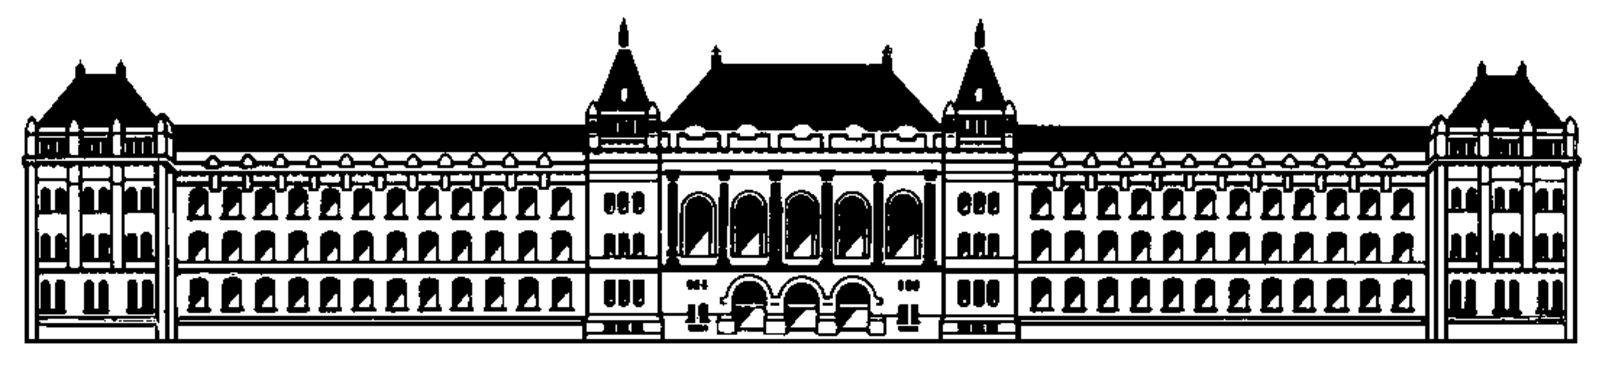
\includegraphics[width=8cm]{bme_skyline}
	%}
	%\end{figure}
	\begin{figure}[h]
		\centering
		%% minipage : subfigure would increase the figure number!!! 
		\begin{minipage}[h]{0.15\textwidth}
			\centering
			%		\includegraphics[height=2.2cm]{gpk_logo_small_OWN.jpg}
			
\includegraphics[height=1.8cm]{GPK_sz.jpg}
		\end{minipage}
		\quad %add desired spacing between images, e. g. ~, \quad, \qquad, \hfill etc. 
		%(or a blank line to force the subfigure onto a new line)
		\begin{minipage}[h]{0.6\textwidth}
			\centering
			%		
\includegraphics[height=2cm]{muegyetem_logo_nagy}
			
\includegraphics[height=1.8cm]{muegyetem_logo_nagy_felirat_nelkul}
		\end{minipage}
		\quad %add desired spacing between images, e. g. ~, \quad, \qquad, \hfill etc. 
		%(or a blank line to force the subfigure onto a new line)
		\begin{minipage}[h]{0.15\textwidth}
			\centering
			
\includegraphics[height=1.8cm]{gttllogo.png}
		\end{minipage}
	\end{figure}
	\hrule
	\vspace{1em}
	% %----------------------------------------------------------------------------------------
	% % % % %	HEADING SECTIONS
	% %----------------------------------------------------------------------------------------
	%\textsc
	{\large Budapesti Műszaki és Gazdaságtudományi Egyetem}\\[0.2em]% % Name of your university/college
	%\textsc
	{\large Gépészmérnöki Kar}\\[0.2em] % % Major heading such as course name
	%\textsc
	{\large Gépgyártástudomány és -technológia Tanszék}\\[0.2em] % % Minor heading such as course title
	{\large Szakdolgozat}  % % tantárgy
	% %----------------------------------------------------------------------------------------
	% %	TITLE SECTION
	% %----------------------------------------------------------------------------------------
	
	%\HRule \\[0.4cm]
	\vspace{15em}
	
	{\Huge  \scshape 
		\textls{  Digitális admittancia szabályozó stabilitásának vizsgálata}
	}\\[0.4em] % % Title of your document
	%\HRule \\[1.5cm]
	%\vspace{4.5cm}
	
	% %----------------------------------------------------------------------------------------
	% %	AUTHOR SECTION
	% %----------------------------------------------------------------------------------------
	
	\vspace{3em}
	
	{\LARGE \bfseries
		Soós Tamás
	}
	
	\vfill % % Fill the rest of the page with whitespace
	
	
	\begin{minipage}[t]{0.45\textwidth}
	\begin{flushleft}\large
   	\emph{Konzulens:}  \\
    Vizi Máté Benjámin
	\end{flushleft}
	\end{minipage}
	\begin{minipage}[t]{0.45\textwidth}
	\begin{flushright}\large
	\emph{Témavezető:}  \\
	Tóth András
	\\ % % Supervisor's Name
	\end{flushright}
	\end{minipage}\\[3em]
	
	

	{\large
		%\today
		Budapest, 2023.12.13.}\\[2em] % % Date, change the \today to a set date if you want to be precise
	
	
	% %----------------------------------------------------------------------------------------
	
	
\end{titlepage}
\cleardoublepage{}
\phantomsection\pdfbookmark[0]{Szakdolgozat feladatkiírás}{feladatlap}

\cleardoublepage{}
\phantomsection{}
\pdfbookmark[0]{Nyilatkozatok}{Nyilatkozatok}
\thispagestyle{empty}

\includepdf[pages=1,pagecommand={},width=19cm]{./chapters/7-melleklet(SZD&DT&ZV&SZGY_Szabalyzat)_SZD_DT_nyilatkozat.pdf}

\cleardoublepage{}
\pdfbookmark[0]{Köszönetnyilvánítás}{acknowledgements}
\chapter*{Köszönetnyilvánítás}

Szeretném megköszönni a konzulensemnek, Vizi Máténak a számtalan konzultációt. 
Köszönöm Tóth András tanár úrnak a szakmai észrevételeit és a bizalmát.  
Végül nagyon köszönöm a páromnak a rengeteg támogatást a félév során.



\cleardoublepage{}
\phantomsection{}
\pdfbookmark[0]{Kivonat}{kivonat}
\chapter*{Kivonat}

A REHAROB egy egészségügyi robot, mely többek között a sztrók okozta mozgásszervi 
zavar rehabilitációjában alkalmazható. 
%
\replace{
	Az eddigi tesztek során a robot többször került közel instabil állapotba. A stabilitásvesztés könnyen a pácienst is veszélyeztető szituációt idézhet elő.%
}{
	Minden digitálisan szabályozott rendszerhez hasonlóan a REHAROB rendszerben is felmerülhetnek a digitális mintavételezésből adódó jelenségek mint például a digitális mintavételezési időkésésből eredő rezgések melyek a szabályozó stabilitásvesztéséhez vezethet. 
	%
	Egy esetleges stabilitásvesztés pedig könnyen a pácienst is veszélyeztető szituációt idézhet elő.%
}
%


Ebben a dolgozatban a robot kézmoduljának egy egyszerűsített egy dimenziós modelljére készült egy admittancia szabályozó. 
%
A szabályozó pozíció és nyomaték bemenettel 
dolgozik, és egy virtuális másodrendű tömeg-rugó-csillapítás mozgását képes emulálni. 
%
A dolgozat az időkésés stabilitásra gyakorolt hatását tárgyalja mind
folytonos, mind pedig diszkrét időben. 

\cleardoublepage{}
\phantomsection{}
\pdfbookmark[0]{TARTALOMJEGYZÉK}{toc}
\tableofcontents

\cleardoublepage{}
\phantomsection{}
\pdfbookmark[0]{ÁBRÁK JEGYZÉK}{lof}
\listoffigures

\cleardoublepage{}
\phantomsection{}
\pdfbookmark[0]{TÁBLÁZATOK JEGYZÉKE}{lot}
\listoftables

\mainmatter{}

\chapter{Bevezetés}

\begin{figure}[b!]
	\begin{center}
		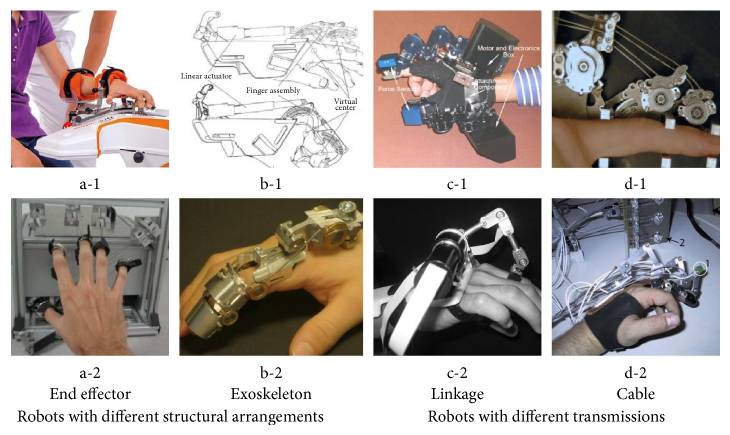
\includegraphics[width=12cm]{images/hand_rehab_robot_types.jpeg}
		\caption{A kéz rehabilitációjánál alkalmazott robotok típusai}\label{fig:hand_rehab_robot_types}
	\end{center}
\end{figure}

A sztrók évente közel 30 000~\citep{Bereczki2023} embert érint ma Magyarországon. A betegség szövődményei között gyakori 
a beszéd-, látás-, vagy mozgászavar, de akár teljes bénulást is okozhat. Az egészségügyi robotok alkalmazása a 
rehabilitáció során elősegítheti a hatékonyabb gyógyulást~\citep{Chang2013}. A kéz rehabilitációjának optimalizálása 
különösen fontos, hiszen alapvető szerepe van a mindennapi feladatok elvégzésében. A kézfej méretéből és ízületeinek számából 
adódóan sajátos kihívásokkal kell megbirkózni egy rehabilitációs robot megtervezésénél.
Az irodalomban megjelenő megoldások főbb típusai közül szemléltet párat az~\ref{fig:hand_rehab_robot_types}. ábra~\citep{Yue2017}.
Két fő kategóriát lehet megkülönböztetni a robot és a felhasználó fizikai kapcsolatát tekintve. Vannak teljesen 
különálló egységek és olyan megoldások, melyeket a felhasználó visel. Az ujjakat lehet külön-külön vagy 
csoportokban mozgatni. A meghajtás lehet elektromos, pneumatikus vagy hidraulikus, de akár piezoelektromos vagy 
alak emlékező fémötvözeten alapuló is. A elektromos meghajtás igen elterjedt, mert széles választék áll rendelkezésre különféle motorokból, 
valamint kedvező az ára és igen megbízható. Az erőátvitel lehet közvetlen, gyakran azonban közvetítő elem (csuklók, kábelek) 
segítségével történik. A páciens aktív részvétele jobb eredményeket mutat a passzív, erőkifejtés nélküli mozgatással 
szemben~\citep{Remsik2016}, ezért elengedhetetlen a páciens mozgási szándékáról valamilyen visszajelzés közvetítése a robot felé.
Ezután a robot a pácienssel összhangban hajthatja végre a gyakorlatot.
A szenzorokat tekintve vannak megoldások melyek a mozgásállapotot mérik (erő, nyomaték, elmozdulás)~\citep{Bauer2021}, de megjelennek 
bioelektromos jeleket mérő szenzorok is~\citep{Satakogiou}. 

A hardveren túl a szabályozó típusa szerint is csoportosíthatók a különböző megoldások. Vannak erőszabályozáson 
alapuló rendszerek~\citep{kovacs2003dynamics}, de leggyakoribbak a hibrid erő és 
pozíció szabályozáson alapuló egységek~\citep{Hua2019,Xie2021}, azonban vannak például fuzzy szabályozáson alapuló architektúrák is~\citep{Hu2023}.
A hibrid erő és pozíció szabályozásnak számos előnye van a tisztán pozíció vagy erő visszacsatolással 
szemben~\citep{hogan1984Impedance,hogan1985ImpedancePART1,hogan1985ImpedancePART2,hogan1985ImpedancePART3,kovacs2003dynamics,stepan2001vibrations}.
Ez a szabályozó típus kifejezetten jól alkalmazható ember-robot interakciót igénylő feladatoknál, mint amilyen 
a rehabilitáció is. A szabályozó referencia jele nem csupán 
az elérni kívánt pozíció vagy kifejtett nyomaték, hanem a mozgásállapot és a kifejtett
nyomaték közötti összefüggés. Ezt az összefüggést egy 
tömeg-rugó-csillapitás modell adja meg a továbbiakban, mely a következő alakban
írható fel: 
\begin{align}
    M_\RM e \ddot \theta + B_\RM e \dot \theta + K_\RM e (\theta - \theta_\RM r) = \tau_\RM e\,.
\end{align}
A modell három paraméterrel rendelkezik, $M_\RM e$ a rendszer előírt tehetetlensége, 
$B_\RM e$ a viszkózus csillapítása, és $K_\RM e$ a rugóállandója. 
$\theta_\RM r$ és $\tau_\RM e$ az elérni kívánt pozíció és a rendszerre ható külső nyomaték. 

\begin{figure}[t!]
	\begin{center}
		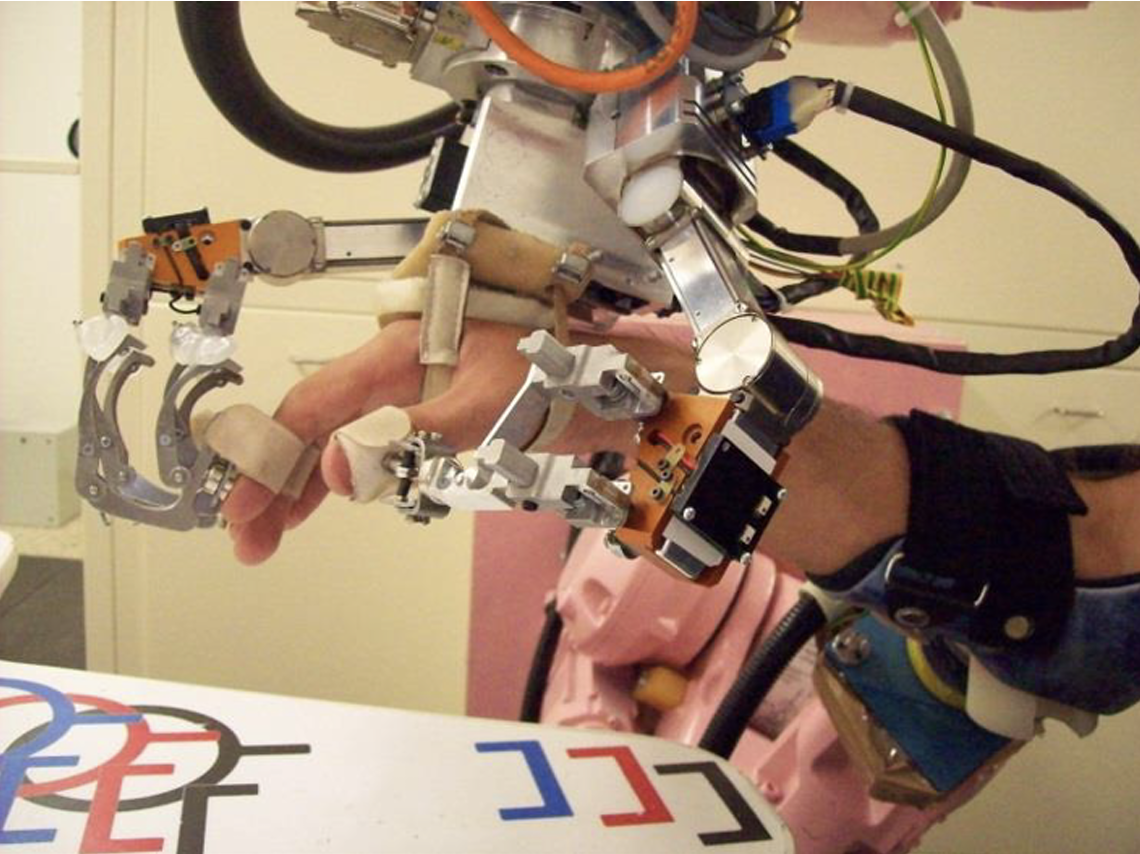
\includegraphics[width=8cm]{images/reharob_hand_module.png}
		\caption{A REHAROB rehabilitációs robot kézmodulja}\label{fig:reharob_hand_module}
	\end{center}
\end{figure}

Ez a dolgozat elsősorban az Országos Mozgásszervi Intézetben megépített REHAROB 3.0 
rehabilitációs robot kézmoduljában alkalmazott robotujj hatékonyságának javításához kíván hozzájárulni.
A robot kézmodulja az~\ref{fig:reharob_hand_module}. ábrán látható.
A REHAROB 3.0 rehabilitációs robot működhet passzív vagy aktív üzemmódban. Passzív üzemmódban előre felvett 
mozgáspályákon halad végig, míg aktív üzemmódban előre beprogramozott hétköznapi feladatok 
kivitelezésében asszisztálja a pácienst. A kézmodul közvetlen hajtással rendelkezik. A mutatóujj, a középső ujj és a
gyűrűs ujj együtt, míg a hüvelyujj külön mozgatható. A kisujj nem vesz részt a mozgatásban. Cserélhető ortézisek 
teszik lehetővé, hogy különböző kéz mérettel rendelkező páciensek is használhassák a berendezést.



A dolgozat a robotujj egyszerűsítettt egyszabadságfokú modelljére alkalmazott admittancia szabályozó stabilitását vizsgálja.
A digitális rendszerek stabilitására nagy hatással lehet az időkésés~\citep{stepan1989retarded,stepan2001vibrations}, így a 
stabilitásvizsgálat során fő szempont lesz ennek a hatásnak az elemzése.


% \begin{itemize}
%     \item Irtech: 
%     \citep{lantos2016iranyitasi1,lantos2016iranyitasi2,lantos2017iranyitasi3}
%     + MOGIS VALAMI + NEMZETKÖZI
    
%     \item Kálmán: state space, megfigyelő, stb: \citep{kalman1960new,kalman1963controllability,kalman1963mathematical,kalman1960contributions}
    
% \end{itemize}

\chapter{Fizikai modell}\label{chap:physical_system}

Ebben a fejezetben a robotujj \alert{egyetlen} \add{EZT HOGY ÉRTED? 1DOF MODELLT CSINÁLUNK AZ RENDBEN, DE A ROBOTUJJBAN 5 MOTOR VAN} motorjának fizikai modellje kerül bevezetésre. A kapott dinamikai leírás
lehetővé teszi az időkéséssel kiegészített stabilitásvizsgálatot. 

\section{Egyenáramú motor dinamikája}

\begin{figure}[b!]
\begin{center}
%\phantomsection{}
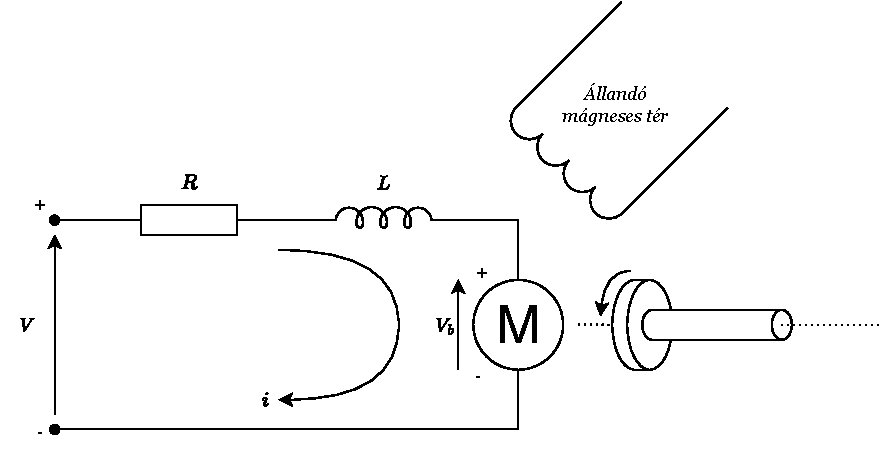
\includegraphics[width=\textwidth]{images/motor_model_electric.pdf}
\caption{Az egyenáramú motor áramköri diagramja}
\label{fig:dc_motor_electric}
\end{center}
\end{figure}

A robot motorjának modelljét a~\ref{fig:dc_motor_electric}. ábra szemlélteti. 
A felhasznált motor feltételezetten állandó gerjesztésű. Kifejtett nyomatéka a 
Biot--Savart-törvény szerint arányos a forgórészen átfolyó árammal. A forgórészben
indukált feszültség pedig arányos annak szögsebességével. 

A Lenz-törvény alapján 
\begin{equation}\label{eq:lenz_torque}
\begin{split}
    \tau_\RM m &= K_\RM \tau i, \\
    V_\RM b &= K_\RM e \dot\theta,
\end{split}
\end{equation}
ahol $K_\RM \tau$ a nyomatékállandó, $K_\RM e$ a sebesség-feszültség állandó, $\tau_\RM m$ a kifejtett 
nyomaték, $i$ a rotor árama, $V_\RM b$ a rotorban indukált feszültség és $\dot\theta$ a rotor szögsebessége.

Az energiamegmaradás törvénye alapján a két konstans értéke SI mértékegységben kifejezve megegyezik:
\begin{align}
    K_\RM m \stackrel{\text{def}}{=} K_\RM \tau = K_\RM e,
\end{align}
így a következőkben $K_\RM m$ paraméterként jelennek meg. 

A forgórész áramkörére Kirchhoff I. törvénye alapján felírható
\begin{align}\label{eq:armature_circuit}
    V - Ri - L\DIFF{i}{t} - K_\RM m\dot\theta = 0,
\end{align}
ahol $R$ a forgórész tekercsének ellenállása, $L$ a tekercs induktivitása, 
$K_\RM m$ a motorállandó, $V$ a motor feszültsége, $i$ a motoráram és $\theta$ a szögelfordulás.


A forgórészt merev testnek tekintve, annak mozgásegyenlete a dinamika alaptétele és a~\ref{fig:dc_motor_mechanical}. számú 
szabadtest-ábra alapján a következő alakban írható fel:
\begin{align}\label{eq:rotor_dynamics}
    J\ddot\theta + B_\RM m\dot\theta = \tau_\RM m + \tau_\RM e,
\end{align}
ahol $J$ a forgórész tehetetlensége, $B_\RM m$ a viszkózus csillapítási együttható, 
$K_\RM m$ a motorállandó, $\theta$ a szögelfordulás, $i$ a motoráram, $\tau_\RM m$ a motor által kifejtett nyomaték 
és $\tau_\RM e$ a forgórészre ható külső nyomaték. 
%
A~\eqref{eq:armature_circuit} és~\eqref{eq:rotor_dynamics} egyenletek egyértelműen leírják a 
rendszer időtartománybeli viselkedését.

\begin{figure}[t!]
	\begin{center}
		%\phantomsection{}
		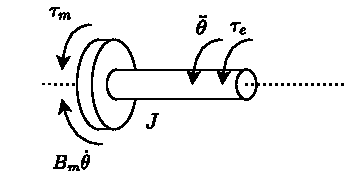
\includegraphics[width=9cm]{images/motor_model_mechanical.pdf}
		\caption{Az egyenáramú motor szabadtest ábrája}
		\label{fig:dc_motor_mechanical}
	\end{center}
\end{figure}

A további vizsgálathoz kedvezőbb a differenciálegyenleteket állapottér modellként felírni.
Az állapottér modell általánosan~\citep{kalman1963mathematical}
\begin{equation}\label{eq:state_space_generic}
\begin{split}
    \dot{\BF x} &= \BF A \BF x + \BF B \BF u\,,\\
    \BF y &= \BF C \BF x + \BF D \BF u
\end{split}
\end{equation} 
alakban írható fel. Legyen 
\begin{equation}
	\BF x := [\theta~~\dot \theta~~i]^{\mathsf T}
\end{equation}
az állapotvektor, emellett
\begin{equation}\label{eq:uinput27}
	\BF u := [\tau_\RM e~~V]^{\mathsf T}
\end{equation} 
a bemeneti vektor és \(y := \theta\) a kimenet.

A~\eqref{eq:armature_circuit} és a~\eqref{eq:rotor_dynamics} egyenleteket átrendezve 
az  \(\BF A\) \alert{állapot-átmeneti mátrix}\add{EZT NEM RENDSZERMÁTRIXNAK HÍVJUK?}, a \(\BF B\) bemeneti mátrix, a \(\BF C\) kimeneti mátrix és a \(\BF D\) segédmátrix az 
\begin{equation}\label{eq:state_space}
    \begin{split}
        \BF A &= 
        \begin{bmatrix}
            0 & 1 & 0 \\
            0 & -\frac{B_\RM m}{J} & \frac{K_\RM m}{J} \\
            0 & -\frac{K_\RM m}{L} & -\frac{R}{L} \\
        \end{bmatrix}\,,\\
        \BF B &=
        \begin{bmatrix}
            0 & 0 \\
            1 & 0 \\
            0 & 1 \\
        \end{bmatrix}\,,\\
        \BF C &=
        \begin{bmatrix}
            1 & 0 & 0 \\
        \end{bmatrix}\,,\\
        \BF D &= \BF 0
    \end{split}
\end{equation}
alakban származtatható. 

A későbbiekben ismertetett kísérleti összeállítás paraméterei 
nem teszik lehetővé a forgórész áramának modellezését, ehhez bővebb indoklás az \ref{chap:experiment}.\,fejezetben található. 
%
Az induktivitással kiegészített modell mellett mindig megjelenik az 
induktivitás nélküli modell, ahol szükséges. 
%
Az egyszerűsített állapottér modell állapotvektora 
\(\BF x = [\theta~~\dot \theta]^{\mathsf T}\), az \(\BF u\) bemeneti vektora változatlan (lásd \eqref{eq:uinput27}), 
\(\BF A\), \(\BF B\), \(\BF C\) és \(\BF D\) mátrixa pedig 
%
\begin{equation}\label{eq:state_space_reduced}
    \begin{split}
        \BF A &= 
        \begin{bmatrix}
            0 & 1 \\
            0 & -\frac{B_\RM m R + K^2_\RM m}{JR} \\
        \end{bmatrix}\,,\\
        \BF B &=
        \begin{bmatrix}
            0 & 0 \\
            \frac{1}{J} & \frac{K_\RM m}{JR} \\
        \end{bmatrix}\,,\\
        \BF C &=
        \begin{bmatrix}
            1 & 0 \\
        \end{bmatrix}\,,\\
        \BF D &= \BF 0\,.
    \end{split}
\end{equation}

Az állapottér modellt felhasználva a frekvenciatartománybeli vizsgálatokhoz felírhatóak a rendszer 
szög-nyomaték és szög-feszültség átviteli függvényei, ezek általános alakja az alábbi:
\begin{align}\label{eq:transfer_generic}
    \frac{Y(s)}{U(s)} = \BF C{\left(s \BF I - \BF A\right)}^{-1} \BF B\,,
\end{align}
ahol $\BF I$ az identitás mátrix.

Behelyettesítve~\eqref{eq:state_space} 
paramétereit~\eqref{eq:transfer_generic} alapján a karakterisztikus polinom a
\begin{align}\label{eq:characteristic_polynomial}
    p(s) = s\left(JLs^2 + \left(B_\RM m L + JR\right)s + K_\RM m^2 + B_\RM m R\right)
\end{align}
alakban adódik. Az átviteli függvények pedig ez alapján
\begin{equation}\label{eq:transfer_function}
    \begin{split}
        \frac{\theta(s)}{\tau_\RM e(s)} &= \frac{Ls + R}{p(s)}\,,\\
        \frac{\theta(s)}{V(s)} &= \frac{K_\RM m}{p(s)}\,.
    \end{split}
\end{equation}

Az induktivitás elhanyagolása esetén az előzőekhez hasonlóan származtatható a a karakterisztikus polinom:
\begin{align}\label{eq:characteristic_polynomial}
    p(s) = s\left(JRs + K_\RM m^2 + B_\RM m R\right),
\end{align}
valamint az átviteli függvények szintén egyszerűsödnek:
\begin{equation}\label{eq:transfer_function}
    \begin{split}
        \frac{\theta(s)}{\tau_\RM e(s)} &= \frac{R}{p(s)}\,,\\
        \frac{\theta(s)}{V(s)} &= \frac{K_\RM m}{p(s)}.
    \end{split}
\end{equation}

\section{Egyenáramú motor stabilitása}
A motormodell stabilitási tulajdonságai a~\eqref{eq:characteristic_polynomial} egyenletben szereplő karakterisztikus 
polinom segítségével meghatározhatók.
A karakterisztikus polinom egyik zérusa az origóban helyezkedik el. Ebből következik, hogy a rendszer
egységugrás bemenetre korlátlanul nagy szögelfordulással válaszol. Ez utóbbi a jelen alkalmazásban nem elfogadható. 
Ha a szabályozókör visszacsatoló ága megszakad, a motor a megengedhető mozgástartományon kívülre fordulhat.
A biztonságos működéshez szükséges például egy végálláskacsolót beépíteni, mely segítségével a motor 
mozgása a szabályozástól függetlenül is az előírt tartományon belülre korlátozható.

\section{Megfigyelhetőség}\label{chap:observability}
A felhasznált szenzorok számának minimalizálása érdekében a lehető legkevesebb belső állapot közvetlen mérése 
a cél. A továbbiakban egyedül a szögelfordulás áll elő közvetlen mérésből. 
A szabályozó teljes állapotvisszacsatolásra épül, így a kimenet mérésével minden további belső állapot 
megfigyelhető kell legyen. 
A~\eqref{eq:state_space_generic} és~\eqref{eq:state_space} egyenletek alapján a kimeneti megfigyelhetőség feltétele, hogy a
\begin{align}\label{eq:observability_generic}
    \left[\begin{array}{c}
        \BF{C} \\ \hline
        \BF{CA} \\ \hline
        \BF C \BF A^2
    \end{array}\right]
\end{align}
mátrix legyen maximális rangú. A feltételben szereplő mátrixot a motorparaméterekkel kifejezve 
a~\eqref{eq:state_space} egyenlet alapján:
\begin{align}
    \begin{bmatrix}
        1 & 0 & 0 \\
        0 & 1 & 0 \\
        0 & -\frac{B_\RM m}{J} & \frac{K_\RM m}{J}
    \end{bmatrix},
\end{align}
mely redukált lépcsős alakra hozható:
\begin{align}
    \begin{bmatrix}
        1 & 0 & 0 \\
        0 & 1 & 0 \\
        0 & 0 & 1
    \end{bmatrix}.
\end{align}
Ez valóban maximális rangú, tehát a rendszer minden állapota megfigyelhető a szögelfordulás méréséből.

Az induktivitást elhanyagolva a megfigyelhetőség feltétele
még egyszerűbb alakkal rendelkezik, a megfigyelhetőségi mátrix ekkor:
\begin{align}
	\left[\begin{array}{c}
		\BF{C} \\ \hline
		\BF{CA} \\
	\end{array}\right].
\end{align}
Behelyettesítve az egyszerűsített modell \eqref{eq:state_space_reduced} paramétereit ez a megfigyelhetőségi mátrix azonnal redukált lépcsős alakban adódik:
\begin{align}
    \begin{bmatrix}
        1 & 0 \\
        0 & 1 \\
    \end{bmatrix}.
\end{align}
Ezáltal a rendszer minden állapota megfigyelhető ebben az esetben is. 


\clearpage


\section{Irányíthatóság}\label{chap:controllability}
A szabályozó akkor tudja követni a számára előírt impedanciamodellt, 
ha megfelelő bemeneti feszültség alkalmazásával eljuttatható az előírt állapotba~\citep{kalman1963controllability}.

A rendszer pólusai áthelyezhetők kell legyenek az impedanciamodell pólusaiba, 
ehhez pedig a rendszer teljesen állapot irányítható kell legyen.
A~\eqref{eq:state_space_generic} egyenlet állapottér modellje alapján a teljes állapot irányíthatóság feltétele, hogy a
\begin{align}\label{eq:controllability_generic}
    \left[\begin{array}{c|c|c}
        \BF{B} & \BF{AB} & \BF A^2 \BF B
    \end{array}\right]
\end{align}
irányíthatósági mátrix maximális rangú legyen. 
Felhasználva a~\eqref{eq:state_space} kifejezés paramétereit a~\alert{\eqref{eq:observability_generic}} \add{EZ ITT TUTI NEM JÓ EGYENLET HIVATKOZÁS} feltételben szereplő mátrix
\begin{align}
    \begin{bmatrix}
        0 & 0 & \frac{K_\RM m}{JL} \\
        0 & \frac{K_\RM m}{JL} & -\frac{K_\RM m\left(B_\RM m L + JR\right)}{J^2 L^2} \\
        \frac{1}{L} & -\frac{R}{L^2} & -\frac{K^2_\RM m L + JR^2}{J L^3} \\
    \end{bmatrix},
\end{align}
alakba írható át \add{HOGYAN JÖHET KI EZ 3x3-ASRA, ENNEK NEM 3x6-NAK KÉNE LENNIE?}. Továbbá ez a mátrix redukált lépcsős alakban
\begin{align}
    \begin{bmatrix}
        1 & 0 & 0 \\
        0 & 1 & 0 \\
        0 & 0 & 1 \\
    \end{bmatrix},
\end{align}
mely mátrix rangja megegyezik sorainak számával, így az teljes állapot irányíthatóság feltétele teljesül.

Az induktivitást elhanyagolva az irányíthatósági feltételben megjelenő mátrix 
\begin{align}
    \left[\begin{array}{c|c}
        \BF{B} & \BF{AB}
    \end{array}\right].
\end{align}
Az egyszerűsített modell paramétereit behelyettesítve 
a
\begin{align}
    \begin{bmatrix}
        1 & 0 \\
        0 & 1 \\
    \end{bmatrix}
\end{align}
irányíthatósági mátrixot kapjuk.
Ez láthatóan megfelel a feltételnek, tehát az induktivitást elhanyagoló modell is teljes állapot irányítható.



\chapter{Szabályozó modellezése}\label{chap:controller}

Az ebben fejezetben levezetett állapotmegfigyelő és a szögelfordulás közvetlen mérése
együtt a rendszer teljes állapotvektorát elérhetővé teszi a szabályozó számára. A rendszer pólusai a~\ref{chap:controllability}.\ fejezetben
vizsgált irányíthatósági feltétel teljesülése miatt szabadon áthelyezhetők. 
Az impedanciamodell által előírt dinamikai összefüggés részben teljes állapot-visszacsatolással érhető el, 
azonban a nyomatékválasz külön figyelmet igényel.  

\section{Állapotmegfigyelő}\label{chap:observer}
Ahogy a jelen alkalmazásban is, sokszor nem áll rendelkezésre az állapot-visszacsatoláshoz szükséges 
összes belső állapotot közvetlen mérésből. Ilyenkor egy állapotmegfigyelő adhat becslést az ismeretlen 
állapotokra~\citep{kalman1960new,OgataModernControl}. Elkülönítve a mért és a becsült állapotokat~\eqref{eq:state_space_generic} 
felírható:
\begin{equation}\label{eq:observer_state}
    \begin{split}
    \left[\begin{array}{c}
        \dot x_\RM a \\ \hline
        \dot{\BF x}_\RM b
    \end{array}\right]
    &=
    \left[\begin{array}{c|c}
        A_\RM{aa} & \BF A_\RM{a b} \\ \hline
        \BF A_\RM{ba} & \BF A_\RM{bb}
    \end{array}\right]
    \left[\begin{array}{c}
        x_\RM a \\ \hline
        \BF x_\RM b
    \end{array}\right]
    +
    \left[\begin{array}{c}
        B_\RM a \\ \hline
        \BF B_\RM b
    \end{array}\right]
    \begin{bmatrix}
        \tau_\RM e \\
        V \\
    \end{bmatrix}\,,\\
    y &= 
    \left[\begin{array}{c|c}
        1 & \BF 0
    \end{array}\right]
    \left[\begin{array}{c}
        x_\RM a \\ \hline
        \BF x_\RM b
    \end{array}\right]
    \end{split}
\end{equation}
alakban, ahol $x_\RM a = \theta$ a mért szögelfordulás és 
$\BF{x}_\RM b = [\dot \theta~~i]^{\mathsf T}$ jelöli a becsült állapotokat.
A továbbiakban jelölje $\tilde{*}$ a becsült állapotok megfigyelő által számított értékeit. Legyen
\begin{align}\label{eq:observer_params}
    \begin{split}
    \hat{\BF A} &= \BF A_\RM{bb} - \BF K_\RM e \BF A_\RM{ab}\,,\\
    \hat{\BF B} &= \hat{\BF A} \BF K_\RM e + \BF A_\RM {ba} - \BF K_\RM e A_\RM {aa}\,,\\
    \hat{\BF F} &= \BF B_\RM b - \BF K_\RM e B_\RM a\,,
    \end{split}
\end{align}
ahol $\hat{\BF A}$ a megfigyelő belső állapotának (továbbiakban $\tilde{\BF \eta}$) 
dinamikáját adja meg, $\hat{\BF B}$ és $\hat{\BF F}$ a mért, illetve a becsült állapotok 
bemeneti mátrixai és $\BF K_\RM e$ a megfigyelő hibájának a visszacsatoló mátrixa. 
A megfigyelő belső állapota és a becsült állapotváltozók közötti összefüggés ekkor
\begin{align}
    \begin{split}
    \BF \eta &= \BF x_\RM b - \BF K_\RM e y\,,\\
    \tilde{\BF \eta} &= \tilde{\BF x}_\RM b - \BF K_\RM e y
    \end{split}
\end{align}
alakban adható meg. A megfigyelő belső állapotának dinamikája
\begin{align}
    \begin{split}
    \dot{\tilde{\BF \eta}} = \hat{\BF A} \tilde{\BF \eta} + \hat{\BF B} y + \hat{\BF F} u\,.
    \end{split}
\end{align}
Végül~\eqref{eq:observer_state} kimeneti egyenletének átalakításával a rendszer becsült állapotvektora
\begin{align}
    \tilde{\BF x} = \hat{\BF C} \tilde{\BF \eta} + \hat{\BF D} y\,,
\end{align}
ahol
\begin{align}
    \hat{\BF C} = 
    \left[\begin{array}{c}
        \BF 0 \\ \hline
        \BF I_{n-1}
    \end{array}\right]\,,
    \quad
    \hat{\BF D} = 
    \left[\begin{array}{c}
        1 \\ \hline
        \BF K_\RM e
    \end{array}\right]\,.
\end{align}
Ez a teljes állapotvektor, így tartalmazza a mért szögelfordulást is.

\section{Pozíció szabályozás}
Az előírt modell két független bemenettel rendelkezik. Jelen esetben a szögelfordulásra és a 
külső nyomatékra előírt válasz viszont csak az amplitúdójukban térnek el. Ezt kihasználva először kizárólag a szögelfordulás referencia jelére előírt válasz alapján 
kerülnek áthelyezésre a pólusok. Teljes állapot-visszacsatolás esetén a motorra kapcsolt feszültség
\begin{align}\label{eq:position_control_voltage}
    V = K_\RM r \theta_\RM r -\BF K \tilde{\BF x}
\end{align}
összefüggéssel adható meg, 
ahol $\BF K$ az állapot-visszacsatolási mátrix, 
$K_\RM r$ a referencia jel erősítési tényezője és
$\theta_\RM r$ az előírt szögelfordulás. A~\eqref{eq:position_control_voltage} egyenlet felhasználásával
a~\eqref{eq:state_space_generic} egyenletben szereplő állapottér modell belső állapotának dinamikája
\begin{align}\label{eq:position_control_law_state}
    \dot{\BF x} = \BF A \BF x + \BF B_\RM V\left[K_\RM r \theta_\RM r - \BF K \tilde{\BF x}\right] + \BF B_\RM \tau \tau_\RM e
\end{align}
alakra írható át. A $\BF B$ mátrix oszlopai elkülönítve $\BF B_\RM V$ és $\BF B_\RM \tau$ paraméterekként jelennek meg.
Legyen a továbbiakban a motor becsült állapotai és a megfigyelő által számított állapotok közötti hiba:
\begin{align}
    \BF e = \BF x_\RM b - \tilde{\BF x}_\RM b\,.
\end{align}
A~\eqref{eq:position_control_law_state} egyenlet a megfigyelő által számított állapotok 
vektorának kiküszöbölésével
\begin{align}
    \dot{\BF x} = \left(\BF A - \BF B_\RM V \BF K\right) \BF x + 
    \BF B_\RM V \BF K_\RM b \BF e + 
    \BF B_\RM \tau \tau + 
    \BF B_\RM V K_\RM r \theta_\RM r
\end{align}
alakra hozható. A valós és becsült állapot közötti hiba dinamikája~\eqref{eq:observer_state} felhasználásával
\begin{equation}
    \begin{split}
    \dot{\BF x}_\RM b &= \BF A_\RM{ba} x_\RM a + \BF A_\RM{bb} \BF x_\RM b + 
    \BF B_\RM{Vb} V + \BF B_\RM{\tau b} \tau_\RM e\,,\\
    \dot{\tilde{\BF x}}_\RM b &= \left(\BF A_\RM{bb} - \BF K_\RM e \BF A_\RM{ab}\right) \tilde{\BF x}_\RM b +
    \BF A_\RM{ba} x_\RM a +
    \BF K_\RM e \BF A_\RM{ab} \BF x_\RM b +
    \BF B_\RM{Vb} V\,.
    \end{split}
\end{equation}
Melyeket kivonva egymásból az \(\BF e\) hiba időbeli változására az alábbi egyenlet adódik:
\begin{align}
    \dot{\BF e} = \left(\BF A_\RM{bb} - \BF K_\RM e \BF A_\RM{ab}\right) \BF e + \BF B_\RM{\tau b} \tau_\RM e\,.
\end{align}
A rendszer dinamikája blokk mátrix alakban a következő:
\begin{align}\label{eq:pos_control_dynamics}
    \begin{bmatrix}
        \dot{\BF x} \\
        \dot{\BF e}
    \end{bmatrix}
    =
    \begin{bmatrix}
        \BF A - \BF B_\RM V \BF K & \BF B_\RM V \BF K_\RM b \\
        \BF 0 & \BF A_\RM{bb} - \BF K_\RM e \BF A_\RM{ab}
    \end{bmatrix}
    \begin{bmatrix}
        \BF x \\
        \BF e
    \end{bmatrix}
    +
    \begin{bmatrix}
        \BF B_\RM \tau & \BF B_\RM V K_\RM r\\
        \BF B_\RM{\tau b} & \BF 0
    \end{bmatrix}
    \begin{bmatrix}
        \tau_\RM e \\
        \theta_\RM r
    \end{bmatrix}.
\end{align}

A referencia jel erősítési tényezője a teljes rendszer átviteli függvénye alapján a végérték tétellel határozható meg.
A rendszer válaszának végértéke~\eqref{eq:pos_control_dynamics} szerint egységugrás bemenetre:
\begin{equation}\label{eq:input_gain}
    \lim_{s \to 0}~s \cdot \theta(s) = 
    \lim_{s \to 0}~-\frac{K_\RM m K_\RM r M_\RM e}{JL(p-s)(M_\RM e s^2 + B_\RM e s + K_\RM e)}\frac{s}{s} =
    -\frac{K_\RM m K_\RM r M_\RM e}{JLpK_\RM e}\,,
\end{equation}
ahol \(p\) a megfigyelő pólusa.
Feltételezve, hogy az összesen kettő darab szabadon választható pólus értéke ugyanaz, 
és ez az érték valós. Az erősítési tényező ez alapján:
\begin{equation}\label{eq:input_coeff}
    K_\RM r = -\frac{JLpK_\RM e}{K_\RM m M_\RM e}\,.
\end{equation}

A megfigyelő \(\BF e\) belső hibájának megváltozása nem csak a pillanatnyi belső hibától függ. Még ha a 
\(\BF A_\RM{bb} - \BF K_\RM e \BF A_\RM{ab}\) mátrix sajátértékei
mind negatív valós résszel is rendelkeznek, a megfigyelő belső hibája akkor sem tart feltétlenül nullához külső nyomaték jelenlétében.
Amennyiben a \(\BF A - \BF B_\RM V \BF K\) mátrix sajátértékei is mind negatív valós résszel rendelkeznek,
a teljes rendszer exponenciálisan stabil, de a külső nyomatékra adott válasz végértéke eltér az impedanciamodell
által előírt értéktől. Ez a szabályozó még nem felel meg az alkalmazás előírásainak. A rendszer válasza a pozíció referencia bemenetre adott egységugrás jelre a~\ref{fig:observer_controller_pos_resp}. ábrán látható. 
Az alkalmazott paramétereket az~\ref{tab:observer_controller_pos_resp}. táblázat tartalmazza. 
\begin{table}[H]
    \small\centering
    \caption{Pozíció referencia bemenetre adott egységugrás jelnél alkalmazott paraméterek}\label{tab:observer_controller_pos_resp}
    \tabcolsep=1pt
    \begin{tabular}{l>{~}l>{\quad}rl}
        \toprule
        \multicolumn{2}{c}{Szimbólum és paraméter név} & \multicolumn{2}{c}{Érték} \\ \midrule
        \(M_\RM e\) & Előírt tehetetlenség & 1 & \(\RM{kg\cdot m^2}\) \\
        \(B_\RM e\) & Előírt viszkózus csillapítás & 4 & \(\RM{kg\cdot m^2\cdot s^{-1}}\) \\
        \(K_\RM e\) & Előírt rugóállandó & 16 & \(\RM{kg\cdot m^2\cdot s^{-2}}\) \\
        \(J\) & Motor tehetetlensége & 0.01 & \(\RM{kg\cdot m^2}\) \\
        \(K_\RM m\) & Motor nyomatékállandója & 0.01 & \(\RM{Nm\cdot A^{-1}}\) \\
        \(B_\RM m\) & Motormodell viszkózus csillapítása & 0.1 & \(\RM{kg\cdot m^2\cdot s^{-1}}\) \\
        \(L\) & Motor induktivitása & 0.2 & H \\
        \(R\) & Motor ellenállása & 1 & \(\Omega\) \\
        \bottomrule
    \end{tabular}
\end{table}
Az áthelyezett pólusok \(P = [-2.00 - 3.46i~~-2.00 + 3.46i~~-8.00]\) 
és a megfigyelő pólusai \(P_\RM o = [-8.00~~-8.00]\). Az első két áthelyezett pólust az impedanciamodell
határozza meg.
\begin{figure}[H]
    \begin{center}
    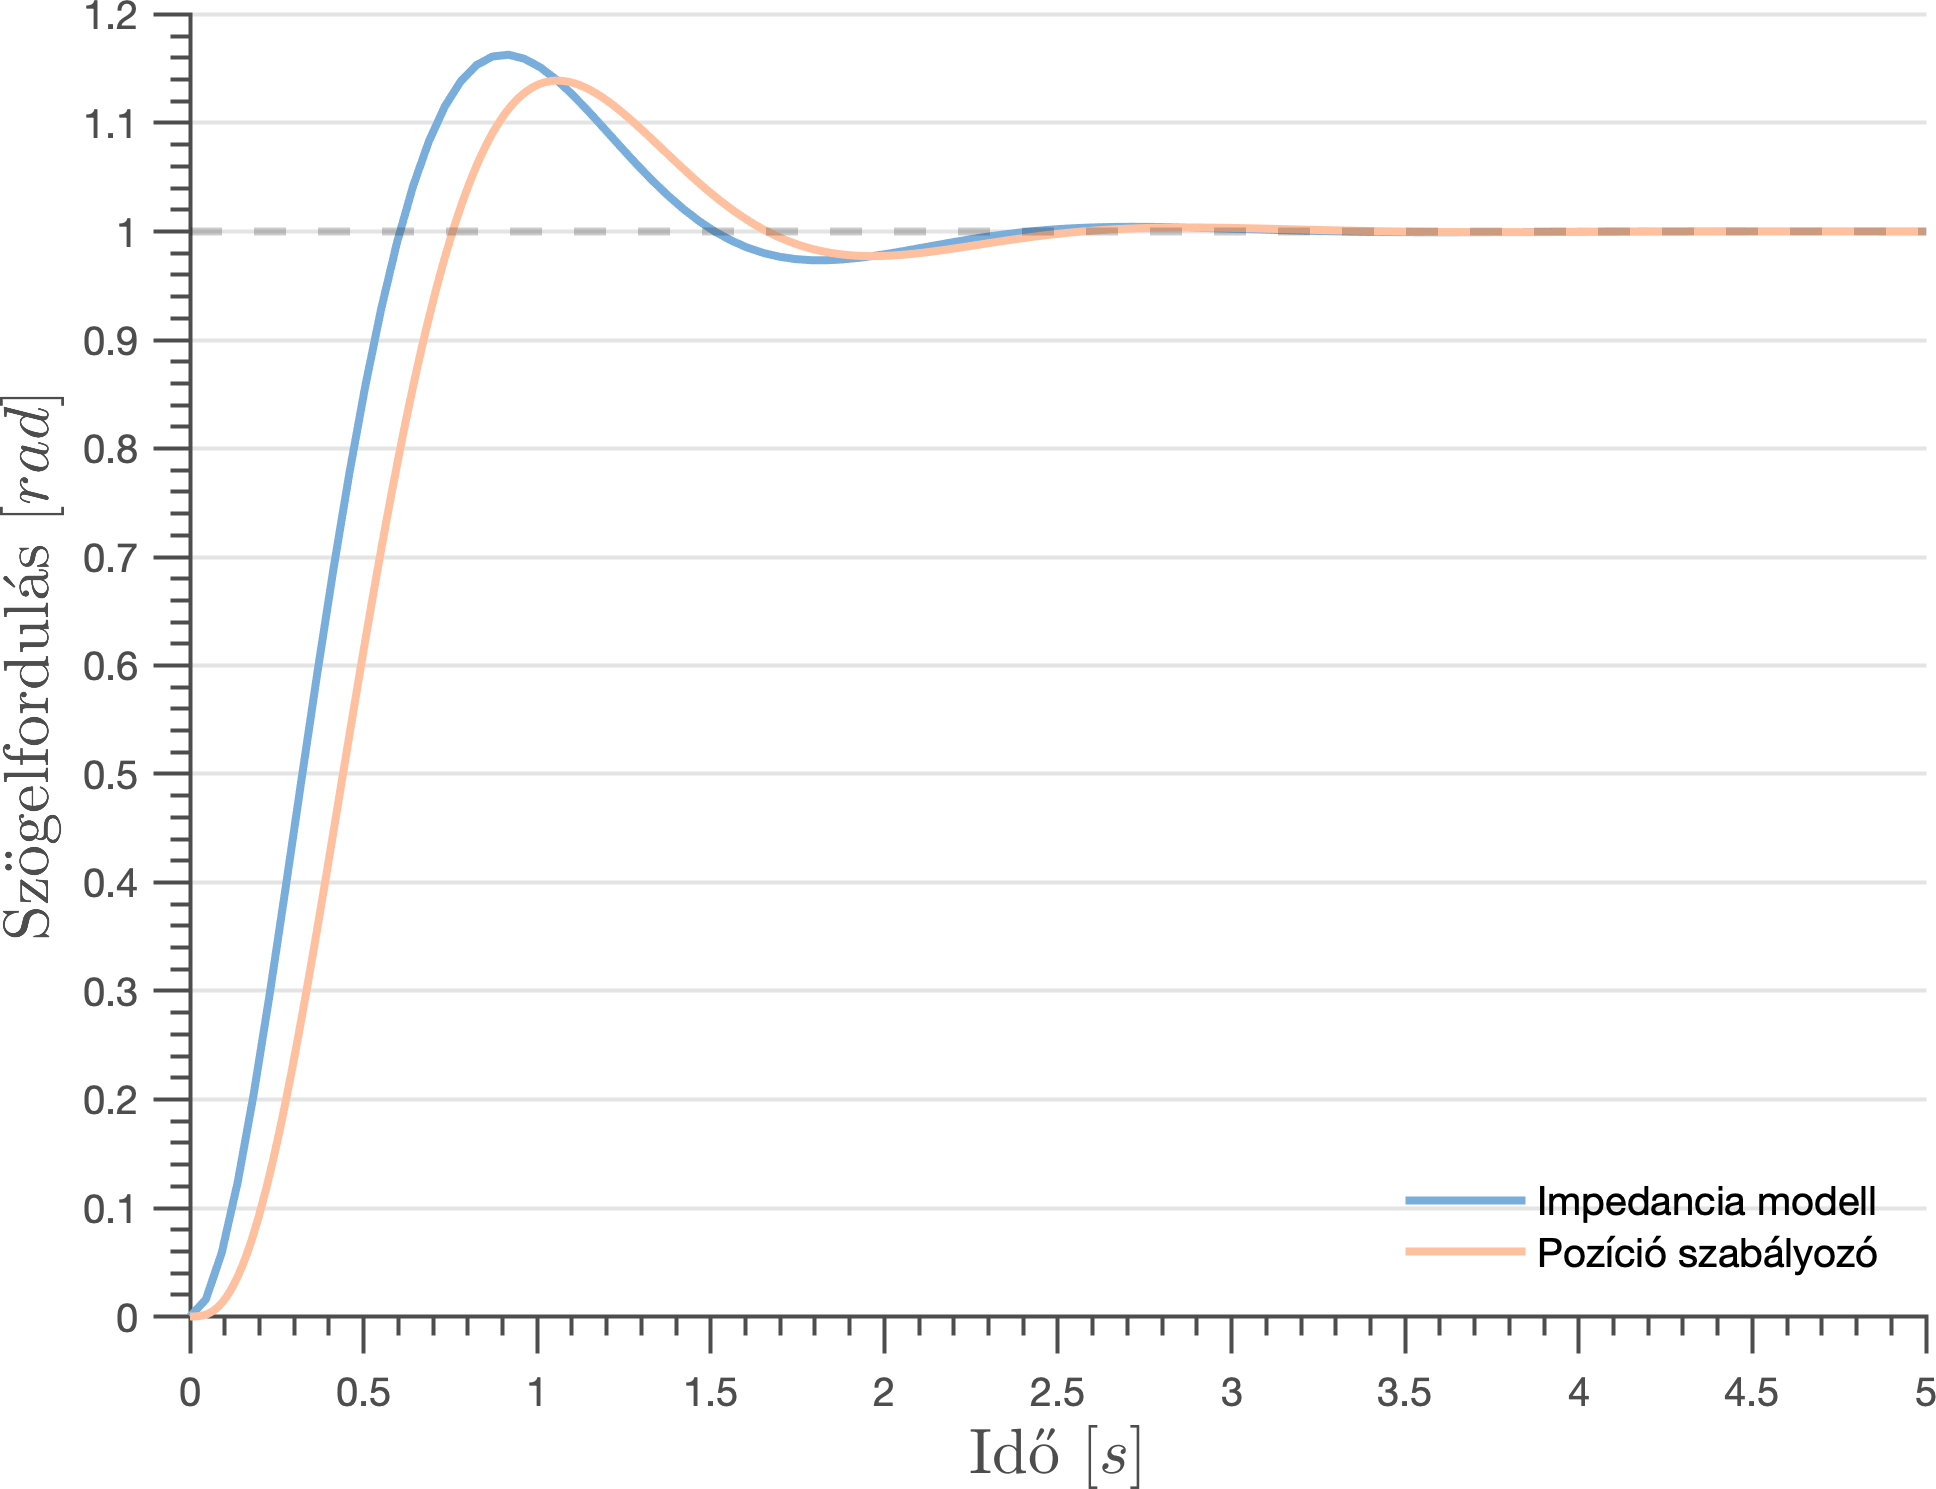
\includegraphics[width=14cm]{images/observer_controller_pos_resp.png}
    \caption{Az impedanciamodell és a szabályozó összehasonlítása pozíció egységugrás bemenetre}\label{fig:observer_controller_pos_resp}
    \end{center}
\end{figure}
\begin{figure}[H]
    \begin{center}
    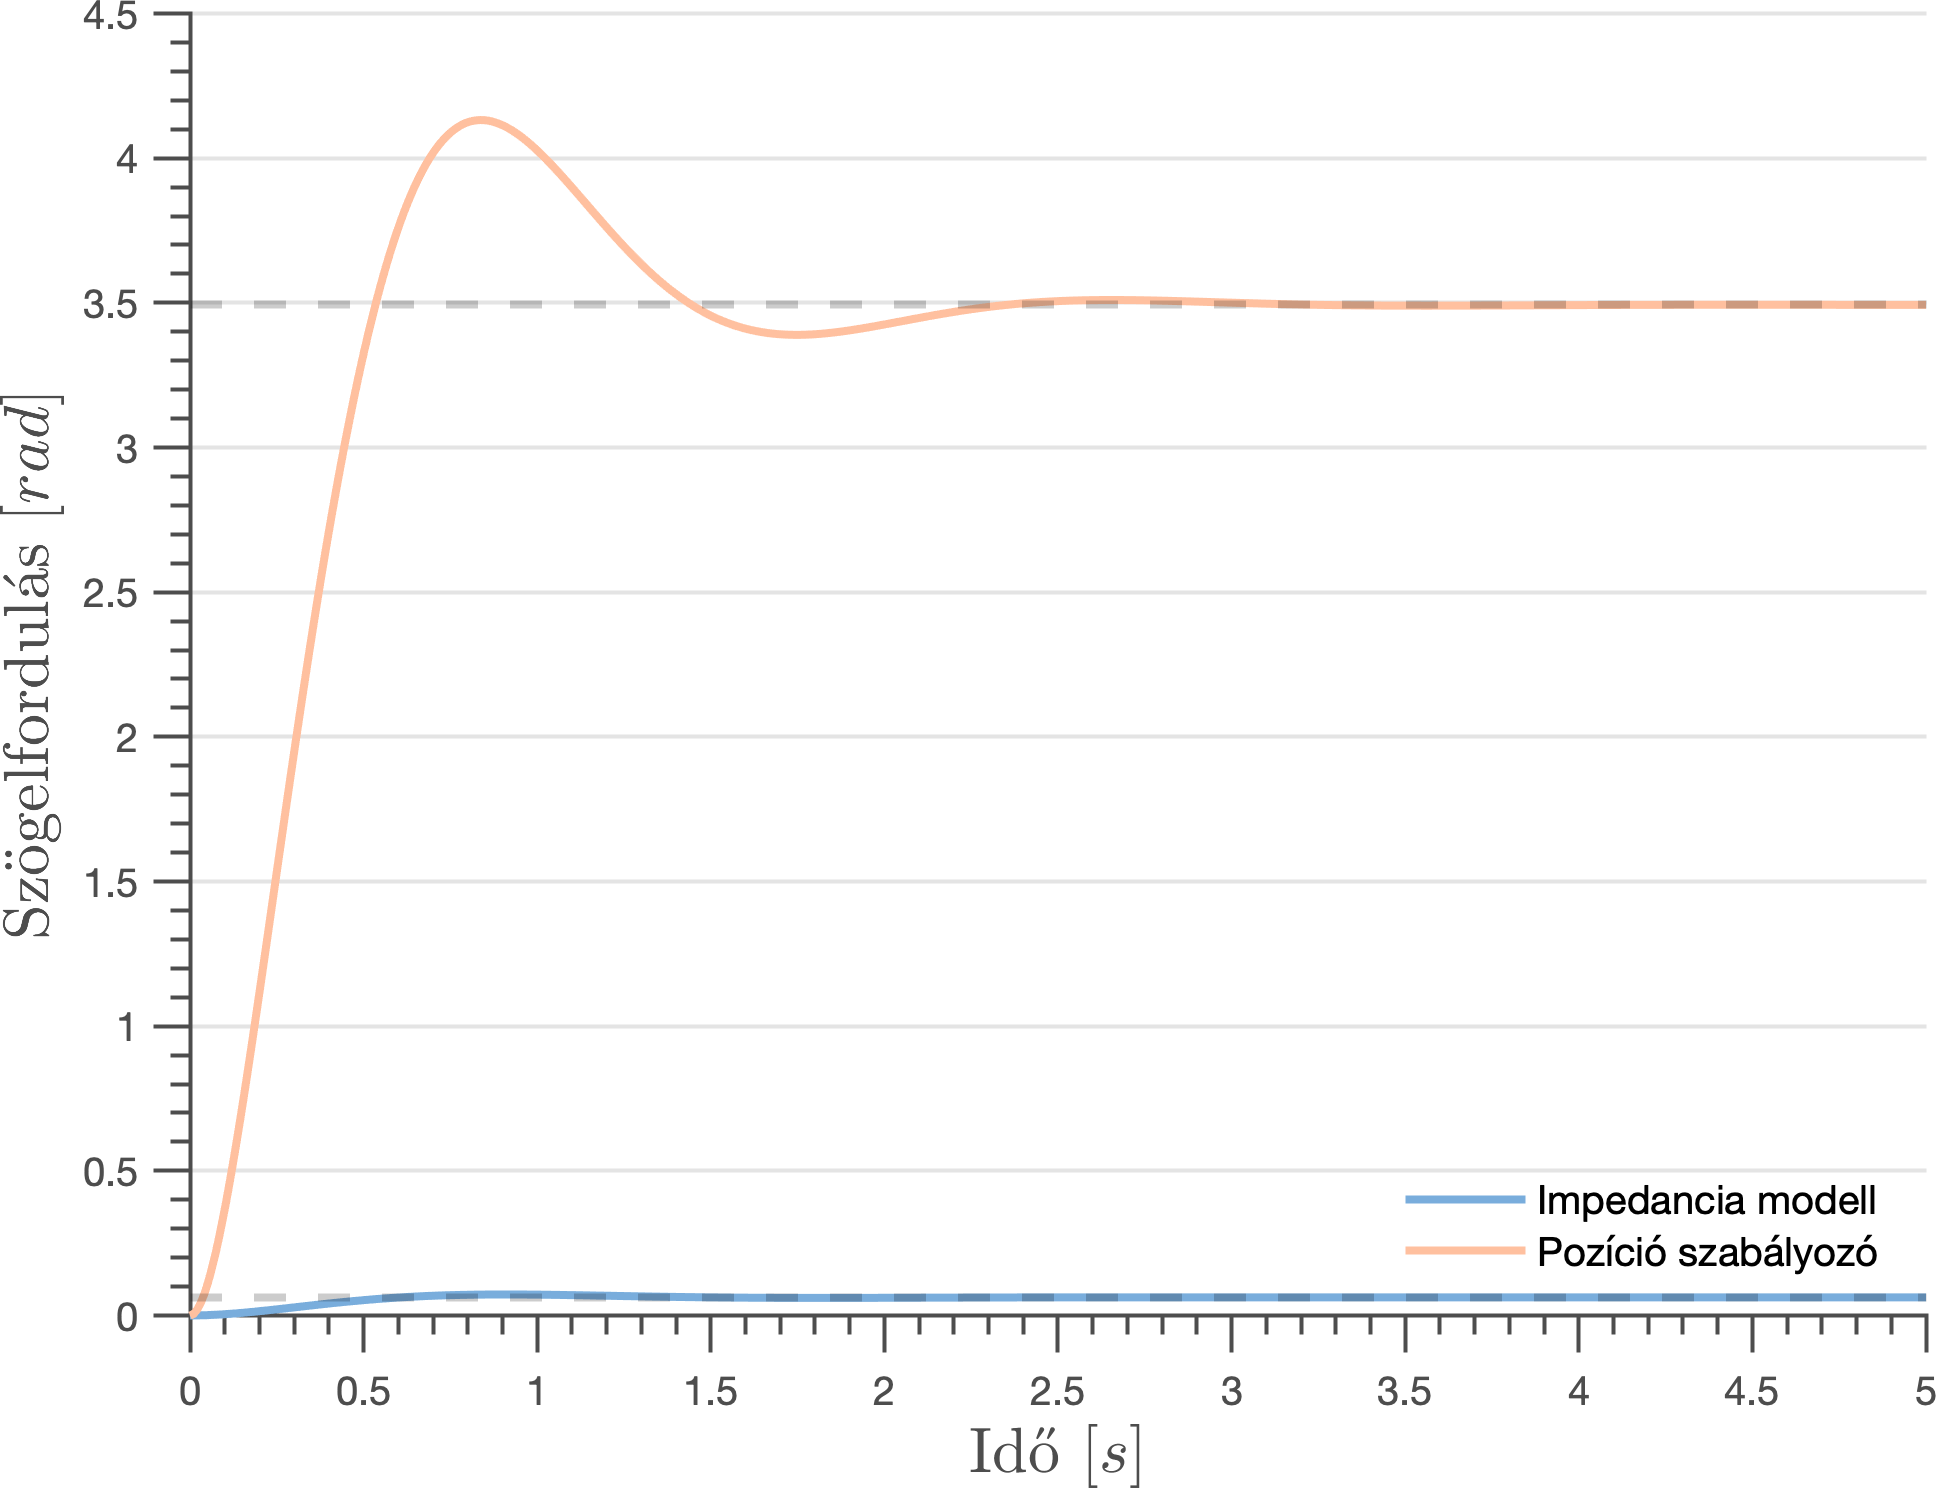
\includegraphics[width=14cm]{images/observer_controller_torque_resp.png}
    \caption{Az impedanciamodell és a szabályozó összehasonlítása külső nyomaték egységugrás bemenetre}\label{fig:observer_controller_torque_resp}
    \end{center}
\end{figure}

A többi pólus meghatározásához szükséges feltételek vizsgálata a nyomatékválasz korrigálása után következik.
A pólusok alapján a visszacsatolási mátrixok az Ackermann formulával lettek meghatározva.

\section{Nyomaték kompenzáció}
A rendszer válasza a külső nyomaték bemenetre adott egységugrás jelre a~\ref{fig:observer_controller_torque_resp}. ábrán látható. 
Az alkalmazott paraméterek a~\ref{tab:observer_controller_pos_resp}. táblázatban szerepelnek.
A végérték nem egyezik meg az impedanciamodell által előírt értékkel, így további módosításokra van szükség.
A modell két bemenete közül csak a feszültségre van hatással a 
szabályozó, így a környezet által kifejtett külső nyomaték 
hatását is a feszültség megváltoztatásával kell kompenzálni. A kompenzáció többek között 
a külső nyomaték direkt vagy indirekt visszacsatolásával érhető el.
Direkt mérés esetén a külső nyomaték értékét egy szenzor adja meg.
A további vizsgálatok során feltételezett, hogy a szenzor dinamikája elhanyagolhatónak tekinthető. Az
állapotmegfigyelővel és kompenzációval ellátott rendszer teljes 
blokkdiagramját a~\ref{fig:block_diagram_direct_compensation}. ábra mutatja.
\begin{figure}[ht]
    \begin{center}
    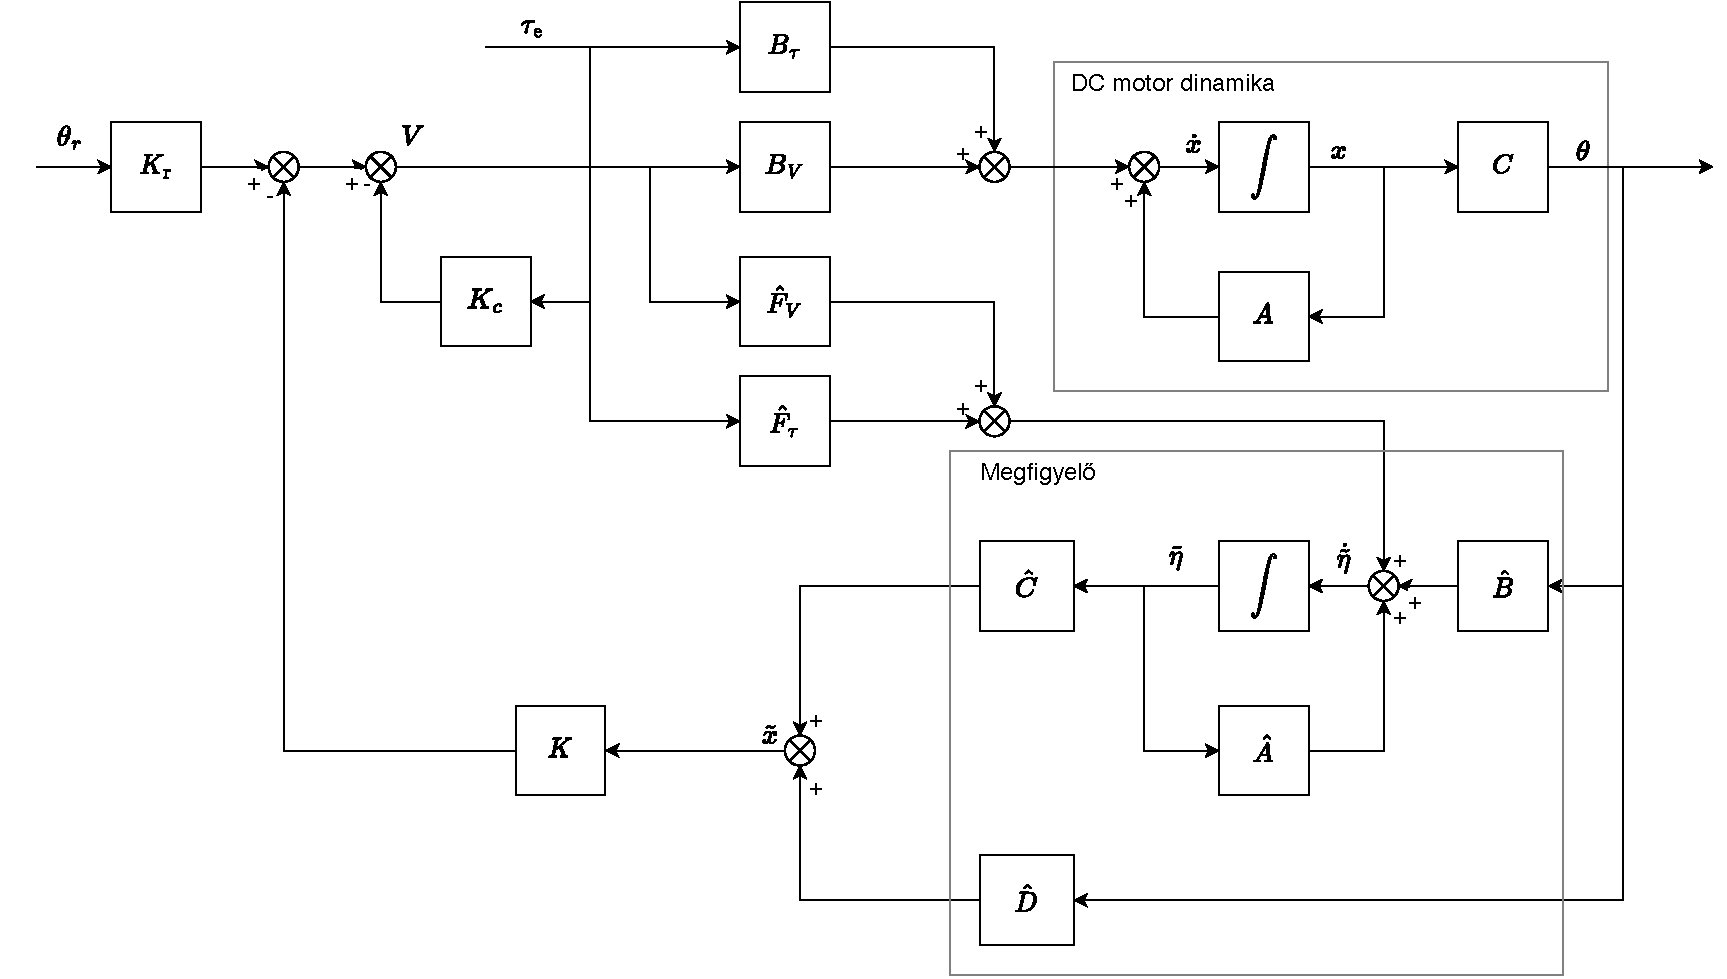
\includegraphics[width=\textwidth]{images/compensated_position_control_torque.pdf}
    \caption{Impedancia szabályozó közvetlen nyomaték méréssel}\label{fig:block_diagram_direct_compensation}
    \end{center}
\end{figure}

A kompenzált rendszernél alkalmazott visszacsatolási összefüggés a~\eqref{eq:position_control_voltage} egyenlethez
hasonló, azonban megjelenik a mért külső nyomaték:
\begin{align}
    V = K_\RM r \theta_\RM r - K_\RM c \tau_\RM e - \BF K \tilde{\BF x}\,,
\end{align}
ahol $\BF K$ az állapot visszacsatolási mátrix, $K_\RM c$ a nyomaték kompenzációs együttható,
$K_\RM r$ a bemeneti erősítési tényezője és $\theta_\RM r$ az előírt szögelfordulás.
A pozíció szabályozónál alkalmazott levezetéshez hasonlóan meghatározható a módosított rendszer teljes dinamikája.
A visszacsatolási összefüggést behelyettesítve az~\eqref{eq:state_space_generic} egyenletbe az
\begin{align}\label{eq:state_control_law_subs}
    \dot{\BF x} = \BF A \BF x + \BF B_\RM V\left[-\BF K \tilde{\BF x} -K_\RM c \tau + K_\RM r \theta_\RM r\right] + \BF B_\RM \tau \tau\,
\end{align}
összefüggés adódik, mely a becsült és a valódi állapotok közötti hibával kifejezve az
\begin{align}
    \dot{\BF x} = \left(\BF A - \BF B_\RM V \BF K\right) \BF x + 
    \BF B_\RM V \BF K \BF e + 
    \left(\BF B_\RM \tau - \BF B_\RM V K_\RM c\right) \tau + 
    \BF B_\RM V K_\RM r \theta_\RM r
\end{align}
alakra hozható. 
A megfigyelő bemenetét kiegészítve a mért külső nyomatékkal az
\begin{equation}
    \begin{split}
    \dot{\BF x}_\RM b &= \BF A_\RM{ba} x_\RM a + \BF A_\RM{bb} \BF x_\RM b + 
    \BF B_\RM{Vb} V + \BF B_\RM{\tau b} \tau_\RM e\,,\\
    \dot{\tilde{\BF x}}_\RM b &= \left(\BF A_\RM{bb} - \BF K_\RM e \BF A_\RM{ab}\right) \tilde{\BF x}_\RM b +
    \BF A_\RM{ba} x_\RM a +
    \BF K_\RM e \BF A_\RM{ab} \BF x_\RM b +
    \BF B_\RM{Vb} V + \BF B_\RM{\tau b} \tau_\RM e\,
    \end{split}
\end{equation}
egyenleteket kapjuk, melyeket kivonva egymásból az \(\BF e\) hibára vonatkozó összefüggéshez jutunk, ami ez esetben:
\begin{align}
    \dot{\BF e} = \left(\BF A_\RM{bb} - \BF K_\RM e \BF A_\RM{ab}\right) \BF e\,.
\end{align}
A rendszer dinamikája blokk mátrix alakban pedig a következő:
\begin{align}
    \begin{bmatrix}
        \dot{\BF x} \\
        \dot{\BF e}
    \end{bmatrix}
    =
    \begin{bmatrix}
        \BF A - \BF B_\RM V \BF K & \BF B_\RM V \BF K_\RM b \\
        \BF 0 & \BF A_\RM{bb} - \BF K_\RM e \BF A_\RM{ab}
    \end{bmatrix}
    \begin{bmatrix}
        \BF x \\
        \BF e
    \end{bmatrix}
    +
    \begin{bmatrix}
        \BF B_\RM \tau - \BF B_\RM V K_\RM c & \BF B_\RM V K_\RM r\\
        \BF 0 & \BF 0
    \end{bmatrix}
    \begin{bmatrix}
        \tau_\RM e \\
        \theta_\RM r
    \end{bmatrix}.
\end{align}

A megfigyelő belső hibájának megváltozása már csak a pillanatnyi belső hibától függ. A \(\BF K_\RM e\) mátrixot 
megfelelően kiválasztva a rendszer belső hibáját tekintve exponenciálisan stabil. Mivel a rendszer teljesen irányítható,
a \(\BF K\) visszacsatolási mátrixot megfelelően kiválasztva a teljes rendszer is exponenciálisan stabil. Továbbá 
a \(K_\RM c\) nyomaték kompenzációs paraméter segítségével a nyomatékválasz végértéke is beállítható.

Indirekt nyomaték visszacsatolás kontextusában (a rendszer szöggyorsulásának mérése alapján) 
a~\ref{fig:block_diagram_indirect_compensation}. ábra mutatja a teljes blokkdiagramot.
\begin{figure}[ht]
    \begin{center}
    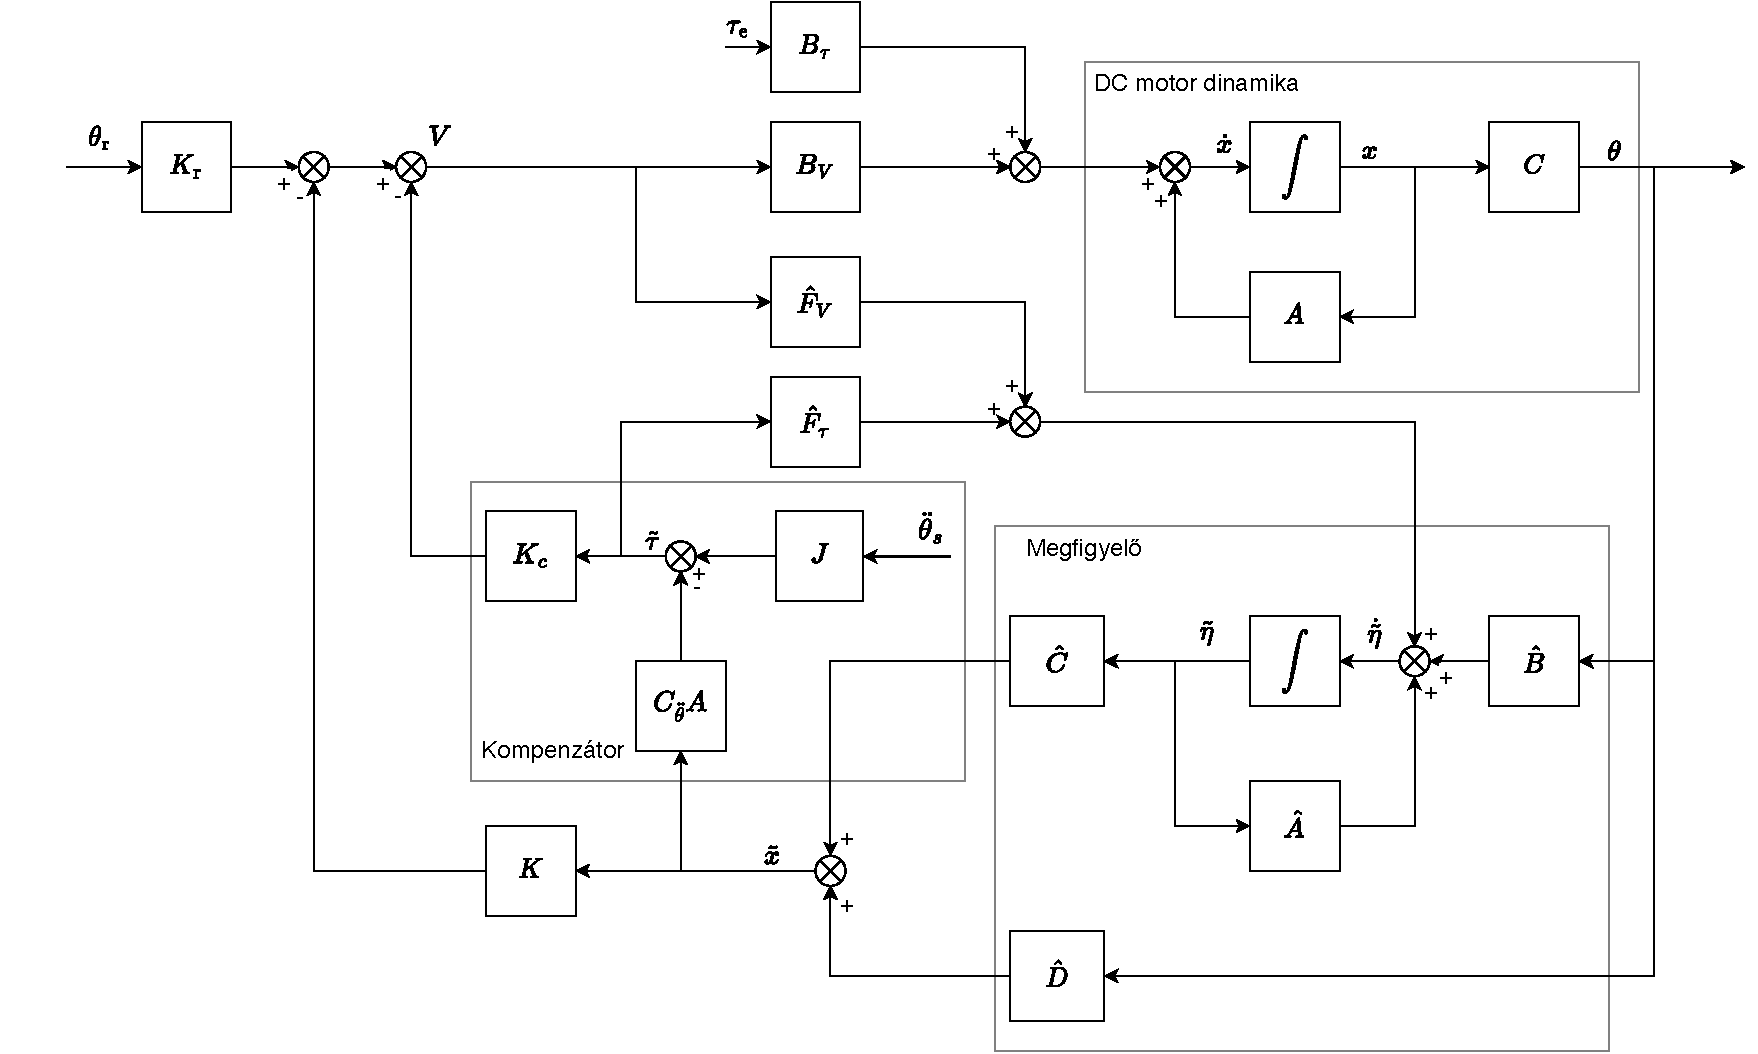
\includegraphics[width=\textwidth]{images/compensated_position_controller_angular_acceleration.pdf}
    \caption{Impedancia szabályozó szöggyorsulás méréssel}\label{fig:block_diagram_indirect_compensation}
    \end{center}
\end{figure}
Ekkor egy becsült nyomaték érték kerül visszacsatolásra:
\begin{align}
    \tilde \tau = J \ddot \theta_\RM s - \BF C_{\ddot\theta} \BF A \tilde{\BF x}\,,
\end{align}
ahol \(\ddot \theta_\RM s\) a forgórész mért szöggyorsulása és \(\BF C_{\ddot\theta} = [0~~1~~0]\),
tehát a becsült állapot és a mért szöggyorsulás lineáris kombinációjával adható meg.
A feszültségjel a becsült nyomatékértékkel:
\begin{align}
    V = K_\RM r \theta_r - K_c \tilde \tau - \BF K \tilde{\BF x}.
\end{align}
Az előző levezetéshez hasonlóan meghatározható a teljes rendszer dinamikája:
\begin{align}
    \begin{bmatrix}
        \dot{\BF x} \\
        \dot{\BF e}
    \end{bmatrix}
    =
    \begin{bmatrix}
        \BF A - \BF B_\RM V \BF K & \BF B_\RM V (\BF K_\RM b - \BF C_{\ddot\theta} \BF A_\RM{*b} K_\RM c) \\
        \BF 0 & \BF A_\RM{bb} - \BF B_\RM{\tau b} \BF C_{\ddot\theta} \BF A_\RM{*b} - \BF K_\RM e \BF A_\RM{ab}
    \end{bmatrix}
    \begin{bmatrix}
        \BF x \\
        \BF e
    \end{bmatrix}
    +
    \begin{bmatrix}
        \BF B_\RM \tau - \BF B_\RM V K_\RM c & \BF B_\RM V K_\RM r\\
        \BF 0 & \BF 0
    \end{bmatrix}
    \begin{bmatrix}
        \tau_\RM e \\
        \theta_\RM r
    \end{bmatrix}.
\end{align}

A megfigyelő visszacsatolási mátrixának kiválasztása valamelyest módosul, de a megfelelő mátrixokkal
a rendszer továbbra is exponenciálisan stabil. Ebben az alkalmazásban direkt mérés alapján kerül meghatározásra
a rendszerre ható külső nyomaték, így a továbbiakban a~\ref{fig:block_diagram_direct_compensation}. ábrán
látható modell vizsgálata fog folytatódni.

A kompenzáció csak akkor lehet eredményes, ha a modellezett motor feszültség és külső nyomaték hatására is 
egyaránt közel azonos sebességgel reagál. Ennek pontos definiálása következik most. A direkt nyomaték méréssel 
kompenzált modell válasza egységugrás bemenetre a~\ref{fig:observer_controller_pos_resp_direct}. 
és~\ref{fig:observer_controller_torque_resp_direct}. ábrán látható. 
A nyomaték jelre adott válasznál a bemenet \(0.1~\RM{Nm}\) nagyságú. A felhasznált paramétereket 
a~\ref{tab:observer_controller_direct_comp_params} táblázat tartalmazza.
\begin{table}[H]
    \small\centering
    \caption{A kompenzált szabályozónál alkalmazott paraméterek}\label{tab:observer_controller_direct_comp_params}
    \tabcolsep=1pt
    \begin{tabular}{l>{~}l>{\quad}rl}
        \toprule
        \multicolumn{2}{c}{Szimbólum és paraméter név} & \multicolumn{2}{c}{Érték} \\ \midrule
        \(M_\RM e\) & Előírt tehetetlenség & \num{1.00e-6} & \(\RM{kg\cdot m^2}\) \\
        \(B_\RM e\) & Előírt viszkózus csillapítás & \num{4.00e-6} & \(\RM{kg\cdot m^2\cdot s^{-1}}\) \\
        \(K_\RM e\) & Előírt rugóállandó & \num{1.60e-5} & \(\RM{kg\cdot m^2\cdot s^{-2}}\) \\
        \(J_\RM a\) & Rotor tehetetlensége & \num{1.44e-7} & \(\RM{kg\cdot m^2}\) \\
        \(J_\RM L\) & Terhelés tehetetlensége & \num{1.00e-4} & \(\RM{kg\cdot m^2}\) \\
        \(J\) & Átszámított tehetetlenség & \num{1.58e-7} & \(\RM{kg\cdot m^2}\) \\
        \(g\) & Áttételi arány & \num{84.3284} & \\
        \(i_\RM{f}\) & Terhelés nélküli állapot állandósult motorárama & \num{4.01e-2} & \(\RM{A}\) \\
        \(\dot{\theta}_\RM{f}\) & Terhelés nélküli állapot állandósult szögsebessége & \num{7.10e2} & \(\RM{rad \cdot s^{-1}}\) \\
        \(B_\RM m\) & Motormodell viszkózus csillapítása & \num{5.64e-5} & \(\RM{kg\cdot m^2\cdot s^{-1}}\) \\
        \(K_\RM m\) & Motor nyomatékállandója & 0.998 & \(\RM{Nm\cdot A^{-1}}\) \\
        \(L\) & Motor induktivitása & 0.452 & H \\
        \(R\) & Motor ellenállása & 10.6 & \(\Omega\) \\
        \bottomrule
    \end{tabular}
\end{table}
A pólusok továbbra is a~\ref{tab:observer_controller_pos_resp}. táblázat után definiált értékek. 
Az paraméterek egy valószerű kísérleti összeállítás motorjának paramétereit 
tartalmazzák. Ez az összeállítás tartalmaz egy fogaskerekes áttételt, így bizonyos paramétereket 
át kell számítani a terhelési oldalról a motor oldalára. A motor viszkózus csillapítása és tehetetlensége származtatott értékek, melyek 
\begin{align}
    \begin{split}
        J &= J_\RM a + \frac{1}{g^2}J_\RM L\,, \\
        B_\RM m &= \frac{K_\RM m i_\RM{f}}{\dot{\theta}_\RM{f}}\,.
    \end{split}
\end{align}
A nyomaték kompenzációs együttható
\begin{equation}
    K_\RM c = L\frac{- B_\RM m M_\RM e + B_\RM e J - J M_\RM e p + J^2 p}{J K_\RM m M_\RM e}
\end{equation}
összefüggés szerint számolható a végérték tétel alapján a~\eqref{eq:input_gain} egyenlethez hasonlóan.
A pozíció referencia jelre adott válasz változatlan, azonban a külső nyomatékra adott válasz végértéke már
megegyezik az impedanciamodell által előírt értékkel. A válaszban megfigyelhető túllövés kiküszöböléshez
a motor és az impedanciamodell paraméterei, valamint a rendszer válasza közötti kapcsolat további vizsgálata szükséges.

\begin{figure}[ht]
    \begin{center}
    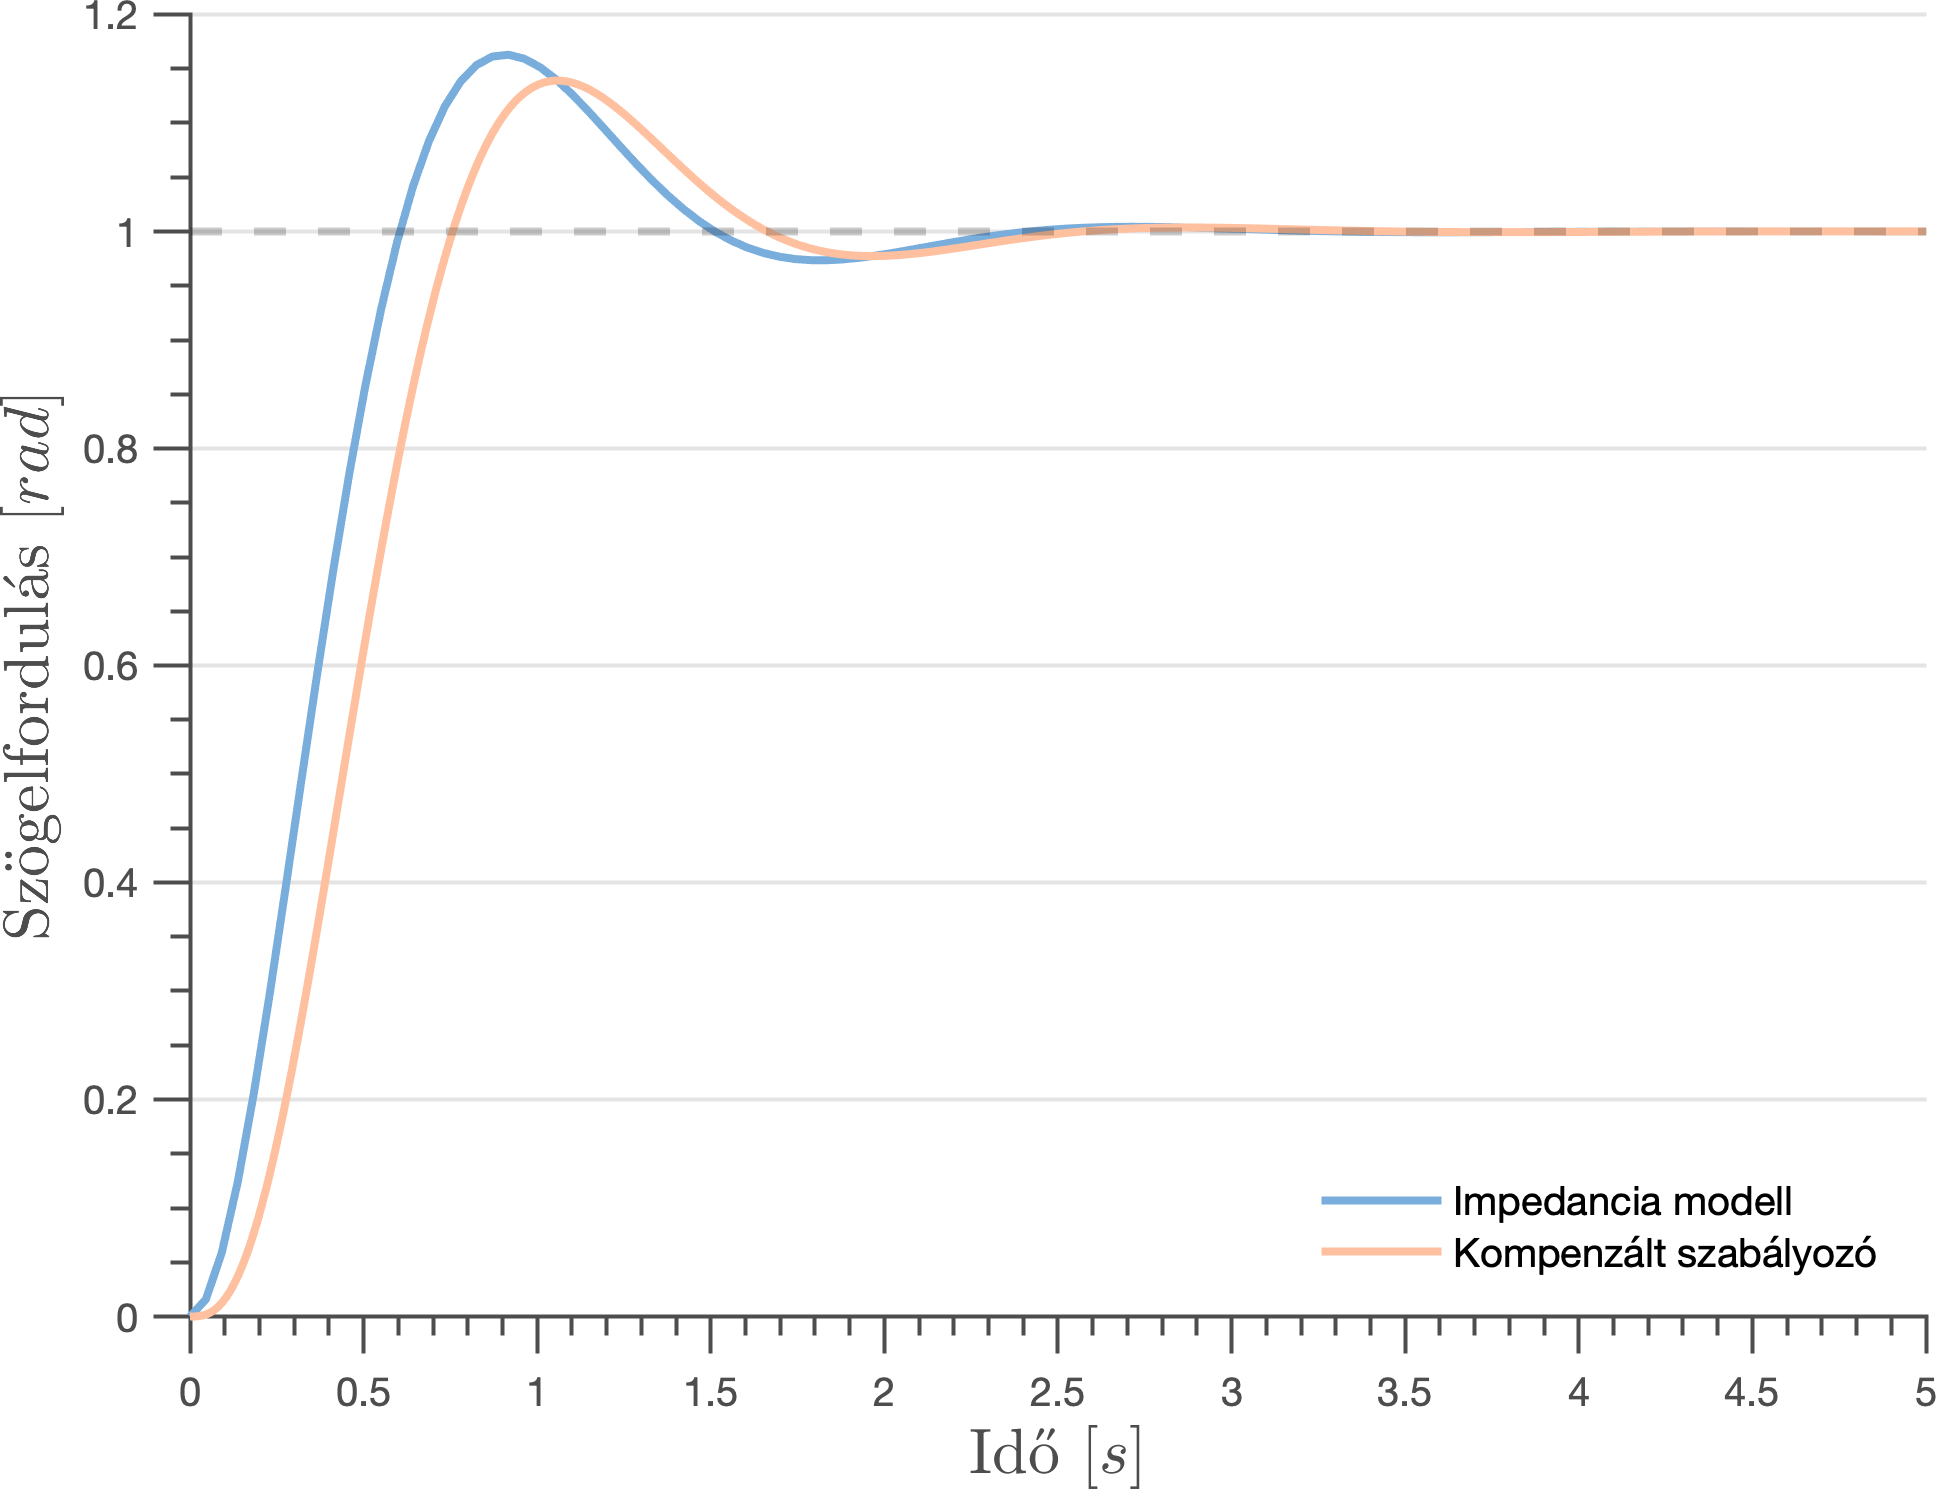
\includegraphics[width=\textwidth]{images/observer_controller_pos_resp_direct_comp.png}
    \caption{Az impedanciamodell és a kompenzált szabályozó összehasonlítása pozíció egységugrás bemenetre}\label{fig:observer_controller_pos_resp_direct}
    \end{center}
\end{figure}

\begin{figure}[ht]
    \begin{center}
    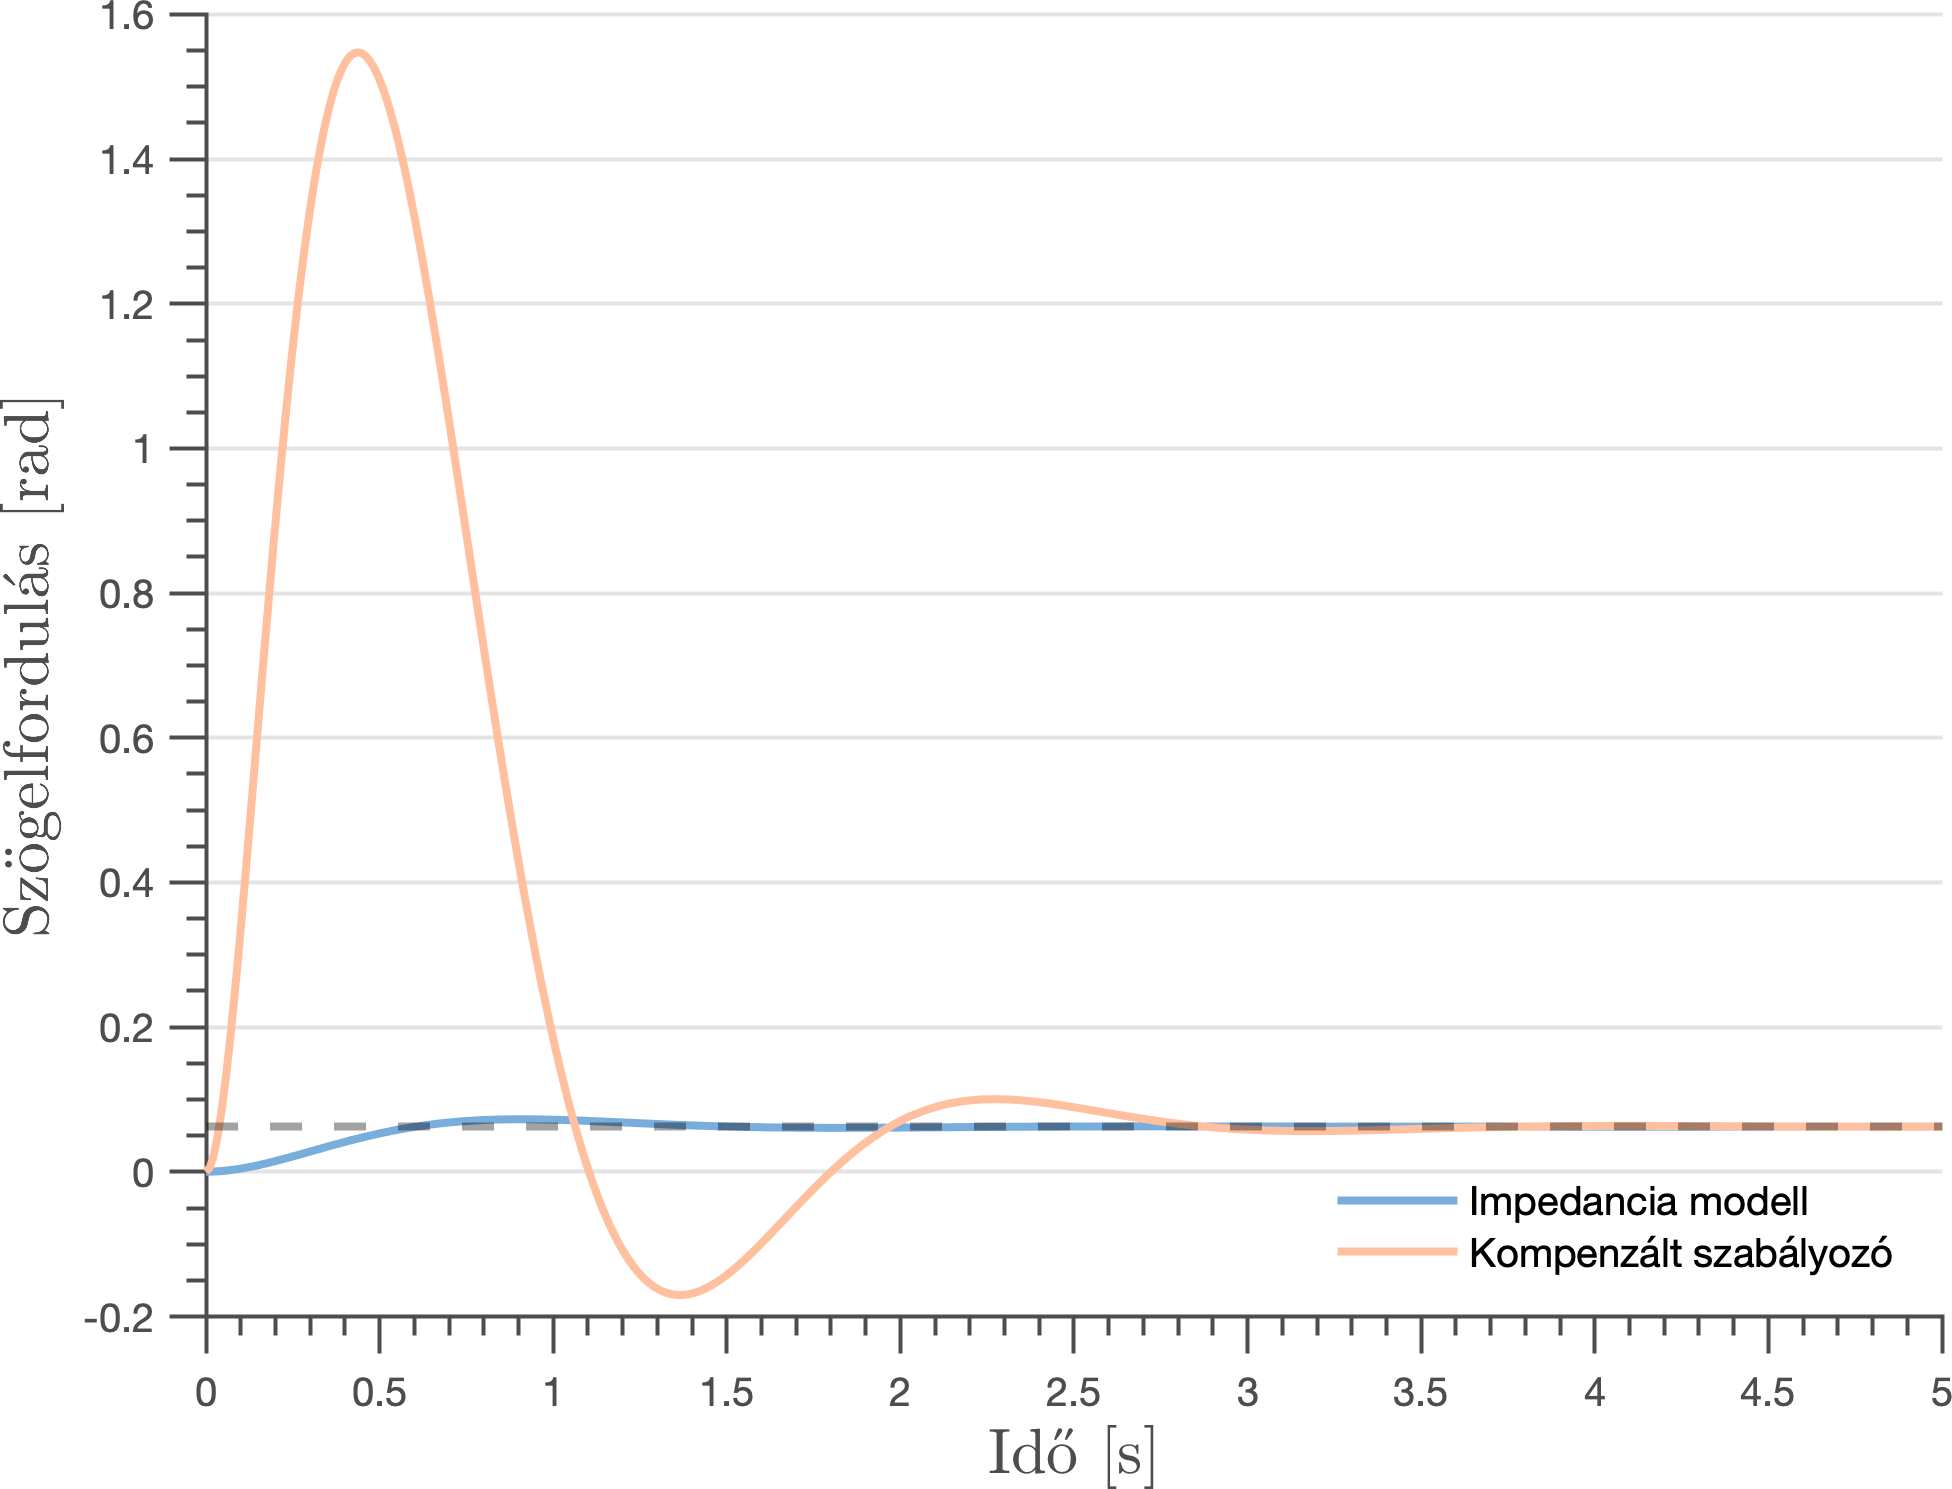
\includegraphics[width=\textwidth]{images/observer_controller_torque_resp_direct_comp.png}
    \caption{Az impedanciamodell és a kompenzált szabályozó összehasonlítása külső nyomaték egységugrás bemenetre}\label{fig:observer_controller_torque_resp_direct}
    \end{center}
\end{figure}

Először is az impedanciamodell paraméterei mind valós pozitív értékkel kell rendelkezzenek, enélkül a rendszer 
azonnal instabil lesz. Ez a Routh--Hurwitz kritérium alapján következik az impedanciamodell karakterisztikus egyenletéből.
Az áthelyezett pólusok közül az első kettőt az impedanciamodell előírt értékei határozzák meg. 
A harmadik áthelyezett pólus, illetve a megfigyelő pólusai függetlenek. A független pólusok meghatározásához 
mindegyik azonos lesz és valós értékű. Ha a pólusok túl közel helyezkednek el az impedanciamodell pólusaihoz,
esetleg még a képzetes tengelyhez is közelebb vannak, akkor eltorzítják a választ. Ha túl nagy negatív valós
értékkel rendelkeznek, az a szabályozó kimenetének szaturációjához vezet, illetve magát a szabályozót is
instabillá teszik. Ennek elkerülése érdekében a lehető legkisebb abszolút értékű negatív valós pólus használata a cél. 
A rendszer átviteli függvénye a pozíció referencia jelet tekintve~\eqref{eq:input_coeff} felhasználásával:
\begin{align}
    \frac{\theta(s)}{\theta_\RM r (s)} = \frac{K_\RM e p}{(p-s)(M_\RM e s^2 + B_\RM e s + K_\RM e)}\,,
\end{align}
ahol \(p\) a keresett szabadon választható pólus. A pólus hatása közelíthető egy időkéséses taggal, mivel
\begin{align}
    e^{-\tau s} = 1 - \tau s + \cdots\,,
\end{align}
ahol \(\tau\) az időkésés. Fontos megjegyezni, hogy ez a közelítés csak \(p \gg 1\) esetben alkalmazható. 
Az átviteli függvény a következő késleltetett másodrendű rendszerrel közelíthető:
\begin{align}
    \frac{\theta(s)}{\theta_\RM r (s)} \approx \frac{K_\RM e}{M_\RM e s^2 + B_\RM e s + K_\RM e}e^{\frac{1}{p}s}\,,
\end{align}
tehát \(\tau = -\frac{1}{p}\) felhasználható a pólus maximumának meghatározásához. A továbbiakban 
ez az időkésés a rendszer beállási idejének legfeljebb 5\%-ára lesz korlátozva. Eszerint a pólus legfeljebb:
\begin{align}\label{eq:pole_selection_pos}
    p_\RM{max} = -\frac{1}{\frac{4}{\zeta \omega_0} \cdot 0.05} = -\frac{B_\RM e}{8M_\RM e \cdot 0.05}
\end{align}
lesz. A külső nyomatékra adott válasz időtartománybeli vizsgálata további feltételekhez vezet. 
Nem minden paraméterkombináció ad elfogadható választ, ahogy a~\ref{fig:observer_controller_torque_resp_direct}.
ábrán is látszik. A rendszer átviteli függvénye a külső nyomaték jelet tekintve:
\begin{align}
    \frac{\theta(s)}{\tau_\RM e (s)} = 
    \frac{Jp - M_\RM e s}{J(p-s)(M_\RM e s^2 + B_\RM e s + K_\RM e)} = 
    \frac{1 -\frac{M_\RM e}{Jp} s}{(1-\frac{1}{p}s)(M_\RM e s^2 + B_\RM e s + K_\RM e)}\,.
\end{align}
Hasonlóan az előző feltételhez a függvény közelíthető egy késleltetett másodrendű rendszerrel. A válaszban 
megjelenik a bemenet deriváltja. A derivált tag hatásának korlátozása ad újabb maximumot a független pólusok értékére. A 
továbbiakban a bemeneti jel deriváltjának együtthatója legalább egy nagyságrenddel kisebb kell legyen egynél.
Ebből következik, hogy a pólus értékének maximuma:
\begin{align}\label{eq:pole_selection_torque}
    p_\RM{max} = -10 \cdot \frac{M_\RM e}{J}
\end{align}
A két feltétel együtt azt eredményezi, hogy a pólus értéke abszolút értékben a lehető legkisebb, amikor
az előírt tehetetlenség és a pólus értékének maximuma:
\begin{equation}\label{eq:pole_selection_extremum}
    \begin{split}
        M'_\RM e &= 0.5 \cdot \sqrt{JB_\RM e}\,, \\
        p'_\RM{max} &= -5 \cdot \sqrt{\frac{B_\RM e}{J}}\,.
    \end{split}
\end{equation}
A szaturáció elkerüléséhez szükséges feltételek részletes vizsgálata túlmutat ezen a dolgozaton, azonban feltételezhetően 
a pólusválasztásnál van egy minimum érték, mely alatt a rendszer nem képes követni az impedanciamodellt. Jelölje \(p_\RM{min}\) ezt a 
minimumot. Ekkor az előírt tehetetlenség lehetséges értékei a~\eqref{eq:pole_selection_pos} és a~\eqref{eq:pole_selection_torque} 
egyenletekben szereplő feltételek szerint egy adott intervallumra korlátozódnak:
\begin{align}
    -\frac{B_\RM e}{8p_\RM{min} \cdot 0.05} < M_\RM e < -0.1 \cdot Jp_\RM{min}\,,
\end{align}
illetve az előírt viszkózus csillapítási együtthatóra is adódik egy maximális korlát~\eqref{eq:pole_selection_extremum} alapján:
\begin{align}
    B_\RM{e,max} = 0.04 \cdot Jp^2_\RM{min}\,,
\end{align}
ami felett nem választható ki olyan pólus, mely a követelményeknek megfelelő választ eredményez. 
\begin{figure}[b!]
	\begin{center}
		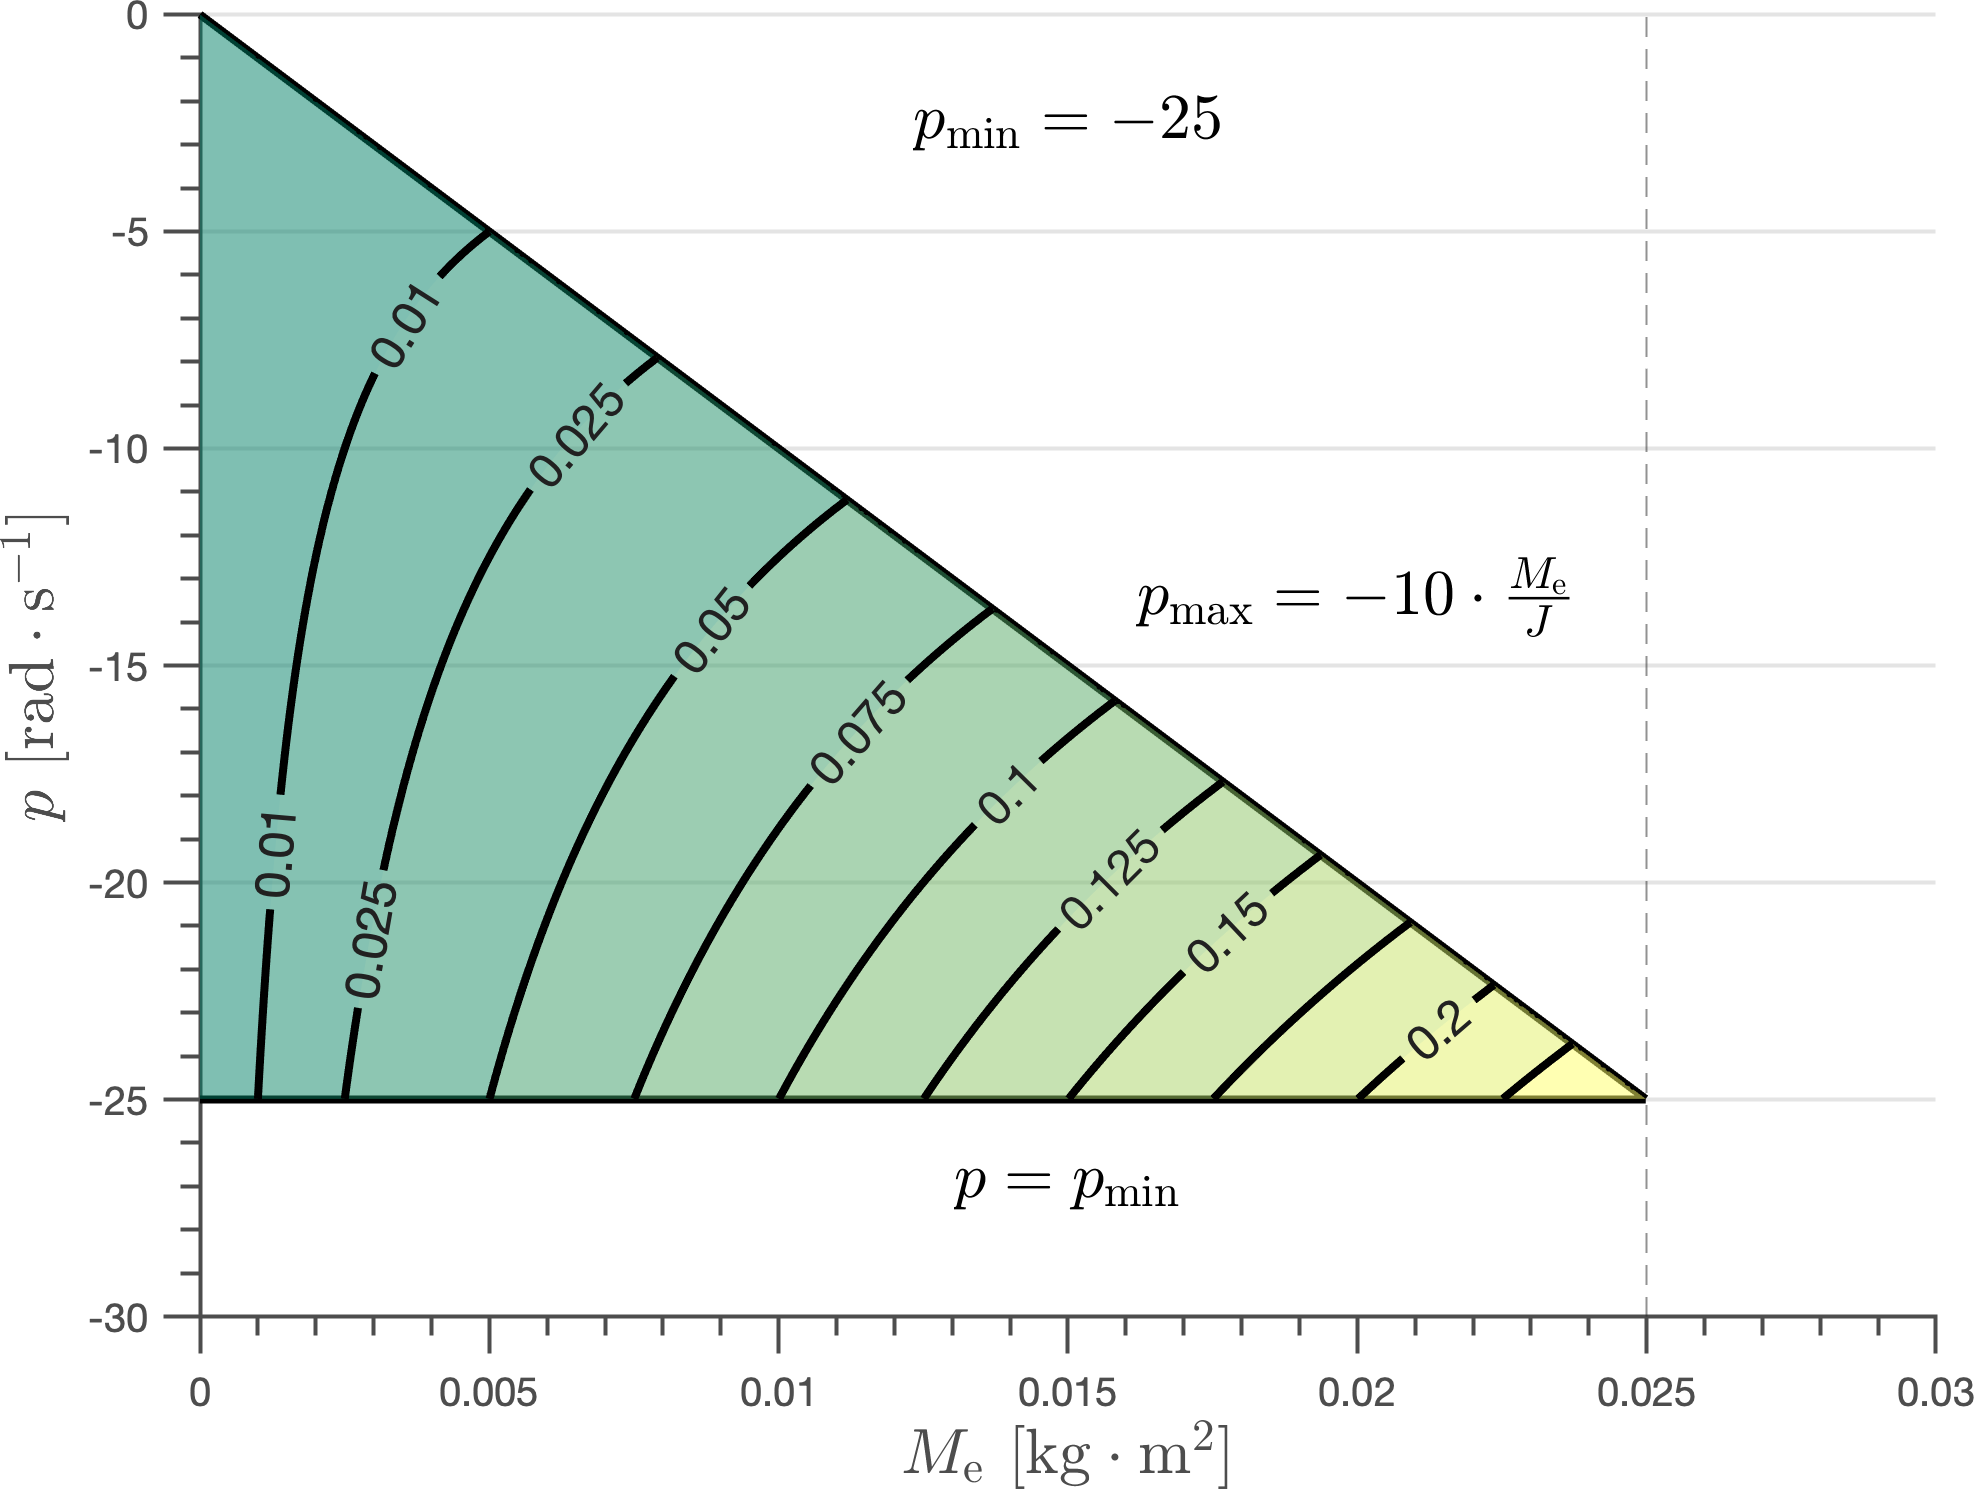
\includegraphics[height=0.5\textheight]{images/observer_controller_param_limits.png}
		\caption{Az előírható tehetetlenség és a független pólus közötti összefüggés}\label{fig:observer_controller_param_limits}
	\end{center}
\end{figure}
Egy adott \(p_\RM{min}\) minimum pólus értékre és \(J\) motor tehetetlenségre ábrázolja 
a választható tehetetlenség - pólus párokat a~\ref{fig:observer_controller_param_limits}. ábra.
A kontúrok konstans normalizált \(\frac{B_\RM e}{J}\) előírt viszkózus csillapítási tényezőket jelölnek a~\eqref{eq:pole_selection_pos}
egyenlet szerint.



Az előző feltételek alapján a pozíció referencia jelre és külső nyomaték hatására is megfelelő válasz kapható.
Egy ilyen válasz látható a~\ref{fig:observer_controller_pos_resp_direct_calib}. 
és a~\ref{fig:observer_controller_torque_resp_direct_calib}. ábrán. 
A módosított impedanciamodell paramétereket a~\ref{tab:observer_controller_pos_resp_calib}. táblázat tartalmazza.
Az összes többi paraméter továbbra is megegyezik a~\ref{tab:observer_controller_direct_comp_params}. 
táblázatban megtalálható értékekkel. 

\begin{table}[H]
    \small\centering
    \caption{A kalibrált szabályozónál alkalmazott paraméterek}\label{tab:observer_controller_pos_resp_calib}
    \tabcolsep=1pt
    \begin{tabular}{l>{~}l>{\quad}rl}
        \toprule
        \multicolumn{2}{c}{Szimbólum és paraméter név} & \multicolumn{2}{c}{Érték} \\ \midrule
        \(M_\RM e\) & Előírt tehetetlenség (\(2J\)) & \num{3.16e-7} & \(\RM{kg\cdot m^2}\) \\
        \(B_\RM e\) & Előírt viszkózus csillapítás (\(4M_\RM e\)) & \num{1.26e-6} & \(\RM{kg\cdot m^2\cdot s^{-1}}\) \\
        \(K_\RM e\) & Előírt rugóállandó (\(4B_\RM e\)) & \num{5.06e-6} & \(\RM{kg\cdot m^2\cdot s^{-2}}\) \\
        \(p\) & További pólusok & -20 & \(\RM{rad \cdot s^{-1}}\) \\
        \(K_\RM c\) & Nyomaték kompenzációs együttható & -160.83 & \(\RM{V \cdot N^{-1} m^{-1}}\) \\
        \bottomrule
    \end{tabular}
\end{table}

\begin{figure}[!htb]
    \begin{center}
    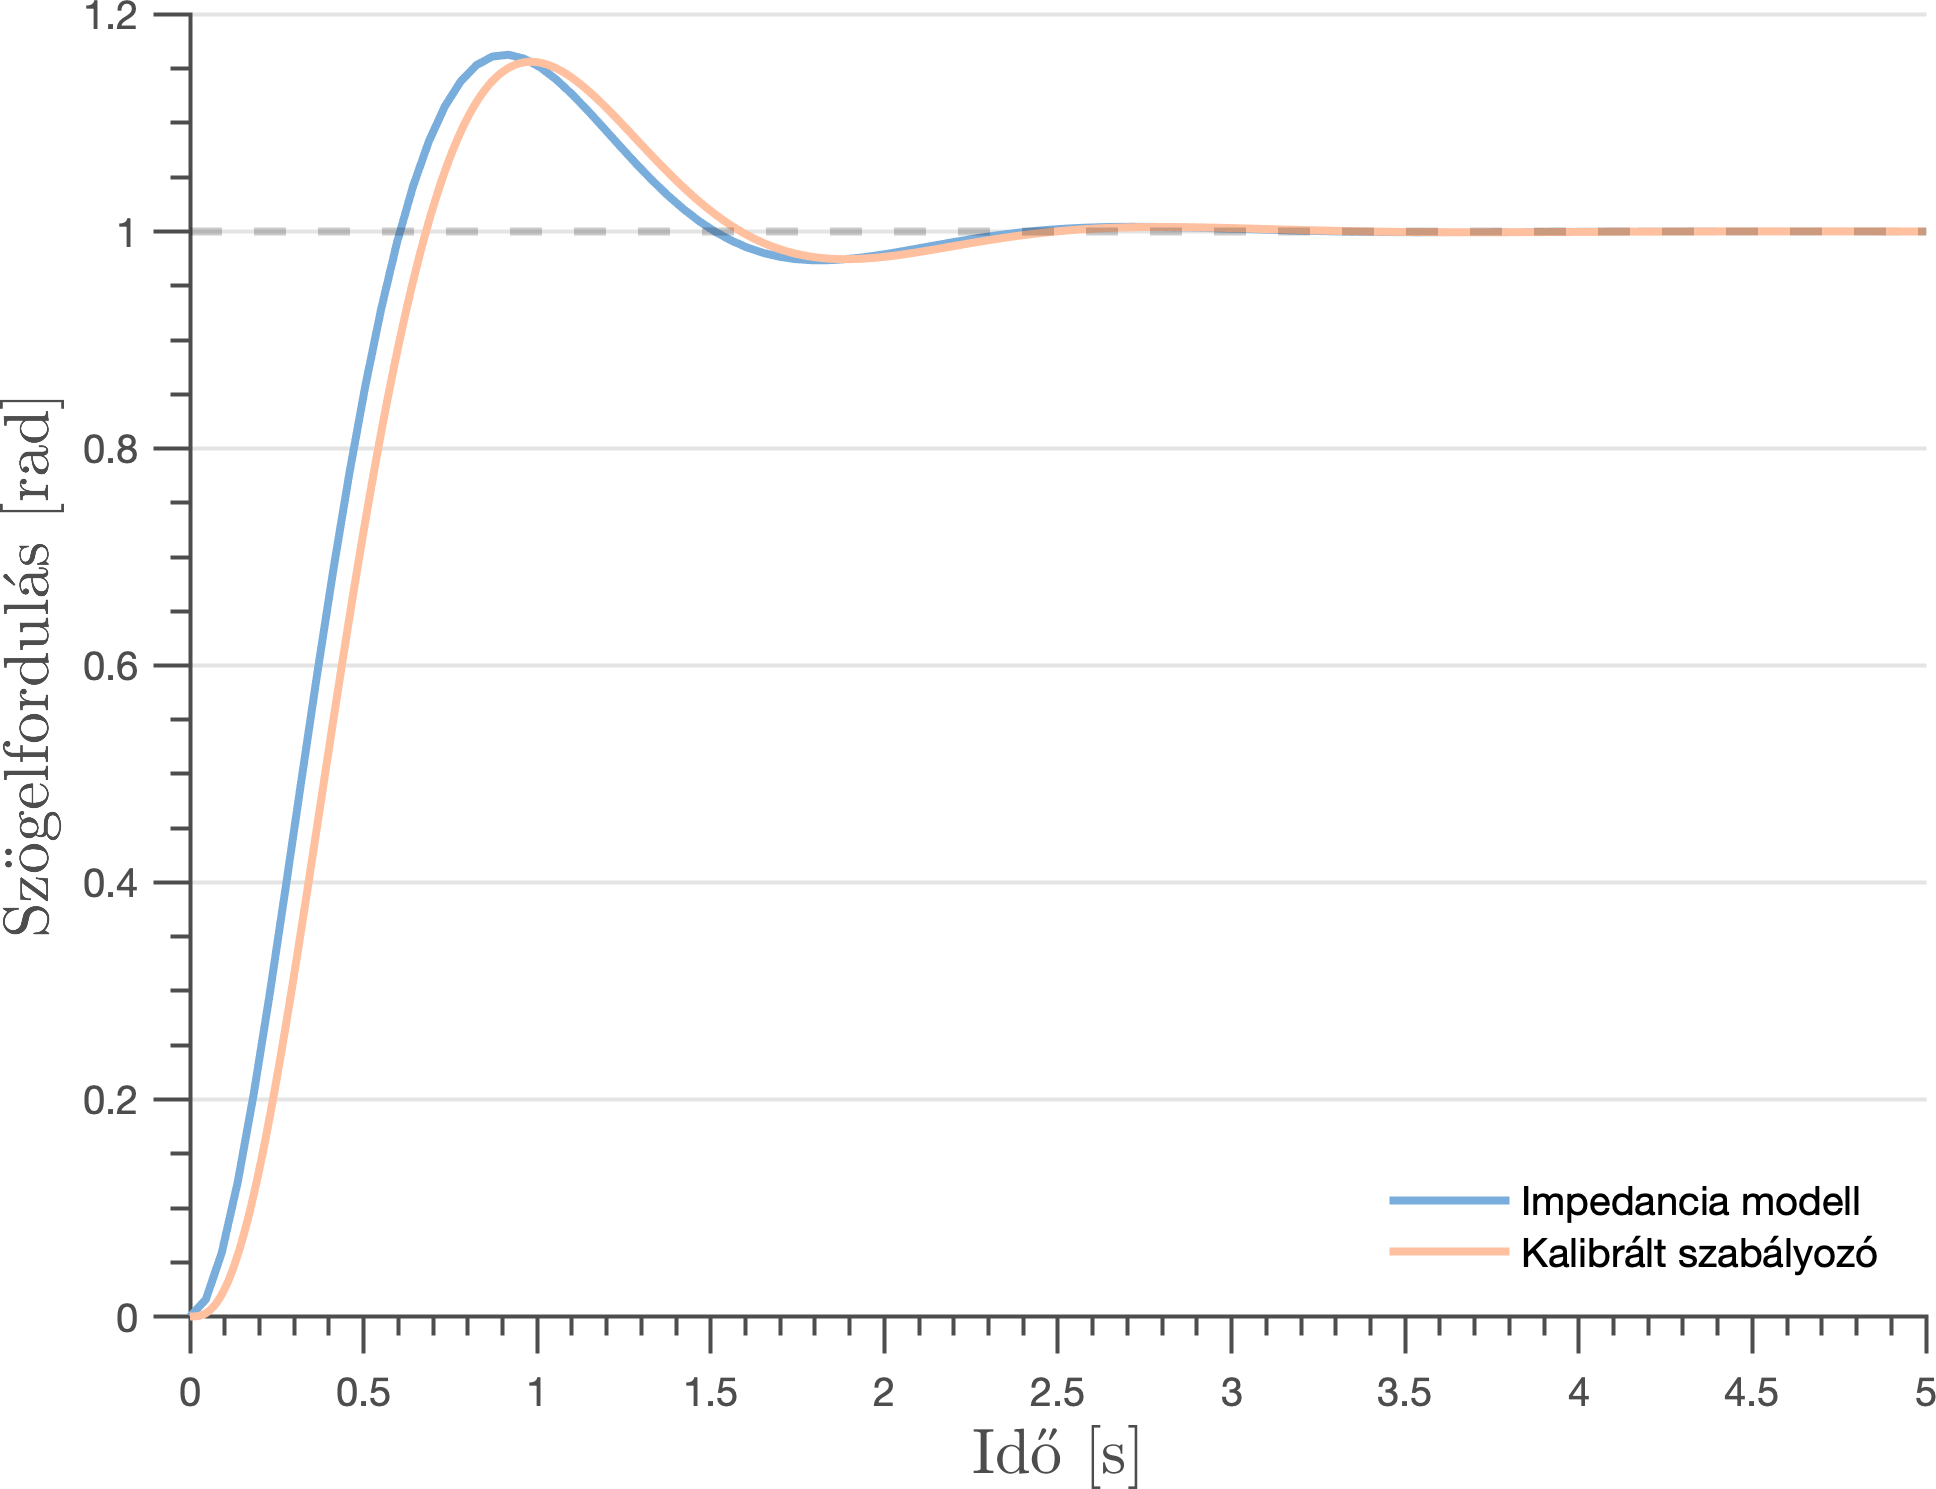
\includegraphics[width=13cm]{images/observer_controller_pos_resp_direct_comp_calib.png}
    \caption{Az impedanciamodell és a kalibrált szabályozó összehasonlítása pozíció egységugrás bemenetre}\label{fig:observer_controller_pos_resp_direct_calib}
    \end{center}
\end{figure}
\begin{figure}[H]
    \begin{center}
    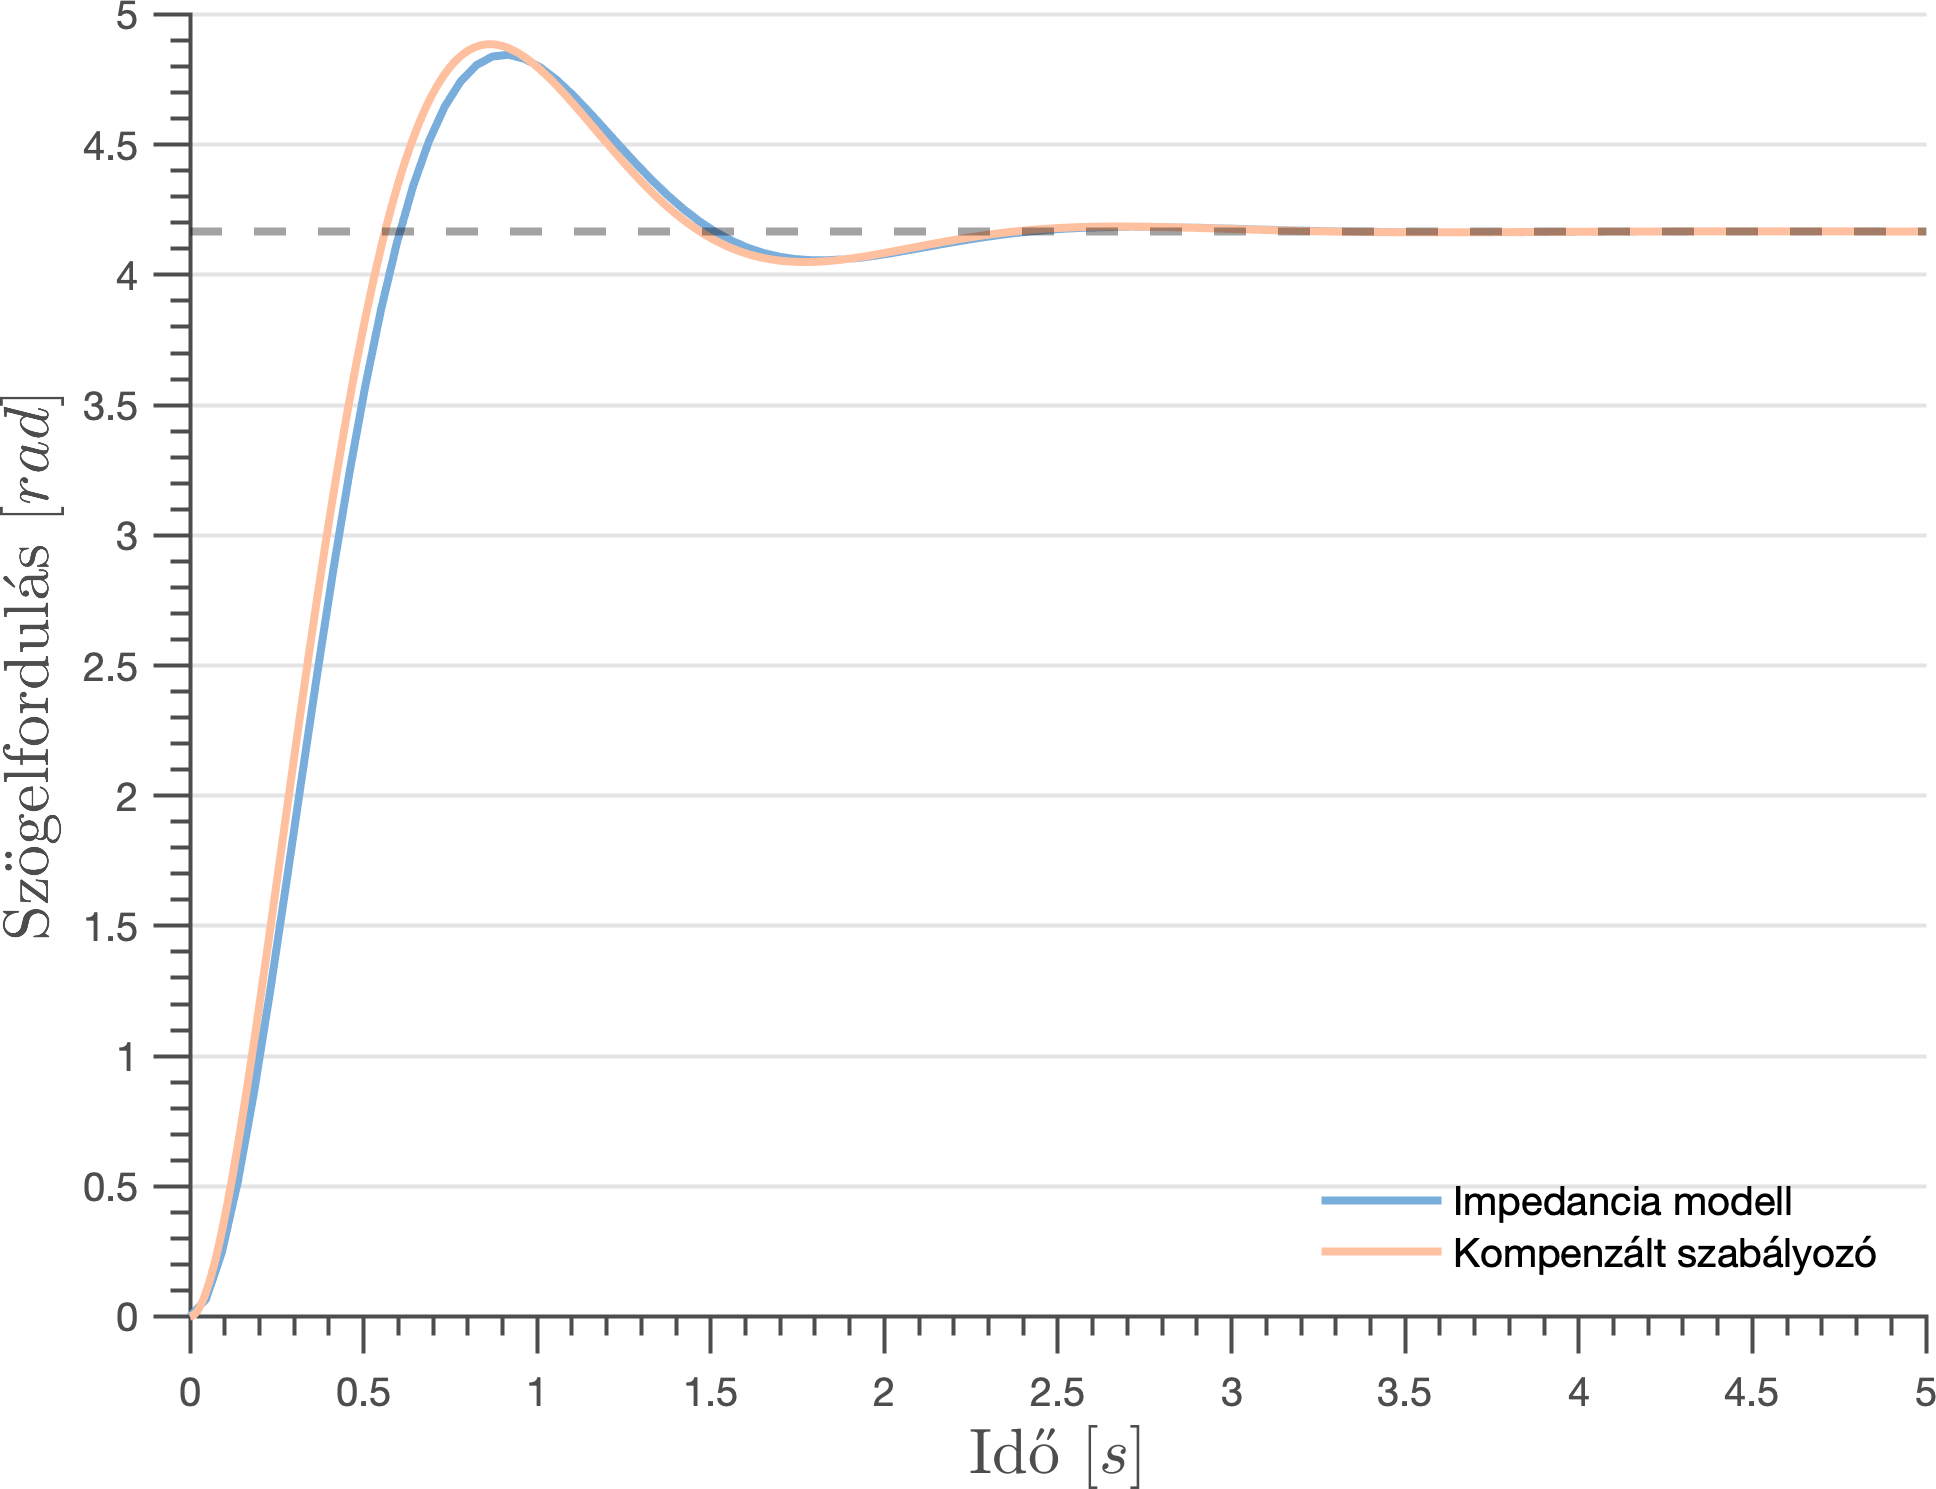
\includegraphics[width=13cm]{images/observer_controller_torque_resp_direct_comp_calib.png}
    \caption{Az impedanciamodell és a kalibrált szabályozó összehasonlítása külső nyomaték egységugrás bemenetre}\label{fig:observer_controller_torque_resp_direct_calib}
    \end{center}
\end{figure}

Az impedanciamodell előírt rugóállandójára az előző elemzés nem ad korlátot, viszont 
ennek a paraméternek a növelésével növekszik a modell sajátfrekvenciája. Ez mindenképp 
egyre nagyobb előírt gyorsulással jár, mely a motorra kapcsolt feszültség szaturációjához vezet.

Az áthelyezett pólusok értékeinek függvényében a szabályozó önmagában instabil lehet. Mivel a rendszer szabályozás 
nélkül instabil, mindenképp szükséges független biztonsági mechanizmus beépítése, így ennek az esetnek az elemzése elmarad. 


\chapter{Stabilitásvizsgálat időkéséssel}\label{chap:time_delay_stability}

A modell és a motor paramétereken kívül a rendszer különböző elemeiben megjelenő időkésés 
is hatással van a stabilitásra. Elegendően nagy időkésés mellett nem csak a mozgásra előírt 
feltételek sérülnek, hanem teljesen instabillá válhat a rendszer. Az időkésés hatását analitikusan egyszerűbb 
rendszereknél például a Lambert-féle W-függvény segítségével~\citep{Yi2012, MatrixLambert2007}, 
vagy D-szeparációval lehet vizsgálni. A Lambert-féle W-függvény bonyolultabb rendszereknél nehezen 
vagy egyaltalán nem alkalmazható~\citep{CepedaGomez2015}, így a következő fejezetben a D-szeparáció módszere 
kerül alkalmazásra.

\section{Stabilitás folytonos időben}

Időkésés megjelenhet a rendszer különböző pontjain. A motor kimenetének mérése, az adatáramlás 
a szabályozó részegységei között és a szabályozó jel kiszámítása mind időt vesznek igénybe. 
Ezeknek a hatásoknak az összeségét egy konstans átlag időkésés reprezentálja. A továbbiakban ez a 
paraméter legyen \(\tau_\RM d\).
\begin{figure}[ht]
    \begin{center}
    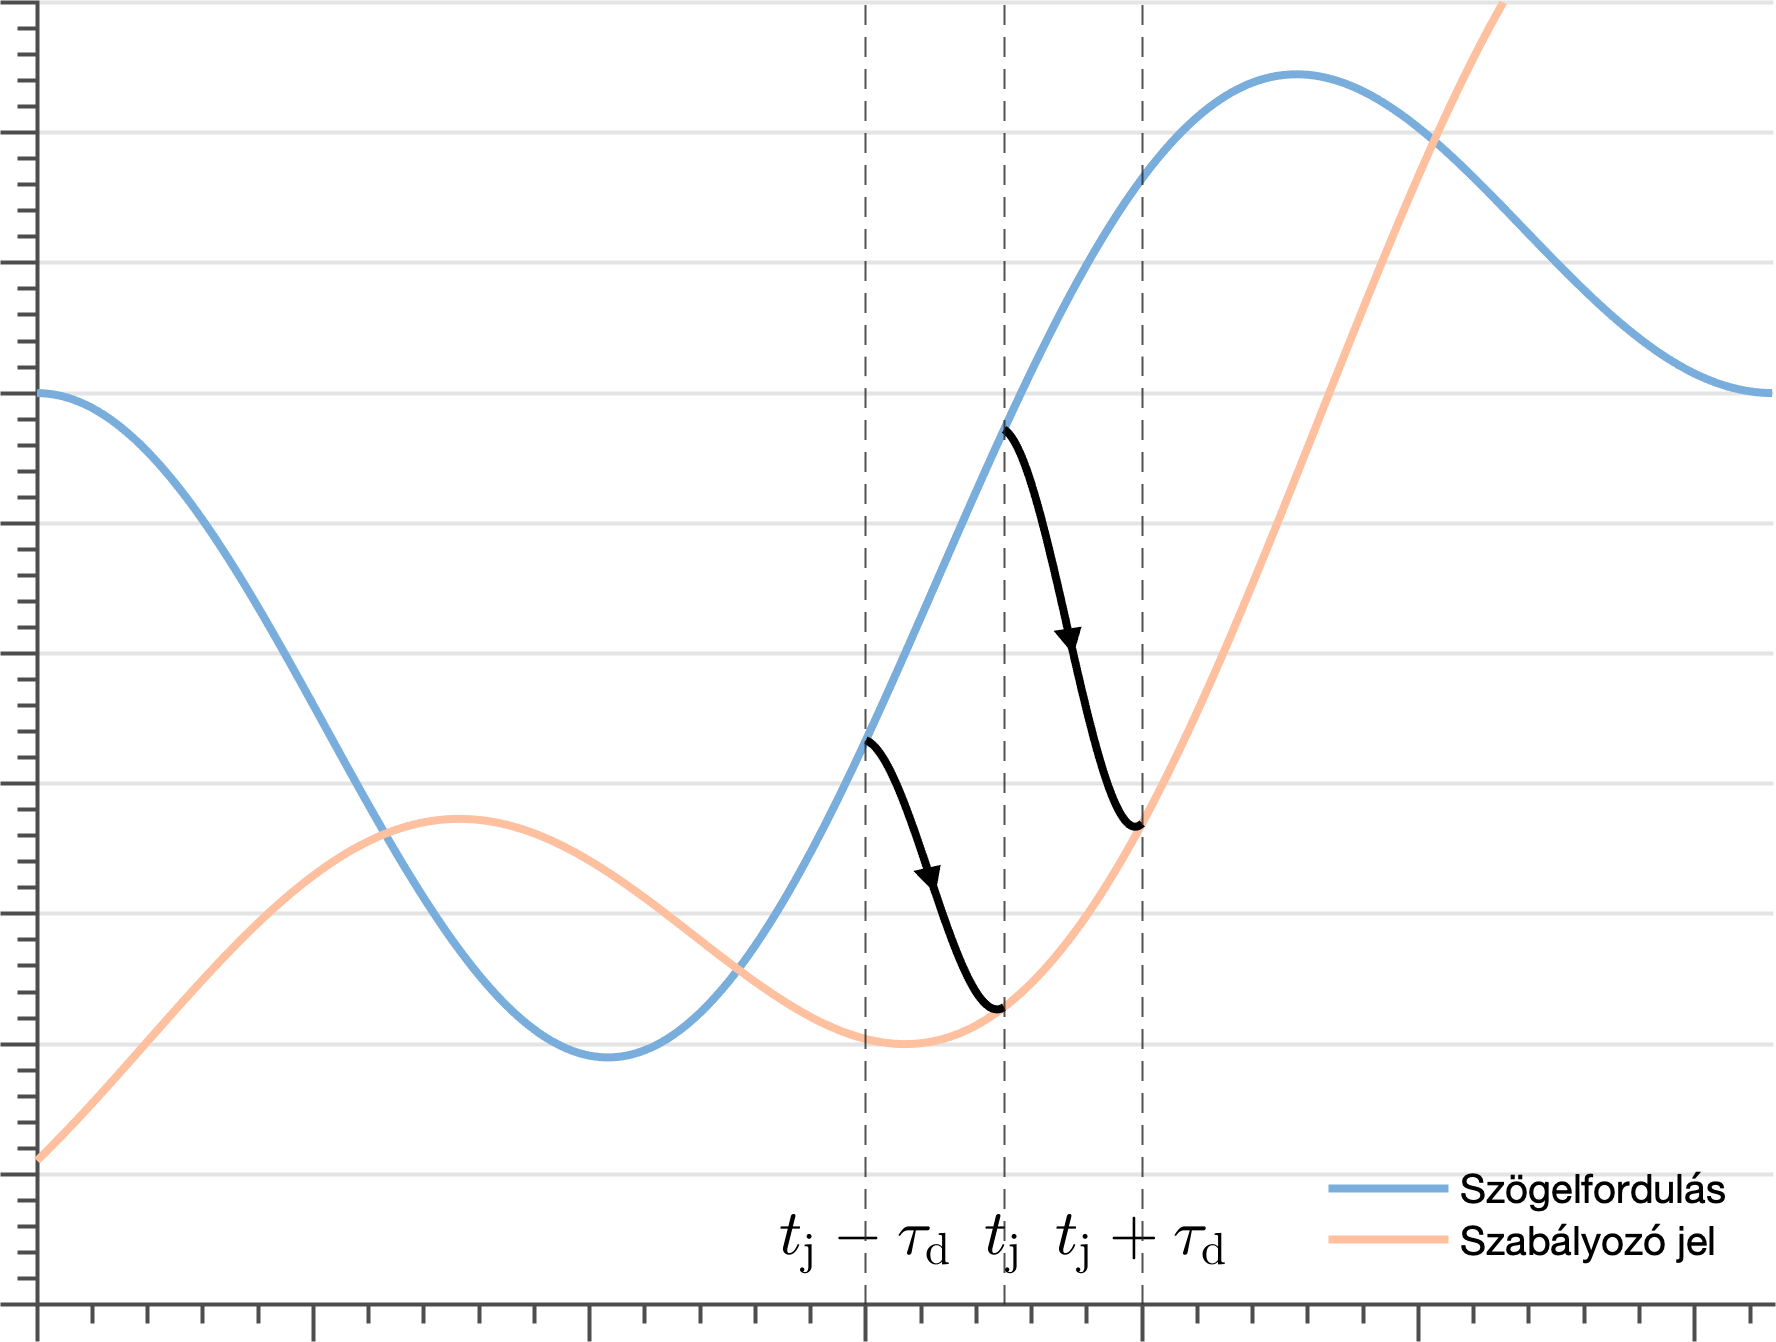
\includegraphics[width=12cm]{images/time_delay_example.png}
    \caption{Reprezentatív ábra az időkésés hatásáról folytonos időben}\label{fig:time_delay_example}
    \end{center}
\end{figure}
A szabályozó jel \(\tau_\RM d\) időegységgel eltolódva jelenik meg a motor bemenetén, ahogy a
~\ref{fig:time_delay_example}. ábra szemlélteti.

A stabilitásvizsgálat az időkéséssel kiegészített szögelfordulás-referencia jel átviteli függvényből 
kiindulva végezhető el. Az időkéséssel kiegészített blokk diagram egyszerűsített alakban 
a~\ref{fig:block_diagram_time_delay}. ábrán látható.
\begin{figure}[ht]
    \begin{center}
    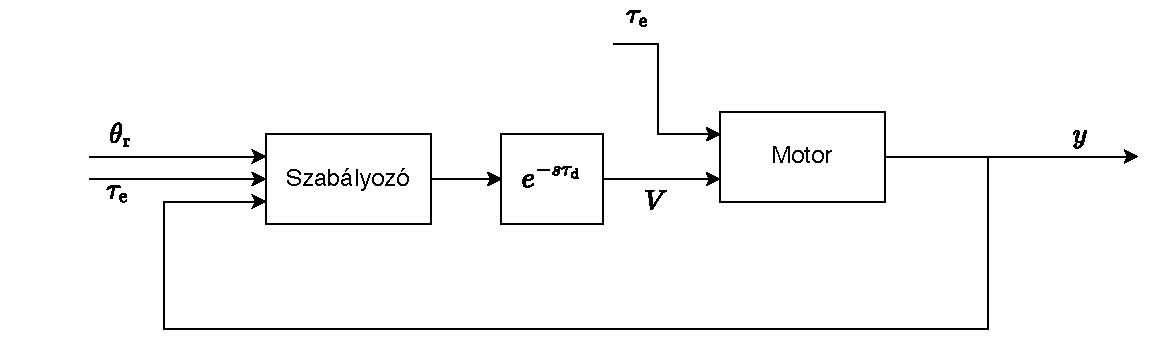
\includegraphics[width=\textwidth]{images/block_diagram_time_delay.pdf}
    \caption{Időkéséssel kiegészített egyszerűsített blokk diagram}\label{fig:block_diagram_time_delay}
    \end{center}
\end{figure}
A motor átviteli függvényei a~\eqref{eq:transfer_function} egyenletekben szerepelnek. A szabályozó dinamikáját 
az átláthatóság érdekében a következő egyenletek összegzik:
\begin{equation}
    \begin{split}
        \dot{\tilde{\BF \eta}} &= \hat{\BF A} \tilde{\BF \eta} + \hat{\BF B} y + \hat{\BF F}_\RM V V + \hat{\BF F}_\RM \tau \tau_\RM e\,, \\
        \tilde{\BF \eta} &= \tilde{\BF x}_\RM b - \BF K_\RM e y\,, \\
        V &= K_\RM r \theta_\RM r - K_\RM c \tau_\RM e - \BF K \tilde{\BF x}\,,
    \end{split}
\end{equation}
ahol a megfigyelő belső dinamikáját leíró egyenletben megjelenő mátrixok a~\eqref{eq:observer_params} kifejezésekhez hasonlóan:
\begin{align}
    \begin{split}
        \hat{\BF A} &= \BF A_\RM{bb} - \BF K_\RM e \BF A_\RM{ab}\,,\\
        \hat{\BF B} &= \hat{\BF A} \BF K_\RM e + \BF A_\RM {ba} - \BF K_\RM e A_\RM {aa}\,,\\
        \hat{\BF F} &= \BF B_\RM b - \BF K_\RM e B_\RM a\,.
    \end{split}
\end{align}
A kimeneti feszültség egyenletében található becsült állapotvektor kifejezhető a megfigyelő belső állapotával és a mért kimenettel:
\begin{equation}
    \begin{split}
        V &= K_\RM r \theta_\RM r - K_\RM c \tau_\RM e - (K_a + \BF K_\RM b \BF K_\RM e) y - \BF K_\RM b \tilde{\BF \eta}\,.
    \end{split}
\end{equation}
Behelyettesítve a megfigyelő dinamikai egyenletébe:
\begin{align}\label{eq:observer_transfer_transformed}
    \begin{split}
        \dot{\tilde{\BF \eta}} &= \hat{\BF A} \tilde{\BF \eta} + 
        \hat{\BF B} y + 
        \hat{\BF F}_\RM V\left[K_\RM r \theta_\RM r - K_\RM c \tau_\RM e - (K_a + \BF K_\RM b \BF K_\RM e) y - \BF K_\RM b \tilde{\BF \eta}\right] + 
        \hat{\BF F}_\RM \tau \tau_\RM e \\
        &= (\hat{\BF A} - \hat{\BF F}_\RM V \BF K_\RM b)\tilde{\BF \eta} + 
        [\hat{\BF B} - \hat{\BF F}_\RM V (K_\RM a + \BF K_\RM b \BF K_\RM e)]y + 
        \hat{\BF F}_\RM V K_\RM r \theta_\RM r + 
        (\hat{\BF F}_\RM \tau - \hat{\BF F}_\RM V K_\RM c) \tau_\RM e\,.
    \end{split}
\end{align}
A szabályozó dinamikája ez alapján kifejezhető egy új állapottér modell formájában:
\begin{align}\label{eq:controller_state_space}
    \begin{split}
        \dot{\tilde{\BF \eta}} &= \tilde{\BF A}\tilde{\BF \eta} + 
        \tilde{\BF B}_\RM y y + 
        \tilde{\BF B}_\RM r \theta_\RM r +
        \tilde{\BF B}_\RM \tau \tau\RM e\,, \\
        V &= \tilde{\BF C}\tilde{\BF \eta} + 
        \tilde{\BF D}_\RM y y + 
        \tilde{\BF D}_\RM r \theta_\RM r + 
        \tilde{\BF D}_\RM \tau \tau_\RM e\,,
    \end{split}
\end{align}
ahol a mátrix paraméterek~\eqref{eq:observer_transfer_transformed} szerint:
\begin{align}
    \begin{split}
        \tilde{\BF A}\ &= \hat{\BF A} - \hat{\BF F}_\RM V \BF K_\RM b\,,\\
        \tilde{\BF B}_\RM y &= \hat{\BF B} - \hat{\BF F}_\RM V (K_\RM a + \BF K_\RM b \BF K_\RM e)\,,\\
        \tilde{\BF B}_\RM r &= \hat{\BF F}_\RM V K_\RM r\,, \\
        \tilde{\BF B}_\RM \tau &= \hat{\BF F}_\RM \tau - \hat{\BF F}_\RM V K_\RM c\,, \\
        \tilde{\BF C}\ &= -\BF K_\RM b\,, \\
        \tilde{\BF D}_\RM y &= -(K_\RM a + \BF K_\RM b \BF K_\RM e)\,, \\
        \tilde{\BF D}_\RM r &= K_\RM r\,, \\
        \tilde{\BF D}_\RM \tau &= -K_\RM c\,.
    \end{split}
\end{align}
A szabályozó és a motor állapottér egyenletei időkéséssel kiegészítve a következő átviteli 
függvénnyel írhatók le:
\begin{align}
    \begin{split}
        y = \left(C^\RM V_\RM r \theta_\RM r + 
        C^\RM V_\RM \tau \tau_\RM e +
        C^\RM V_\RM y y\right)M^\RM y_\RM V e^{-s\tau_\RM d} +
        M^\RM y_\RM\tau \tau_\RM e\,,
    \end{split}
\end{align}
ahol a \(C^\RM n_\RM m\) és \(M^\RM n_\RM m\) a szabályozó és a motor átviteli függvényei adott 
bemenetekre és kimenetekre. A felső index jelöli a kimenetet, az alsó index pedig a bemenetet.
Az átviteli egyenlet zárt körben:
\begin{align}
    \begin{split}
        y = \frac{1}{1 - M^\RM y_\RM V C^\RM V_\RM y e^{-s\tau_\RM d}}
        \left[
            M^\RM y_\RM V C^\RM V_\RM r \theta_\RM r e^{-s\tau_\RM d} + 
            \left(M^\RM y_\RM\tau + M^\RM y_\RM V C^\RM V_\RM \tau e^{-s\tau_\RM d}\right) \tau_\RM e
        \right]
    \end{split}
\end{align}
alakban írható le. A motor és a szabályozó átviteli függvényei bemenettől és kimenettől 
függetlenül ugyanazokkal a pólusokkal rendelkeznek, így mindkét bemenetre ugyanazok a stabilitási 
feltételek érvényesek. Az átviteli függvény pólusait a következő egyenlet megoldásai adják:
\begin{align}\label{eq:delay_characteristic}
    \begin{split}
        &s^5 + 
        \left(c_{41} + c_{42}\frac{B_\RM e}{M_\RM e}\right)s^4 +
        \left(c_{31} + c_{32}\frac{B_\RM e}{M_\RM e} + c_{33}\frac{K_\RM e}{M_\RM e}\right)s^3 + \\
        &\left[c_{21} + c_{22}\frac{B_\RM e}{M_\RM e} + c_{23}\frac{K_\RM e}{M_\RM e} + \left(
        c_{24} + c_{25}\frac{B_\RM e}{M_\RM e} + c_{26}\frac{K_\RM e}{M_\RM e}\right)e^{-s\tau_\RM d}\right]s^2 + \\
        &\left[c_{11} + c_{12}\frac{B_\RM e}{M_\RM e} + c_{13}\frac{K_\RM e}{M_\RM e} + \left(
        c_{14} + c_{15}\frac{B_\RM e}{M_\RM e} + c_{16}\frac{K_\RM e}{M_\RM e}\right)e^{-s\tau_\RM d}\right]s + 
        c_0 \frac{K_\RM e}{M_\RM e} = 0\,.
    \end{split}
\end{align}
D-szeparációt alkalmazva az egyenlet valós és 
képzetes részei:
\begin{align}\label{eq:delay_complex_separation}
    \begin{split}
        a_4\omega^4-(a_{21} + a_{22}\cos{\omega\tau_\RM d})\omega^2+a_{12}\omega\sin{\omega\tau_\RM d} + a_0\cos{\omega\tau_\RM d} &= 0 \\
        \omega^5 -a_3\omega^3 + a_{22}\omega^2\sin{\omega\tau_\RM d} + (a_{11} + a_{12}\cos{\omega\tau_\RM d})\omega - a_0\sin{\omega\tau_\RM d}  &= 0 \,,
    \end{split}
\end{align}
melyek \(s=jw\) behelyettesítés után adódnak. Az új együtthatók~\eqref{eq:delay_characteristic} alapján:
\begin{align}
    \begin{split}
        a_4 &= c_{41} + c_{42}\frac{B_\RM e}{M_\RM e}\\ 
        a_3 &= c_{31} + c_{32}\frac{B_\RM e}{M_\RM e} + c_{33}\frac{K_\RM e}{M_\RM e}\\ 
        a_{21} &= c_{21} + c_{22}\frac{B_\RM e}{M_\RM e} + c_{23}\frac{K_\RM e}{M_\RM e}\\ 
        a_{22} &= c_{24} + c_{25}\frac{B_\RM e}{M_\RM e} + c_{26}\frac{K_\RM e}{M_\RM e}\\ 
        a_{11} &= c_{11} + c_{12}\frac{B_\RM e}{M_\RM e} + c_{13}\frac{K_\RM e}{M_\RM e}\\ 
        a_{12} &= c_{14} + c_{15}\frac{B_\RM e}{M_\RM e} + c_{16}\frac{K_\RM e}{M_\RM e}\\ 
        a_0 &= c_0 \frac{K_\RM e}{M_\RM e}\,.
    \end{split}
\end{align}
A~\eqref{eq:delay_complex_separation}-ben szereplő egyenletrendszert megoldva \(\frac{B_\RM e}{M_\RM e}\)
és \(\frac{K_\RM e}{M_\RM e}\) kifejezésekre egy paraméteres görbe adódik. 
A független paraméter \(\omega\) a stabilitás határán fellépő csillapítatlan rezgés frekvenciájával
arányos. A görbe minden pontjához egy tisztán képzetes póluspár vagy nulla kapcsolódik. 
A nulla megoldások a \(\frac{K_\RM e}{M_\RM e} = 0\) egyenesen helyezkednek el. 
A kapott görbét a~\ref{tab:delay_stab_params}. táblázat paramétereit behelyettesítve 
a~\ref{fig:time_delay_stab_map}. ábra mutatja. A kontúrvonalakon szereplő értékek \(\tau_\RM d\)
időkésés különböző értékeit jelölik szekundumban kifejezve.

\begin{table}[ht]
    \small\centering
    \caption{A folytonos idejű stabilitásvizsgálatnál alkalmazott paraméterek}\label{tab:delay_stab_params}
    \tabcolsep=1pt
    \begin{tabular}{l>{~}l>{\quad}rl}
        \toprule
        \multicolumn{2}{c}{Szimbólum és paraméter név} & \multicolumn{2}{c}{Érték} \\ \midrule
        \(J\) & Motor tehetetlensége & 0.01 & \(\RM{kg\cdot m^2}\) \\
        \(K_\RM m\) & Motor nyomatékállandója & 0.01 & \(\RM{Nm\cdot A^{-1}}\) \\
        \(B_\RM m\) & Motormodell viszkózus csillapítása & 0.1 & \(\RM{kg\cdot m^2\cdot s^{-1}}\) \\
        \(L\) & Motor induktivitása & 0.2 & H \\
        \(R\) & Motor ellenállása & 1 & \(\Omega\) \\
        \(p\) & További pólusok & -15 & \(\RM{rad \cdot s^{-1}}\) \\
        \(K_\RM c\) & Nyomaték kompenzációs együttható & -50 & \(\RM{V \cdot N^{-1} m^{-1}}\) \\
        \bottomrule
    \end{tabular}
\end{table}

\begin{figure}[H]
    \begin{center}
    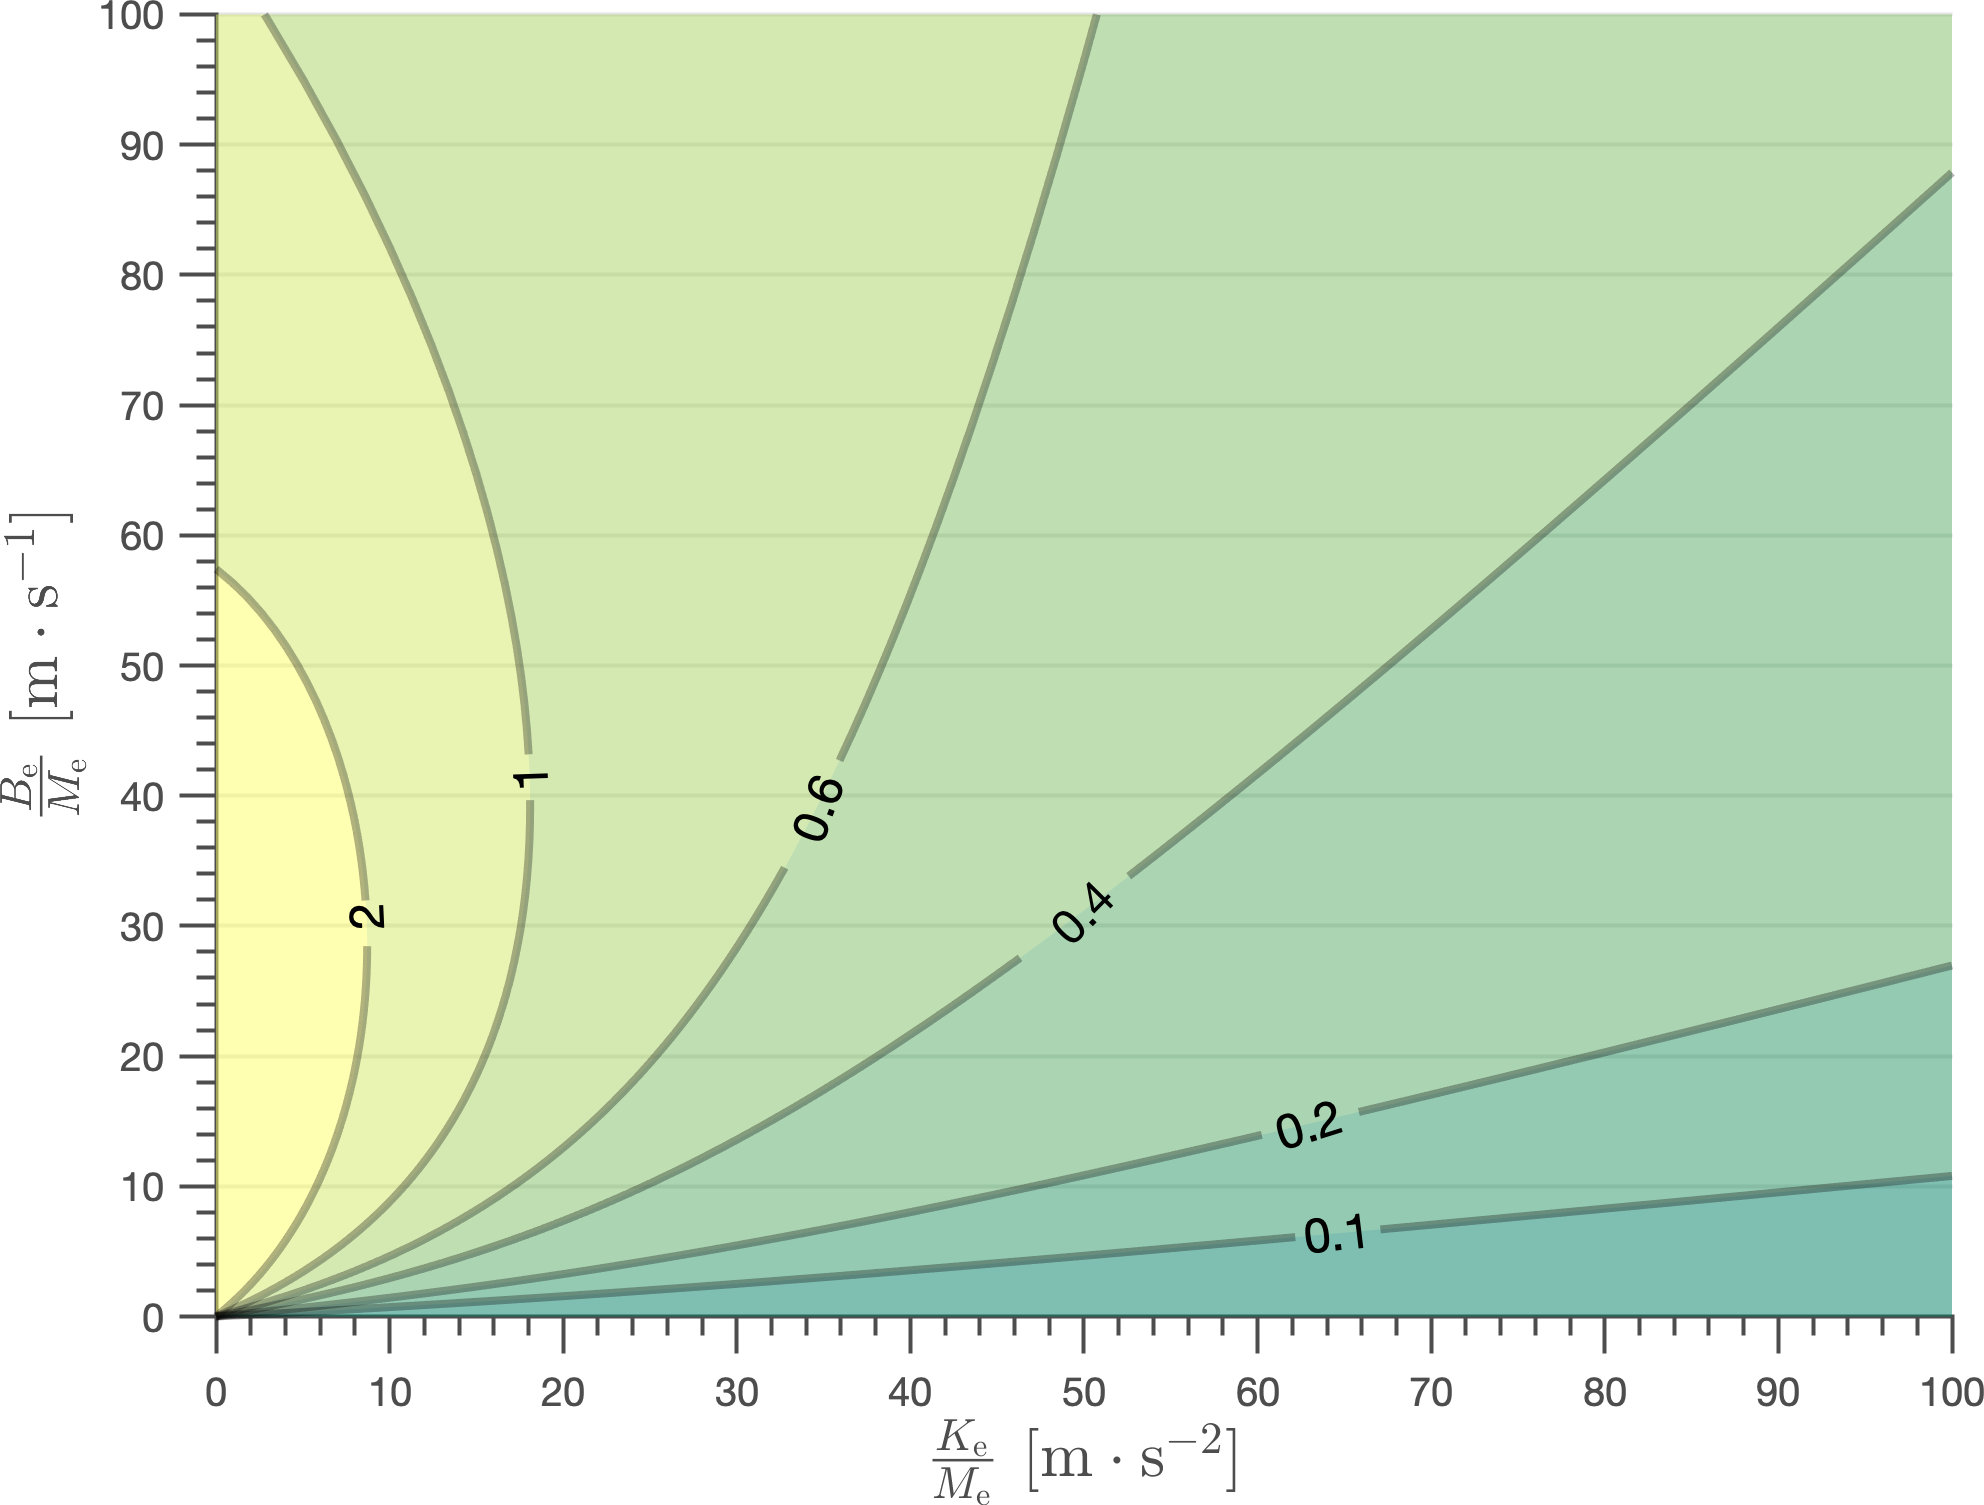
\includegraphics[width=\textwidth]{images/time_delay_stab_map.png}
    \caption{Folytonos idejű stabilitástérkép}\label{fig:time_delay_stab_map}
    \end{center}
\end{figure}

Időkésés nélkül a görbe pontjai a \(\frac{B_\RM e}{M_\RM e} = 0\) egyenesen maradnak.
A behatárolt stabilitástartomány éppen megegyezik a Routh--Hurwitz kritérium által 
kapott tartománnyal, tehát:
\begin{equation}
    M_\RM e > 0,~~B_\RM e > 0,~~K_\RM e > 0.
\end{equation}
Az időkésés növekedésével egyre szűkül a stabil tartomány, egy kritikus érték alatt azonban
csak \(\frac{K_\RM e}{M_\RM e}\) kifejezésre adódik maximum, \(\frac{B_\RM e}{M_\RM e}\)
tetszőleges pozitív értéket felvehet. A kritikus időkésés felett egy véges területet határolnak be 
a görbe \(\omega > 0\) és \(\omega = 0\) szegmensei. 

\section{Stabilitás diszkrét időben}
A folytonos időben végzett stabilitásvizsgálat alapján belátható, hogy az 
időkésés korlátozza az impedanciamodell által előírható paramétereket.
A valós rendszerben egy digitális feldolgozóegység végzi el a szabályozó jel
meghatározásához szükséges számításokat, közel azonos időnként. Két ilyen 
ciklus között a szabályozó jel állandó marad. Ezeket figyelembe véve a 
folytonos időben végzett stabilitásvizsgálat eredménye tovább pontosítható.
\begin{figure}[ht]
    \begin{center}
    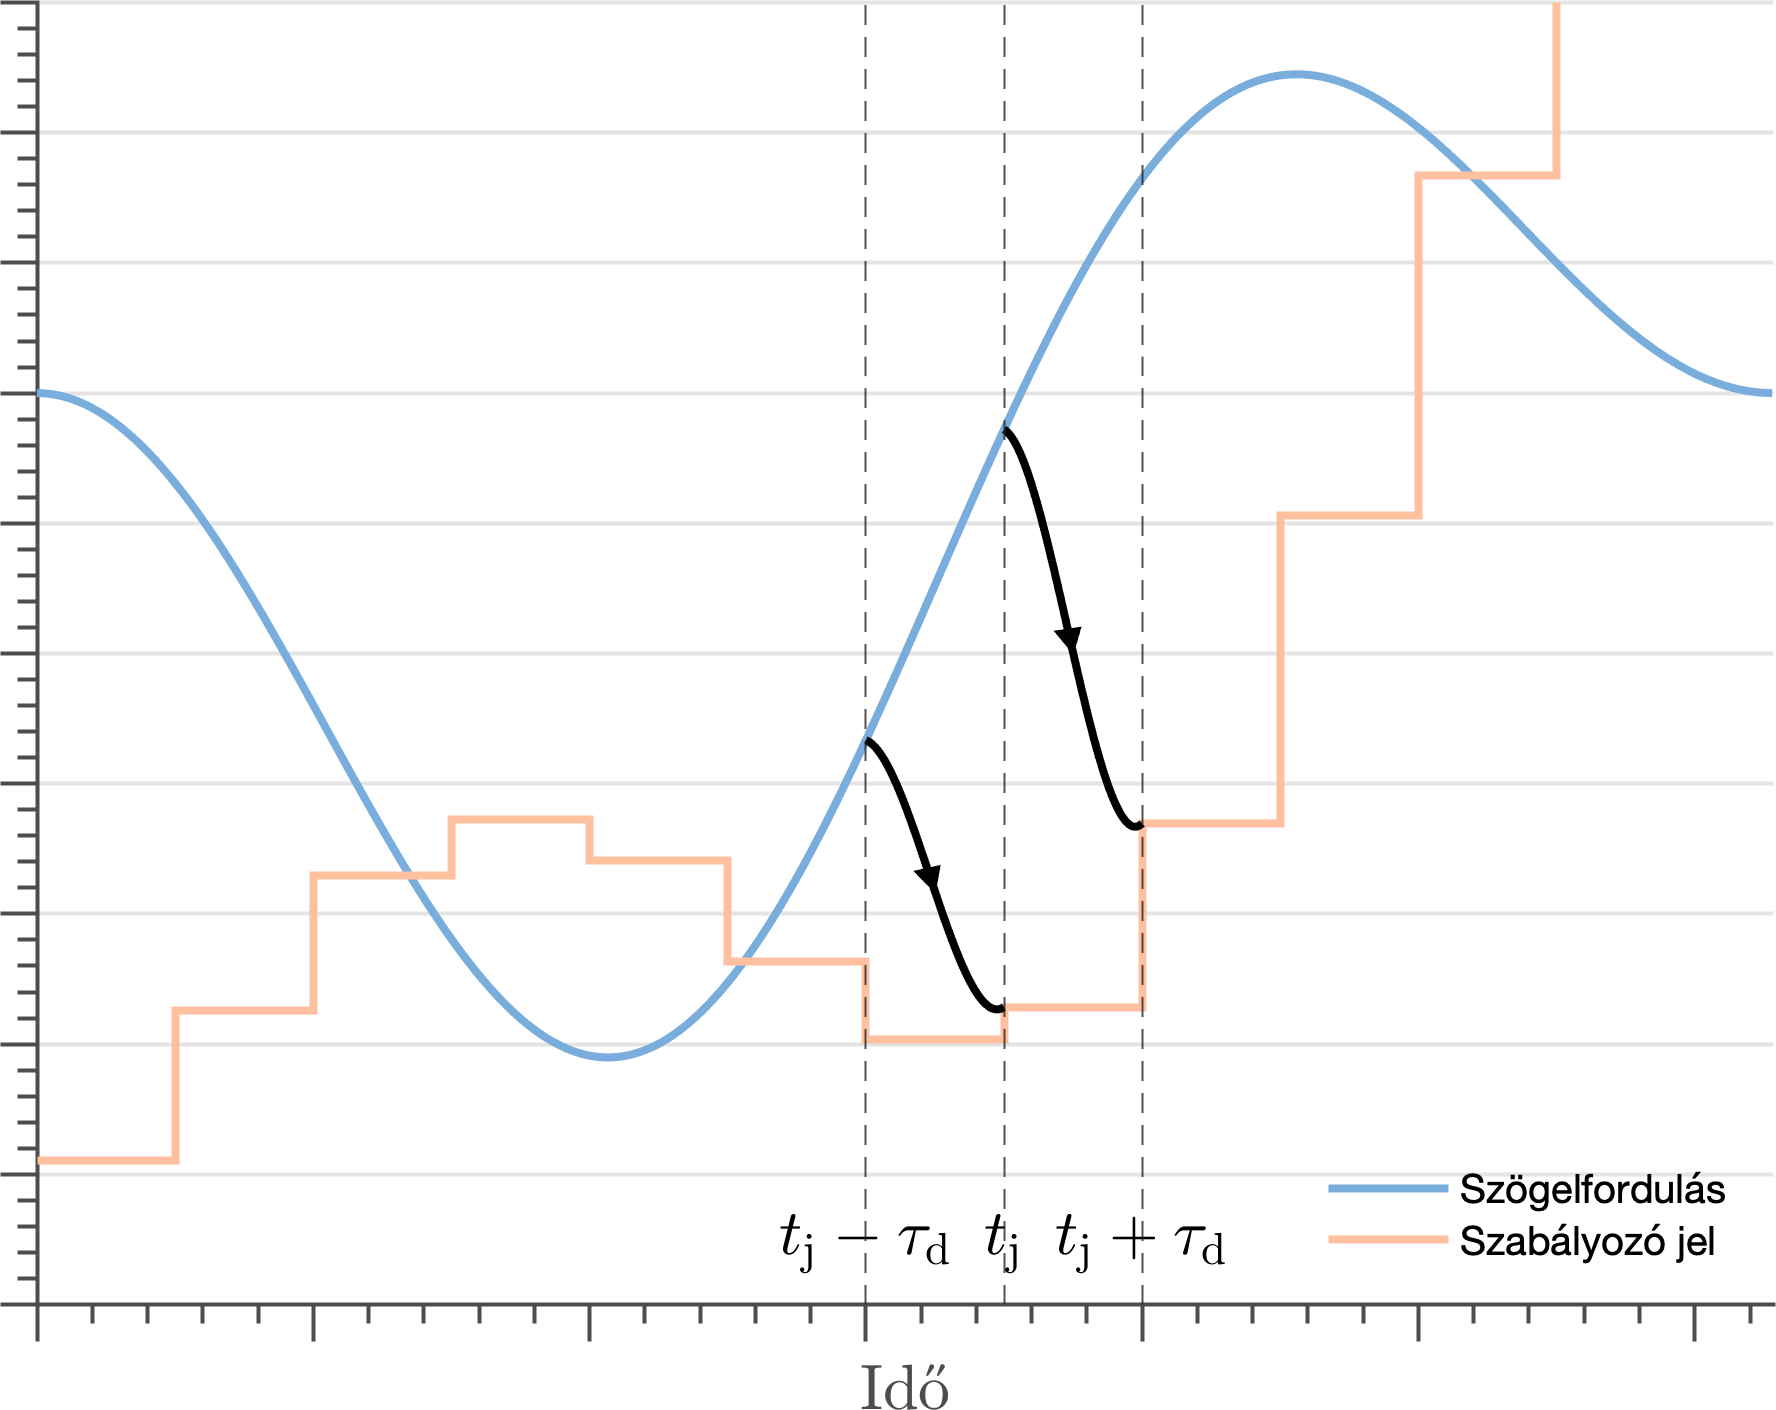
\includegraphics[width=12cm]{images/time_delay_example_discrete.png}
    \caption{Reprezentatív ábra az időkésés hatásáról diszkrét időben}\label{fig:time_delay_example_discrete}
    \end{center}
\end{figure}

A mért szögelfordulás és a diszkrét idejű szabályozó jel kapcsolatát szemlélteti a~\ref{fig:time_delay_example_discrete}. ábra.
Két mintavételezési pont között a szabályozó jel változatlan marad (zero-order hold). A mért szögelfordulás érték 
feldolgozása után az új szabályozó jel mindig egy mintavételezési periódussal később jelenik meg a motor bemenetén.
A továbbiakban feltételezett, hogy a jelfeldolgozáshoz szükséges időn kívül minden egyéb késés elhanyagolható, 
így a mintavételezési periódus megegyezik a korábban bevezetett \(\tau_\RM d\) időkéséssel. Legyen \(C(t-\tau(t))\) 
a szabályozó jel időfüggvénye. Ebben az alakban a mintavételezési pontok között akkor marad állandó a kimenet, ha 
az időkésés maga (\(\tau(t)\)) egy periodikus fűrész jelet követ, ahogy a~\ref{fig:time_delay_example_zoh}. ábra is mutatja.
\begin{figure}[H]
    \begin{center}
    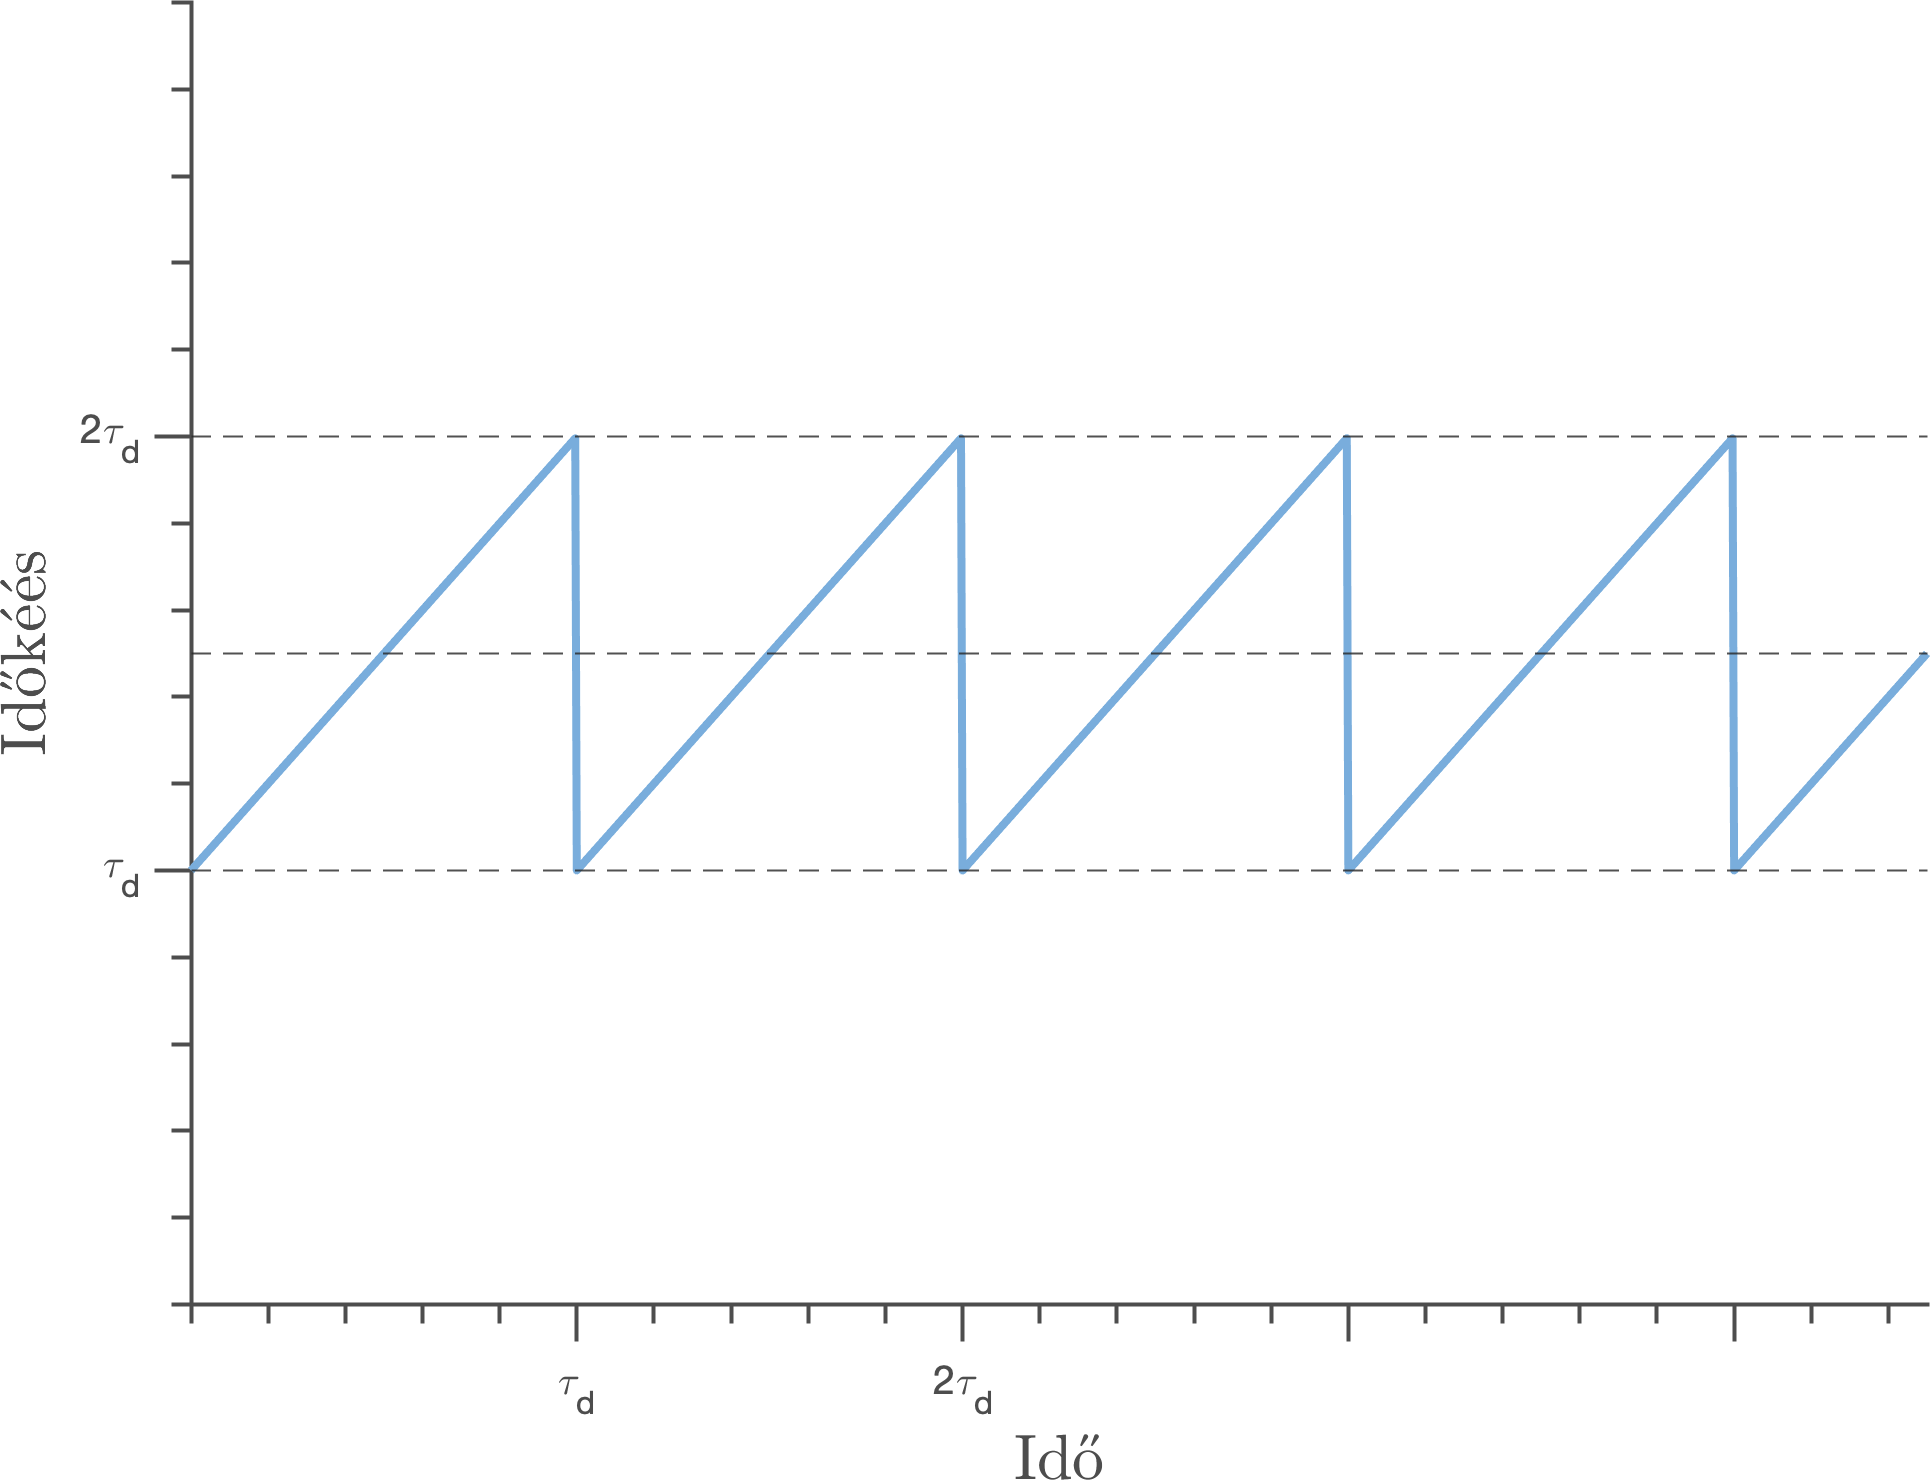
\includegraphics[width=12cm]{images/delay_zoh_example_discrete.png}
    \caption{Az időkésés periodikus függvénye}\label{fig:time_delay_example_zoh}
    \end{center}
\end{figure}

A diszkrét idejű stabilitásvizsgálathoz először diszkretizálni kell a szabályozó folytonos idejű állapottér modelljét.
Ehhez legyen a kiindulási alap a~\eqref{eq:controller_state_space} egyenletek által definiált modell.
Beszorozva mindkét oldalt \(e^{-\tilde {\BF A} t}\)-vel:
\begin{align}
    \begin{split}
        e^{-\tilde {\BF A} t}\dot{\tilde{\BF \eta}}(t) &= e^{-\tilde {\BF A} t}\tilde {\BF A} \tilde{\BF \eta}(t) +
        e^{-\tilde {\BF A} t}\left[\tilde{\BF B}_\RM y y(t) + 
        \tilde{\BF B}_\RM r \theta_\RM r(t) +
        \tilde{\BF B}_\RM \tau \tau_\RM e(t)\right] \\
        \frac{\RM d}{\RM d t}\left(e^{-\tilde {\BF A} t}\tilde{\BF \eta}(t)\right) &= e^{-\tilde {\BF A} t}\left[\tilde{\BF B}_\RM y y(t) + 
        \tilde{\BF B}_\RM r \theta_\RM r(t) +
        \tilde{\BF B}_\RM \tau \tau_\RM e(t)\right]\,, 
    \end{split}        
\end{align}
a kapott egyenletet integrálva:
\begin{align}\label{eq:controller_state_integral}
    \begin{split}
        e^{-\tilde {\BF A} t}\tilde{\BF \eta}(t) - e^0 \tilde{\BF \eta}(0) &= \int_{0}^{t} e^{-\tilde {\BF A} t'}\left[\tilde{\BF B}_\RM y y(t') + 
        \tilde{\BF B}_\RM r \theta_\RM r(t') +
        \tilde{\BF B}_\RM \tau \tau_\RM e(t')\right] \RM dt' \\
        \tilde{\BF \eta}(t) &= e^{\tilde {\BF A} t}\tilde{\BF \eta}(0) + \int_{0}^{t} e^{\tilde {\BF A} (t-t')}\left[\tilde{\BF B}_\RM y y(t') + 
        \tilde{\BF B}_\RM r \theta_\RM r(t') +
        \tilde{\BF B}_\RM \tau \tau_\RM e(\tau)\right] \RM dt'\,.
    \end{split}        
\end{align}
A mintavételezési periódus alatt a szabályozó összes bemenete konstans marad, így a bemenetek az 
integrálon kívülre helyezhetők. Legyen \(\tilde{\BF \eta}[k] \stackrel{\text{def}}{=} \tilde{\BF \eta}(k\tau_\RM d)\) a 
a szabályázó belső állapota a \(k\)-adik diszkrét időlépésnél. Ezzel a~\eqref{eq:controller_state_integral}. 
egyenlet a \(k\)-adik és a (\(k+1\))-edik lépéseknél:
\begin{align}
    \begin{split}
        \tilde{\BF \eta}[k] &= e^{\tilde {\BF A} k\tau_\RM d}\tilde{\BF \eta}(0) + \int_{0}^{k\tau_\RM d} e^{\tilde {\BF A} (k\tau_\RM d-t')}\left[\tilde{\BF B}_\RM y y(t') + 
        \tilde{\BF B}_\RM r \theta_\RM r(t') +
        \tilde{\BF B}_\RM \tau \tau_\RM e(t')\right]\RM dt' \\
        \tilde{\BF \eta}[k+1] &= e^{\tilde {\BF A}\tau_\RM d}\tilde{\BF \eta}[k] + \int_{k\tau_\RM d}^{(k+1)\tau_\RM d} e^{\tilde {\BF A} (k\tau_\RM d + \tau_\RM d-t')}\left[\tilde{\BF B}_\RM y y(t') + 
        \tilde{\BF B}_\RM r \theta_\RM r(t') +
        \tilde{\BF B}_\RM \tau \tau_\RM e(t')\right] \RM dt' \\
        \tilde{\BF \eta}[k+1] &= e^{\tilde {\BF A}\tau_\RM d}\tilde{\BF \eta}[k] + \int_{k\tau_\RM d}^{(k+1)\tau_\RM d} e^{\tilde {\BF A} (k\tau_\RM d + \tau_\RM d-t')}\RM dt'\left[\tilde{\BF B}_\RM y y[k] + 
        \tilde{\BF B}_\RM r \theta_\RM r[k] +
        \tilde{\BF B}_\RM \tau \tau_\RM e[k]\right] \\
        \tilde{\BF \eta}[k+1] &= e^{\tilde {\BF A}\tau_\RM d}\tilde{\BF \eta}[k] + \tilde{\BF A}^{-1}\left(e^{\tilde {\BF A}\tau_\RM d}-\BF I\right)\left[\tilde{\BF B}_\RM y y[k] + 
        \tilde{\BF B}_\RM r \theta_\RM r[k] +
        \tilde{\BF B}_\RM \tau \tau_\RM e[k]\right]\,.
    \end{split}        
\end{align}
Tehát a diszkrét idejű szabályozó állapotér modelljét leírő mátrixok:
\begin{align}\label{eq:discrete_controller_matrices}
    \begin{split}
        \tilde{\BF A}_\RM d &= e^{\tilde {\BF A}\tau_\RM d} \\
        \tilde{\BF B}_\RM d &= \tilde{\BF A}^{-1}\left(e^{\tilde {\BF A}\tau_\RM d}-\BF I\right)\left[\tilde{\BF B}_\RM y~~\tilde{\BF B}_\RM r~~\tilde{\BF B}_\RM \tau\right] \\
        \tilde{\BF C}_\RM d &= \tilde{\BF C} \\
        \tilde{\BF D}_\RM d &= \tilde{\BF D} \,,
    \end{split}        
\end{align}
ahol a mátrix exponenciális kifejezés szükség esetén például Taylor-polinommal közelíthető. A további számítások ezt 
a pontos alakot használják.

Következő lépésként a zárt kör dinamkáját is ki kell fejezni a diszkrét időlépések függvényeként. 
A szabályozónál alkalmazott levezetéshez hasonlóan~\eqref{eq:state_space}-ban szereplő mátrixok alapján:
\begin{align}\label{eq:discrete_motor_state}
    \begin{split}    
        \BF x[k+1] &= e^{\BF A \tau_\RM d}\BF x[k] + 
        \BF A^{-1}\left(e^{\BF A \tau_\RM d} - \BF I\right)\BF B_\RM V V[k-1] + 
        \int_{k\tau_\RM d}^{(k+1)\tau_\RM d} e^{\BF A (k\tau_\RM d + \tau_\RM d-t')}\BF B_\RM \tau \tau_\RM e(t')~\RM dt'\\
        y[k] &= \BF C \BF x[k]\,.
    \end{split}        
\end{align}
ahol megjelenik \(V[k-1]\) a szabályozó jel egy egész mintavételezési periódussal késleltetett értéke. 
Legyenek a diszkretizált motormodell új paraméterei:
\begin{align}\label{eq:discrete_motor_matrices}
    \begin{split}
        \BF A_\RM d &= e^{\BF A\tau_\RM d} \\
        \BF B_\RM d &= \BF A^{-1}\left(e^{\BF A\tau_\RM d}-\BF I\right)\BF B_\RM V \\
        \BF C_\RM d &= \BF C \\
        \BF D_\RM d &= \BF D \,.
    \end{split}        
\end{align}

A stabilitásvizsgálathoz a bemenet zérus. A következőkben a zárt kör teljes dinamikájának levezetése 
következik zérus bemenettel. A~\eqref{eq:discrete_motor_state} állapotegyenletbe behelyettesítve a 
szabályozó késleltetett kimenetét:
\begin{align}
    \begin{split}
    \BF x[k+1] &= \BF A_\RM d x[k] + 
    \BF B_\RM d \left(\tilde{\BF C}_\RM d \tilde{\BF \eta}[k-1] + 
    \tilde{\BF D}_\RM {d,y} y[k-1]\right)\,,
    \end{split}        
\end{align}
Felhasználva \(\tilde{\BF \eta}\) és a paraméterek definícióját:
\begin{align}\label{eq:discrete_motor_state_closed}
    \begin{split}
        \BF x[k+1] &= \BF A_\RM d x[k] - 
        \BF B_\RM d \BF K_\RM a y[k-1] - 
        \BF B_\RM d \BF K_\RM b \tilde{\BF x}_\RM b[k-1] \\
        &= \BF A_\RM d x[k] - 
        \BF B_\RM d \BF K \BF x[k-1] +
        \BF B_\RM d \BF K_\RM b \BF e[k-1]\,.
    \end{split}        
\end{align}
A becsült állapot hibájának differencia egyenletei pedig:
\begin{align}
    \begin{split}
        \BF e[k+1] &= \BF x_\RM b[k+1] - \tilde{\BF x}_\RM b[k+1] \\
        &= \BF E_{\RM{xa},k}\BF x_\RM a[k] + 
        \BF E_{\RM{xb},k}\BF x_\RM b[k] + 
        \BF E_{\RM x,k-1}\BF x[k-1] + 
        \BF E_{\RM e,k}\BF e[k] + 
        \BF E_{\RM e,k-1}\BF e[k-1]
        \,,
    \end{split}        
\end{align}
ahol a mátrix együtthatók:
\begin{align}
    \begin{split}
        \BF E_{\RM{xa},k} &= \BF A_\RM{d,ba} + 
        \tilde{\BF A}_\RM d \BF K_\RM e -
        \BF K_\RM e \BF A_\RM{d,aa} \\
        \BF E_{\RM{xb},k} &= \BF A_\RM{d,bb} + 
        \tilde{\BF A}_\RM d -
        \BF K_\RM e \BF A_\RM{d,ab} \\
        \BF E_{\RM x,k-1} &= -(\BF B_\RM{d,b} -
        \BF K_\RM e \BF B_\RM{d,a})\RM K \\
        \BF E_{\RM e,k} &= \tilde{\BF A}_\RM d \\
        \BF E_{\RM e,k-1} &= (\BF B_\RM{d,b} -
        \BF K_\RM e \BF B_\RM{d,a})\RM K_\RM b\,.
    \end{split}        
\end{align}
A~\eqref{eq:pos_control_dynamics} egyenlethez hasonlóan a 
teljes rendszer belső állapotának dinamikája:
\begin{align}
    \begin{split}
        \begin{bmatrix}
        \BF x[k] \\
        \BF e[k] \\
        \BF x[k+1] \\ 
        \BF e[k+1] \\ 
        \end{bmatrix} &=
        \begin{bmatrix}
            \BF 0 & \BF 0 & \BF I & \BF 0 \\
            \BF 0 & \BF 0 & \BF 0 & \BF I \\
            -\BF B_\RM d \BF K & \BF B_\RM d \BF K_\RM b & \BF A_\RM d & \BF 0 \\
            \BF E_{\RM x,k-1} & \BF E_{\RM e,k-1} & \BF E_{\RM x,k} & \BF E_{\RM e,k} \\ 
        \end{bmatrix}
        \begin{bmatrix}
            \BF x[k-1] \\
            \BF e[k-1] \\
            \BF x[k] \\ 
            \BF e[k] \\ 
        \end{bmatrix}\,.
    \end{split}        
\end{align}
A stabilitás feltétele, hogy a kapott diszkrét állapot átmeneti mátrix minden sajátértéke abszolút 
értékben egynél szigorúan kisebb legyen. A~\ref{fig:time_delay_stab_map_discrete}. ábra a~\ref{tab:delay_stab_params_discrete}. táblázat paraméterei alapján numerikusan 
meghatározott stabilitástérképet ábrázolja \(K_\RM e\) és \(B_\RM e\) impedancia paraméterek függvényében. 
\begin{table}[H]
    \small\centering
    \caption{A diszkrét idejű stabilitásvizsgálatnál alkalmazott paraméterek}\label{tab:delay_stab_params_discrete}
    \tabcolsep=1pt
    \begin{tabular}{l>{~}l>{\quad}rl}
        \toprule
        \multicolumn{2}{c}{Szimbólum és paraméter név} & \multicolumn{2}{c}{Érték} \\ \midrule
        \(J\) & Motor tehetetlensége & 0.01 & \(\RM{kg\cdot m^2}\) \\
        \(K_\RM m\) & Motor nyomatékállandója & 0.01 & \(\RM{Nm\cdot A^{-1}}\) \\
        \(B_\RM m\) & Motormodell viszkózus csillapítása & 0.1 & \(\RM{kg\cdot m^2\cdot s^{-1}}\) \\
        \(L\) & Motor induktivitása & 0.2 & H \\
        \(R\) & Motor ellenállása & 1 & \(\Omega\) \\
        \(p\) & További pólusok & -15 & \(\RM{rad \cdot s^{-1}}\) \\
        \(M_\RM e\) & Előírt tehetetlenség & 0.015 & \(\RM{kg\cdot m^2}\) \\
        \(\tau_\RM d\) & Mintavételezśi idő & 0.1 & \(\RM{s}\) \\
        \bottomrule
    \end{tabular}
\end{table}
A sajátértékek egy 150x150 méretű, egyenletesen elosztott rács pontjain lettek meghatározva. Ezután 
az előbb említett stabilitási feltétel szerint különítettem el a stabil pontokat. Majd a 
stabil pontok Delaunay-háromszögelése~\citep{Okabe00} és annak konvex burka került kirajzolásra.
\begin{figure}[H]
    \begin{center}
    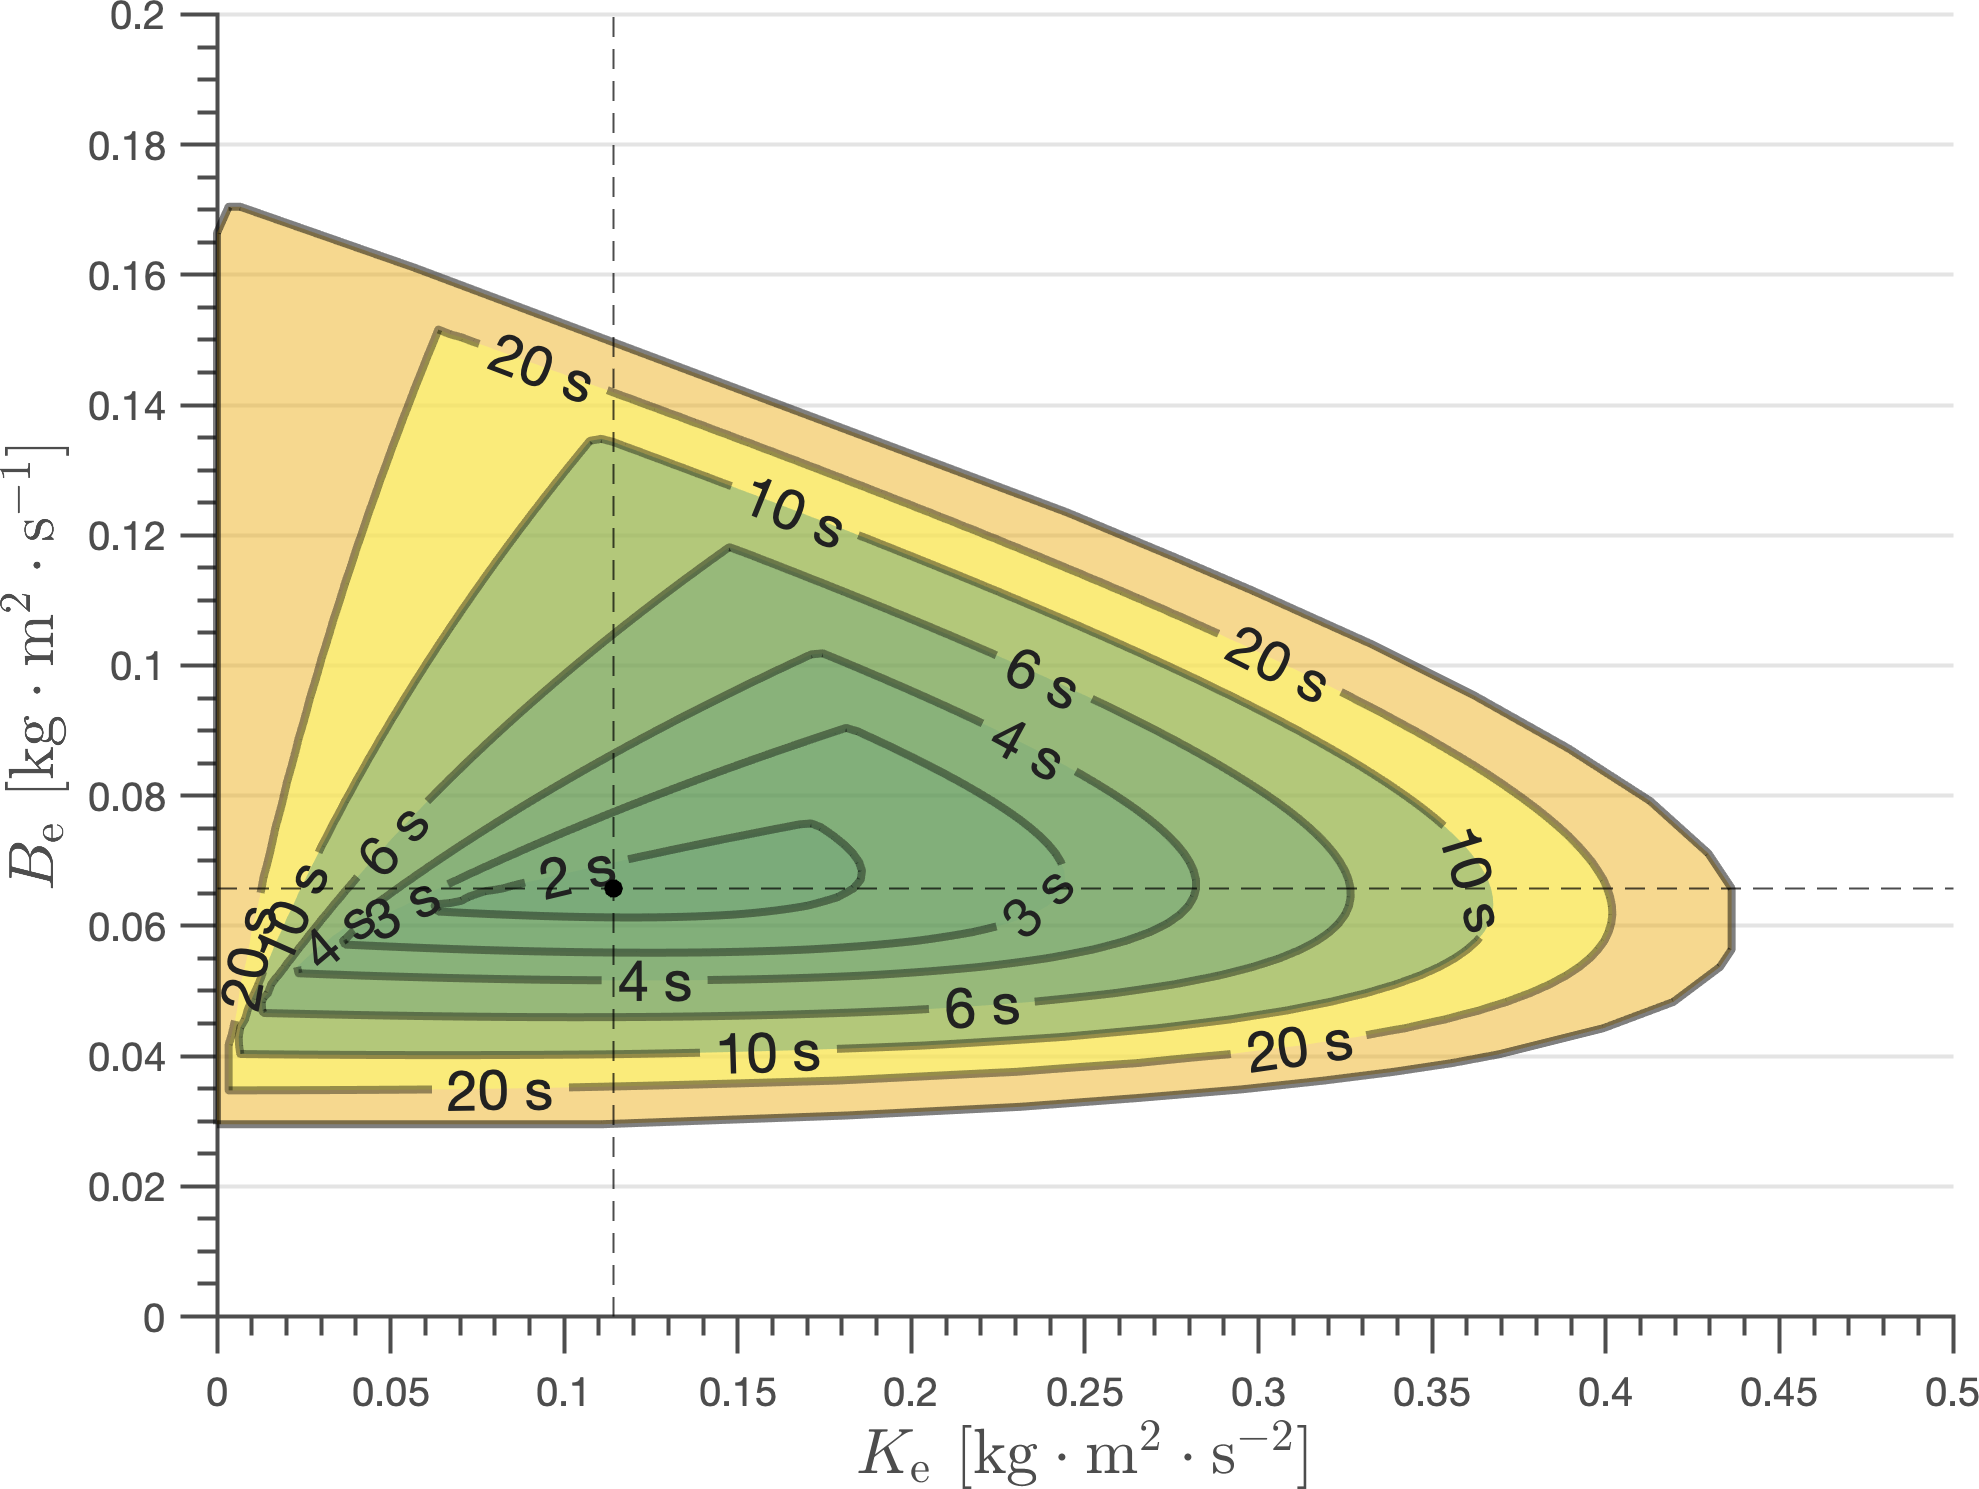
\includegraphics[width=\textwidth]{images/time_delay_stab_map_discrete.png}
    \caption{Diszkrét idejű stabilitástérkép}\label{fig:time_delay_stab_map_discrete}
    \end{center}
\end{figure}
A kontúrok a különböző becsült beállási időket jelölnek, melyek a legnagyobb abszolút értékű sajátérték 
alapján lettek meghatározva 2\%-os hibasávot alapul véve:
\begin{align}
    \begin{split}
        t_\RM s \approx \tau_\RM d \frac{\ln{0.02}}{\ln{|\lambda|_\RM{max}}}\,,
    \end{split}        
\end{align}
ahol \(\tau_\RM d\) a mintavételezési idő és \(|\lambda|_\RM{max}\) jelöli a legnagyobb sajátértéket 
abszolút értékben. Az alkalmazott paraméterekkel a minimális beállási idő közelítőleg 1.2 s. 

A diszkretizáció negatív hatással van a rendszer stabilitására. A folytonos idejű időkéséses rendszernél 0.1 s 
időkéséssel még mindig végtelen nagy a stabil régió ugyanezen paraméterekkel. Az impedanciamodell által 
előírt beállási időt összehasonlítva a becsült beállási idővel ábrázolja a~\ref{fig:time_delay_stab_map_discrete_diff}.
ábra.

\begin{figure}[H]
    \begin{center}
    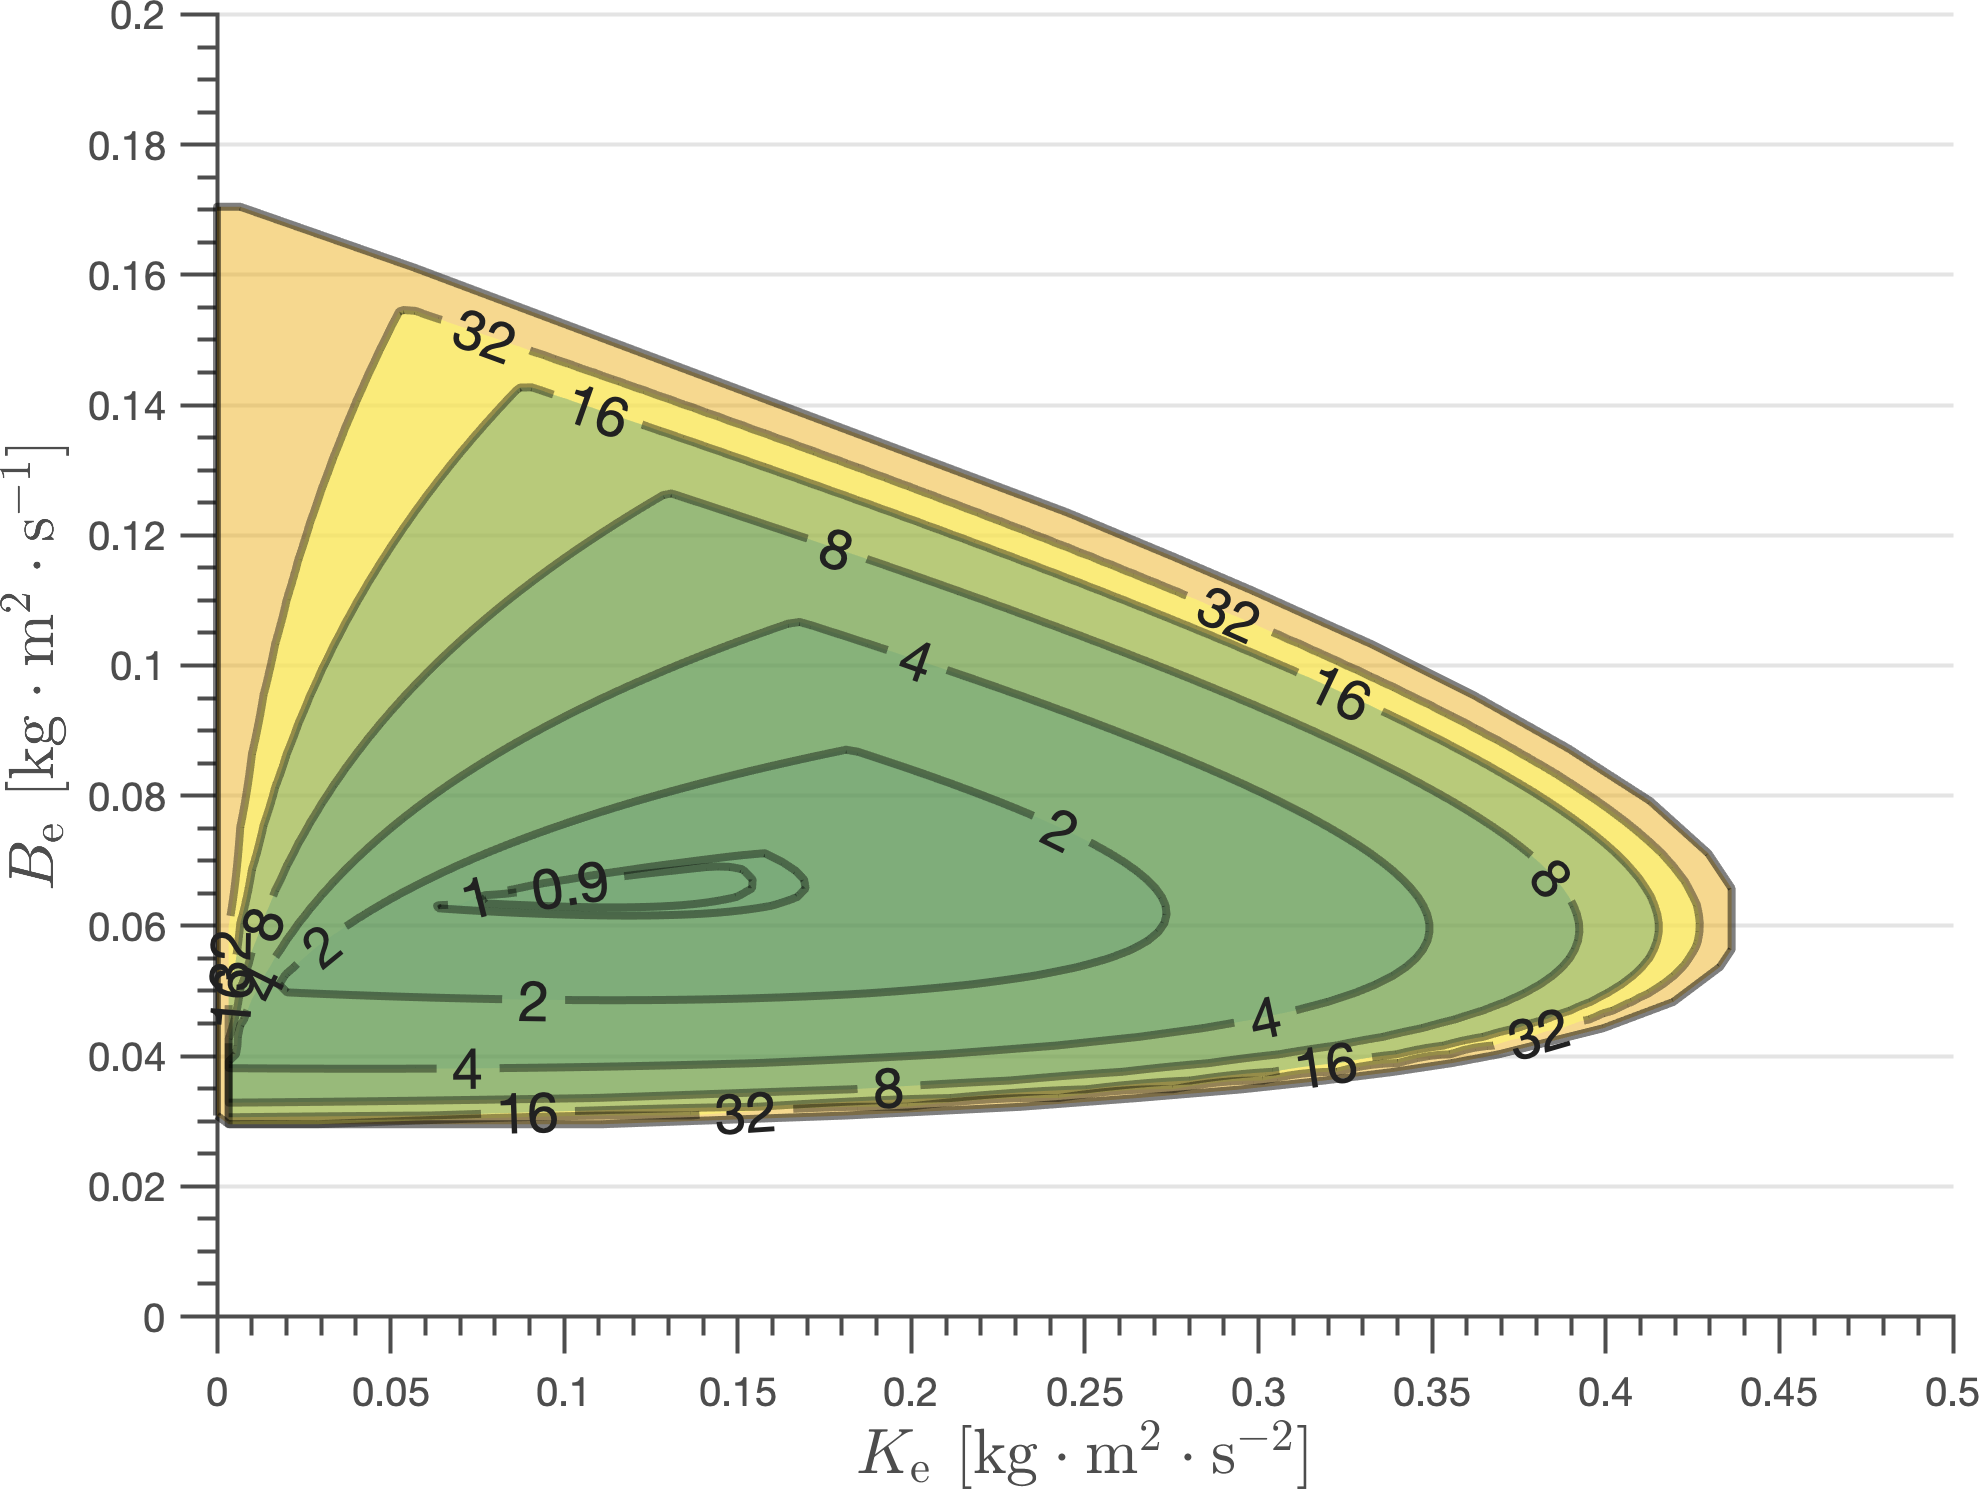
\includegraphics[width=\textwidth]{images/time_delay_stab_map_discrete_diff.png}
    \caption{Diszkrét idejű stabilitástérkép}\label{fig:time_delay_stab_map_discrete_diff}
    \end{center}
\end{figure}

A kontúrok a becsült és az előírt beállási idők hányadosát jelölik. Az alkalmazás specifikációjától függően lehet, 
hogy csak egy igen kis része felhasználható a stabil tartomáynak. Az ábrán megfigyelhető, hogy van olyan tartomány is, 
ahol az előírtnál gyorsabban áll be a rendszer.

A stabilitási határon legalább egy sajátérték vagy komplex konjugált pár abszolút értékben egy. Ennek következtében a rendszer 
\(t\rightarrow\infty\) határértékben csillapítatlan rezgőmozgást végez. A rezgőmozgás frekvenciája és az 
impedanciamodell paraméterei közötti összefüggés numerikusan meghatározható például a diszkrét 
Fourier-transzformáció segítségével. A legnagyobb frekvencia a mintavételezési frekvencia fele a Nyquist--Shannon 
mintavételezési tétel alapján 
\begin{align}
    f_\RM{max} = \frac{1}{2\tau_\RM d}\,.
\end{align}

A frekvencia felbontás pedig a mintavételek száma és a mintavételezési frekvencia alapján
\begin{align}
    \Delta f = \frac{1}{N\tau_\RM d}\,.
\end{align}

A stabil tartomány jobb széle \(B_\RM e\) értékével lett paraméterezve. Ezután minden pontban  
\(N = 100\) időlépésen át lett szimulálva a rendszer. A diszkrét Fourier-transzformált 
legnagyobb abszolút értékű frekvenciája és \(B_\RM e\) közötti kapcsolat látható 
a~\ref{fig:time_delay_stab_map_discrete_fourier}. ábra jobb oldali grafikonján. A vízszintes 
tengelyre a csillapítatlan rezgési frenvencia és a mintavételezési frekvencia hányadosa került.
\begin{figure}[H]
    \begin{center}
    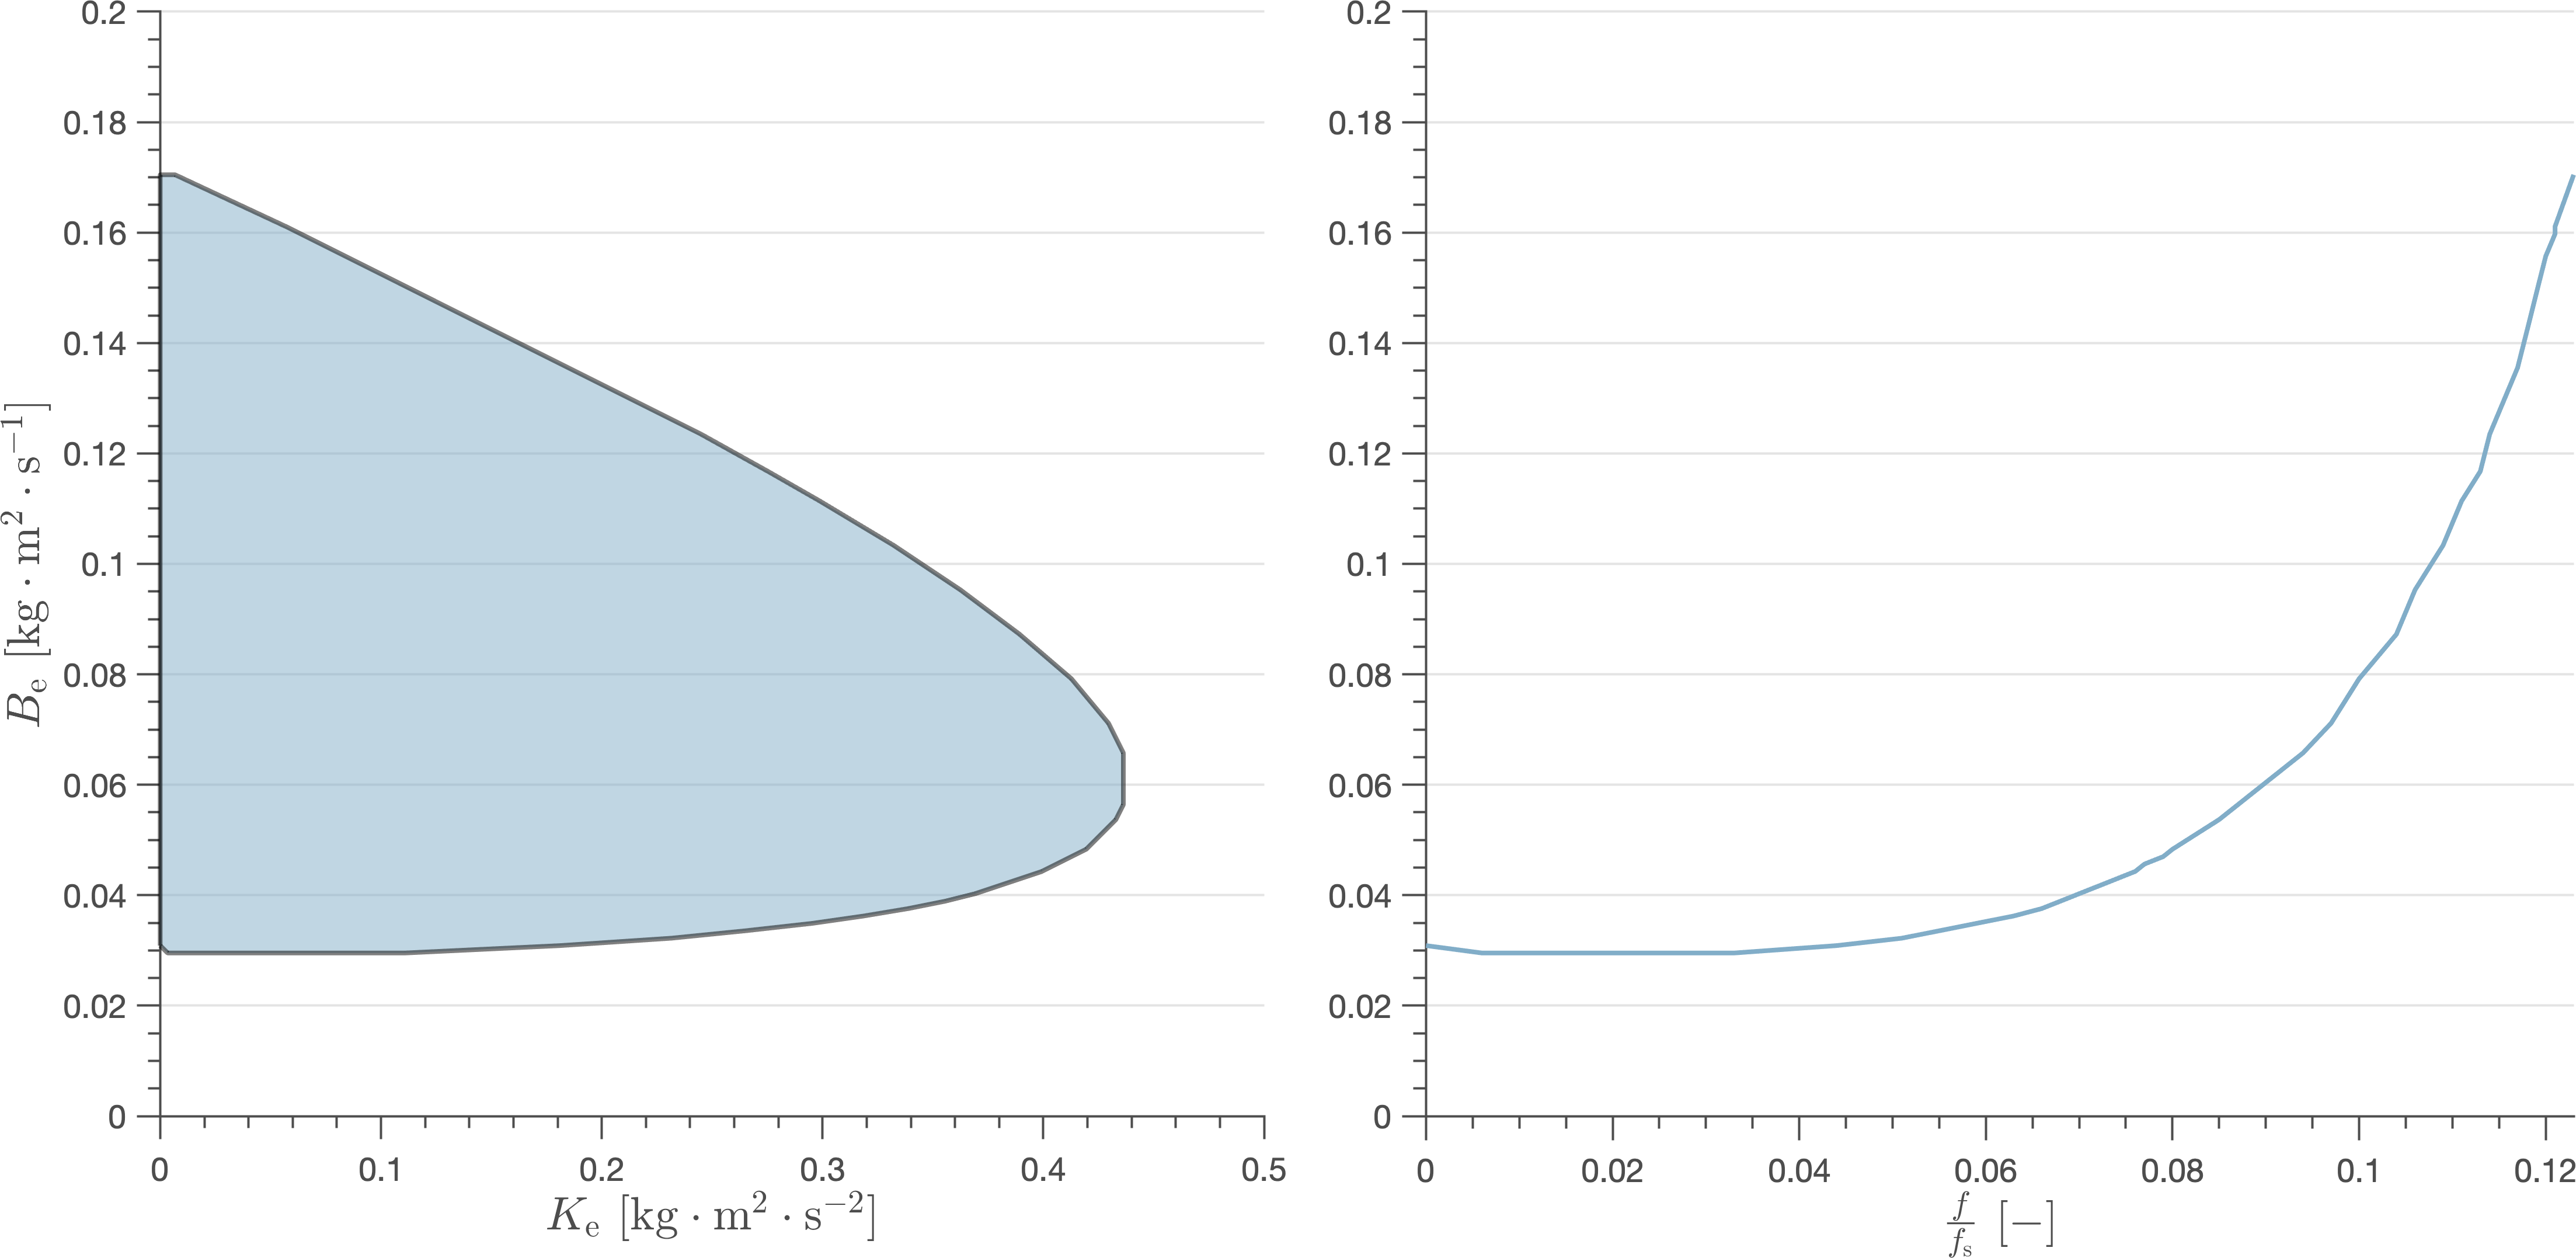
\includegraphics[width=\textwidth]{images/time_delay_stab_map_discrete_fourier.png}
    \caption{Diszkrét idejű stabilitástérkép}\label{fig:time_delay_stab_map_discrete_fourier}
    \end{center}
\end{figure}
A stabil tartomány bal alsó sarkában nullától indulva egyre nő a csillapítatlan 
rezgési frekvencia, míg a tartomány bal felső sarkában el nem éri a maximumát, mely ebben az 
esetben \(\approx 1.2~\RM{Hz}\)

\chapter{Kísérlet}\label{chap:experiment}

Ebben a fejezetben a kísérleti összeállítás kerül bemutatásra. A motor összeállítás és a mérési eszközök 
részletes dokumentációja után az alkalmazott mérési és vezérlési módszerek sajátosságainak bemutatása 
következik. Ezután szabályozó viselkedésének elemzésére kerül sor az előző fejezetekben bemutatott modellel 
összehasonlítva.

\section{Mérési összeállítás}
A mérésekhez felhasznált egyenáramú motor egy maxon összeállítás része. Az összeállítás egy 
kis teljesítményű DC motorból, egy bolygókerekes hajtóműből és egy enkóderből áll. A motor paraméterei
az \ref{fig:motor_datasheet}. ábrán szereplő adatlapon találhatóak. A hajtómű és az enkóder leírása pedig 
a \ref{fig:gearhead_datasheet}. és \ref{fig:encoder_datasheet}. ábrákon láthatóak. A gravitáció hatásának 
kiküszöbölésére a mérésekhez a motort álló helyzetben kellett rögzíteni. Ehhez készült egy 3D nyomtatott 
műanyag keret, ami a hajtóműhöz csatlakozik. A teljes összeállítás az \ref{fig:setup_experiment}. ábrán 
látható. 
\begin{figure}[H]
    \begin{center}
    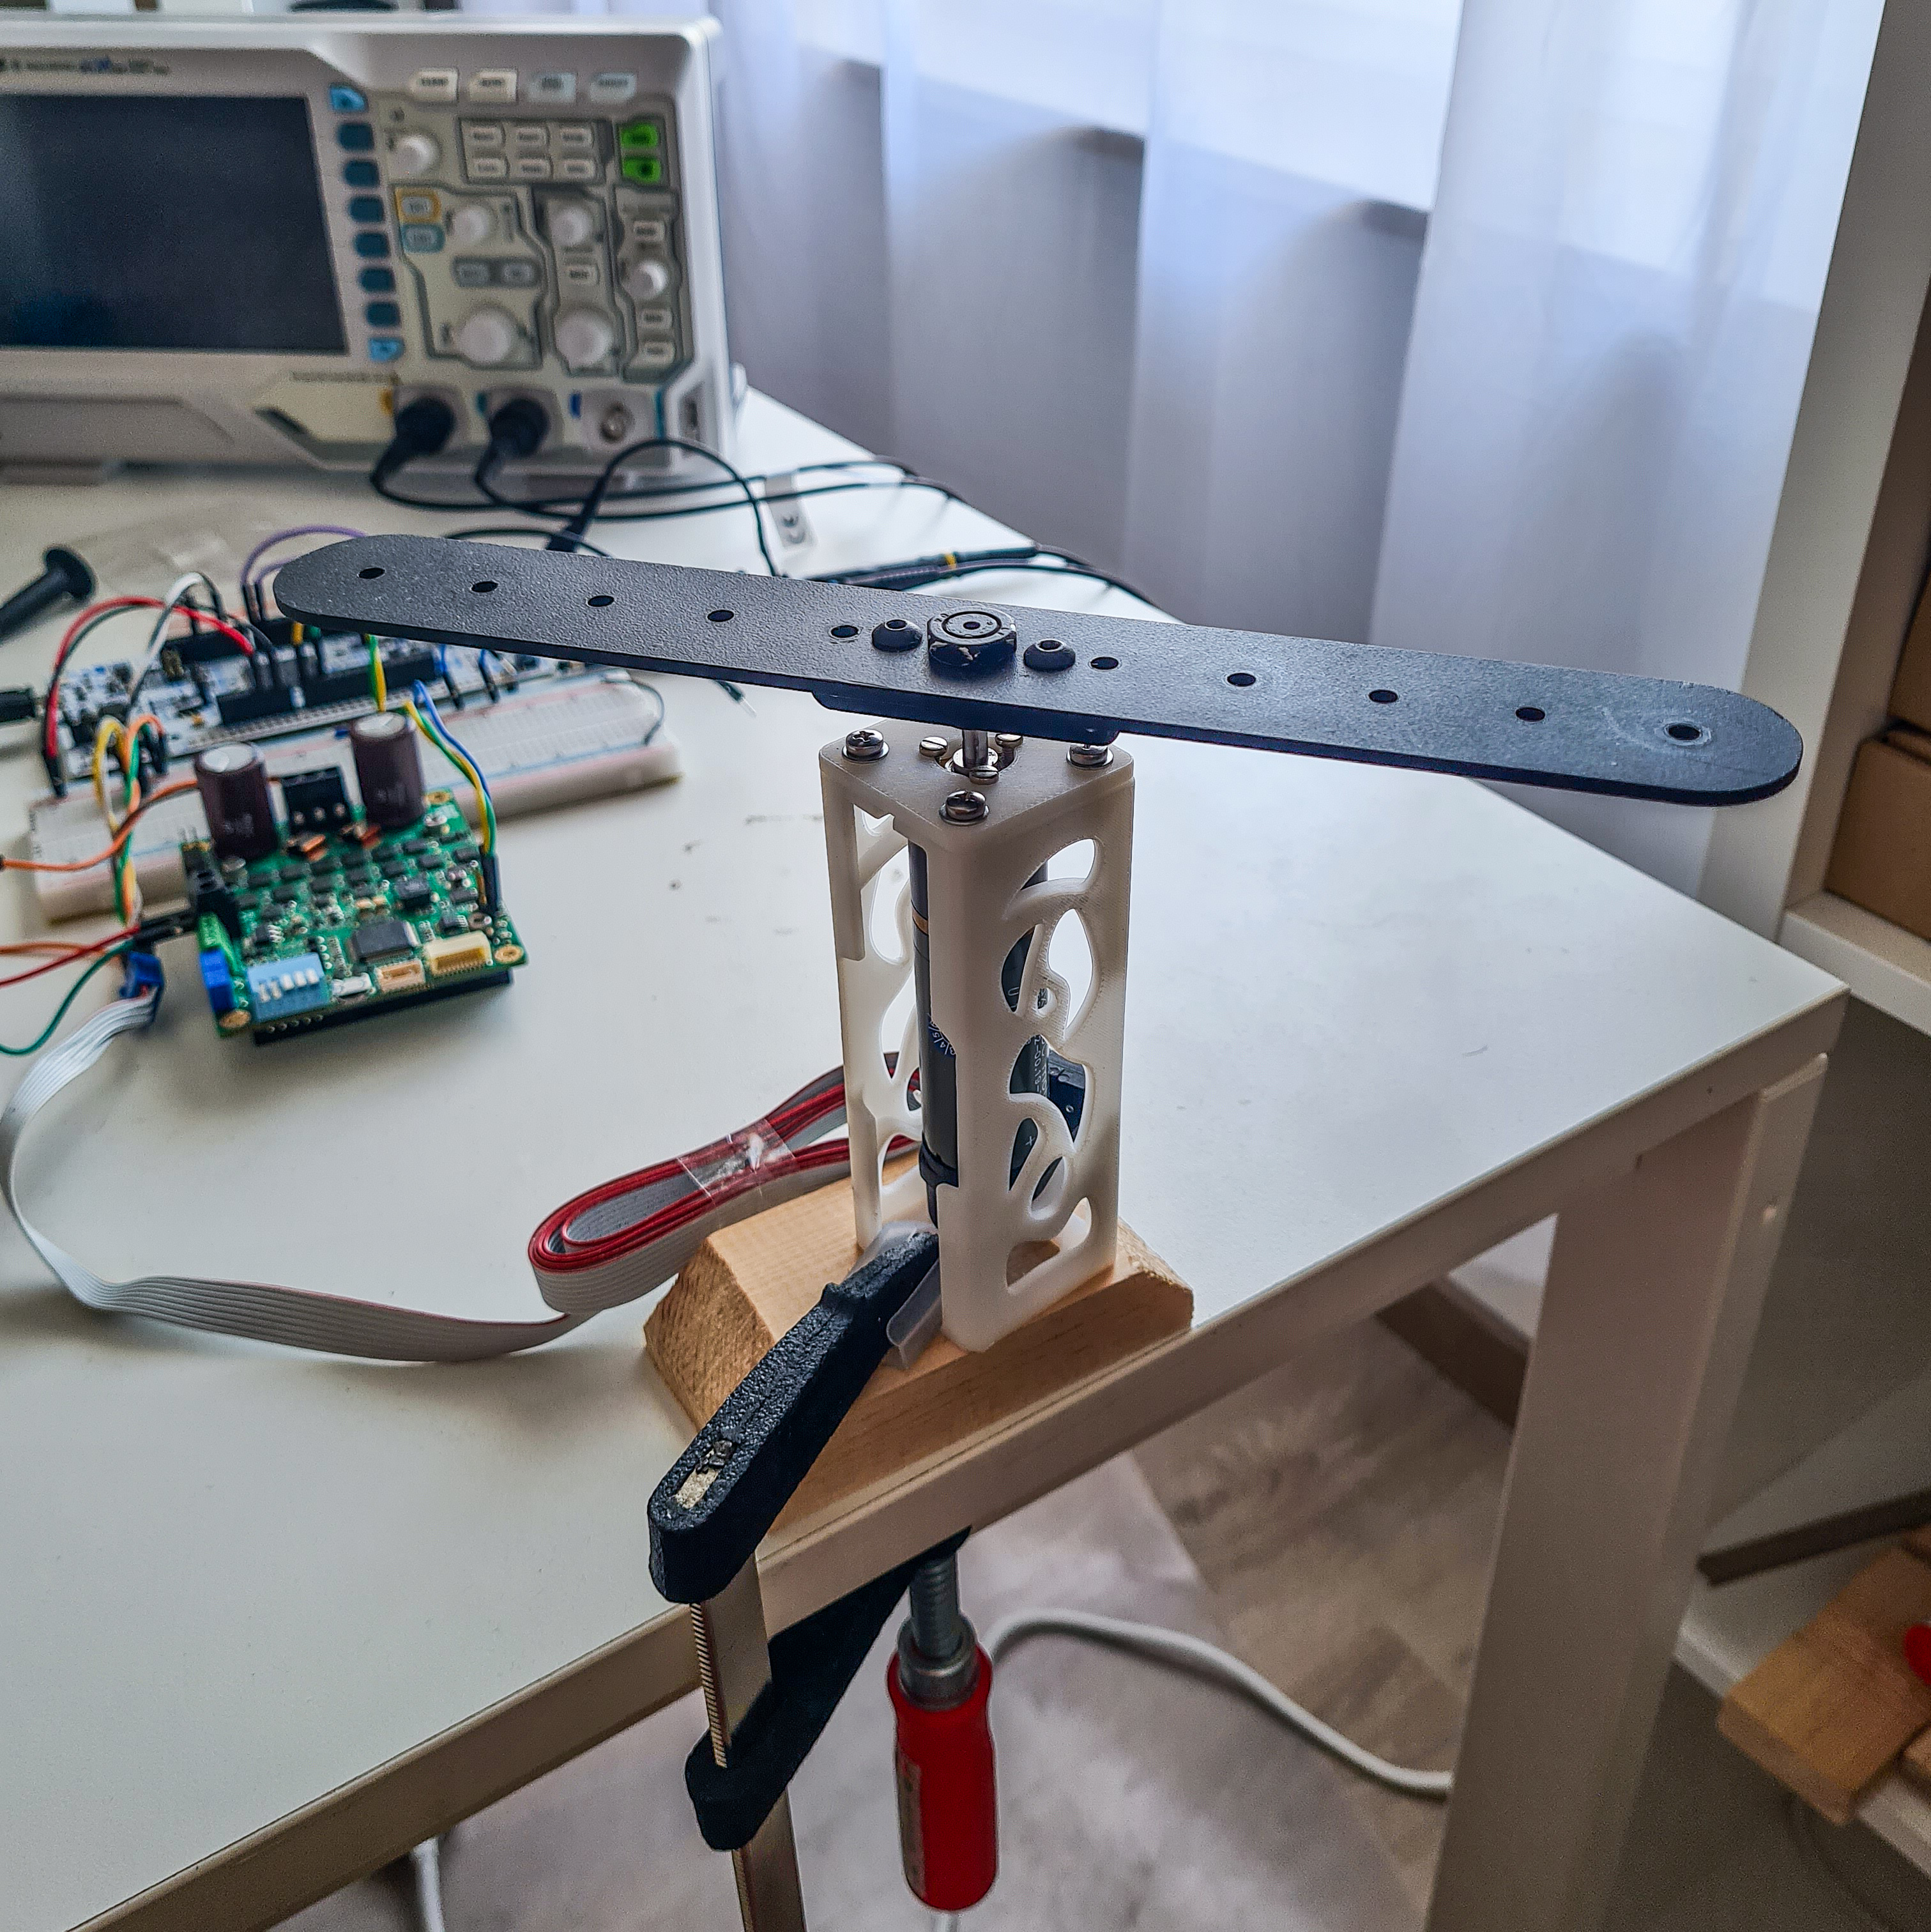
\includegraphics[width=14cm]{images/setup_experiment.jpg}
    \caption{Mérési összeállítás}\label{fig:setup_experiment}
    \end{center}
\end{figure}
A motorvezérlő egy SOLO UNO V2 32A típúsú univerzális vezérlő egység, mely egyenáramú kefés, kefe 
nélküli valamint PMSM és váltakozó áramú indukciós motorok vezérlésére is alkalmas 800W-ig. 
A kimenete változtatható frekvenciájú PWM jel. A kimeneti PWM vezérlő jel frekvenciája elméletben 80kHz-ig 
növelhető. A valóságban 75kHz-es beállítás felett automatikusan visszaugrott a frekvencia 20kHz-re, így 
a kísérletek során 75kHz volt a beállított frekvencia. CANopen és egy egyedi UART 
protokollon keresztül lehet kommunikálni az eszközzel. A kísérletek során a második opció lett alkalmazva.

% Alacsony induktivitású motoroknál, amilyen a kísérletben is felhasznált maxon motor, 
% a vezérlő jel átlagos amplitúdója és a motor nyomatéka között nem feltétlenül van lineáris kapcsolat. 
% Mivel ez egy alapvető feltétele a szabályozó alkalmazhatóságának, most ennek a jelenségnek a 
% részletesebb elemzése következik. A második fejezetben szereplő 
% \eqref{eq:rotor_dynamics} és \eqref{eq:armature_circuit} egyenletek alapján \dots

A szabályozó futtatását egy NUCLEO-F439ZI STMicrocontrollers fejlesztői panel végzi.
Alapvető feladatai:
\begin{itemize}
    \item Az inkrementális enkóder jelének olvasása a beépített számláló és időzítő periférián keresztül
    \item A szabályozó belső állapotának frissítése pontosan meghatározott időközönként.
    \item A szabályozó kimeneti referencia jelének továbbítása a motorvezérlőnek az előírt időkésés figyelembe vételével.
    \item A mérés állapotának felvétele és továbbítása a számítógép felé.
\end{itemize}
A szoftver egyszerűsített vázlata az \ref{fig:block_diagram_control_software}. ábrán látható. 
\begin{figure}[H]
    \begin{center}
    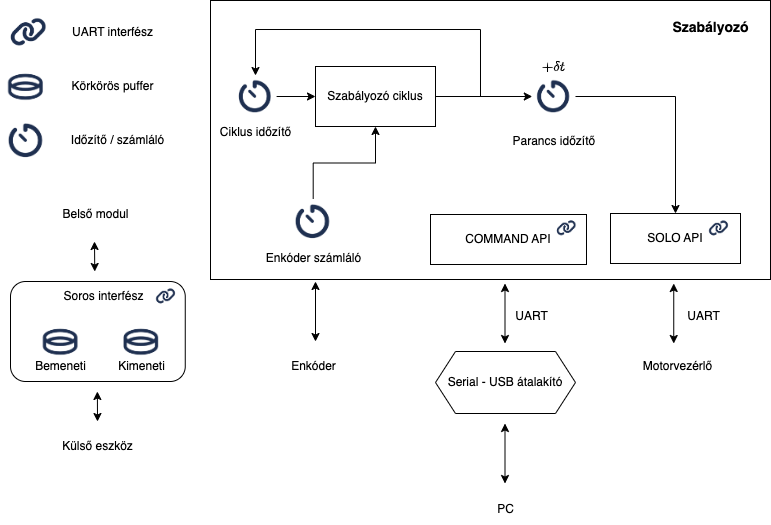
\includegraphics[width=14cm]{images/impedance_controler_software_diagram.png}
    \caption{Szabályozó szoftveres implementációjának egyszerűsített vázlata}\label{fig:block_diagram_control_software}
    \end{center}
\end{figure}
A szabályozó szoftvere egy C-ben írt program, mely az STMicrocontrollers STM32CubeIDE nevezetű 
fejlesztői környezetében készült. Minden időzítéssel kapcsolatos feladatot a beépített perifériák 
látnak el. A szabályozó ciklusa az adott méréshez előre meghatározott ciklusidő / időkésés figyelembe 
vételével periodikusan fut. Az implmentáció a \ref{chap:time_delay_stability}. fejezetben bemutatott 
digitalizált szabályozót követi. Mivel a motorvezérlőnek elküldött parancs meghatározásához szuukséges idő 
lényegesen rövidebb a méréseknél használt ciklusidőknél, egy külön időzítő felel a parancsok 
megfelelő késleltetéséért. A soros kommunikációhoz szükséges műveleteket soros interfész modulok 
végzik el. Minden interfész modul két körkörös pufferrel rendelkezik. Az egyik a kimenő, a másik 
a válasz üzeneteket tárolja. A pufferek és a UART perifériák közötti adatátvitelt a beépített DMA vezérlők 
valósítják meg. A mérés konfigurálása, nyomonkövetése, és az eredmények visszaküldése a számítógépre 
egy egyszerű protokoll segítségével történik. A protokoll felépítését a \ref{fig:measurement_protocol}. ábra 
mutatja. 
\begin{figure}[H]
    \begin{center}
    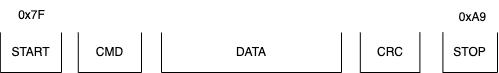
\includegraphics[width=14cm]{images/impedance_controler_software_measurement_protocol.png}
    \caption{A szabályozó kommunikációs protokollja}\label{fig:measurement_protocol}
    \end{center}
\end{figure}
A START, CMD és STOP egy byte hosszúak. A DATA mező fix hosszúságú, legtöbb esetben 4 byte, de a CMD mezőtől függ.
A CMD mező kódolja a parancs típusát. A CRC mező a CMD és DATA mezők alapján számított 8 bites CRC, a kommunikációs 
hibákból eredő félrekonfiguráció esélyének csökkentéséért felel. 

A mérésekhez felhasznált egyéb eszközök a \ref{tab:measurement_tools}. táblázatban találhatóak.
\begin{table}[H]
    \small\centering
    \caption{További mérési eszközök}\label{tab:measurement_tools}
    \tabcolsep=1pt
    \begin{tabular}{l>{~}l>{~}l>{\quad}rl}
        \toprule
        \multicolumn{1}{c}{Eszköz neve} & \multicolumn{1}{c}{Gyártója} & \multicolumn{1}{c}{Típusa} & \multicolumn{2}{c}{Precizitás} \\ \midrule
        Mérőórás tolómérő & Berger & 020701-0007 & \(\pm\)0.02 & mm \\
        Digitális oszcilloszkóp & Rigol & DS1202Z-E & 200 MHz / 1 & GSa/s \\
        DC laboratóriumi tápegység & UNI-T & UTP3315TFL-II & 0-30V \(\pm\) 10 mV, 0-5A \(\pm\) 1 & mA \\
        Digitális multiméter & MAXWELL & MX-25304 & \(\pm\)0.1 mV - 1 V, \(\pm\) 0.1 \(\mu\)A - 10 & mA \\
        \bottomrule
    \end{tabular}
\end{table}

\section{Paraméter identifikáció}
A szabályozó megfelelő működésének feltétele, hogy rendelkezésre álljanak a motor pontos paraméterei. 
Bár az adatlapokból több szükséges paraméter is kiolvasható, vannak paraméterek, amiket külön kellett 
meghatározni. Ilyen a motorra terhelésként ráhelyezett propeller tehetetlenségi nyomatéka és a viszkózus 
csillapítási tényező. A hajtómű áttétele, a rotor tehetetlenségi nyomatéka és a nyomatékállandó esetében 
az adatlapokban szereplő értékek lettek alkalmazva. A rotor ellenállása és a motorvezérlő motorra adott 
feszültségjelének amplitúdója és a vezérlő parancs közötti viszony külön lettek meghatározva. 

A rotor ellenállásának meghatározásához egy sor állandó feszültség lett kapcsolva a motorra 
lefogott állapotban, és a motor által felvett áram került feljegyzésre. A mért értékek a \ref{tab:resistance_measurement}. 
táblázatban találhatóak. 
\begin{table}[H]
    \small\centering
    \caption{Ellenállás mérés adatok}\label{tab:resistance_measurement}
    \tabcolsep=2pt
    \begin{tabular}{d{-1}>{~}d{-1}>{~}d{1}cl}
        \toprule
        \multicolumn{1}{c}{Kapocsfeszültség [V]} & \multicolumn{1}{c}{Felvett áram [A]} & \multicolumn{3}{c}{Ellenállás [\(\Omega\)]} \\ 
        \multicolumn{1}{c}{(mind \(\pm\) 0.01)} & \multicolumn{1}{c}{(mind \(\pm\) 0.01)} \\
        \midrule
        2.02 & 0.22 & 9.2 & \(\pm\) & 0.4 \\
        2.48 & 0.28 & 8.8 & \(\pm\) & 0.3 \\
        2.64 & 0.29 & 9.1 & \(\pm\) & 0.3 \\
        2.97 & 0.37 & 8.0 & \(\pm\) & 0.2 \\
        2.95 & 0.29 & 10.2 & \(\pm\) & 0.4 \\
        3.26 & 0.37 & 8.8 & \(\pm\) & 0.2 \\
        3.26 & 0.38 & 8.6 & \(\pm\) & 0.2 \\
        3.39 & 0.41 & 8.3 & \(\pm\) & 0.2 \\
        3.46 & 0.39 & 8.9 & \(\pm\) & 0.2 \\
        3.95 & 0.46 & 8.6 & \(\pm\) & 0.19 \\
        4.05 & 0.46 & 8.8 & \(\pm\) & 0.2 \\
        4.24 & 0.51 & 8.3 & \(\pm\) & 0.16 \\
        4.51 & 0.52 & 8.7 & \(\pm\) & 0.17 \\
        4.89 & 0.62 & 7.9 & \(\pm\) & 0.13 \\
        5.08 & 0.65 & 7.8 & \(\pm\) & 0.12 \\
        \midrule
        & \multicolumn{1}{r}{\(\bar R = \)} & 8.7 & \(\pm\) & 0.15 \\
        \bottomrule
    \end{tabular}
\end{table}
A mérések alapján kapott átlag bizonytalansága az egyes minták szórásából számított 
standard hiba. Ez az érték szignifikánsan eltér az adatlapban szereplő értéktől. A 
későbbi mérések alapján az adatlapban szereplő érték nem lett felhasználva.

A propeller tehetetlenségi nyomatéka lengési idők mérése alapján lett meghatározva. Egy 
adott ponton felfüggesztett merev test lengési periódusát, mely a gravitáció hatására 
szabadon leng egy síkban, a következő összefüggés írja le
\begin{equation}
    t_l = 2\pi\sqrt{\frac{I_\RM P}{mgd}},
\end{equation}
ahol \(I_\RM{P}\) a test tehetetlenségi nyomatéka, \(m\) a tömege, \(g\) a gravitációs állandó, 
és \(d\) a felfüggesztési pont és a test tömegözéppontja közötti távolság. 
Kifejezve a tehetetlenségi nyomatékot 
\begin{equation}
    I_\RM{P} = \frac{mgd}{4\pi^2}t^2_l,
\end{equation}
A mérési összeállítást szemlélteti a \ref{fig:propeller_pendulum}. ábra. Az 
előbbi formula relatíve kis kilengés esetén alkalmazható, így nagyjából 
10° volt a kezdeti kilengés.
\begin{figure}[H]
    \begin{center}
    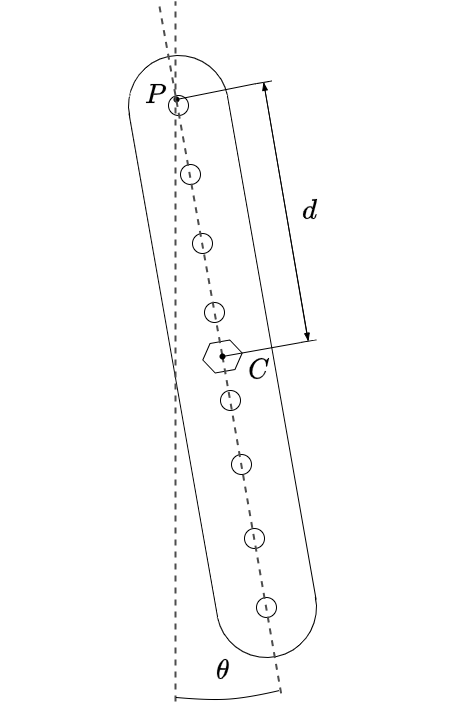
\includegraphics[height=12cm]{images/impedance_control_propeller.png}
    \caption{Felfüggesztett terhelés tehetetlenségi nyomaték méréshez}\label{fig:propeller_pendulum}
    \end{center}
\end{figure}
Minden mérés során harminc oda-vissza 
lengés ideje lett lemérve. Az eredmények az \ref{tab:propeller_period_measurement}. táblázatban találhatóak. A számított 
átlag a standard hibával együtt az utolsó sorban található. Az átlag már az egy periódusra számított 
időt mutatja.
\begin{table}[H]
    \small\centering
    \caption{Terhelés lengési idő mérési adatok}\label{tab:propeller_period_measurement}
    \tabcolsep=2pt
    \begin{tabular}{rd{-1}}
        \toprule
        \multicolumn{2}{c}{30 lengés periódus ideje [s]} \\ 
        \multicolumn{2}{c}{\(t_{30}\)} \\
        \midrule
        & 22.35 \\
        & 22.20 \\
        & 22.27 \\
        & 22.26 \\
        & 22.19 \\
        \midrule
        \multicolumn{1}{r}{\(\bar t_\RM l = \)} & \multicolumn{1}{c}{0.742 \(\pm\) 0.001} \\
        \bottomrule
    \end{tabular}
\end{table}
A későbbi mérésekhez a formulában szereplő felfüggesztéshez viszonyított tehetetlenségi 
nyomatékkal ellenben a tömegközéppontra számított tehetetlenségi nyomatékra van szükség. 
A Steiner-tétel alapján
\begin{equation}
    I_\RM{cm} = I_\RM{P} - md^2,
\end{equation}
A számításhoz szükséges összes paramétert a \ref{tab:propeller_measurement_summary}.
táblázat tartalmazza.
\begin{table}[H]
    \small\centering
    \caption{Terhelés tehetetlenségi nyomaték számítás adatok}\label{tab:propeller_measurement_summary}
    \tabcolsep=2pt
    \begin{tabular}{ccc}
        \toprule
        \multicolumn{1}{c}{Periódusidő [s]} & \multicolumn{1}{c}{Felfüggesztés távolsága [mm]} & \multicolumn{1}{c}{Propeller tömege [g]}\\ 
        \multicolumn{1}{c}{\(t_\RM l\)} & \multicolumn{1}{c}{\(d\)} & \multicolumn{1}{c}{\(m\)} \\
        \midrule
        0.742 \(\pm\) 0.001 & 110 \(\pm\) 1 & 43 \(\pm\) 1 \\
        \bottomrule
    \end{tabular}
\end{table}
A felfüggesztés és a propeller tömegközéppontja közötti távolság ugyan a \ref{tab:measurement_tools}. 
táblázatban szereplő tolómérővel lett meghatározva, a felfüggesztéshez használt drót rugalmassága miatt 
a felfüggesztési pont számomra nem egy jól definiált pont az eszköz precizitását figyelembe véve. Emiatt 
nagyobb a bizonytalanság ebben a paraméterben.

A gravitációs állandó étéke minden esetben \(g = 9.80 \frac{m}{s^2}\). További feltételezés, hogy a 
hibaszámítások során bizonytalansága elhanyagolhatónak tekinthető. Ezek alapján a propeller 
tehetetlenségi nyomatéka
\begin{equation}
    I_\RM{cm} = (1.26 \pm 0.05)\times10^{-4}~\RM{kg \cdot m^2}.
\end{equation}

A motorvezérlő linearitásának ellenőrzéséhez és a motorra eső feszültség pontosabb meghatározásához 
a motor kapocsfeszültsége és PWM vezérlő jel kitöltési tényezője is ki lett mérve különböző esetekben.
A mérési eredményeket a \ref{tab:driver_linearity_measurements}. táblázat tartalmazza. A két paraméter közötti kapcsolatot modellező 
egyenes lineáris regresszióval lett meghatározva. Ez az egyenes a mérési pontokkal együtt a \ref{fig:driver_linearity}.
ábrán látható.
\begin{table}[H]
    \small\centering
    \caption{Vezérlő jel és kapocsfeszültség mérések}\label{tab:driver_linearity_measurements}
    \tabcolsep=2pt
    \begin{tabular}{d{-1}>{~}d{-1}}
        \toprule
        \multicolumn{1}{c}{Kitöltési tényező [\%]} & \multicolumn{1}{c}{Kapocsfeszültség [V]} \\ 
        \multicolumn{1}{c}{\(f\) (mind \(\pm 0.1\))} & \multicolumn{1}{c}{\(V_\RM k\) (mind \(\pm 0.01\))} \\
        \midrule
        16.7 & 1.79 \\
        26.7 & 2.99 \\
        36.7 & 4.19 \\
        46.7 & 5.40 \\
        56.7 & 6.61 \\
        66.7 & 7.82 \\
        76.7 & 9.02 \\
        \bottomrule
    \end{tabular}
\end{table}
\begin{figure}[H]
    \begin{center}
    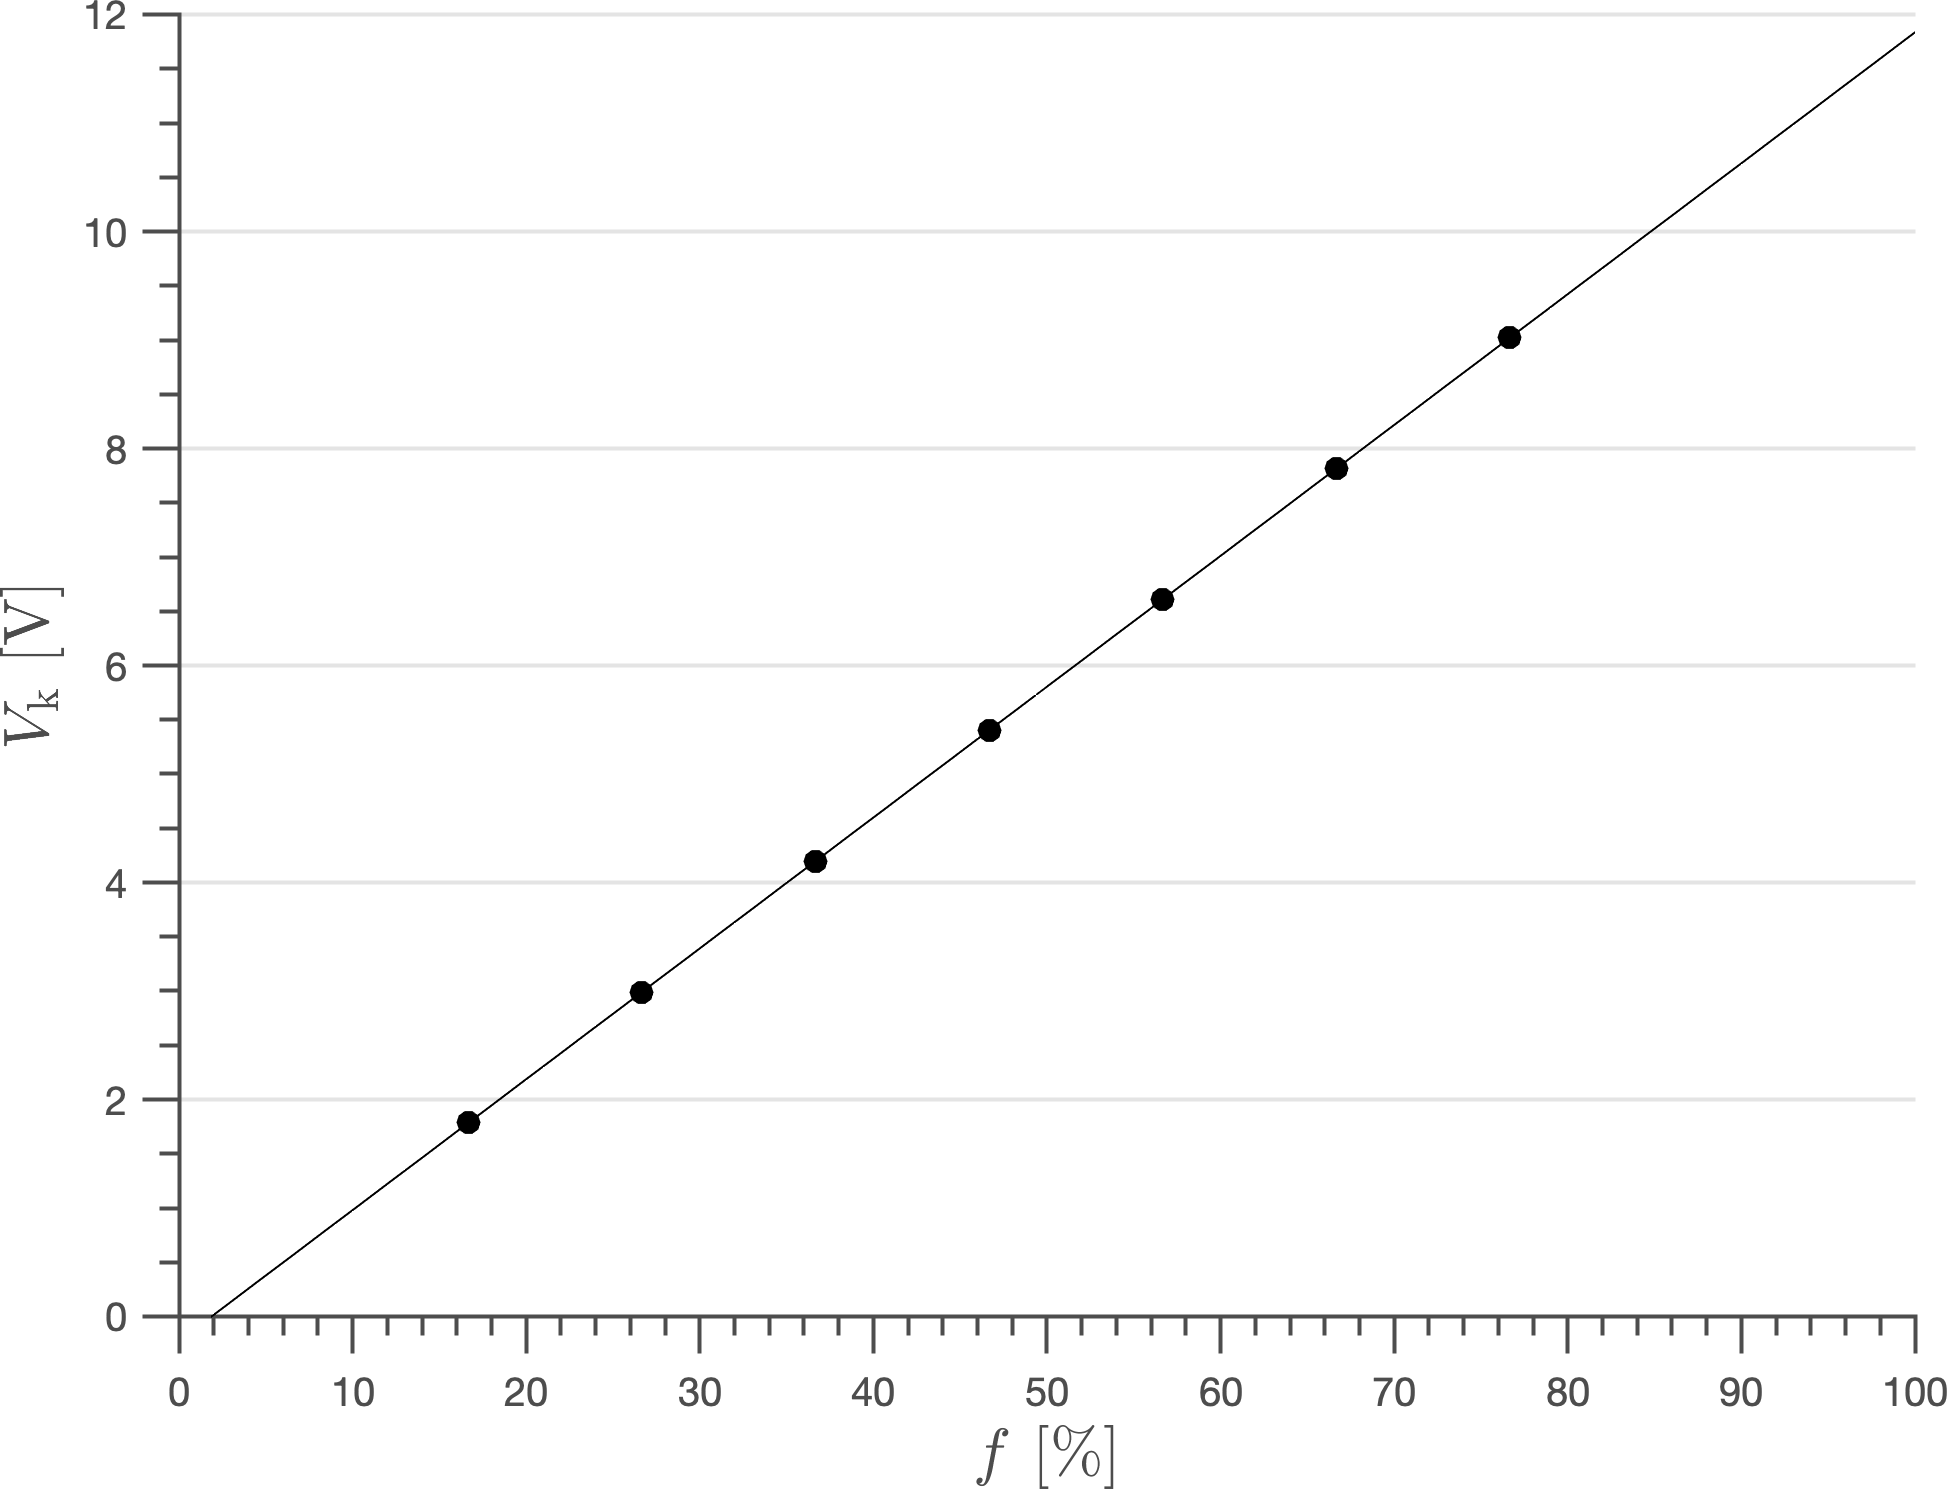
\includegraphics[width=14cm]{images/driver_linearity.png}
    \caption{Motor driver lineáritás vizsgálata}\label{fig:driver_linearity}
    \end{center}
\end{figure}
A hibasávok kis méretük miatt nem lettek ábrázolva. A motorvezérlő kimenetének linearitása 
jól látható.
A maximális feszültség ez alapján kcisit alacsonyabb a motorvezérlőnek bementként adott 
nominális 12V-os feszültségnél. Értéke \(V_\RM{max} = 11.835 \pm 0.005~[\RM V]\).

Az adatlapokban szereplő értékekkel kiegészítve a \eqref{eq:armature_circuit} és \eqref{eq:rotor_dynamics}
egyenletek alapján meghatározható a modell viszkózus csillapítási állandója, ha a motor állandósult 
állapotában mért sebessége is meghatározható. Ennek a mérésnek az eredményeit foglalja össze az \ref{tab:speed_profile}.
táblázat. A lineáris regresszióval illesztett egyenes és a mérési pontok az \ref{fig:speed_profile}. ábrán látható. 
\begin{table}[H]
    \small\centering
    \caption{Motor végsebesség és kapocsfeszültség mérések}\label{tab:speed_profile}
    \tabcolsep=2pt
    \begin{tabular}{d{-1}>{~}d{-1}}
        \toprule
        \multicolumn{1}{c}{Kapocsfeszültség [V]} & \multicolumn{1}{c}{Rotor sebessége [rad/s]} \\ 
        \multicolumn{1}{c}{\(V_\RM k\) (mind \(\pm 0.01\))} & \multicolumn{1}{c}{\(\omega_\RM r\) (mind \(\pm 0.1\))} \\
        \midrule
        1.18 & 36.3 \\
        1.38 & 54.7 \\
        1.58 & 68.1 \\
        1.78 & 79.9 \\
        1.97 & 94.3 \\
        2.17 & 106.6 \\
        2.37 & 120.0 \\
        2.56 & 133.1 \\
        2.76 & 146.5 \\
        2.96 & 160.3 \\
        3.16 & 173.7 \\
        3.35 & 187.6 \\
        3.55 & 199.1 \\
        3.75 & 211.8 \\
        3.94 & 224.7 \\
        4.14 & 237.2 \\
        4.34 & 250.4 \\
        4.54 & 262.4 \\
        4.73 & 274.7 \\
        4.93 & 287.3 \\
        5.13 & 299.7 \\
        5.33 & 311.8 \\
        5.52 & 324.3 \\
        5.72 & 336.4 \\
        5.92 & 349.0 \\
        6.11 & 361.6 \\
        6.31 & 374.1 \\
        6.51 & 386.2 \\
        6.71 & 397.8 \\
        6.90 & 410.0 \\
        7.10 & 420.8 \\
        7.30 & 432.1 \\
        7.50 & 445.3 \\
        7.69 & 456.5 \\
        7.89 & 469.2 \\
        8.09 & 479.9 \\
        8.28 & 491.1 \\
        8.48 & 502.2 \\
        8.68 & 514.1 \\
        8.88 & 526.6 \\
        9.07 & 537.2 \\
        9.27 & 549.2 \\
        9.47 & 560.4 \\
        9.67 & 571.7 \\
        9.86 & 582.9 \\
        \bottomrule
    \end{tabular}
\end{table}
\begin{figure}[H]
    \begin{center}
    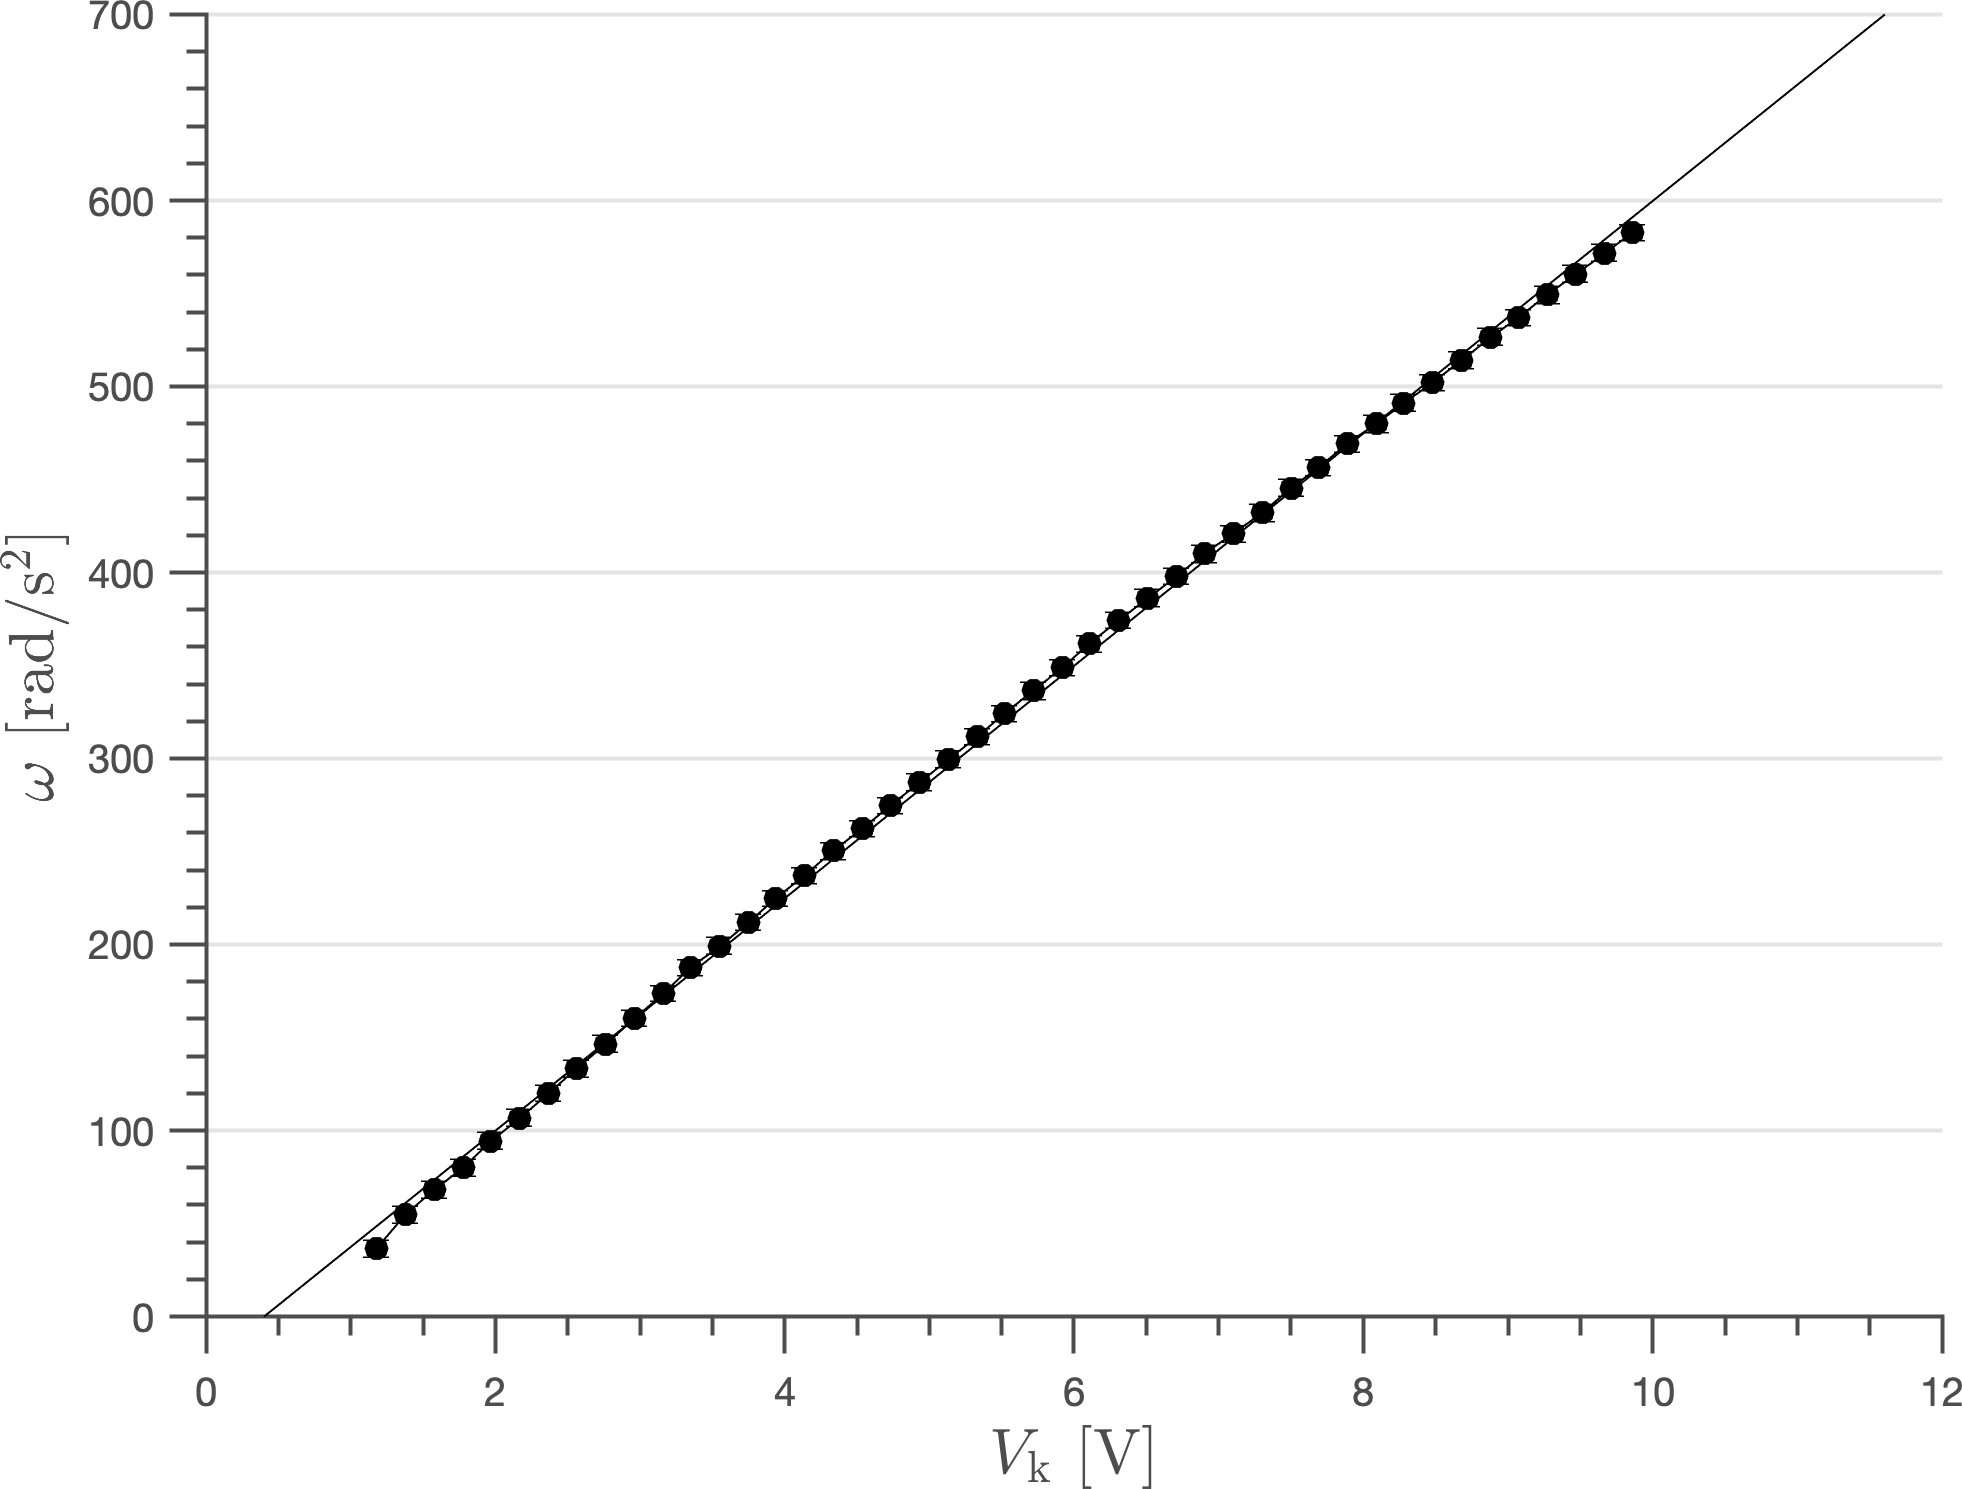
\includegraphics[width=14cm]{images/speed_profile.png}
    \caption{Motor végsebesség és kapocsfeszültség közötti kapcsolat}\label{fig:speed_profile}
    \end{center}
\end{figure}
A viszkózus csillapítási együtthatóra kapott becslés így
\begin{equation}
    B_\RM m = \frac{K_\RM m}{R}\left(\frac{1}{\alpha_\RM s} - K_\RM m\right),
\end{equation}
ahol \(\alpha_s\) az állandósult sebesség és a kapocsfeszültség közötti kapcsolatot 
leíró lineáris regresszióból kapott egyenes meredeksége. Minden paraméter ismert bizonytalanságukkal 
együtt. A végleges becslés
\begin{equation}
    B_\RM m = (1.1 \pm 0.1)\times 10^{-6}~\RM{kg\cdot m^2\cdot s^{-1}}.
\end{equation}

\section{Eredmények}
A motorparaméterek meghatározása után lehetőség nyílt a valós rendszer és a szimuláció összehasonlítására.
Az egységugrásra adott válasz összehasonlítását a szimulált digitális szabályozóval és a beállított impedancia modellel 
az \ref{fig:step_response_experiment0005}. ábra mutatja. Az időkésés \(\tau = 5~\RM{ms}\). Az impedancia modell paraméterei 
\(M_\RM e = 7.35 \times 10^{-6}~\RM{kg \cdot m^2}\), \(B_\RM e = 2.43 \times 10^{-4}~\RM{kg \cdot m^2 \cdot s^{-1}}\),
\(K_\RM e = 4.20 \times 10^{-3}~\RM{kg \cdot m^2 \cdot s^{-2}}\). Ezek egy enyhén alulcsillapított rendszer paraméterei, 
200 ms beállási idővel és ~0.7-es relatív csillapítási hányadossal. Jól látszik, hogy a végérték közelében 
a rendszer eltér a modellezett digitális szabályozótól, de kezdeti viselkedése és a végérték tekintetében is megfelel.
\begin{figure}[H]
    \begin{center}
    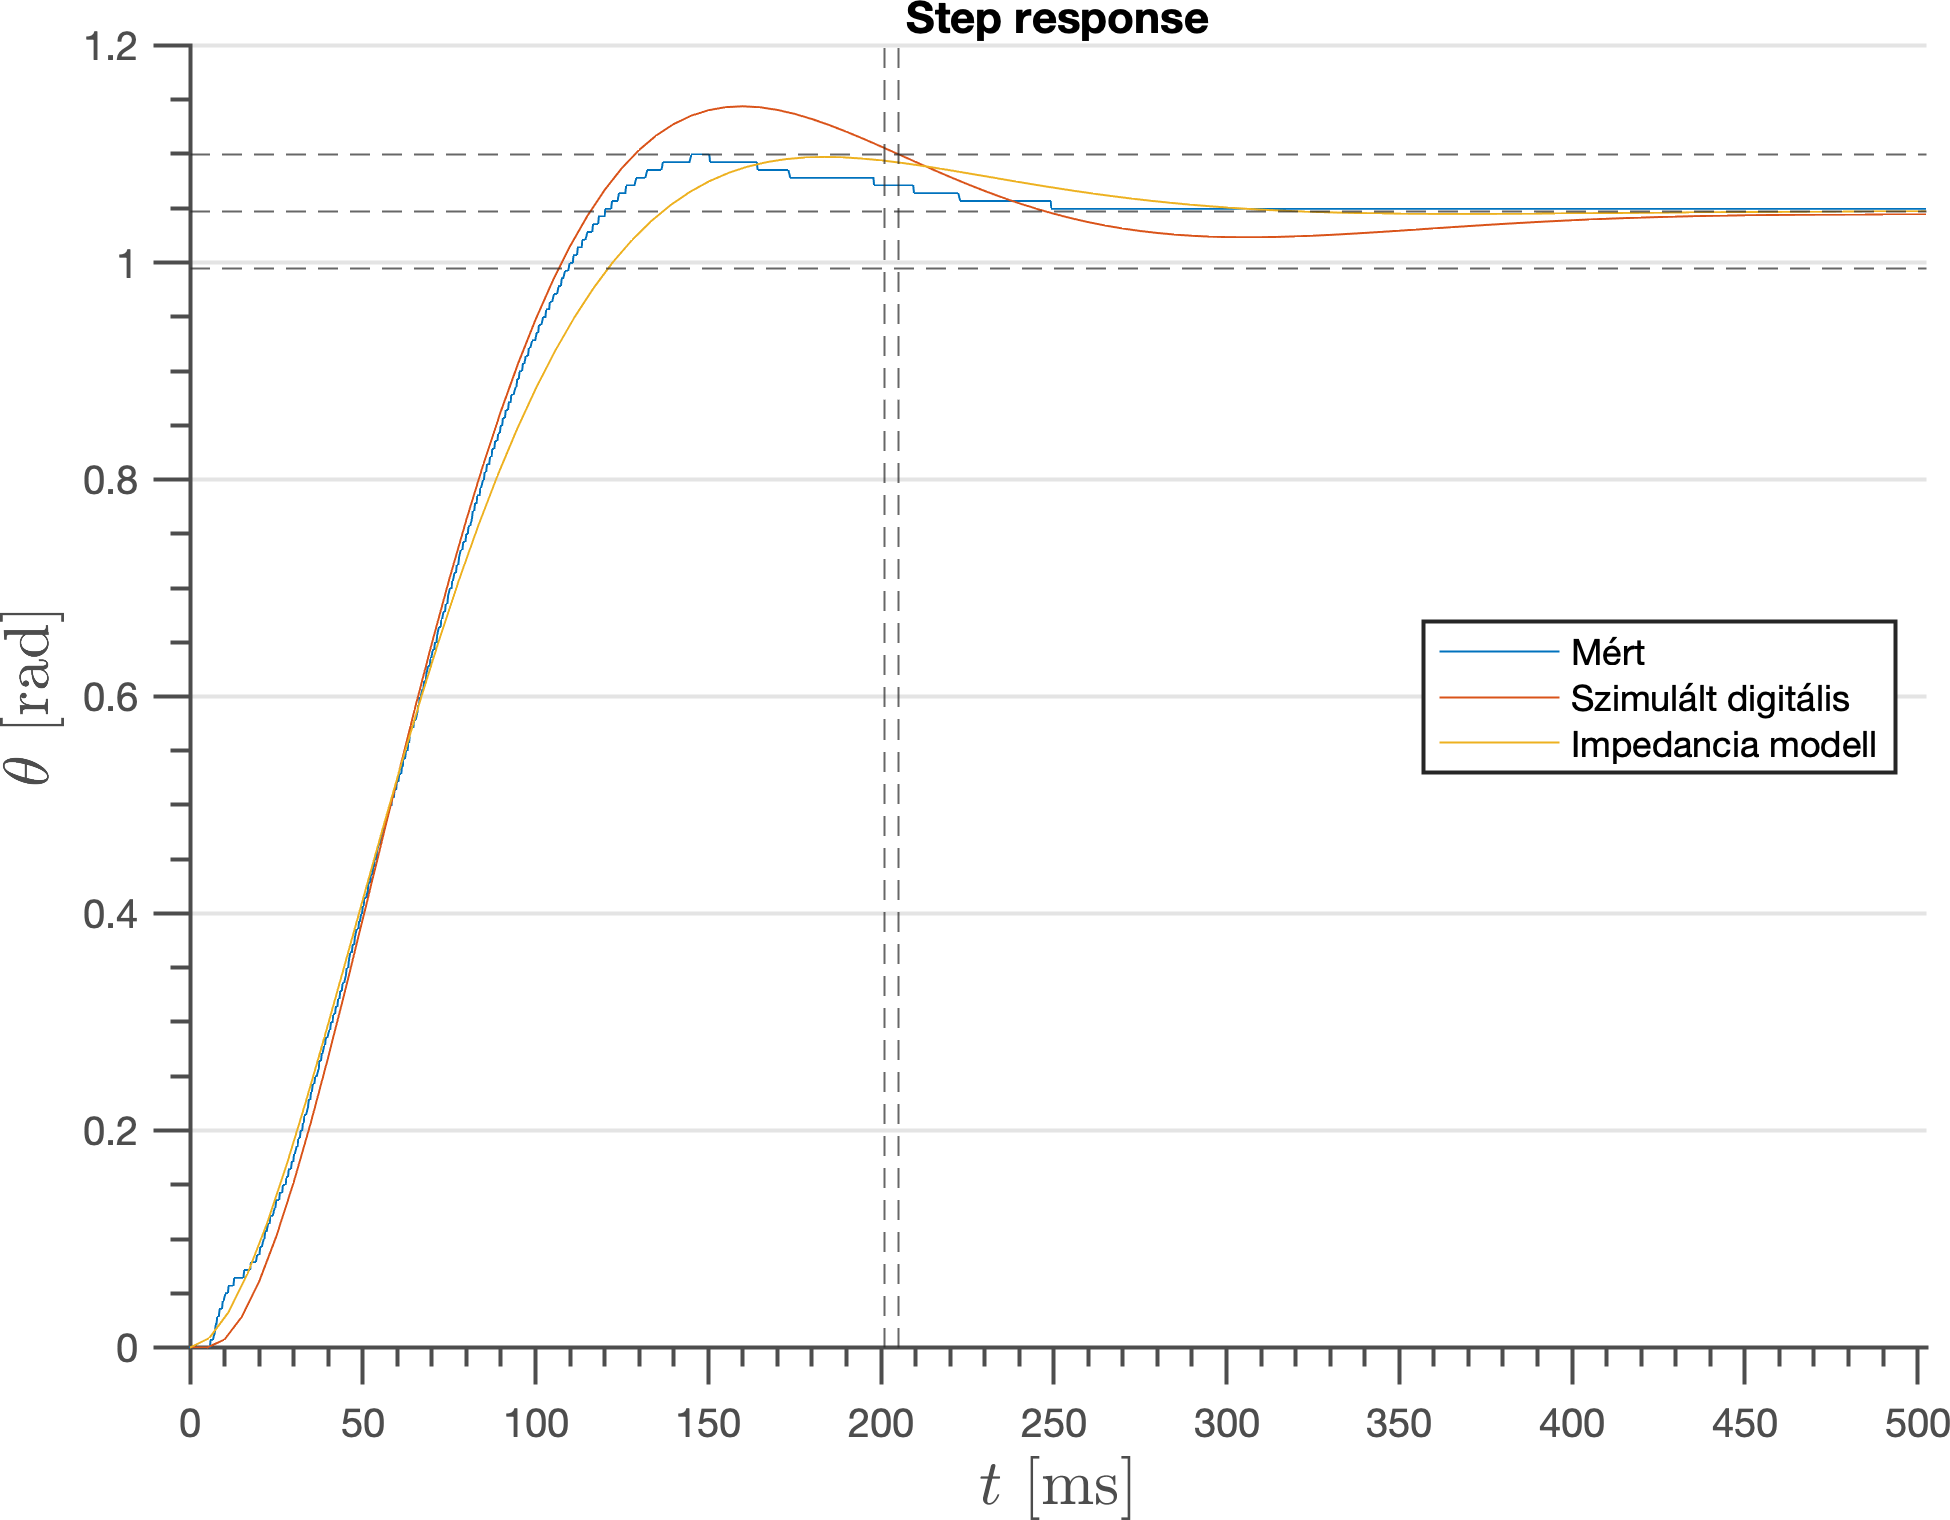
\includegraphics[width=\textwidth]{images/step_response_experiment0005.png}
    \caption{Egységugrás válasz \(\theta_\RM r = \pi/3\) referencia szögállásra, 5 ms időkéséssel és 95\%-os toleranciasávval}\label{fig:step_response_experiment0005}
    \end{center}
\end{figure}
A mért szögelfordulás közvetlenül az enkóder jeléből lett meghatározva. A mintavételezési frekvencia közel 4kHz volt 
minden esetben. 

A teljes stabilitástérkép felderítéséhez a beállási idő vizsgálata tűnt a legjobb módszernek. A \ref{fig:time_delay_stab_map_discrete_diff}. 
ábrához hasonlóan az új motorparaméterekkel meghatározott stabilitástérkép egy része látható az \ref{fig:stab_map_001}. ábrán.
Azonban itt a vízszintes tengelyen az elvárt impedancia modell sajátkörfrekvenciája \(\omega_\RM 0\), a függőleges 
tengelyen pedig az elvárt tehetetlenségi nyomatékhoz viszonyított viszkózus csillapítási állandó \(b_\RM e\) található.
Fontos eltérés még, hogy megjelennek a elvárt beállási idők kontúrjai, melyek jobbról közel vízszintesen indulnak, 
majd a 45°-os átló előtt nem sokkal a függőlegestől enyhén jobbra haladnak tovább, a térkép felső széle felé. 
Az origóból induló egyenesek az állandó relatív csillapítási hányadosokat jelölik. A tengelyek osztásai éppen olyanok, 
hogy a kritikus csillapítási hányadost az egységnyi meredekségű egyenes jelöli. A színezett tartomány az aszimptotikusan 
stabil paraméterkombinációkat jelöli. A különböző színek és a közöttük lévő kontúrok itt is a digitális szabályozó modell és az 
impedancia modell beállási ideje közötti relatív hibát mutatja, azonban a színskála \(\pm 10\%\) hiba között mozog. 
Tehát a méretes bordó terület 10\% hiba feletti eltérést, a lila -10\% alatti, míg a zöld terület 0-2\% hiba közötti 
eltérést jelöl. Ezeken a határokon belül minden színváltás \(\pm2\%\)-al eltérő hibát mutat. A 10\% feletti 
területen belüli kontúrok még viszonyításként megmutatják a 25\%, 50\% és 100\%-os eltéréseket is. 
Az \ref{fig:stab_map_0005}. és \ref{fig:stab_map_00025}. ábrák a csökkenő időkésés hatását szemléltetik. 
A stabil tartomány megnövekszik, ami az alacsonyabb hibával rendelkező területek 
megnövekedését eredményezi. Ez lehetővé teszi, azonos hiba mellett, egy gyorsabb rendszer működtetését. 
\begin{figure}[H]
    \begin{center}
    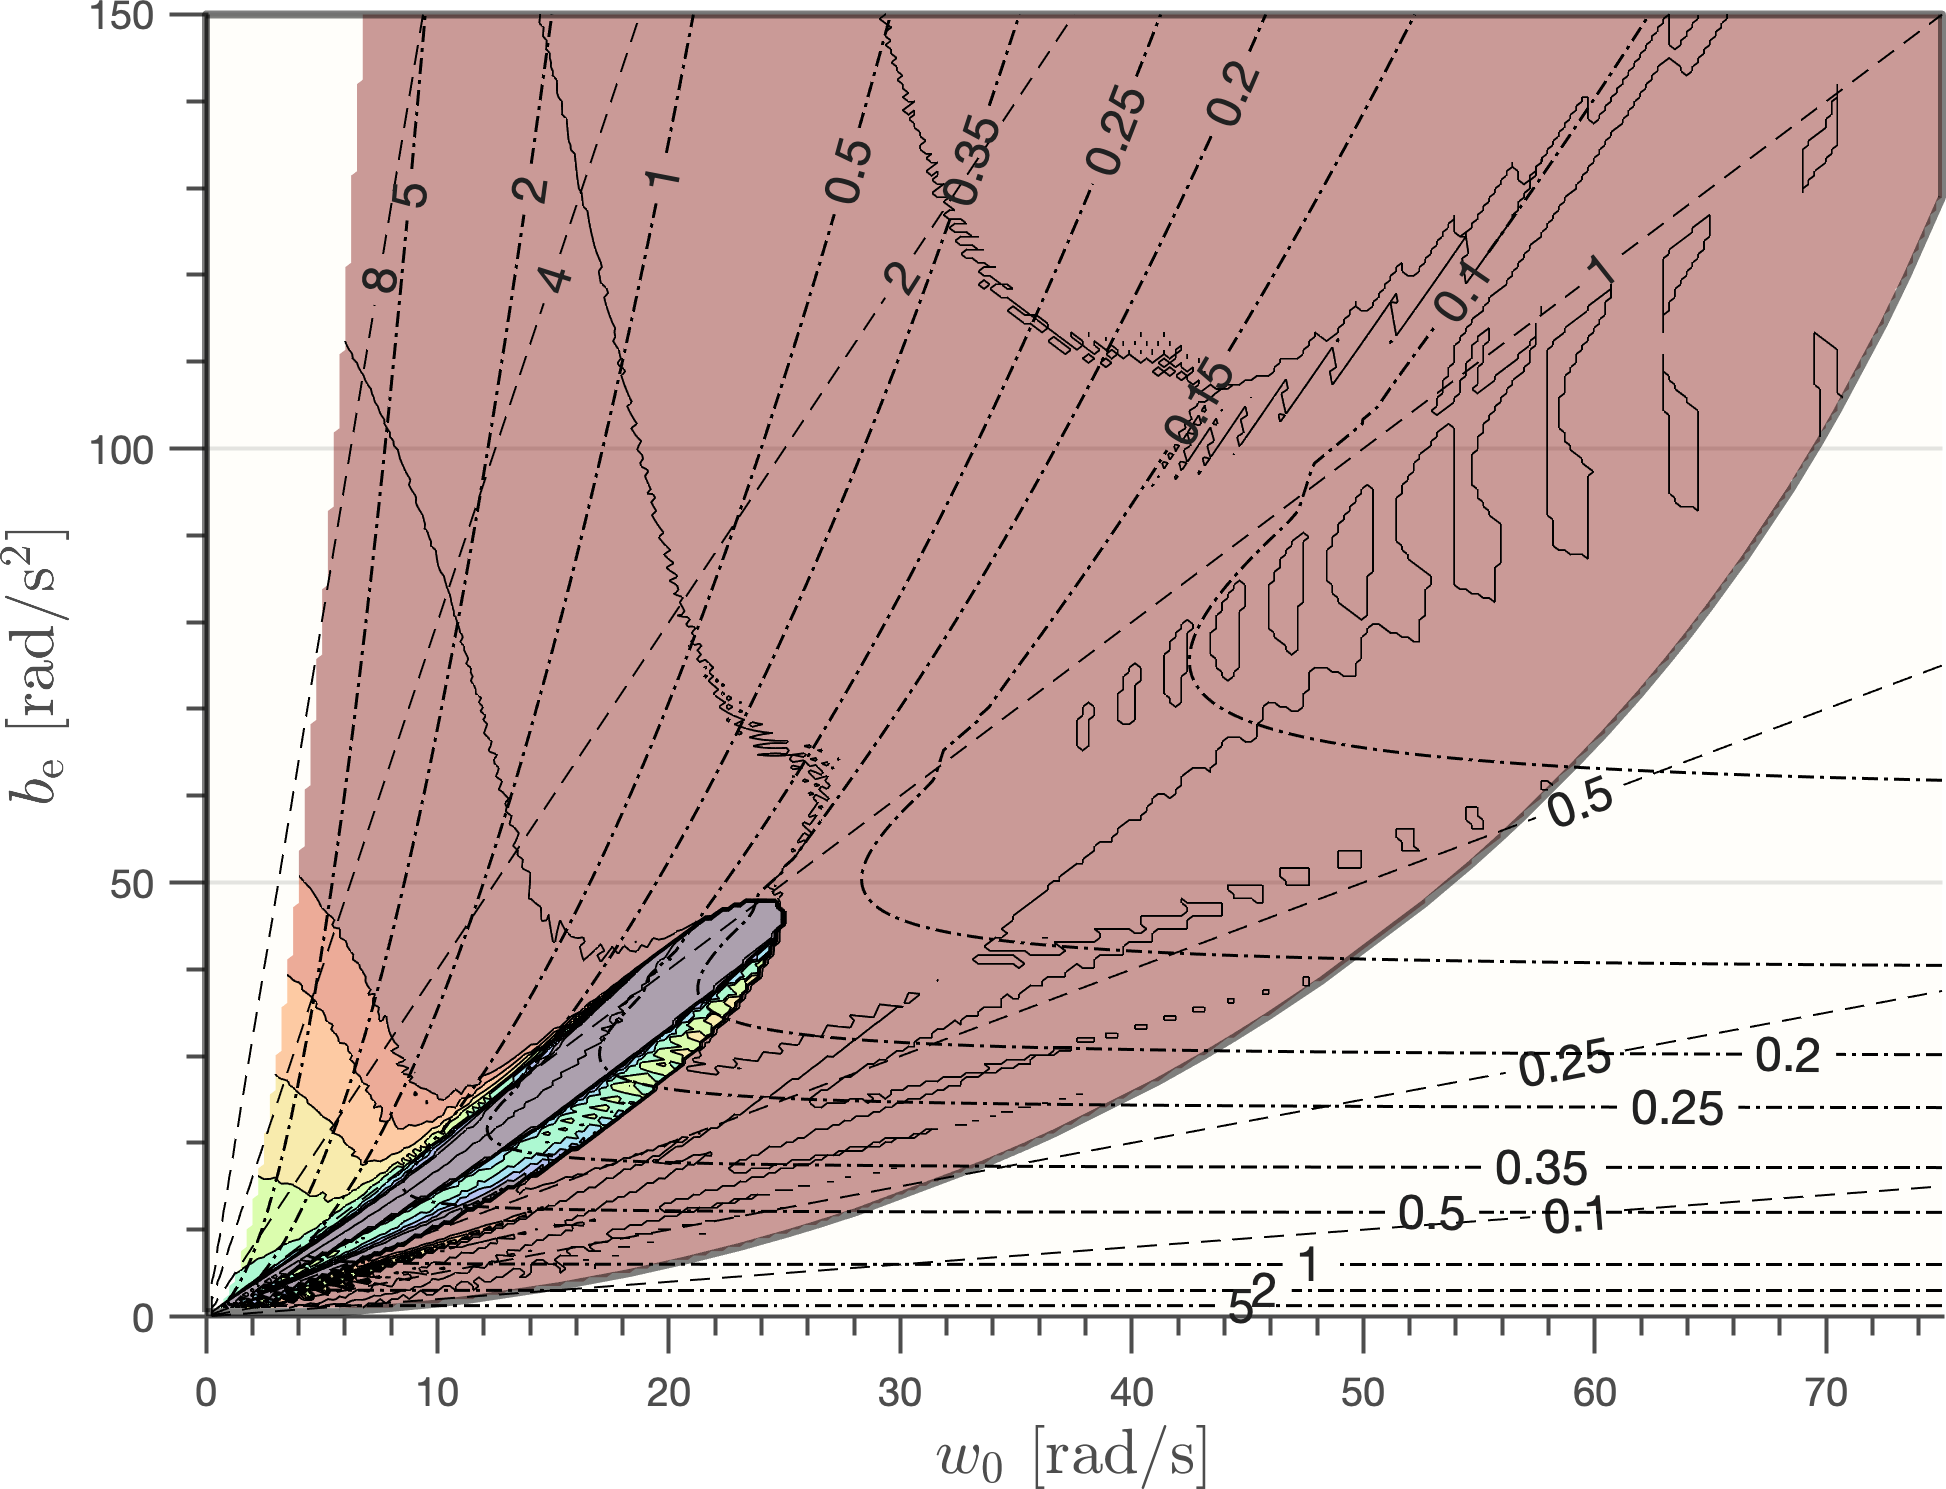
\includegraphics[width=14cm]{images/stab_map_001.png}
    \caption{Stabilitástérkép 10ms időkéséssel}\label{fig:stab_map_001}
    \end{center}
\end{figure}
\begin{figure}[H]
    \begin{center}
    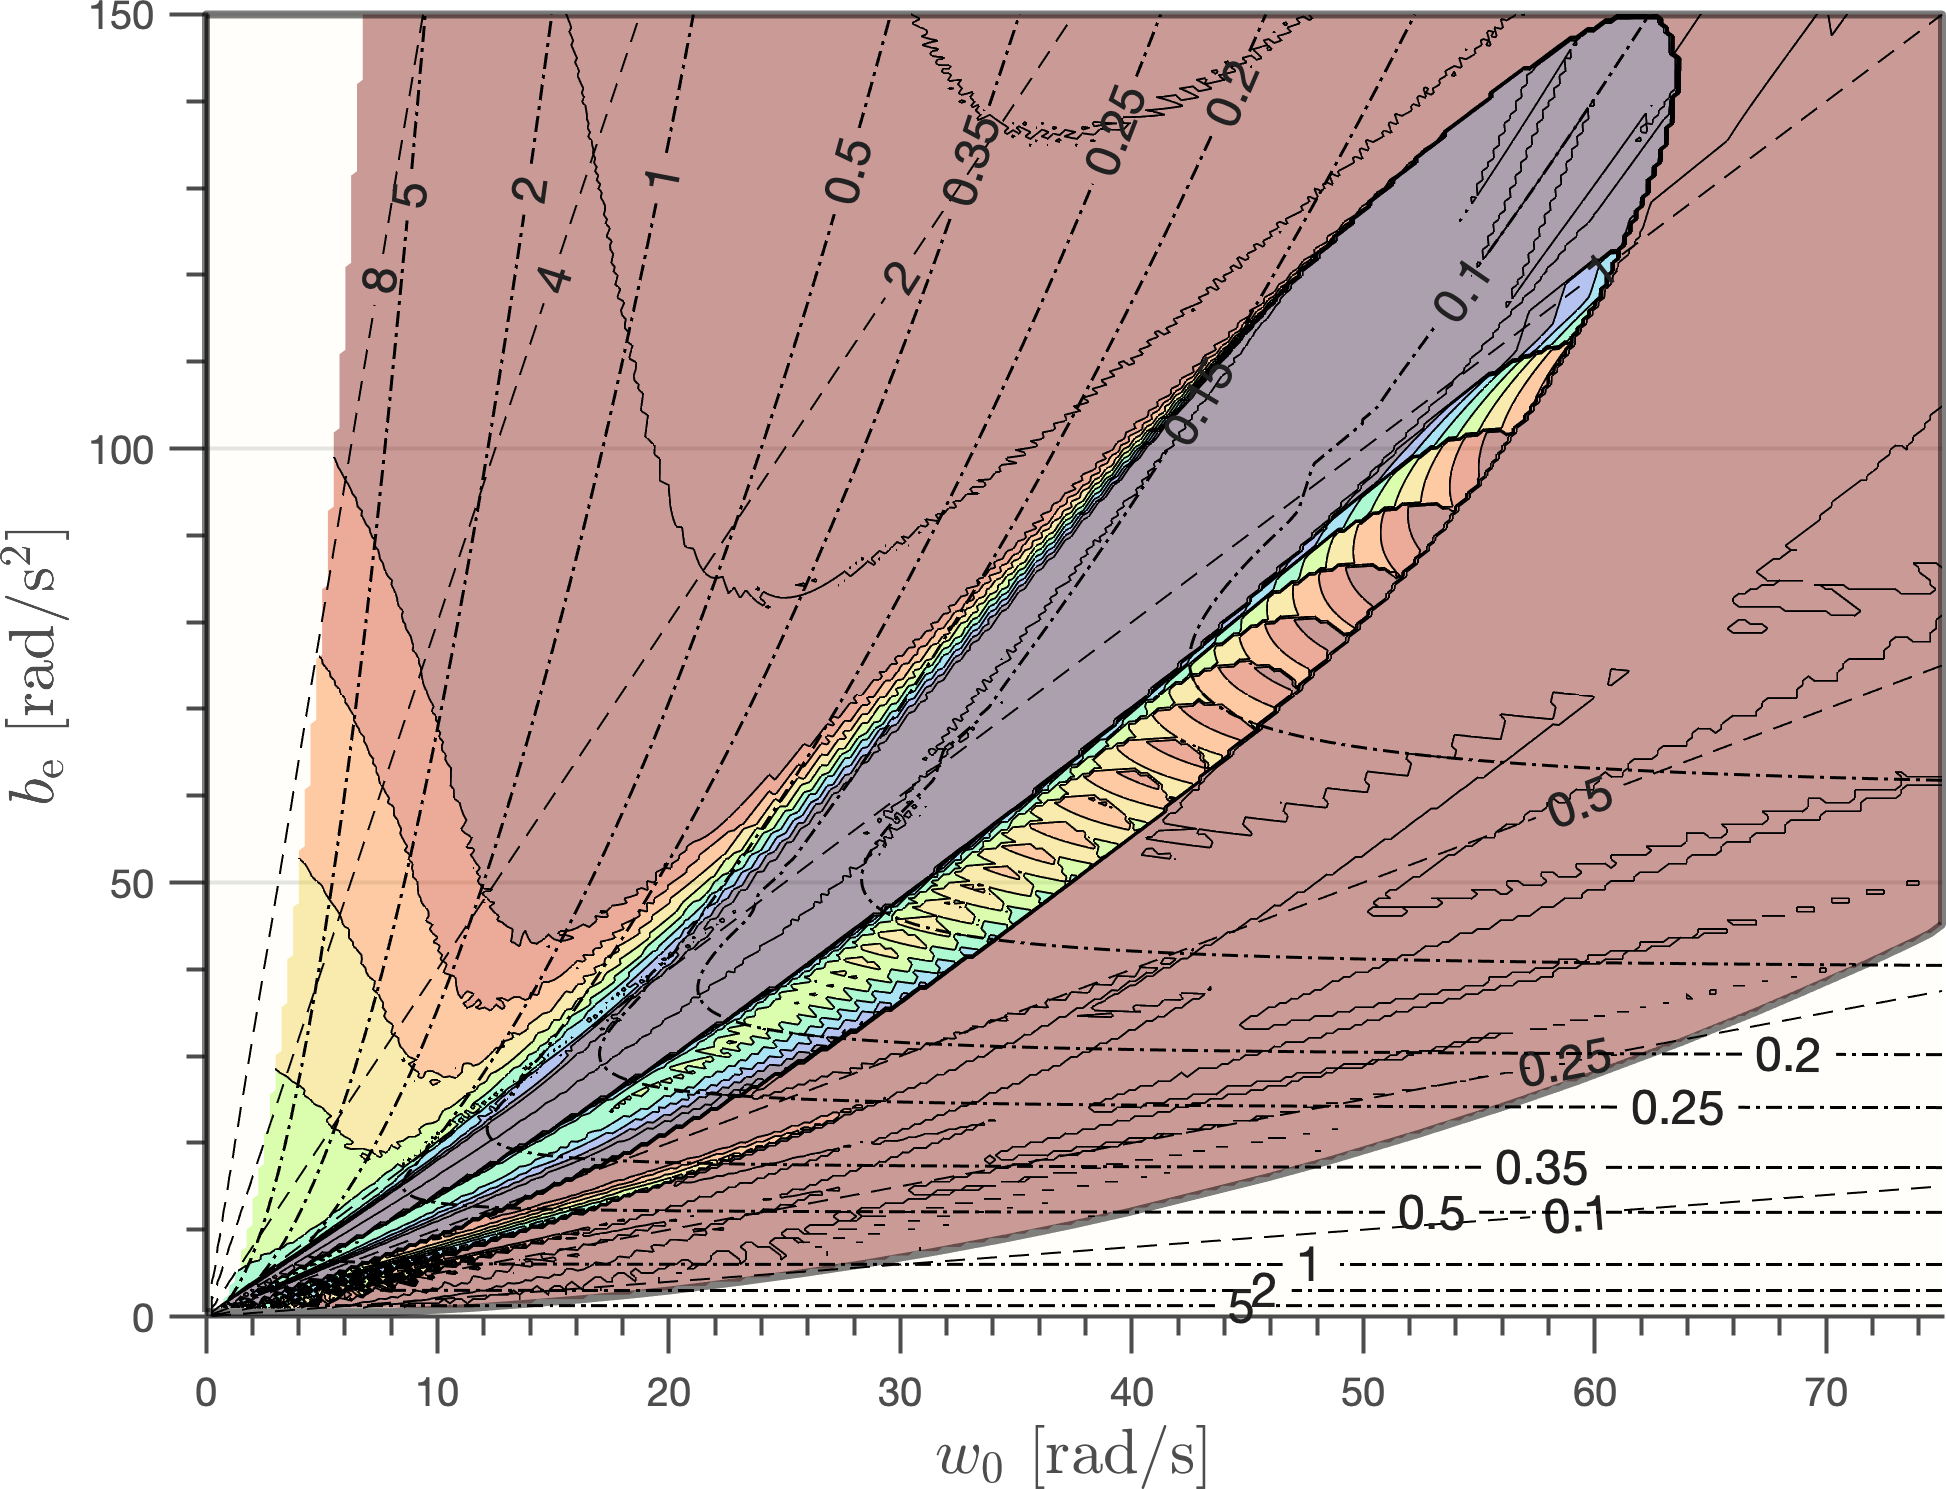
\includegraphics[width=14cm]{images/stab_map_0005.png}
    \caption{Stabilitástérkép 5ms időkéséssel}\label{fig:stab_map_0005}
    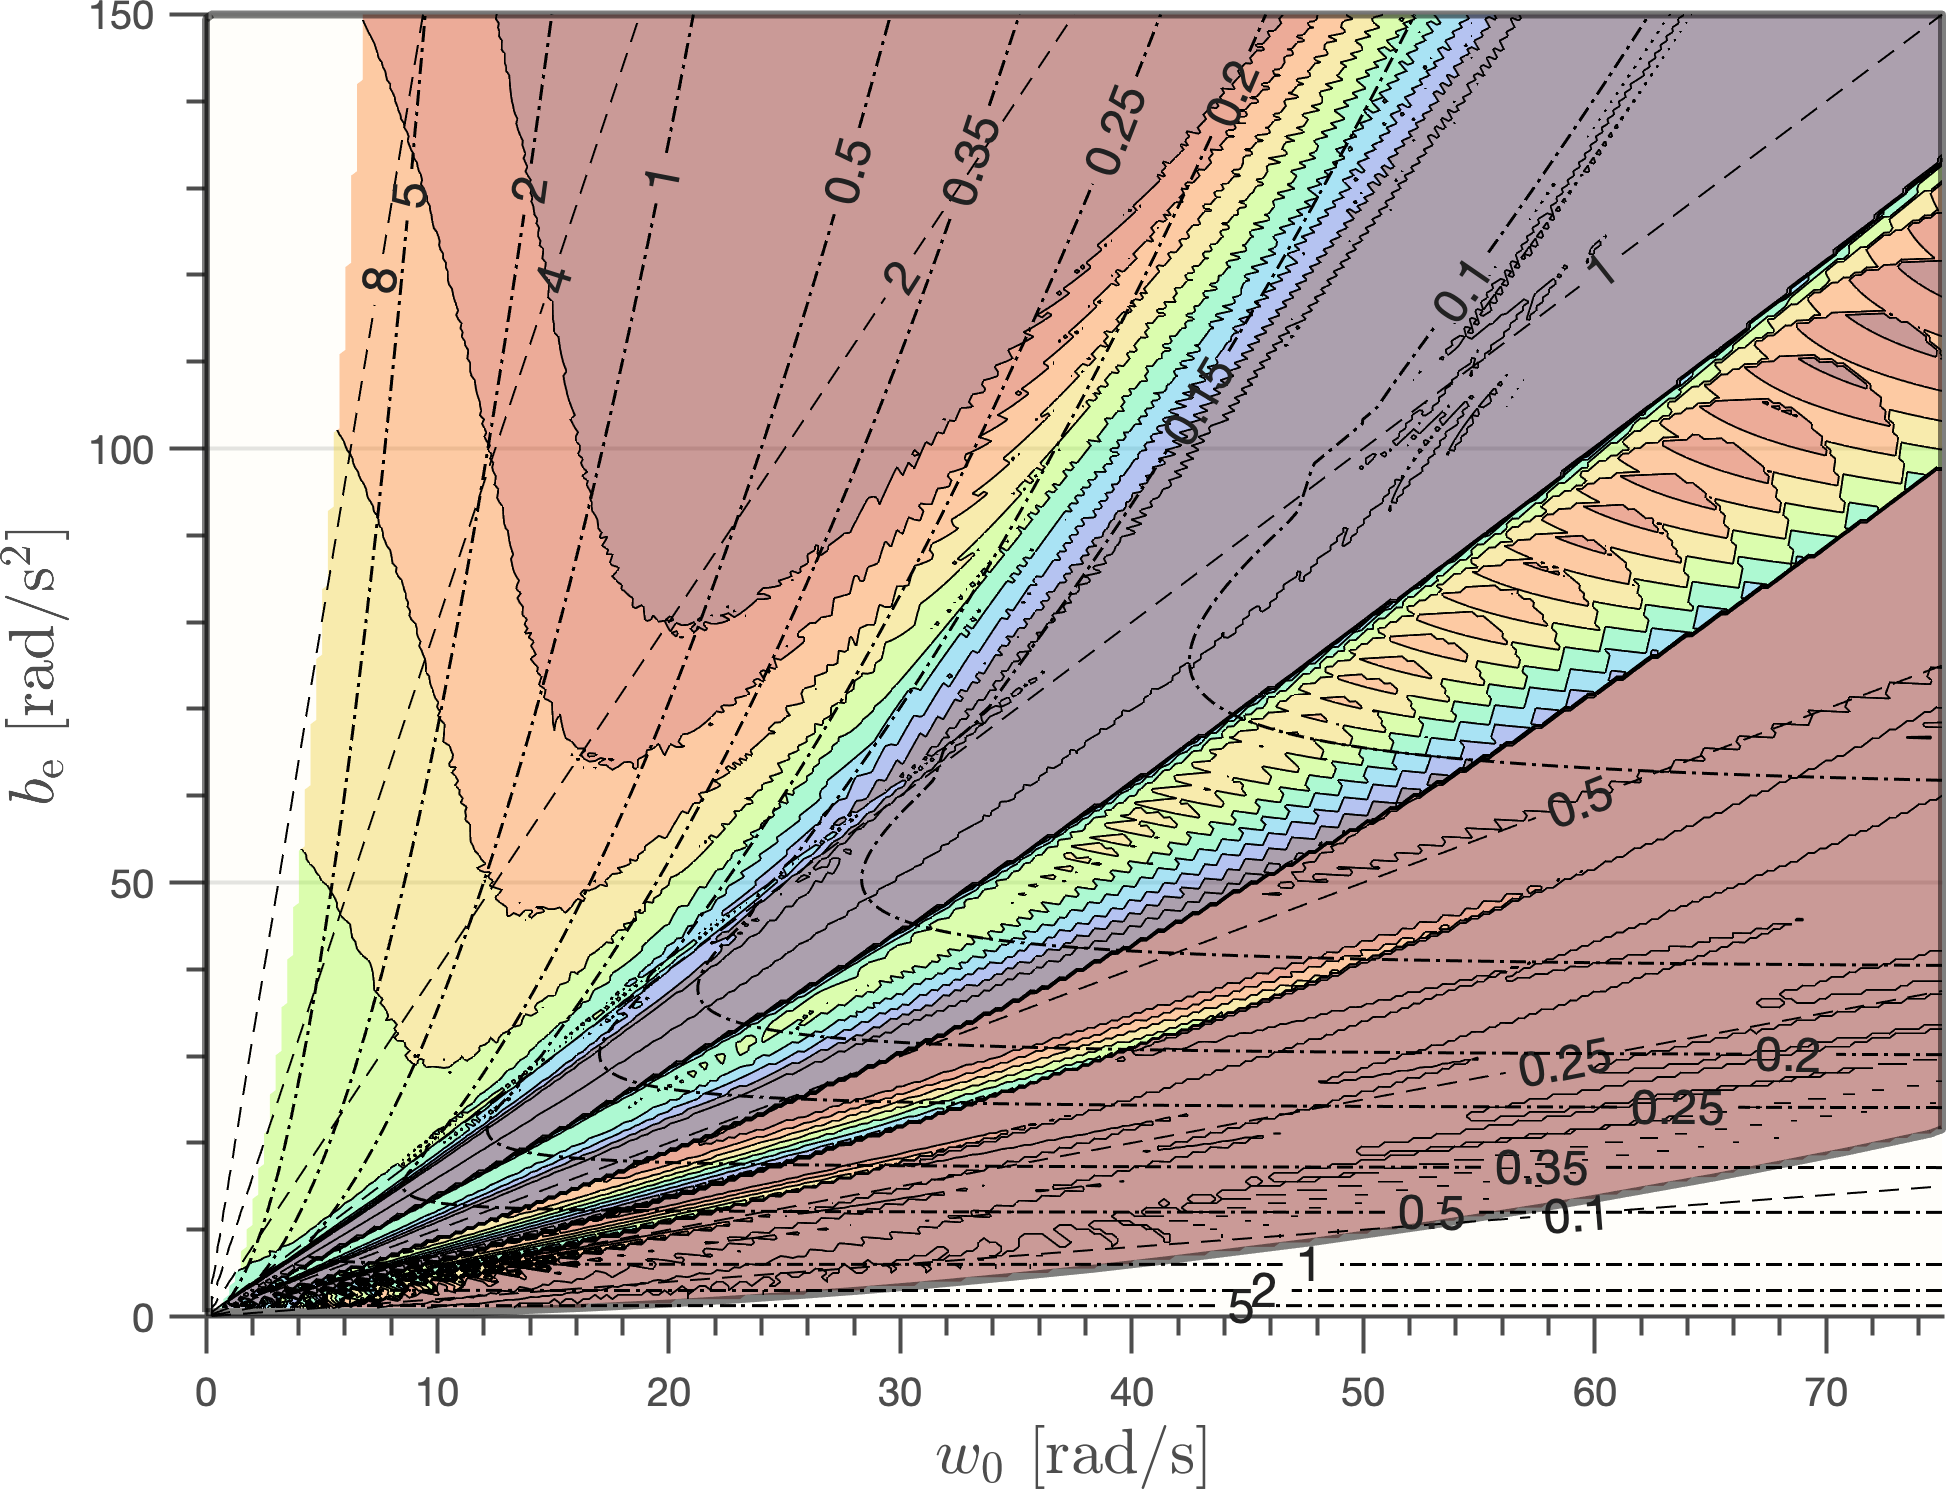
\includegraphics[width=14cm]{images/stab_map_00025.png}
    \caption{Stabilitástérkép 2.5ms időkéséssel}\label{fig:stab_map_00025}
    \end{center}
\end{figure}
\pagebreak
A motorvezérlővel való kommunikáció maximális sebessége és a 10\% relatív hiba alatti terület méretét figyelembe véve 
a végső mérés 5 ms időkéséssel készült. A stabilitástérkép egy egyenletes 50x50-es rács segítségével fel lett 
osztva. Az így kapott 2500 potenciális mérési pont nagy része instabil, vagy a mérés kivitelezhetősége szempontjából 
túl nagy beállási idővel rendelkezik. A tényleges mérési pontok ez alapján a stabil tartományon belül az 1 szekundumnál 
kisebb beállási idővel és a digitális modell predikciója szerint kevesebb, mint 50\% hibával rendelkeznek. Ezen kritériumokkal 
együtt a végleges mérési pontok teljes száma 992 volt. Minden mérési pont meghatároz egy impedancia modell beállítást, mely 
az \ref{fig:measurement_protocol}. ábrán is látható protokoll segítségével automatizált módon került át a szabályozót 
implementáló mikrovezérlőre. Minden mérés ideális esetben 10x lett volna megismételve, azonban ha az adott paraméterek mellett 
nem állt be a rendszer, 10 sikertelen próbálkozás után a következő mérésre ugrott a rendszer. Előfordult olyan köztes eset is, 
amikor részben sikeres, részben sikertelen volt egy adott kísérlet. Ekkor is 10 sorban sikertelen vagy összesen 10 sikeres 
mérés volt a megállási kritérium, viszont legalább 5 sikeres mérés kellett, ahhoz hogy a végső analízisben figyelembe legyen 
véve az adott mérés.
\begin{figure}[H]
    \begin{center}
    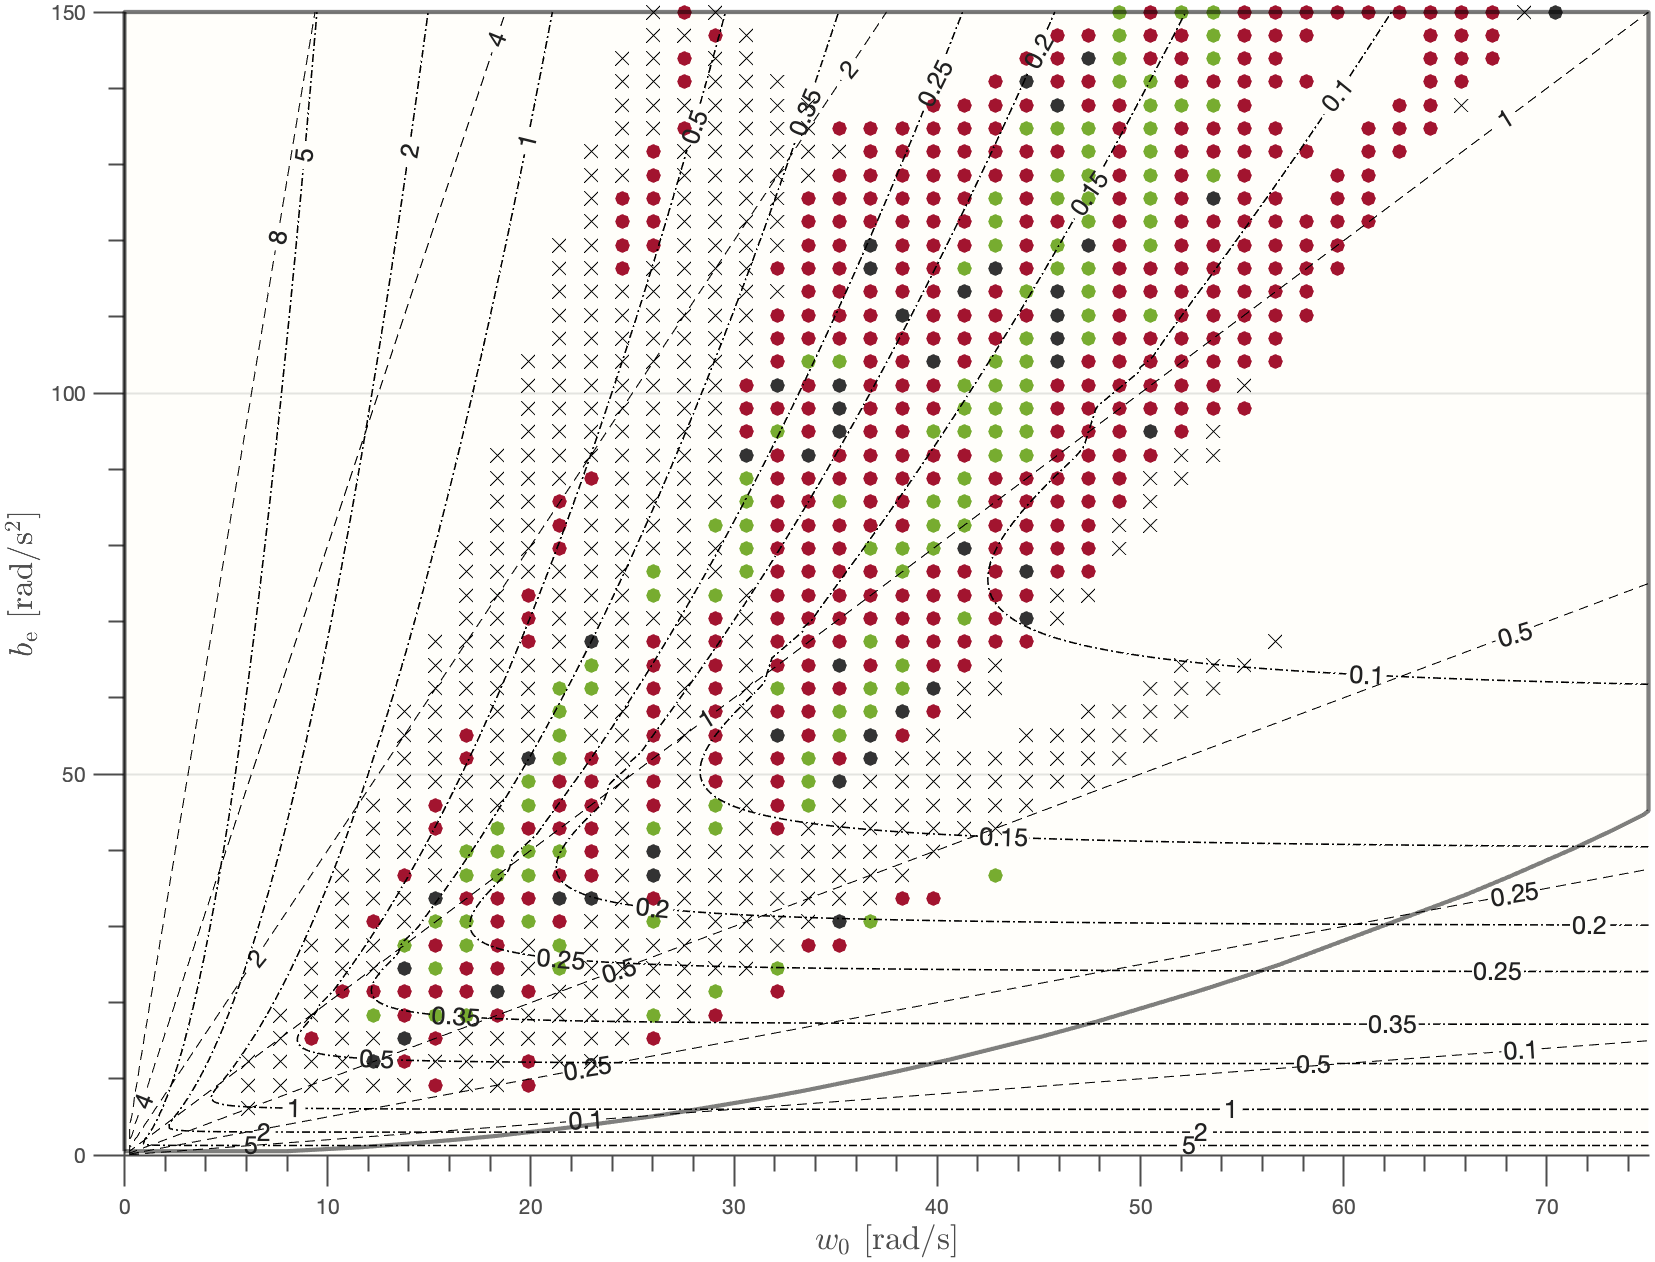
\includegraphics[width=\textwidth]{images/experiment_comparison_0005.png}
    \caption{Mért beállási idők összehasonlítása a modellel 5ms késéssel}\label{fig:experiment_comparison_0005}
    \end{center}
\end{figure}
A teljes futási idő nagyjából 12-15 óra volt. A kapott eredményeket ábrázolja a \ref{fig:experiment_comparison_0005}. ábra.
A pontok közül fekete 'x' jelöli a sikertelennek ítélt méréseket. A többi esetben a mért beállási idők és a digitális 
szabályozóval számolt beállási idők közötti eltérés alapján 7\% szignifikancia mellett irrelevánsnak itélt diszkrepanciát 
jelölik a zöld pontok. 1.2-7\% között indiszkriminánsnak ítélt méréseket jelölik a fekete pontok, és 1.2\%-hoz mérten 
szignifikáns eltérést jelölik a piros pontok. Láthatóan a mérések kevesebb, mint fele felel meg ezeknek a feltételeknek. 
A legtöbb sikeres mérés a stabilitási tartomány azon területén található, ahol a modellezett relatív hiba negatív. Tehát 
a digitális rendszer az elvártnál gyorsabban áll be. 
% A mért beállási időket a függelék \ref{tab:}. táblázata tartalmazza.

\chapter{Összegzés}\label{chap:summary}

A dolgozatban a REHAROB rehabilitációs robot kézmoduljának egyszerűsített modellje került bemutatásra. Egy állandó 
gerjesztésű egyenáramú motorból kiindulva, egy hibrid pozíció-nyomaték szabályozón keresztül, sikerült egy másodrendű 
modell által előírt mozgást rákényszeríteni a rendszerre. A szabályozó egy minimumrendű megfigyelőt 
felhasználva minimalizálja a beépítendő külső szenzorok számát. A beállási idő alapján megalkotott feltétel 
szerint felírható a modell előírt tehetetlensége, viszkózus csillapítási együtthatója és a szabályozó 
pólusai közötti kapcsolat. Az előírt tehetetlenség legfeljebb a fizikai rendszer 2.5-szerese lehet. A minimumát az 
elvárt beállási idő és a szabályozónak beállítható legkisebb pólus határozza meg. 

Az időkéséssel kiegészített modell stabilitását folytonos és diszkrét időben is megvizsgáltam. Mindkét 
esetben elsősorban a modell által előírt viszkózus csillapítási együttható és a rúgóállandó közti 
kapcsolatra adódott új összefüggés. Folytonos esetben elegendően kis időkésésnél lehetséges, hogy tetszőlegesen 
nagy viszkózus csillapítási együttható alkalmazható. Azonban létezik egy kritikus időkésés, ami felett 
a stabilitási tartomány zárt. Ekkor a viszkózus csillapítási együtthatóra is adódik egy maximum. Diszkrét időben csak numerikusan, szimulációkkal sikerült a stabilitási tartományt
meghatározni. A vizsgált paraméterekkel a tartomány mindig zárt volt. A diszkretizált rendszer állapot átmeneti mátrixának 
levezetése után a kapott mátrix sajátértékeinek
vizsgálatával meghatározható a valós és az előírt beállási idő közötti kapcsolat. Ezt is figyelembe véve az 
előírható paraméterkombinációk jóval kisebb tartományban helyezkednek el a teljes stabil területhez képest. Tehát 
az időkésés figyelembevétele nagyban befolyásolja a teljes rendszertervezési folyamatot. Végeredményben jobban 
optimalizálható a motorválasztás és a szabályozót implementáló hardver megtervezése. Költséghatékonyabb és biztonságosabb 
lehet a rendszer, ami egy ember-robot interakciót igénylő alkalmazásban különösen fontos. 


\chapter{Jövőbeli munka}\label{chap:conclusion}

A kapott eredményeket jelen állapotában nem lehet közvetlenül alkalmazni a REHAROB kézmodulján. 
Ehhez a következő lépés, hogy  általánosítsuk a modellt és az eredményeket több szabadsági fokú rendszerekre, ami már megfeleltethető a valódi kézmodulnak. 

A kapott diszkrét idejű stabilitástérképet alaposabban be lehetne járni, 
a motorparaméterek pontosabb meghatározása után. Különböző időkésésekre össze lehetne hasonlítani 
a mért és a szimulált beállási időket. A stabilitás határán ki lehetne mérni a rezgési frekvenciát, 
illetve annak megváltozását a határon végighaladva. 

A beállási időn kívül más rendszerparamétereket 
is meg lehetne vizsgálni, mint a felfutási idő vagy a maximális túllövés. Kiterjeszthető a modell 
nemlineáris hatások bevonásával, ilyen lehetne a Coulomb-súrlódás vagy a szaturáció, esetleg a 
szabályozó jel diszkretizációja. 

A külső nyomaták kompenzációja ugyan bekerült a 
szabályozó modelljébe, de nem maradt idő a kompenzáció tesztelésére. Végül előfordulhat, 
hogy az impedancia modell paramétereit online kell változtatni, például ha ``puhább'' választ 
szeretnénk kapni egy felülettel való kontakt során. Ennek az implementációját és a stabilitásra 
gyakorolt hatását is külön meg kell vizsgálni.


\chapter{Summary}\label{chap:summary_eng}

\begin{otherlanguage}{USenglish}
	\alert{SAME IN ENGLISH}
\end{otherlanguage}


\appendix
\part*{FÜGGELÉK}

% \chapter{A beállási idő analitikus vizsgálata}
% Jól ismert közelítés a beállási időre alulcsillapított rendszereknél a következő formula 
% \begin{equation}
%     t_\RM s = \frac{4}{\zeta \omega_\RM n},
% \end{equation}
% ahol \(\zeta\) a relatív csillapítási hányados és \(\omega_\RM n\) a csillapítatlan 
% sajátkörfrekvencia. Tehát 4 időállandóval becsüli a beállási időt. 
% Ez az összefüggés csak ~2\%-os hibasávra alkalmazható, valamint 
% kritikus csillapítás közelében 30-40\%-al eltér a valódi beállási időtől. Túlcsillapított 
% esetre pedig egyáltalán nem alkalmazható. A legkézenfekvőbb általánosítása a formulának, 
% ha az időállandót a domináns pólussal helyettesítjük. Ez túlcsillapított esetre is ad 
% egy megoldást, de kritikus csillapítás közelében továbbra is nagy eltérést eredményez.
% Túlcsillapított esetre a domináns pólussal a formula a következő
% \begin{equation}
%     t_\RM s = \frac{4}{\left(\zeta-\sqrt{\zeta^2-1}\right) \omega_\RM n}.
% \end{equation}
% A stabilitásvizsgálat során olyan formulák kellettek, amelyek a kritikus csillapítás 
% közelében is relatíve kis hibával bírnak. Ehhez előszőr is szükség lesz a másodrendű 
% rendszer általános megoldására időtartományban egységugrás bemenetre valamint \(x_0\)
% kezdeti elmozdulásra és zérus kezdeti sebességre. Ez számtalan módon 
% megkapható. Az eredmény a következő 
% \begin{equation}
%     x(t) = x_0 e^{-\zeta\omega_\RM n t}\left[
%         \frac{1}{2}\left(e^{i\omega_\RM d t} + e^{-i\omega_\RM d t}\right)
%         - \frac{\zeta}{\sqrt{\zeta^2-1}}\frac{1}{2}\left(e^{i\omega_\RM d t} - e^{-i\omega_\RM d t}\right)
%         \right],
% \end{equation}
% ahol \(\omega_\RM d\) a csillapított sajátkörfrekvencia
% \begin{equation}
%     \omega_\RM d = \sqrt{1-\zeta^2}\omega_\RM n.
% \end{equation}
% Kritikus csillapítás közelében a válaszfüggvény a következő alakra hozható \(e^{ix}\) 
% hátványsorba fejtett alakjával 
% \begin{equation}
%     x(t) = x_0 e^{-\zeta\omega_\RM n t}\left(1 + \omega_\RM n t\right).
% \end{equation}
% Legyen a hibasáv mérete a kezdeti és a végérték közötti távolsággal arányosan kifejezve \(\Delta\).
% Felhasználva hogy a válasz szigorúan monoton, a beállási idő elteltével a következő összefüggés 
% lesz érvényben
% \begin{equation}
%     \Delta x_0 = x_0 e^{-\zeta\omega_\RM n t_\RM s}\left(1 + \omega_\RM n t_\RM s\right).
% \end{equation}
% Ez az egyenlet a Lambert-féle W-függvény segítségével kifejezhető a beállási időre
% \begin{equation}
%     t_\RM s = -\frac{W_{-1}(-\frac{\Delta}{e})+1}{\omega_n},
% \end{equation}
% ahol \(W_{-1}(x)\) a Lambert-féle W-függvény \(W \le -1\)-ra értelmezett ága és \(\Delta\) a 
% \([0, 1]\) intervallumon belül található. Például 2\%-os hibasáv esetén kritikus csillapításnál 
% \begin{equation}
% t_\RM s = \frac{5.8339}{\omega_n}.
% \end{equation}
% Ez körülbelül 30\%-al eltér a négy időállandós becsléstől. \(\zeta=1\) közelében 
% nem sikerült Taylor-sorral általánosítani a formulát, de empirikusan egy jó közelítésnek 
% bizonyult egy lineáris taggal kiegészíteni az előző összefüggést
% \begin{equation}
% t_\RM s = -\frac{W_{-1}(-\frac{\Delta}{e})+1}{\omega_n} + \frac{15}{\omega_\RM n}\left(\zeta-1\right),
% \end{equation}
% mely \(0.98 \le \zeta \le 1.03\) tartományban alkalmazható.


\chapter{A PWM frekvencia hatása DC motor vezérlésénél}\label{chap:effects_of_pwm_frequency}
A mérési összeállítás tervezése során először egy jóval alacsonyabb PWM frekvenciával működő 
motorvezélő lett bekötve. A motor állandósult sebessége és a PWM jel kitöltési tényezője közötti kapcsolat 
erősen nemlineáris volt az első tesztek során. Ennek a VNH5019 alapú Polulu motorvezérlőnek a kimeneti frekvenciája 
maximum 20 kHz volt. Egy ilyen előzetes mérés eredménye látható az \ref{fig:motor_response_20khz}. ábrán. 

\begin{figure}[b!]
    \begin{center}
    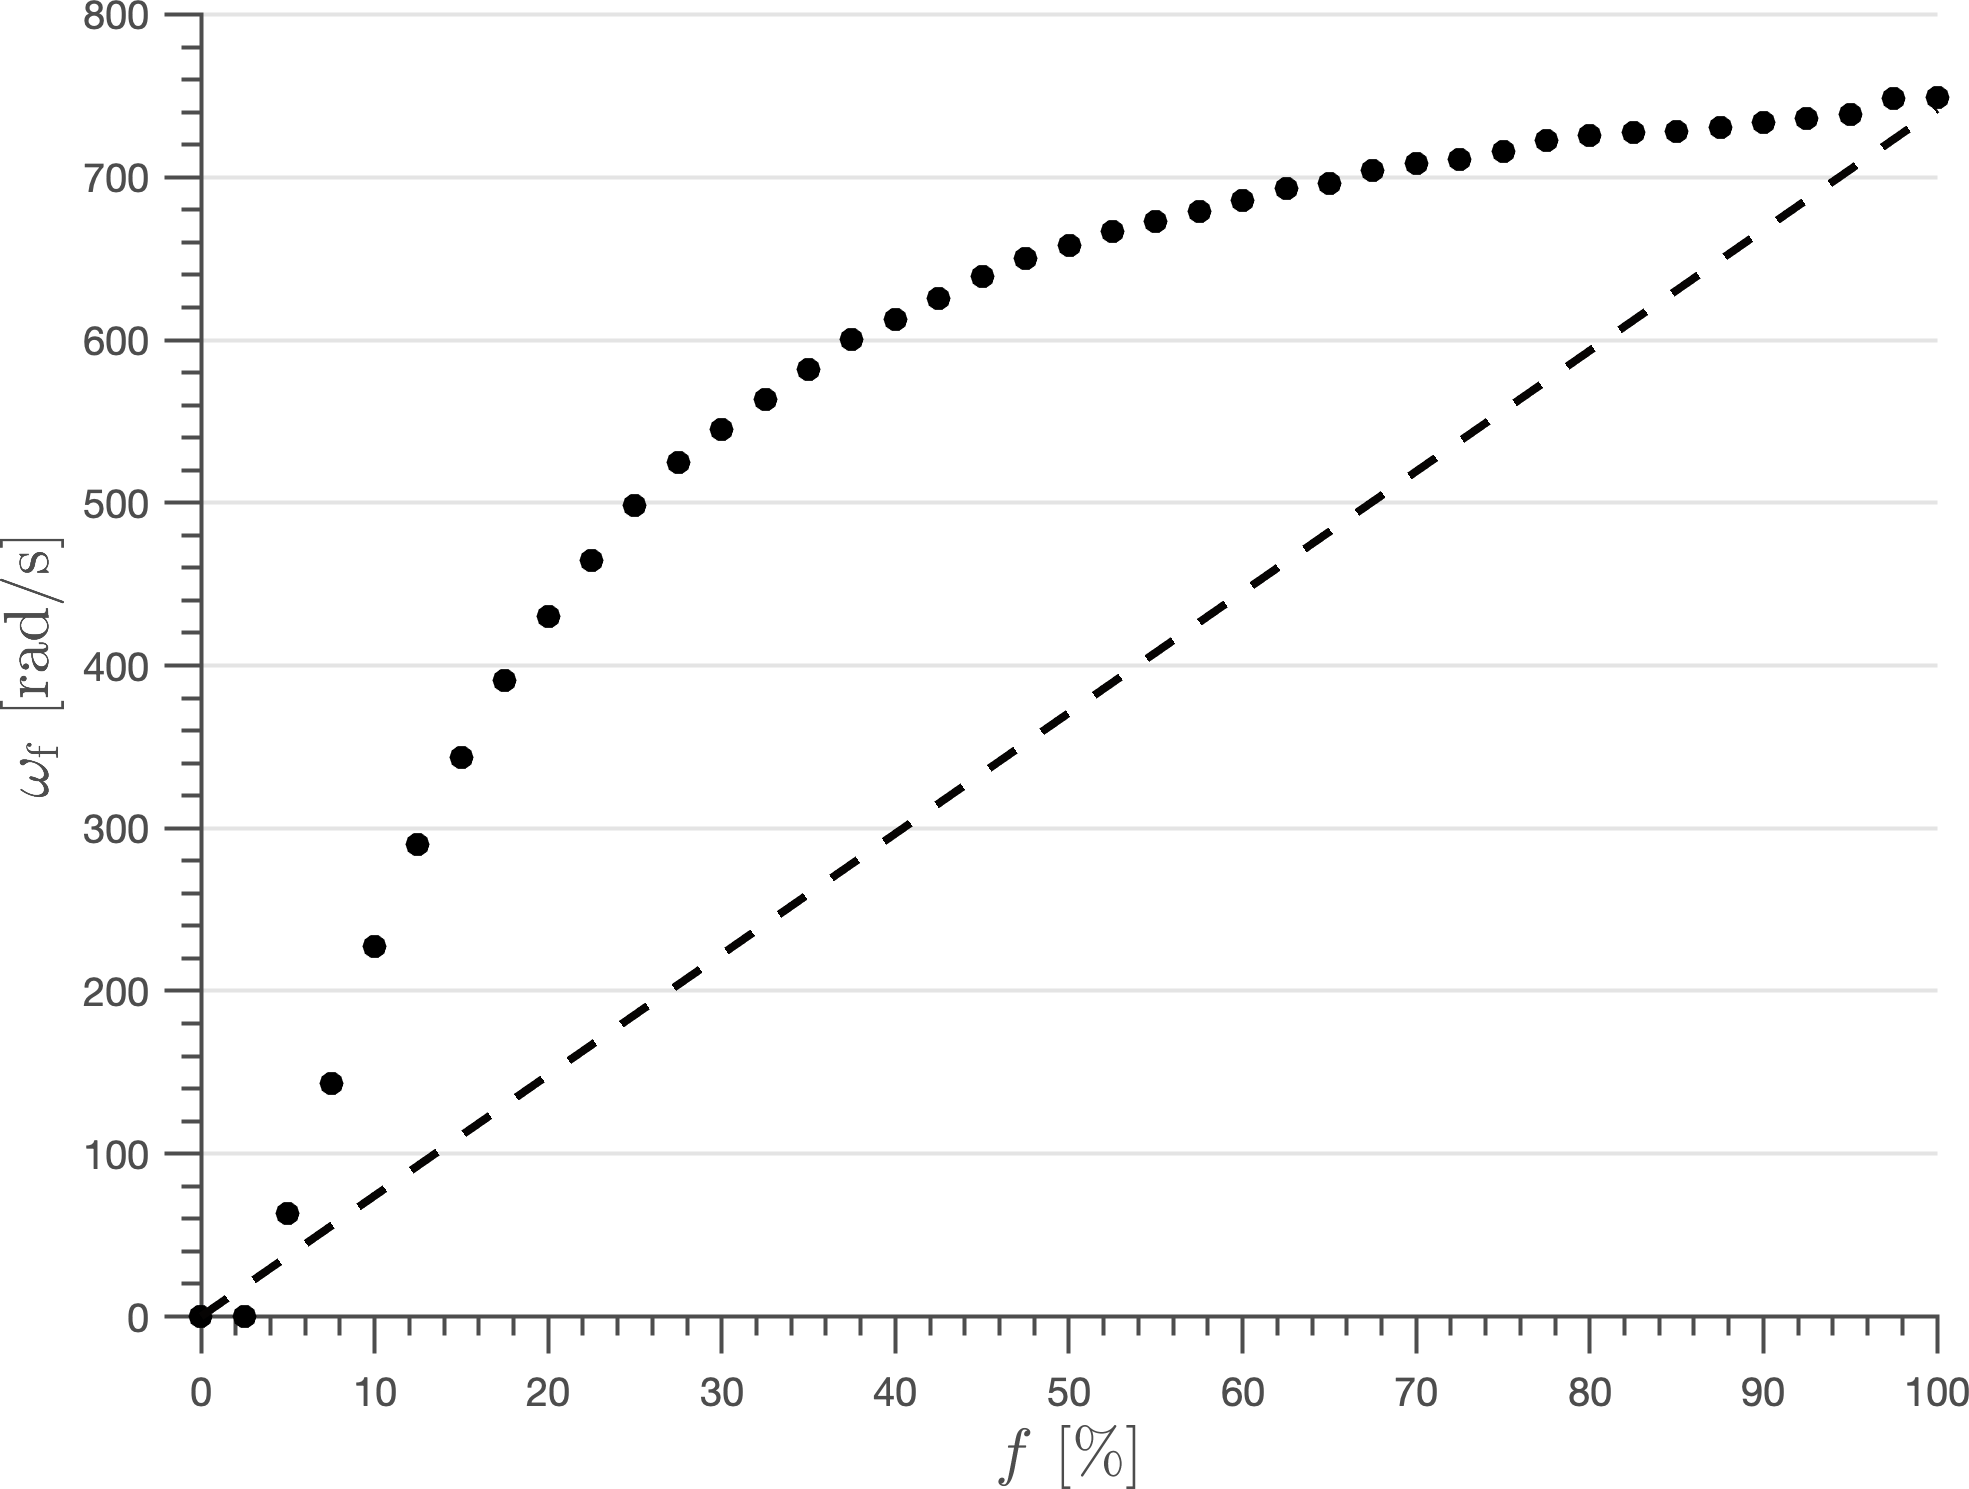
\includegraphics[width=14cm]{images/motor_pwm_response20.png}
    \caption{A motor állandósult sebessége és a kitöltési tényező viszonya 20 kHz-es PWM jellel.}\label{fig:motor_response_20khz}
    \end{center}
\end{figure}

Az \ref{fig:speed_profile}. ábrával ellentétben a maximális sebesség nagyobb volt, mivel a 
terhelésként használt propeller ekkor még nem került a motorra. A szabályozó tervezése során alapfeltevés volt, hogy 
a motorra kapcsolt feszültség változatlan marad, ha a szabályozó kimenete állandó. Láthatóan a motor máshogy viselkedik 
a PWM jel hatására, mintha a PWM jel átlagfeszültségével megegyező nagyságú állandó feszültség lenne a motorra kapcsolva.
Ennek a jelenségnek a magyarázatához elég a \ref{chap:physical_system}. fejezetben bevezetett lineáris modell válaszát 
megvizsgálni PWM bemenetre. A PWM jel két részre bontható. Az első szakasz változtatható szélességű és a 
kimeneti feszültség maximum, a második szakaszban a kimeneti feszültség zérus 
\begin{equation}
    V(t) = 
    \begin{cases}
        V_\RM{max} & \text{ha } kt_\RM p \le t < ft_\RM p + kt_\RM p \\
        0 & \text{ha } ft_\RM p + kt_\RM p \le t < (k+1)t_\RM p
    \end{cases}\,,
\end{equation}
ahol \(t_\RM p\) a jel periódusideje és \(f\) a kitöltési tényező.
A rotor áramának dinamikáját az \eqref{eq:armature_circuit} egyenlet írja le. 
Állandó feszültségre megoldva az idő és az áram szeparálásával
\begin{equation}
    \begin{split}
    \int_{t_0}^{t} dt &= \int_{i_0}^{i} \frac{L di}{V-K_\RM m\dot\theta - Ri}, \\
    t - t_0 &= -\frac{L}{R} \ln \frac{V-K_\RM m\dot\theta-Ri}{V-K_\RM m\dot\theta-Ri_0}, \\
    i(t) &= \frac{V-K_\RM m\dot\theta}{R}\left(1-e^{-\frac{t-t_0}{L/R}} \right) + i_0 e^{-\frac{t-t_0}{L/R}}. 
    \end{split}
\end{equation}
A megoldás során alkalmazott feltételezés, hogy a rotor forgási sebessége állandónak tekinthető állandósult esetben. 
Ez egy realisztikus feltételezés, hiszen a motor mechanikai időállandója nagyságrendekkel nagyobb a PWM jel periódusidejénél 
a vizsgált rendszerben. Ugyanebből a feltételezésből következik, hogy elég a motorra ható forgatónyomaték átlagát figyelembe venni, 
mely~\eqref{eq:lenz_torque} alapján arányos a tekercsárammal. Az átlag meghatározásához két esetet kell figyelembe venni. 
Az első esetben a tekercsáram nulláról indul és még kevesebb mint egy periódus alatt visszaesik nullára. Ez a továbbiakban szakaszos üzemmódnak 
lesz hívva. A másik eset, hogy a kiinduláskor nullától eltérő tekercsáram pontosan a periódus végén esik vissza a kiindulási értékére. 
Ez lesz a folytonos üzemmód. Az átlag meghatározásához fel lett használva az a feltételezés, hogy elegendő az előbb kapott 
exponenciális változást leíró formula lineáris közelítését felhasználni. A közelítés szerint 
\begin{equation}
    \begin{split}
        i(t) &= (i_\RM{max} - i_0)\frac{t}{ft_\RM p} + i_0, \\
        i_\RM{max} &= \frac{V-K_\RM m\dot\theta}{R}\left(1-e^{-\frac{ft_\RM p}{L/R}} \right) + i_0 e^{-\frac{ft_\RM p}{L/R}}
    \end{split}
\end{equation}
amíg a feszültség értéke maximum. Szakaszos üzemmódban meg kell határozni az áram nullára visszaeséséhez szükséges időt. 
Ez az előző egyenletek alapján 
\begin{equation}
    t_f = \frac{L}{R}\ln\left[\frac{V}{K_\RM m\dot\theta}\left(e^{-\frac{ft_\RM p}{L/R}} - 1\right) + 1\right]
\end{equation}
a periódus kezdetéhez viszonyítva.
A tekercsáram átlaga ez alapján belátható hogy a következő összefüggéssel közelíthető
\begin{equation}
    \begin{split}
    i_\RM{avg} &= \frac{1}{2}i_\RM{max}\frac{t_\RM f}{t_\RM p} \\
               &= \frac{1}{2}\frac{V-K_\RM m\dot\theta}{R}\left(1-e^{-\frac{ft_\RM p}{L/R}} \right)\frac{L}{t_\RM p R}\ln\left[\frac{V}{K_\RM m\dot\theta}\left(e^{-\frac{ft_\RM p}{L/R}} - 1\right) + 1\right].
    \end{split}
\end{equation}
Folytonos üzemmódban a kezdeti tekercsáramot kell meghatározni felhasználva, hogy \(t_\RM f = t_\RM p\).
Az előző formulák alapján 
\begin{equation}
    i_0 = \frac{V}{R}\frac{1-e^{\frac{ft_\RM p}{L/R}}}{1-e^{\frac{t_\RM p}{L/R}}} - \frac{K_\RM m\dot\theta}{R}.
\end{equation}
Ebben az esetben a tekercsáram átlaga pedig
\begin{equation}
    \begin{split}
    i_\RM{avg} &= \frac{1}{2}\left(i_\RM{max}-i_0\right) + i_0 \\
               &= \frac{1}{2}\left[\frac{V-K_\RM m\dot\theta}{R}\left(1-e^{-\frac{ft_\RM p}{L/R}} \right) + 
               \left(1+e^{-\frac{ft_\RM p}{L/R}} \right)
               \left(\frac{V}{R}\frac{1-e^{\frac{ft_\RM p}{L/R}}}{1-e^{\frac{t_\RM p}{L/R}}} - \frac{K_\RM m\dot\theta}{R}\right)\right].
    \end{split}
\end{equation}
A tekercsáram mindvégig pozitív marad, így kifejezhető a motor szögsebessége és a kitöltési tényező közötti 
kapcsolat folytonos üzemmódban 
\begin{equation}
    \dot\theta_\RM{crit} \le \frac{V}{K_\RM m}\frac{1-e^{\frac{ft_\RM p}{L/R}}}{1-e^{\frac{t_\RM p}{L/R}}}.
\end{equation}
Az átlag áramot behelyettesítve az \eqref{eq:rotor_dynamics} egyenletbe állandósult állapotban 
\begin{equation}
    B_\RM m\dot\theta = K_\RM m i_\RM{avg} + \tau_\RM e,
\end{equation}
ahol \(\tau_\RM e\) itt a statikus súrlódást fogja modellezni. Láthatóan létezik egy minimum kitöltési tényező 
ami alatt el sem indul a motor. 
Az \ref{fig:motor_response_20khz_with_model}. ábrán látható a 20kHz-en mért válasz és a modell által megjósolt viselkedés. 
A szaggatott görbe a kritikus szögsebességet jelöli, amely alatt folytonos üzemmódba lép át a rendszer. Felette pedig szakaszos üzemmódban működik. 

\begin{figure}[t!]
    \begin{center}
    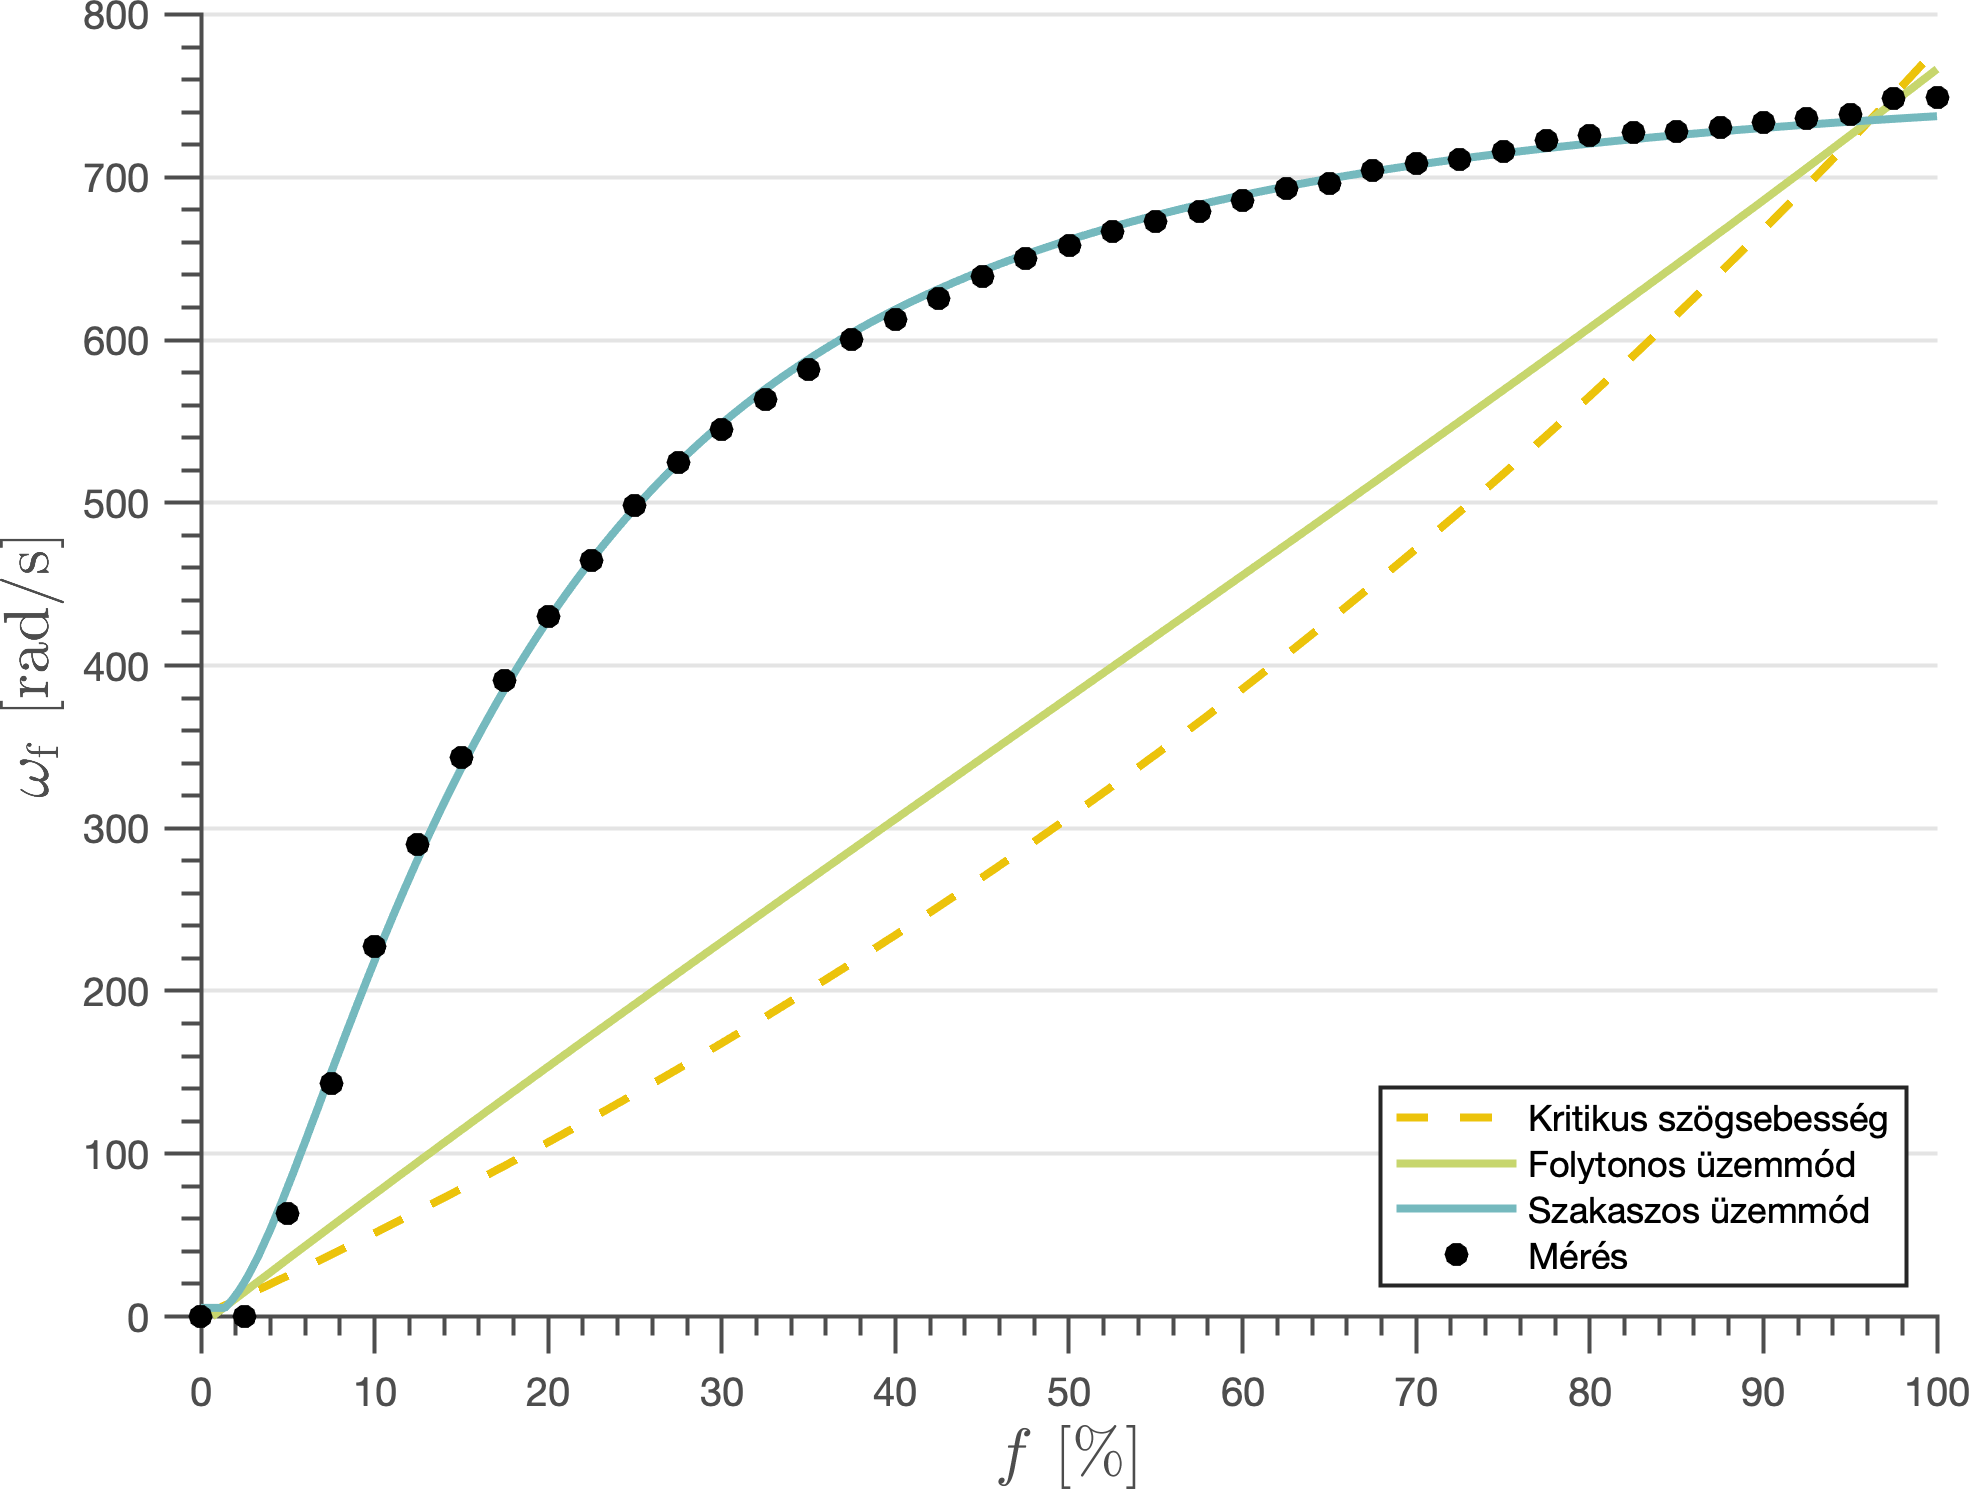
\includegraphics[width=\textwidth]{images/motor_pwm_response20_with_model.png}
    \caption{A motor állandósult sebessége és a kitöltési tényező viszonya modellekkel kiegészítve, 20 kHz-es PWM jellel.}\label{fig:motor_response_20khz_with_model}
    \end{center}
\end{figure}

A statikus súrlódásból származó nyomatékra \(\tau_\RM e = 1.5 \times 10^{-4}~\RM{Nm}\), a viszkózus csillapítási együtthatóra pedig 
\(B_\RM m = 2.7 \times 10^{-7}~\RM{kg \cdot m^2 \cdot s^{-1}}\) lett behelyettesítve. A többi paraméter az adatlapból származik. 
A mérés külső terhelés vagy hozzáadott tehetetlenség nélkül történt. Az egyezés jól látható, és az is látszik, hogy majdnem a 
teljes tartományon szakaszos üzemmódban működik a rendszer. A folytonos üzemmód viszont teljesen elfogadható 
lineáris viszonyt adna. A frekvencia és a viszkózus csillapítás növelésével el lehet érni, hogy a rendszer majdnem teljes 
egészében folytonos üzemmódban operáljon. A maxon ajánlása egyébként legalább 50 kHz használata a saját motorjaiknál, 
de ehhez nem adnak bővebb indoklást. Egy másik lehetőség a tekercs induktivitásának megnövelése például egy sorba kötött kis 
induktivitású folytótekerccsel. Ennek a módszernek viszont jóval kisebb hatása van a linearitásra a frekvenciához vagy a 
viszkeozus csillapítási együtthatóhoz képest. Még érdekesebb módszer lehet a súrlódás megnövelése. Ez ugyanúgy linearizálja a rendszert. 
Lehetnek alkalmazások, ahol ez az optimális megoldás. 

\chapter{Adatlapok}
\begin{figure}[H]
    \begin{center}
    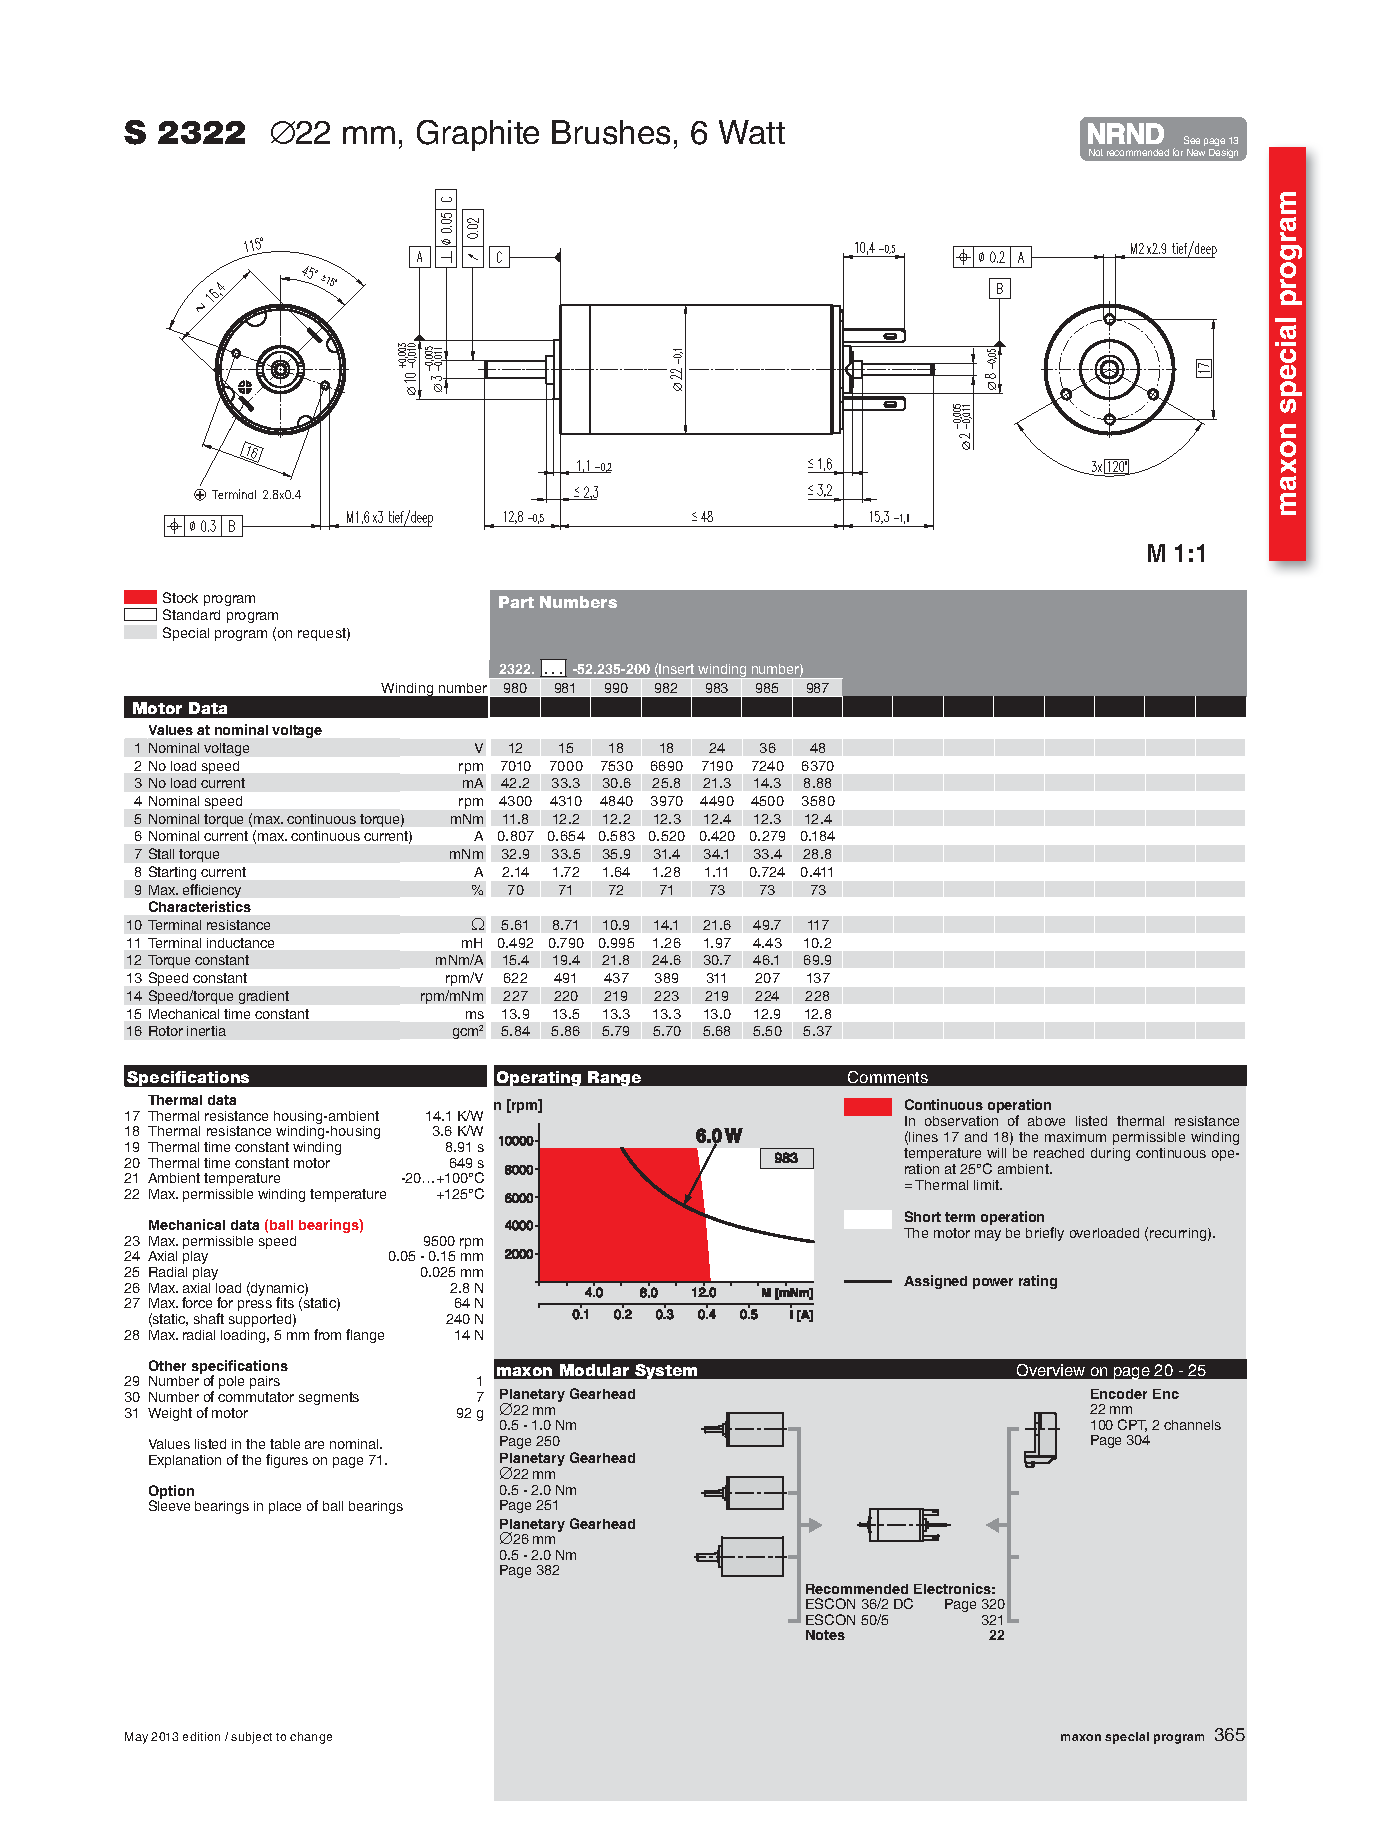
\includegraphics[width=\textwidth]{images/motor.pdf}
    \caption{Motor adatlap}\label{fig:motor_datasheet}
    \end{center}
\end{figure}

\begin{figure}[H]
    \begin{center}
    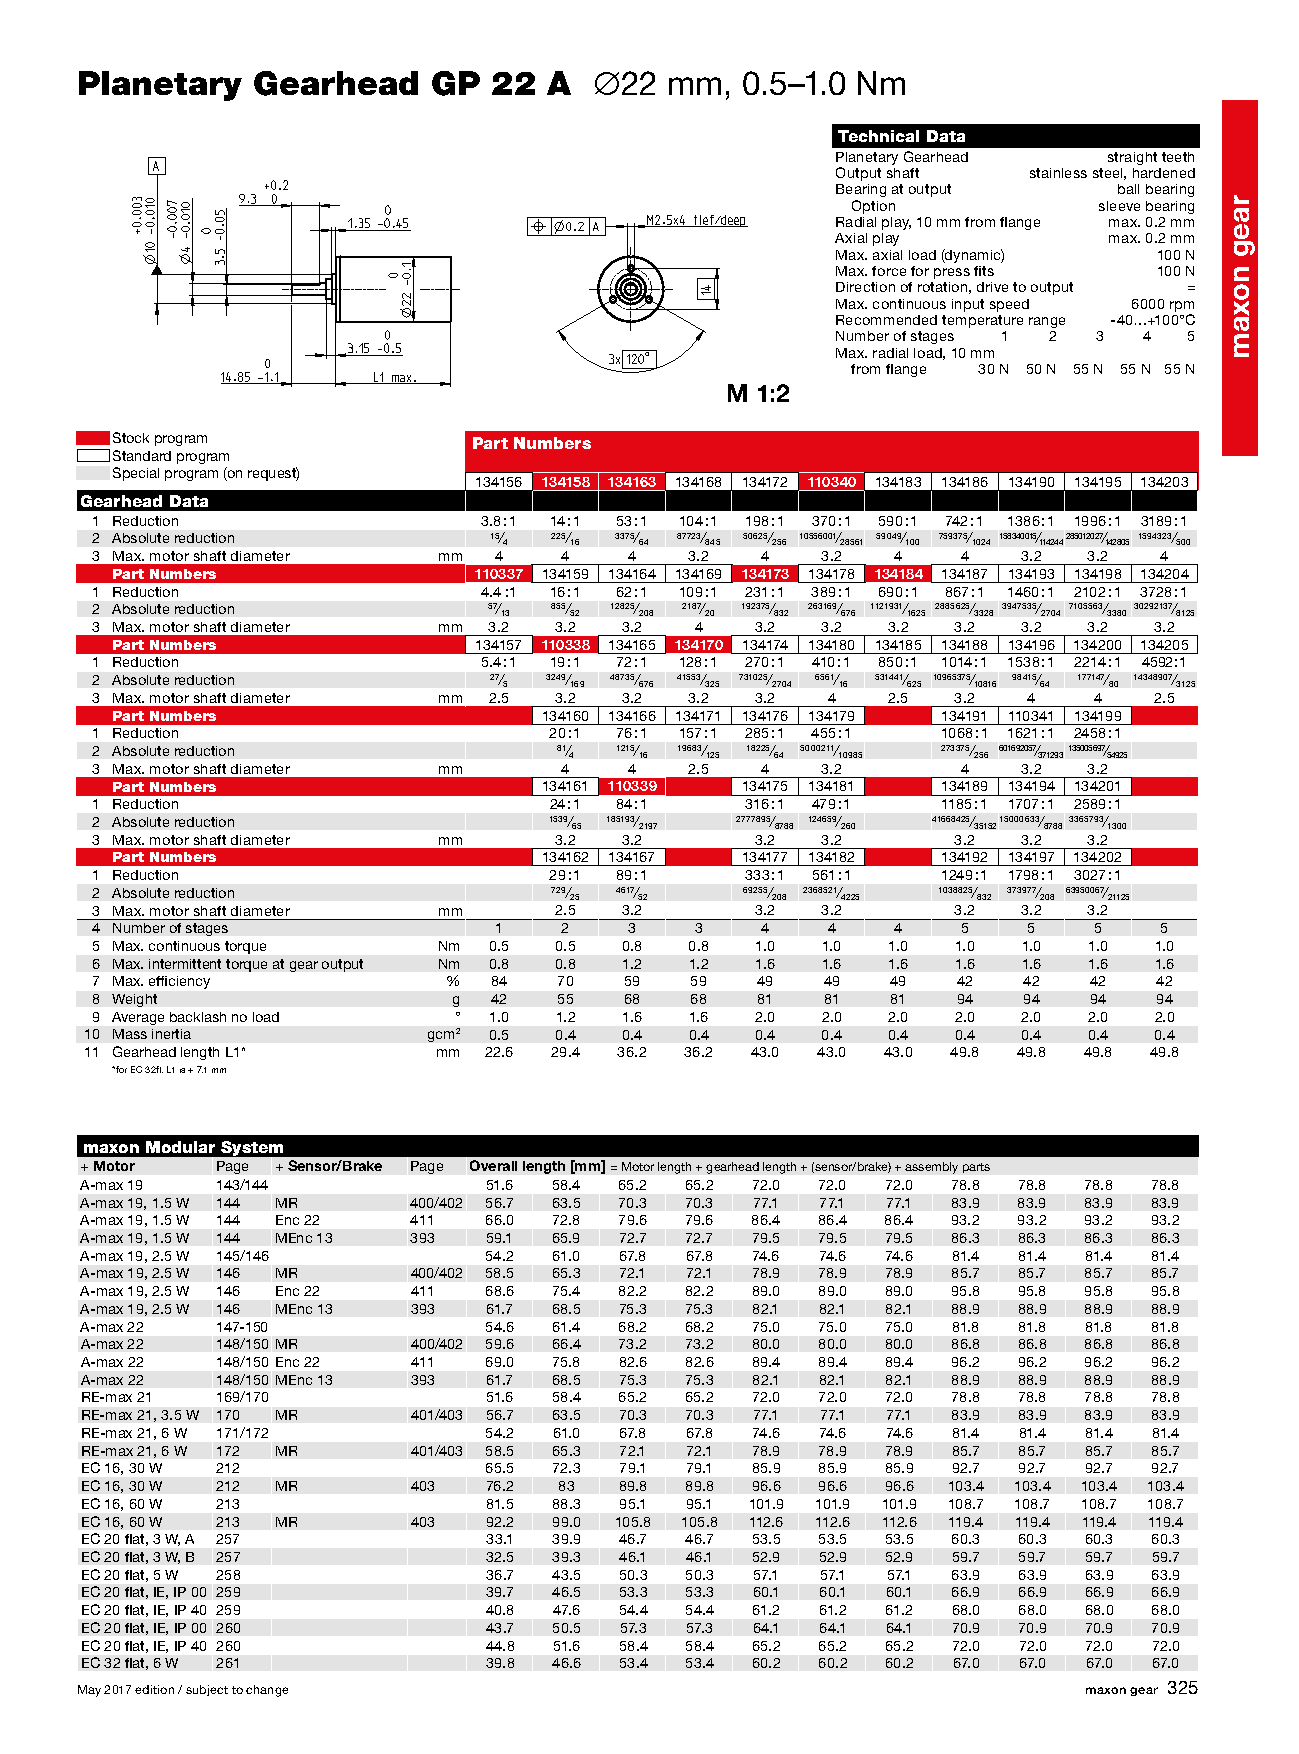
\includegraphics[width=\textwidth]{images/gearhead.pdf}
    \caption{Hajtómű adatlap}\label{fig:gearhead_datasheet}
    \end{center}
\end{figure}

\begin{figure}[H]
    \begin{center}
    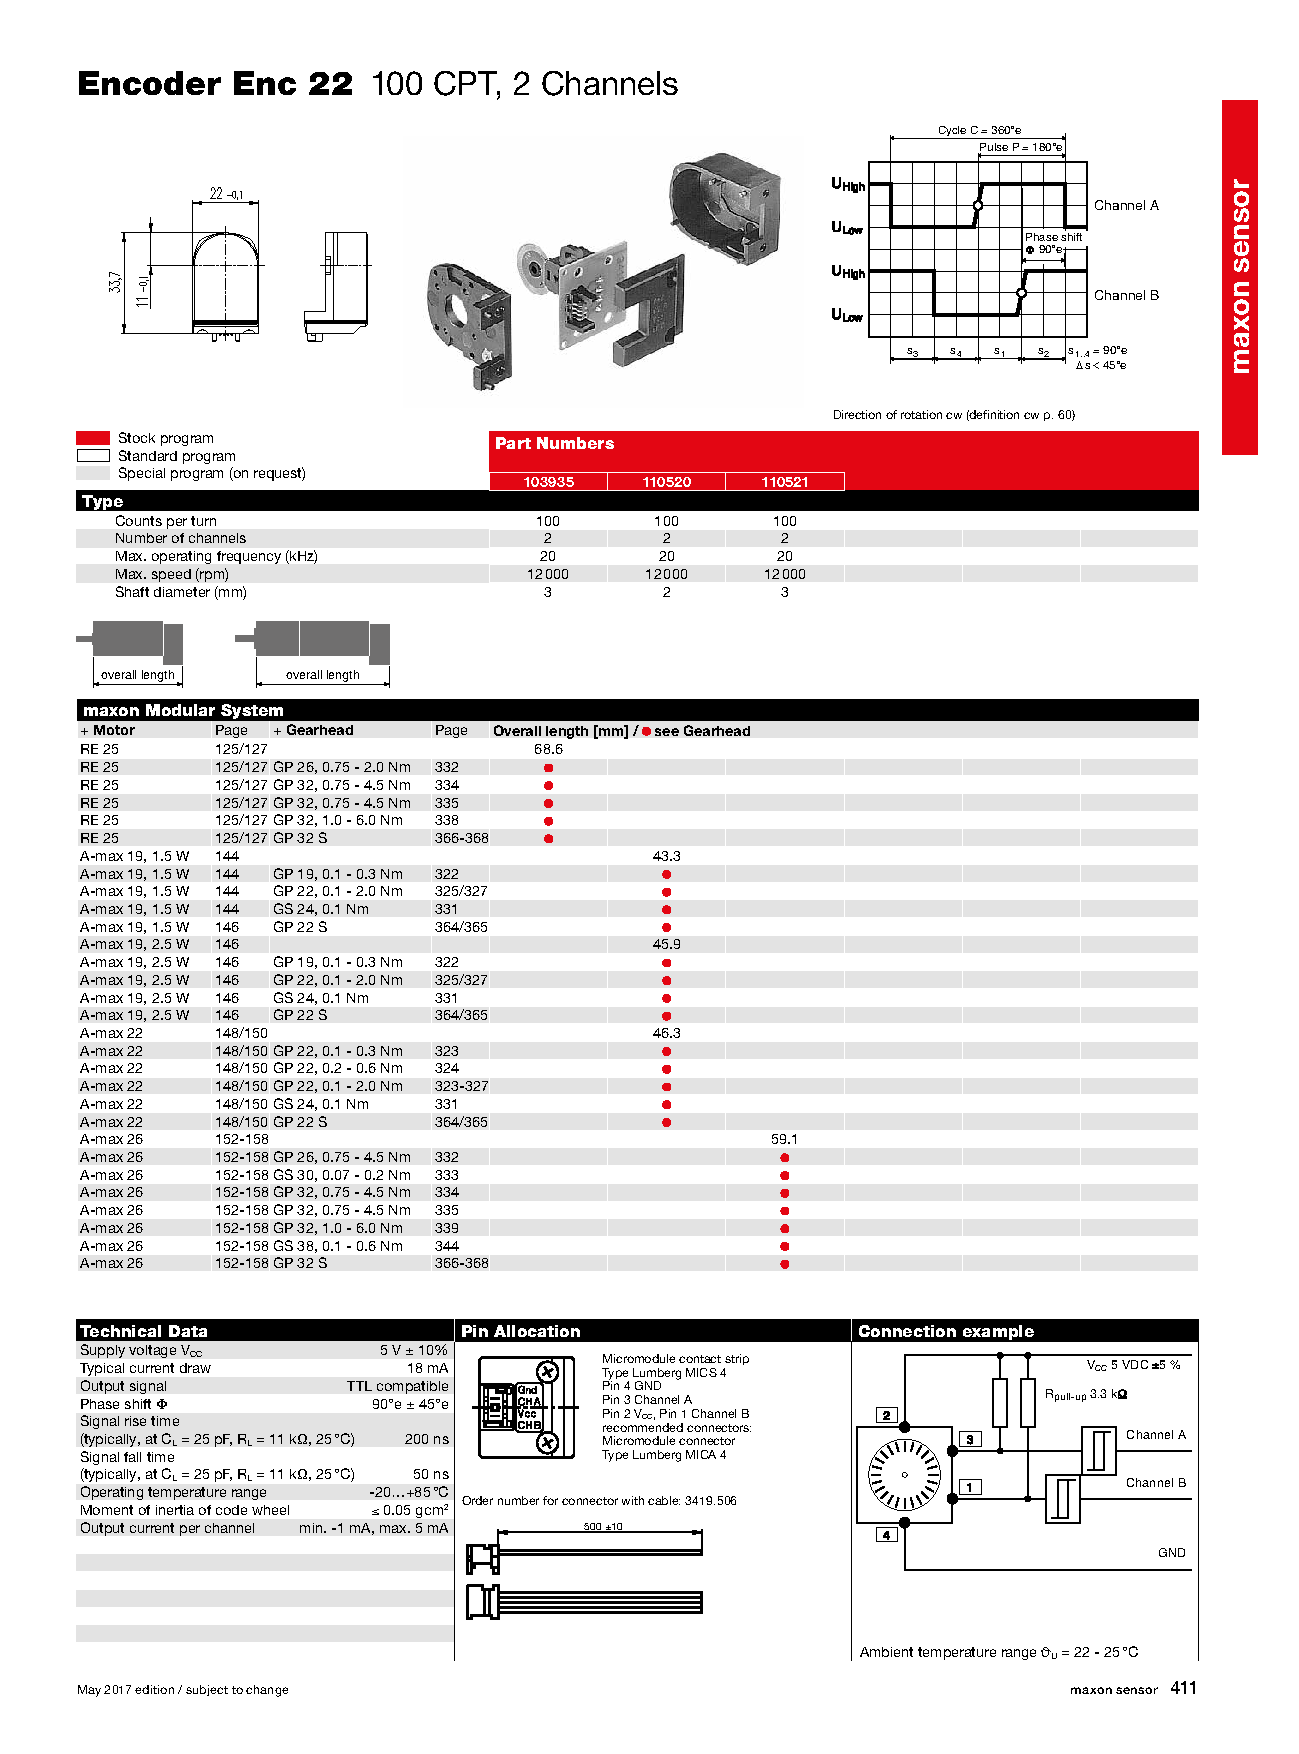
\includegraphics[width=\textwidth]{images/encoder.pdf}
    \caption{Enkóder adatlap}\label{fig:encoder_datasheet}
    \end{center}
\end{figure}

% \begin{table}[H]
%     \small\centering
%     \caption{Motor végsebesség és kapocsfeszültség mérések}\label{tab:speed_profile}
%     \tabcolsep=2pt
%     \begin{tabular}{d{-1}>{~}d{-1}>{~}d{-1}>{~}d{-1}}
%         \toprule
%         \multicolumn{1}{c}{Sajátkörfrekvencia [rad/s]} & \multicolumn{1}{c}{ []} & \multicolumn{1}{c}{ []} & \multicolumn{1}{c}{Hiba [ms]} \\ 
%         \multicolumn{1}{c}{\(\omega_\RM 0\)} & \multicolumn{1}{c}{\(b_\RM e\)} & \multicolumn{1}{c}{\(t_\RM s\)} & \multicolumn{1}{c}{\(\delta t_\RM s\)} \\
%         \midrule
%         6.12 & 6.12 & - & - \\
%         6.12 & 9.18 & - & - \\
%         6.12 & 12.24 & - & - \\
%         7.65 & 9.18 & - & - \\
%         7.65 & 12.24 & - & - \\
%         7.65 & 15.31 & - & - \\
%         7.65 & 18.37 & - & - \\
%         9.18 & 9.18 & - & - \\
%         9.18 & 12.24 & - & - \\
%         9.18 & 15.31 & 500 & 10 \\
%         9.18 & 18.37 & - & - \\
%         9.18 & 21.43 & - & - \\
%         9.18 & 24.49 & - & - \\
%         9.18 & 27.55 & - & - \\
%         10.71 & 9.18 & - & - \\
%         10.71 & 12.24 & - & - \\
%         10.71 & 15.31 & - & - \\
%         10.71 & 18.37 & - & - \\
%         10.71 & 21.43 & 415 & 4 \\
%         10.71 & 24.49 & - & - \\
%         10.71 & 27.55 & - & - \\
%         10.71 & 30.61 & - & - \\
%         10.71 & 33.67 & - & - \\
%         10.71 & 36.73 & - & - \\
%         12.24 & 9.18 & - & - \\
%         12.24 & 12.24 & 540 & 70 \\
%         12.24 & 15.31 & - & - \\
%         12.24 & 18.37 & 232 & 2 \\
%         12.24 & 21.43 & 460 & 40 \\
%         12.24 & 24.49 & - & - \\
%         12.24 & 27.55 & - & - \\
%         12.24 & 30.61 & 439 & 6 \\
%         12.24 & 33.67 & - & - \\
%         12.24 & 36.73 & - & - \\
%         12.24 & 39.80 & - & - \\
%         12.24 & 42.86 & - & - \\
%         12.24 & 45.92 & - & - \\
%         13.78 & 9.18 & - & - \\
%         13.78 & 12.24 & 363 & 2 \\
%         13.78 & 15.31 & 396 & 9 \\
%         13.78 & 18.37 & 280 & 20 \\
%         13.78 & 21.43 & 217.6 & 0.5 \\
%         13.78 & 24.49 & 257 & 1 \\
%         13.78 & 27.55 & 370 & 40 \\
%         13.78 & 30.61 & - & - \\
%         13.78 & 33.67 & - & - \\
%         13.78 & 36.73 & 370 & 10 \\
%         13.78 & 39.80 & - & - \\
%         13.78 & 42.86 & - & - \\
%         13.78 & 45.92 & - & - \\
%         13.78 & 48.98 & - & - \\
%         13.78 & 52.04 & - & - \\
%         13.78 & 55.10 & - & - \\
%         13.78 & 58.16 & - & - \\
%         15.31 & 9.18 & 545 & 3 \\
%         15.31 & 12.24 & - & - \\
%         15.31 & 15.31 & 325 & 3 \\
%         15.31 & 18.37 & 337 & 9 \\
%         15.31 & 21.43 & 170.8 & 0.5 \\
%         15.31 & 24.49 & 210 & 10 \\
%         15.31 & 27.55 & 230.1 & 0.8 \\
%         15.31 & 30.61 & 280 & 30 \\
%         15.31 & 33.67 & 430 & 30 \\
%         15.31 & 36.73 & - & - \\
%         15.31 & 39.80 & - & - \\
%         15.31 & 42.86 & 326 & 2 \\
%         15.31 & 45.92 & 372 & 7 \\
%         15.31 & 48.98 & - & - \\
%         15.31 & 52.04 & - & - \\
%         15.31 & 55.10 & - & - \\
%         15.31 & 58.16 & - & - \\
%         15.31 & 61.22 & - & - \\
%         15.31 & 64.29 & - & - \\
%         15.31 & 67.35 & - & - \\
%         16.84 & 9.18 & - & - \\
%         16.84 & 12.24 & - & - \\
%         16.84 & 15.31 & - & - \\
%         16.84 & 18.37 & 302 & 5 \\
%         16.84 & 21.43 & 255 & 5 \\
%         16.84 & 24.49 & 162 & 1 \\
%         16.84 & 27.55 & 184 & 1 \\
%         16.84 & 30.61 & 212 & 2 \\
%         16.84 & 33.67 & 231 & 2 \\
%         16.84 & 36.73 & 280 & 20 \\
%         16.84 & 39.80 & 390 & 40 \\
%         16.84 & 42.86 & - & - \\
%         16.84 & 45.92 & - & - \\
%         16.84 & 48.98 & - & - \\
%         16.84 & 52.04 & 317 & 6 \\
%         16.84 & 55.10 & 336 & 7 \\
%         16.84 & 58.16 & - & - \\
%         16.84 & 61.22 & - & - \\
%         16.84 & 64.29 & - & - \\
%         16.84 & 67.35 & - & - \\
%         16.84 & 70.41 & - & - \\
%         16.84 & 73.47 & - & - \\
%         16.84 & 76.53 & - & - \\
%         16.84 & 79.59 & - & - \\
%         18.37 & 9.18 & - & - \\
%         18.37 & 12.24 & - & - \\
%         18.37 & 15.31 & - & - \\
%         18.37 & 18.37 & 268 & 2 \\
%         18.37 & 21.43 & 271 & 4 \\
%         18.37 & 24.49 & 217 & 7 \\
%         18.37 & 27.55 & 142.4 & 0.7 \\
%         18.37 & 30.61 & 160 & 1 \\
%         18.37 & 33.67 & 174.8 & 0.4 \\
%         18.37 & 36.73 & 260 & 30 \\
%         18.37 & 39.80 & 300 & 40 \\
%         18.37 & 42.86 & 320 & 40 \\
%         18.37 & 45.92 & - & - \\
%         18.37 & 48.98 & - & - \\
%         18.37 & 52.04 & - & - \\
%         18.37 & 55.10 & - & - \\
%         18.37 & 58.16 & - & - \\
%         18.37 & 61.22 & - & - \\
%         18.37 & 64.29 & - & - \\
%         18.37 & 67.35 & - & - \\
%         18.37 & 70.41 & - & - \\
%         18.37 & 73.47 & - & - \\
%         18.37 & 76.53 & - & - \\
%         18.37 & 79.59 & - & - \\
%         18.37 & 82.65 & - & - \\
%         18.37 & 85.71 & - & - \\
%         18.37 & 88.78 & - & - \\
%         18.37 & 91.84 & - & - \\
%         19.90 & 9.18 & 555 & 3 \\
%         19.90 & 12.24 & 430 & 20 \\
%         19.90 & 15.31 & - & - \\
%         19.90 & 18.37 & - & - \\
%         19.90 & 21.43 & 248 & 2 \\
%         19.90 & 24.49 & - & - \\
%         19.90 & 27.55 & - & - \\
%         19.90 & 30.61 & 137.7 & 0.8 \\
%         19.90 & 33.67 & 151 & 1 \\
%         19.90 & 36.73 & 174 & 2 \\
%         19.90 & 39.80 & 210 & 10 \\
%         19.90 & 42.86 & 210 & 2 \\
%         19.90 & 45.92 & 250 & 20 \\
%         19.90 & 48.98 & 320 & 40 \\
%         19.90 & 52.04 & 310 & 30 \\
%         19.90 & 55.10 & - & - \\
%         19.90 & 58.16 & - & - \\
%         19.90 & 61.22 & - & - \\
%         19.90 & 64.29 & - & - \\
%         19.90 & 67.35 & 330 & 30 \\
%         19.90 & 70.41 & 280 & 6 \\
%         19.90 & 73.47 & 283 & 5 \\
%         19.90 & 76.53 & - & - \\
%         19.90 & 79.59 & - & - \\
%         19.90 & 82.65 & - & - \\
%         19.90 & 85.71 & - & - \\
%         19.90 & 88.78 & - & - \\
%         19.90 & 91.84 & - & - \\
%         19.90 & 94.90 & - & - \\
%         19.90 & 97.96 & - & - \\
%         19.90 & 101.02 & - & - \\
%         19.90 & 104.08 & - & - \\
%         21.43 & 12.24 & - & - \\
%         21.43 & 15.31 & - & - \\
%         21.43 & 18.37 & - & - \\
%         21.43 & 21.43 & - & - \\
%         21.43 & 24.49 & 237 & 4 \\
%         21.43 & 27.55 & 231 & 8 \\
%         21.43 & 30.61 & 140 & 10 \\
%         21.43 & 33.67 & 128 & 1 \\
%         21.43 & 36.73 & 140 & 1 \\
%         21.43 & 39.80 & 170 & 10 \\
%         21.43 & 42.86 & 180 & 2 \\
%         21.43 & 45.92 & 189 & 1 \\
%         21.43 & 48.98 & 210 & 20 \\
%         21.43 & 52.04 & 270 & 30 \\
%         21.43 & 55.10 & 320 & 40 \\
%         21.43 & 58.16 & 310 & 30 \\
%         21.43 & 61.22 & 360 & 30 \\
%         21.43 & 64.29 & - & - \\
%         21.43 & 67.35 & - & - \\
%         21.43 & 70.41 & - & - \\
%         21.43 & 73.47 & - & - \\
%         21.43 & 76.53 & - & - \\
%         21.43 & 79.59 & 253 & 5 \\
%         21.43 & 82.65 & 280 & 10 \\
%         21.43 & 85.71 & 277 & 8 \\
%         21.43 & 88.78 & - & - \\
%         21.43 & 91.84 & - & - \\
%         21.43 & 94.90 & - & - \\
%         21.43 & 97.96 & - & - \\
%         21.43 & 101.02 & - & - \\
%         21.43 & 104.08 & - & - \\
%         21.43 & 107.14 & - & - \\
%         21.43 & 110.20 & - & - \\
%         21.43 & 113.27 & - & - \\
%         21.43 & 116.33 & - & - \\
%         21.43 & 119.39 & - & - \\
%         22.96 & 12.24 & - & - \\
%         22.96 & 15.31 & - & - \\
%         22.96 & 18.37 & - & - \\
%         22.96 & 21.43 & - & - \\
%         22.96 & 24.49 & - & - \\
%         22.96 & 27.55 & - & - \\
%         22.96 & 30.61 & - & - \\
%         22.96 & 33.67 & 170 & 20 \\
%         22.96 & 36.73 & 119.2 & 0.6 \\
%         22.96 & 39.80 & 131 & 1 \\
%         22.96 & 42.86 & 140 & 1 \\
%         22.96 & 45.92 & 157 & 2 \\
%         22.96 & 48.98 & 170 & 2 \\
%         22.96 & 52.04 & 180 & 2 \\
%         22.96 & 55.10 & - & - \\
%         22.96 & 58.16 & - & - \\
%         22.96 & 61.22 & 320 & 30 \\
%         22.96 & 64.29 & 340 & 30 \\
%         22.96 & 67.35 & 300 & 40 \\
%         22.96 & 70.41 & - & - \\
%         22.96 & 73.47 & - & - \\
%         22.96 & 76.53 & - & - \\
%         22.96 & 79.59 & - & - \\
%         22.96 & 82.65 & - & - \\
%         22.96 & 85.71 & - & - \\
%         22.96 & 88.78 & 340 & 50 \\
%         22.96 & 91.84 & - & - \\
%         22.96 & 94.90 & - & - \\
%         22.96 & 97.96 & - & - \\
%         22.96 & 101.02 & - & - \\
%         22.96 & 104.08 & - & - \\
%         22.96 & 107.14 & - & - \\
%         22.96 & 110.20 & - & - \\
%         22.96 & 113.27 & - & - \\
%         22.96 & 116.33 & - & - \\
%         22.96 & 119.39 & - & - \\
%         22.96 & 122.45 & - & - \\
%         22.96 & 125.51 & - & - \\
%         22.96 & 128.57 & - & - \\
%         22.96 & 131.63 & - & - \\
%         24.49 & 15.31 & - & - \\
%         24.49 & 18.37 & - & - \\
%         24.49 & 21.43 & - & - \\
%         24.49 & 24.49 & - & - \\
%         24.49 & 27.55 & - & - \\
%         24.49 & 30.61 & - & - \\
%         24.49 & 33.67 & - & - \\
%         24.49 & 36.73 & - & - \\
%         24.49 & 39.80 & - & - \\
%         24.49 & 42.86 & - & - \\
%         24.49 & 45.92 & - & - \\
%         24.49 & 48.98 & - & - \\
%         24.49 & 52.04 & - & - \\
%         24.49 & 55.10 & - & - \\
%         24.49 & 58.16 & - & - \\
%         24.49 & 61.22 & - & - \\
%         24.49 & 64.29 & - & - \\
%         24.49 & 67.35 & - & - \\
%         24.49 & 70.41 & - & - \\
%         24.49 & 73.47 & - & - \\
%         24.49 & 76.53 & - & - \\
%         24.49 & 79.59 & - & - \\
%         24.49 & 82.65 & - & - \\
%         24.49 & 85.71 & - & - \\
%         24.49 & 88.78 & - & - \\
%         24.49 & 91.84 & - & - \\
%         24.49 & 94.90 & - & - \\
%         24.49 & 97.96 & - & - \\
%         24.49 & 101.02 & - & - \\
%         24.49 & 104.08 & - & - \\
%         24.49 & 107.14 & - & - \\
%         24.49 & 110.20 & - & - \\
%         24.49 & 113.27 & - & - \\
%         24.49 & 116.33 & 241 & 6 \\
%         24.49 & 119.39 & 270 & 10 \\
%         24.49 & 122.45 & 290 & 20 \\
%         24.49 & 125.51 & 248 & 4 \\
%         24.49 & 128.57 & - & - \\
%         24.49 & 131.63 & - & - \\
%         24.49 & 134.69 & - & - \\
%         24.49 & 137.76 & - & - \\
%         24.49 & 140.82 & - & - \\
%         24.49 & 143.88 & - & - \\
%         26.02 & 15.31 & 425 & 3 \\
%         26.02 & 18.37 & 410 & 30 \\
%         26.02 & 21.43 & - & - \\
%         26.02 & 24.49 & - & - \\
%         26.02 & 27.55 & - & - \\
%         26.02 & 30.61 & 210 & 20 \\
%         26.02 & 33.67 & 183 & 3 \\
%         26.02 & 36.73 & 173 & 7 \\
%         26.02 & 39.80 & 155 & 8 \\
%         26.02 & 42.86 & 107 & 7 \\
%         26.02 & 45.92 & 108.2 & 0.8 \\
%         26.02 & 48.98 & 116 & 1 \\
%         26.02 & 52.04 & 132 & 2 \\
%         26.02 & 55.10 & 143 & 3 \\
%         26.02 & 58.16 & 145 & 2 \\
%         26.02 & 61.22 & 154 & 1 \\
%         26.02 & 64.29 & 190 & 20 \\
%         26.02 & 67.35 & 200 & 20 \\
%         26.02 & 70.41 & - & - \\
%         26.02 & 73.47 & 280 & 30 \\
%         26.02 & 76.53 & 310 & 30 \\
%         26.02 & 79.59 & - & - \\
%         26.02 & 82.65 & - & - \\
%         26.02 & 85.71 & - & - \\
%         26.02 & 88.78 & - & - \\
%         26.02 & 91.84 & - & - \\
%         26.02 & 94.90 & - & - \\
%         26.02 & 97.96 & - & - \\
%         26.02 & 101.02 & - & - \\
%         26.02 & 104.08 & - & - \\
%         26.02 & 107.14 & - & - \\
%         26.02 & 110.20 & - & - \\
%         26.02 & 113.27 & - & - \\
%         26.02 & 116.33 & - & - \\
%         26.02 & 119.39 & 280 & 30 \\
%         26.02 & 122.45 & 270 & 30 \\
%         26.02 & 125.51 & 280 & 30 \\
%         26.02 & 128.57 & 240 & 20 \\
%         26.02 & 131.63 & 219 & 5 \\
%         26.02 & 134.69 & - & - \\
%         26.02 & 137.76 & - & - \\
%         26.02 & 140.82 & - & - \\
%         26.02 & 143.88 & - & - \\
%         26.02 & 146.94 & - & - \\
%         26.02 & 150.00 & - & - \\
%         27.55 & 18.37 & - & - \\
%         27.55 & 21.43 & - & - \\
%         27.55 & 24.49 & - & - \\
%         27.55 & 27.55 & - & - \\
%         27.55 & 30.61 & - & - \\
%         27.55 & 33.67 & - & - \\
%         27.55 & 36.73 & - & - \\
%         27.55 & 39.80 & - & - \\
%         27.55 & 42.86 & - & - \\
%         27.55 & 45.92 & - & - \\
%         27.55 & 48.98 & - & - \\
%         27.55 & 52.04 & - & - \\
%         27.55 & 55.10 & - & - \\
%         27.55 & 58.16 & - & - \\
%         27.55 & 61.22 & - & - \\
%         27.55 & 64.29 & - & - \\
%         27.55 & 67.35 & - & - \\
%         27.55 & 70.41 & - & - \\
%         27.55 & 73.47 & - & - \\
%         27.55 & 76.53 & - & - \\
%         27.55 & 79.59 & - & - \\
%         27.55 & 82.65 & - & - \\
%         27.55 & 85.71 & - & - \\
%         27.55 & 88.78 & - & - \\
%         27.55 & 91.84 & - & - \\
%         27.55 & 94.90 & - & - \\
%         27.55 & 97.96 & - & - \\
%         27.55 & 101.02 & - & - \\
%         27.55 & 104.08 & - & - \\
%         27.55 & 107.14 & - & - \\
%         27.55 & 110.20 & - & - \\
%         27.55 & 113.27 & - & - \\
%         27.55 & 116.33 & - & - \\
%         27.55 & 119.39 & - & - \\
%         27.55 & 122.45 & - & - \\
%         27.55 & 125.51 & - & - \\
%         27.55 & 128.57 & - & - \\
%         27.55 & 131.63 & - & - \\
%         27.55 & 134.69 & 270 & 30 \\
%         27.55 & 137.76 & - & - \\
%         27.55 & 140.82 & 270 & 30 \\
%         27.55 & 143.88 & 240 & 30 \\
%         27.55 & 146.94 & - & - \\
%         27.55 & 150.00 & 240 & 10 \\
%         29.08 & 18.37 & 400 & 2 \\
%         29.08 & 21.43 & 380 & 20 \\
%         29.08 & 24.49 & - & - \\
%         29.08 & 27.55 & - & - \\
%         29.08 & 30.61 & - & - \\
%         29.08 & 33.67 & - & - \\
%         29.08 & 36.73 & - & - \\
%         29.08 & 39.80 & - & - \\
%         29.08 & 42.86 & 169 & 5 \\
%         29.08 & 45.92 & 151 & 5 \\
%         29.08 & 48.98 & 125 & 9 \\
%         29.08 & 52.04 & 98 & 1 \\
%         29.08 & 55.10 & 106 & 1 \\
%         29.08 & 58.16 & 113 & 2 \\
%         29.08 & 61.22 & 118 & 2 \\
%         29.08 & 64.29 & 129 & 1 \\
%         29.08 & 67.35 & 139 & 2 \\
%         29.08 & 70.41 & 150 & 10 \\
%         29.08 & 73.47 & 210 & 30 \\
%         29.08 & 76.53 & - & - \\
%         29.08 & 79.59 & - & - \\
%         29.08 & 82.65 & 270 & 30 \\
%         29.08 & 85.71 & - & - \\
%         29.08 & 88.78 & - & - \\
%         29.08 & 91.84 & - & - \\
%         29.08 & 94.90 & - & - \\
%         29.08 & 97.96 & - & - \\
%         29.08 & 101.02 & - & - \\
%         29.08 & 104.08 & - & - \\
%         29.08 & 107.14 & - & - \\
%         29.08 & 110.20 & - & - \\
%         29.08 & 113.27 & - & - \\
%         29.08 & 116.33 & - & - \\
%         29.08 & 119.39 & - & - \\
%         29.08 & 122.45 & - & - \\
%         29.08 & 125.51 & - & - \\
%         29.08 & 128.57 & - & - \\
%         29.08 & 131.63 & - & - \\
%         29.08 & 134.69 & - & - \\
%         29.08 & 137.76 & - & - \\
%         29.08 & 140.82 & - & - \\
%         29.08 & 143.88 & - & - \\
%         29.08 & 146.94 & 240 & 30 \\
%         29.08 & 150.00 & - & - \\
%         30.61 & 24.49 & - & - \\
%         30.61 & 27.55 & - & - \\
%         30.61 & 30.61 & - & - \\
%         30.61 & 33.67 & - & - \\
%         30.61 & 36.73 & - & - \\
%         30.61 & 39.80 & - & - \\
%         30.61 & 42.86 & - & - \\
%         30.61 & 45.92 & - & - \\
%         30.61 & 48.98 & - & - \\
%         30.61 & 52.04 & - & - \\
%         30.61 & 55.10 & - & - \\
%         30.61 & 58.16 & - & - \\
%         30.61 & 61.22 & - & - \\
%         30.61 & 64.29 & - & - \\
%         30.61 & 67.35 & - & - \\
%         30.61 & 70.41 & - & - \\
%         30.61 & 73.47 & - & - \\
%         30.61 & 76.53 & 190 & 30 \\
%         30.61 & 79.59 & 230 & 20 \\
%         30.61 & 82.65 & 260 & 20 \\
%         30.61 & 85.71 & 260 & 20 \\
%         30.61 & 88.78 & 260 & 30 \\
%         30.61 & 91.84 & 240 & 30 \\
%         30.61 & 94.90 & 240 & 30 \\
%         30.61 & 97.96 & 270 & 30 \\
%         30.61 & 101.02 & 270 & 30 \\
%         30.61 & 104.08 & - & - \\
%         30.61 & 107.14 & - & - \\
%         30.61 & 110.20 & - & - \\
%         30.61 & 113.27 & - & - \\
%         30.61 & 116.33 & - & - \\
%         30.61 & 119.39 & - & - \\
%         30.61 & 122.45 & - & - \\
%         30.61 & 125.51 & - & - \\
%         30.61 & 128.57 & - & - \\
%         30.61 & 131.63 & - & - \\
%         30.61 & 134.69 & - & - \\
%         30.61 & 137.76 & - & - \\
%         30.61 & 140.82 & - & - \\
%         30.61 & 143.88 & - & - \\
%         30.61 & 146.94 & - & - \\
%         32.14 & 21.43 & 347 & 4 \\
%         32.14 & 24.49 & 340 & 30 \\
%         32.14 & 27.55 & - & - \\
%         32.14 & 30.61 & - & - \\
%         32.14 & 33.67 & - & - \\
%         32.14 & 36.73 & - & - \\
%         32.14 & 39.80 & - & - \\
%         32.14 & 42.86 & 149 & 2 \\
%         32.14 & 45.92 & 143 & 3 \\
%         32.14 & 48.98 & 127 & 3 \\
%         32.14 & 52.04 & 109 & 8 \\
%         32.14 & 55.10 & 104 & 9 \\
%         32.14 & 58.16 & 85.1 & 0.6 \\
%         32.14 & 61.22 & 100 & 10 \\
%         32.14 & 64.29 & 91.5 & 0.7 \\
%         32.14 & 67.35 & 95 & 1 \\
%         32.14 & 70.41 & 105 & 2 \\
%         32.14 & 73.47 & 110 & 2 \\
%         32.14 & 76.53 & 119 & 2 \\
%         32.14 & 79.59 & 119 & 2 \\
%         32.14 & 82.65 & 122 & 1 \\
%         32.14 & 85.71 & 150 & 20 \\
%         32.14 & 88.78 & 130 & 2 \\
%         32.14 & 91.84 & 190 & 30 \\
%         32.14 & 94.90 & 250 & 30 \\
%         32.14 & 97.96 & 220 & 20 \\
%         32.14 & 101.02 & 290 & 20 \\
%         32.14 & 104.08 & 240 & 20 \\
%         32.14 & 107.14 & 210 & 30 \\
%         32.14 & 110.20 & 200 & 30 \\
%         32.14 & 113.27 & - & - \\
%         32.14 & 116.33 & 250 & 30 \\
%         32.14 & 119.39 & - & - \\
%         32.14 & 122.45 & - & - \\
%         32.14 & 125.51 & - & - \\
%         32.14 & 128.57 & - & - \\
%         32.14 & 131.63 & - & - \\
%         32.14 & 134.69 & - & - \\
%         32.14 & 137.76 & - & - \\
%         32.14 & 140.82 & - & - \\
%         33.67 & 27.55 & 280 & 10 \\
%         33.67 & 30.61 & - & - \\
%         33.67 & 33.67 & - & - \\
%         33.67 & 36.73 & - & - \\
%         33.67 & 39.80 & - & - \\
%         33.67 & 42.86 & - & - \\
%         33.67 & 45.92 & 149 & 4 \\
%         33.67 & 48.98 & 140 & 3 \\
%         33.67 & 52.04 & 140 & 5 \\
%         33.67 & 55.10 & 110 & 6 \\
%         33.67 & 58.16 & 102 & 7 \\
%         33.67 & 61.22 & 81.1 & 0.9 \\
%         33.67 & 64.29 & 86 & 1 \\
%         33.67 & 67.35 & 88.0 & 0.8 \\
%         33.67 & 70.41 & 94 & 1 \\
%         33.67 & 73.47 & 93 & 1 \\
%         33.67 & 76.53 & 102 & 2 \\
%         33.67 & 79.59 & 110 & 2 \\
%         33.67 & 82.65 & 111 & 2 \\
%         33.67 & 85.71 & 121 & 2 \\
%         33.67 & 88.78 & 122 & 2 \\
%         33.67 & 91.84 & 160 & 30 \\
%         33.67 & 94.90 & 160 & 20 \\
%         33.67 & 97.96 & 180 & 20 \\
%         33.67 & 101.02 & 160 & 20 \\
%         33.67 & 104.08 & 260 & 30 \\
%         33.67 & 107.14 & 200 & 30 \\
%         33.67 & 110.20 & 230 & 20 \\
%         33.67 & 113.27 & 220 & 20 \\
%         33.67 & 116.33 & 260 & 30 \\
%         33.67 & 119.39 & 240 & 30 \\
%         33.67 & 122.45 & 250 & 30 \\
%         33.67 & 125.51 & 260 & 30 \\
%         33.67 & 128.57 & - & - \\
%         33.67 & 131.63 & - & - \\
%         33.67 & 134.69 & - & - \\
%         33.67 & 137.76 & - & - \\
%         35.20 & 27.55 & 380 & 10 \\
%         35.20 & 30.61 & 270 & 10 \\
%         35.20 & 33.67 & - & - \\
%         35.20 & 36.73 & - & - \\
%         35.20 & 39.80 & - & - \\
%         35.20 & 42.86 & - & - \\
%         35.20 & 45.92 & - & - \\
%         35.20 & 48.98 & 170 & 10 \\
%         35.20 & 52.04 & 161 & 7 \\
%         35.20 & 55.10 & 142 & 5 \\
%         35.20 & 58.16 & 125 & 4 \\
%         35.20 & 61.22 & 113 & 8 \\
%         35.20 & 64.29 & 110 & 10 \\
%         35.20 & 67.35 & 79.5 & 0.8 \\
%         35.20 & 70.41 & 81.1 & 0.7 \\
%         35.20 & 73.47 & 87 & 1 \\
%         35.20 & 76.53 & 90 & 1 \\
%         35.20 & 79.59 & 92 & 1 \\
%         35.20 & 82.65 & 95.2 & 0.8 \\
%         35.20 & 85.71 & 120 & 10 \\
%         35.20 & 88.78 & 124 & 9 \\
%         35.20 & 91.84 & 130 & 20 \\
%         35.20 & 94.90 & 140 & 20 \\
%         35.20 & 97.96 & 180 & 20 \\
%         35.20 & 101.02 & 180 & 20 \\
%         35.20 & 104.08 & 240 & 30 \\
%         35.20 & 107.14 & 210 & 30 \\
%         35.20 & 110.20 & 230 & 20 \\
%         35.20 & 113.27 & 250 & 20 \\
%         35.20 & 116.33 & 240 & 20 \\
%         35.20 & 119.39 & 240 & 20 \\
%         35.20 & 122.45 & 250 & 20 \\
%         35.20 & 125.51 & 270 & 20 \\
%         35.20 & 128.57 & 220 & 30 \\
%         35.20 & 131.63 & - & - \\
%         35.20 & 134.69 & 240 & 30 \\
%         36.73 & 30.61 & 290 & 20 \\
%         36.73 & 33.67 & - & - \\
%         36.73 & 36.73 & - & - \\
%         36.73 & 39.80 & - & - \\
%         36.73 & 42.86 & - & - \\
%         36.73 & 45.92 & - & - \\
%         36.73 & 48.98 & - & - \\
%         36.73 & 52.04 & 139 & 2 \\
%         36.73 & 55.10 & 142 & 6 \\
%         36.73 & 58.16 & 131 & 3 \\
%         36.73 & 61.22 & 112 & 8 \\
%         36.73 & 64.29 & 113 & 5 \\
%         36.73 & 67.35 & 87 & 6 \\
%         36.73 & 70.41 & 74.8 & 0.8 \\
%         36.73 & 73.47 & 78 & 1 \\
%         36.73 & 76.53 & 78.4 & 0.9 \\
%         36.73 & 79.59 & 100 & 10 \\
%         36.73 & 82.65 & 87 & 2 \\
%         36.73 & 85.71 & 92 & 1 \\
%         36.73 & 88.78 & 96 & 2 \\
%         36.73 & 91.84 & 101 & 2 \\
%         36.73 & 94.90 & 120 & 10 \\
%         36.73 & 97.96 & 108 & 3 \\
%         36.73 & 101.02 & 130 & 20 \\
%         36.73 & 104.08 & 160 & 20 \\
%         36.73 & 107.14 & 150 & 10 \\
%         36.73 & 110.20 & 190 & 30 \\
%         36.73 & 113.27 & 180 & 20 \\
%         36.73 & 116.33 & 240 & 20 \\
%         36.73 & 119.39 & 260 & 20 \\
%         36.73 & 122.45 & 200 & 20 \\
%         36.73 & 125.51 & 200 & 20 \\
%         36.73 & 128.57 & 210 & 30 \\
%         36.73 & 131.63 & 210 & 30 \\
%         36.73 & 134.69 & 260 & 20 \\
%         38.27 & 33.67 & 240 & 10 \\
%         38.27 & 36.73 & - & - \\
%         38.27 & 39.80 & - & - \\
%         38.27 & 42.86 & - & - \\
%         38.27 & 45.92 & - & - \\
%         38.27 & 48.98 & - & - \\
%         38.27 & 52.04 & - & - \\
%         38.27 & 55.10 & 137 & 2 \\
%         38.27 & 58.16 & 141 & 8 \\
%         38.27 & 61.22 & 124 & 3 \\
%         38.27 & 64.29 & 119 & 5 \\
%         38.27 & 67.35 & 115 & 4 \\
%         38.27 & 70.41 & 97 & 8 \\
%         38.27 & 73.47 & 70.5 & 0.7 \\
%         38.27 & 76.53 & 76 & 4 \\
%         38.27 & 79.59 & 80 & 5 \\
%         38.27 & 82.65 & 79 & 1 \\
%         38.27 & 85.71 & 80 & 1 \\
%         38.27 & 88.78 & 82 & 1 \\
%         38.27 & 91.84 & 86 & 1 \\
%         38.27 & 94.90 & 90 & 2 \\
%         38.27 & 97.96 & 96 & 2 \\
%         38.27 & 101.02 & 98 & 2 \\
%         38.27 & 104.08 & 130 & 20 \\
%         38.27 & 107.14 & 110 & 9 \\
%         38.27 & 110.20 & 170 & 20 \\
%         38.27 & 113.27 & 140 & 30 \\
%         38.27 & 116.33 & 180 & 20 \\
%         38.27 & 119.39 & 160 & 20 \\
%         38.27 & 122.45 & 190 & 30 \\
%         38.27 & 125.51 & 200 & 20 \\
%         38.27 & 128.57 & 250 & 20 \\
%         38.27 & 131.63 & 220 & 30 \\
%         38.27 & 134.69 & 170 & 20 \\
%         39.80 & 33.67 & 310 & 20 \\
%         39.80 & 39.80 & - & - \\
%         39.80 & 42.86 & - & - \\
%         39.80 & 45.92 & - & - \\
%         39.80 & 48.98 & - & - \\
%         39.80 & 52.04 & - & - \\
%         39.80 & 55.10 & - & - \\
%         39.80 & 58.16 & 170 & 10 \\
%         39.80 & 61.22 & 150 & 10 \\
%         39.80 & 64.29 & 136 & 3 \\
%         39.80 & 67.35 & 127 & 4 \\
%         39.80 & 70.41 & 119 & 5 \\
%         39.80 & 73.47 & 100 & 10 \\
%         39.80 & 76.53 & 99 & 7 \\
%         39.80 & 79.59 & 76 & 4 \\
%         39.80 & 82.65 & 81 & 7 \\
%         39.80 & 85.71 & 90 & 10 \\
%         39.80 & 88.78 & 75.1 & 0.6 \\
%         39.80 & 91.84 & 78.3 & 0.3 \\
%         39.80 & 94.90 & 91 & 9 \\
%         39.80 & 97.96 & 86 & 2 \\
%         39.80 & 101.02 & 87 & 2 \\
%         39.80 & 104.08 & 110 & 10 \\
%         39.80 & 107.14 & 110 & 20 \\
%         39.80 & 110.20 & 120 & 20 \\
%         39.80 & 113.27 & 120 & 20 \\
%         39.80 & 116.33 & 160 & 20 \\
%         39.80 & 119.39 & 160 & 20 \\
%         39.80 & 122.45 & 200 & 20 \\
%         39.80 & 125.51 & 210 & 20 \\
%         39.80 & 128.57 & 210 & 20 \\
%         39.80 & 131.63 & 170 & 20 \\
%         39.80 & 134.69 & 200 & 20 \\
%         39.80 & 137.76 & 210 & 20 \\
%         41.33 & 42.86 & - & - \\
%         41.33 & 45.92 & - & - \\
%         41.33 & 48.98 & - & - \\
%         41.33 & 52.04 & - & - \\
%         41.33 & 58.16 & - & - \\
%         41.33 & 61.22 & - & - \\
%         41.33 & 64.29 & 128 & 1 \\
%         41.33 & 67.35 & 128 & 5 \\
%         41.33 & 70.41 & 130 & 10 \\
%         41.33 & 73.47 & 115 & 3 \\
%         41.33 & 76.53 & 100 & 9 \\
%         41.33 & 79.59 & 86 & 9 \\
%         41.33 & 82.65 & 84 & 7 \\
%         41.33 & 85.71 & 80 & 7 \\
%         41.33 & 88.78 & 74 & 5 \\
%         41.33 & 91.84 & 72 & 1 \\
%         41.33 & 94.90 & 81 & 7 \\
%         41.33 & 97.96 & 90 & 10 \\
%         41.33 & 101.02 & 90 & 10 \\
%         41.33 & 104.08 & 82 & 2 \\
%         41.33 & 107.14 & 81 & 1 \\
%         41.33 & 110.20 & 84 & 2 \\
%         41.33 & 113.27 & 120 & 20 \\
%         41.33 & 116.33 & 140 & 30 \\
%         41.33 & 119.39 & 130 & 20 \\
%         41.33 & 122.45 & 140 & 20 \\
%         41.33 & 125.51 & 170 & 20 \\
%         41.33 & 128.57 & 130 & 10 \\
%         41.33 & 131.63 & 170 & 20 \\
%         41.33 & 134.69 & 220 & 20 \\
%         41.33 & 137.76 & 180 & 30 \\
%         42.86 & 36.73 & 290 & 20 \\
%         42.86 & 42.86 & - & - \\
%         42.86 & 45.92 & - & - \\
%         42.86 & 48.98 & - & - \\
%         42.86 & 52.04 & - & - \\
%         42.86 & 61.22 & - & - \\
%         42.86 & 64.29 & - & - \\
%         42.86 & 67.35 & 150 & 10 \\
%         42.86 & 70.41 & 150 & 10 \\
%         42.86 & 73.47 & 127 & 4 \\
%         42.86 & 76.53 & 124 & 6 \\
%         42.86 & 79.59 & 114 & 7 \\
%         42.86 & 82.65 & 105 & 6 \\
%         42.86 & 85.71 & 90 & 8 \\
%         42.86 & 88.78 & 93 & 9 \\
%         42.86 & 91.84 & 84 & 7 \\
%         42.86 & 94.90 & 77 & 7 \\
%         42.86 & 97.96 & 90 & 10 \\
%         42.86 & 101.02 & 90 & 20 \\
%         42.86 & 104.08 & 100 & 20 \\
%         42.86 & 107.14 & 78 & 1 \\
%         42.86 & 110.20 & 82 & 2 \\
%         42.86 & 113.27 & 90 & 10 \\
%         42.86 & 116.33 & 120 & 20 \\
%         42.86 & 119.39 & 160 & 30 \\
%         42.86 & 122.45 & 140 & 30 \\
%         42.86 & 125.51 & 180 & 20 \\
%         42.86 & 128.57 & 140 & 20 \\
%         42.86 & 131.63 & 150 & 20 \\
%         42.86 & 134.69 & 150 & 20 \\
%         42.86 & 137.76 & 190 & 20 \\
%         42.86 & 140.82 & 220 & 20 \\
%         44.39 & 45.92 & - & - \\
%         44.39 & 48.98 & - & - \\
%         44.39 & 52.04 & - & - \\
%         44.39 & 55.10 & - & - \\
%         44.39 & 67.35 & 150 & 10 \\
%         44.39 & 70.41 & 126 & 8 \\
%         44.39 & 73.47 & 120 & 3 \\
%         44.39 & 76.53 & 113 & 4 \\
%         44.39 & 79.59 & 109 & 2 \\
%         44.39 & 82.65 & 101 & 6 \\
%         44.39 & 85.71 & 108 & 4 \\
%         44.39 & 88.78 & 95 & 7 \\
%         44.39 & 91.84 & 74 & 8 \\
%         44.39 & 94.90 & 75 & 8 \\
%         44.39 & 97.96 & 78 & 7 \\
%         44.39 & 101.02 & 71 & 6 \\
%         44.39 & 104.08 & 76 & 9 \\
%         44.39 & 107.14 & 90 & 10 \\
%         44.39 & 110.20 & 70 & 1 \\
%         44.39 & 113.27 & 110 & 20 \\
%         44.39 & 116.33 & 75 & 1 \\
%         44.39 & 119.39 & 78 & 1 \\
%         44.39 & 122.45 & 90 & 10 \\
%         44.39 & 125.51 & 120 & 20 \\
%         44.39 & 128.57 & 110 & 20 \\
%         44.39 & 131.63 & 90 & 10 \\
%         44.39 & 134.69 & 160 & 40 \\
%         44.39 & 137.76 & 130 & 20 \\
%         44.39 & 140.82 & 190 & 20 \\
%         44.39 & 143.88 & 150 & 20 \\
%         45.92 & 48.98 & - & - \\
%         45.92 & 52.04 & - & - \\
%         45.92 & 55.10 & - & - \\
%         45.92 & 70.41 & - & - \\
%         45.92 & 73.47 & - & - \\
%         45.92 & 76.53 & 123 & 2 \\
%         45.92 & 79.59 & 127 & 3 \\
%         45.92 & 82.65 & 122 & 3 \\
%         45.92 & 85.71 & 117 & 5 \\
%         45.92 & 88.78 & 113 & 5 \\
%         45.92 & 91.84 & 104 & 6 \\
%         45.92 & 94.90 & 115 & 5 \\
%         45.92 & 97.96 & 100 & 8 \\
%         45.92 & 101.02 & 96 & 9 \\
%         45.92 & 104.08 & 90 & 10 \\
%         45.92 & 107.14 & 100 & 10 \\
%         45.92 & 110.20 & 110 & 10 \\
%         45.92 & 113.27 & 120 & 20 \\
%         45.92 & 116.33 & 90 & 20 \\
%         45.92 & 119.39 & 130 & 30 \\
%         45.92 & 122.45 & 80 & 10 \\
%         45.92 & 125.51 & 110 & 20 \\
%         45.92 & 128.57 & 120 & 20 \\
%         45.92 & 131.63 & 120 & 20 \\
%         45.92 & 134.69 & 160 & 30 \\
%         45.92 & 137.76 & 150 & 20 \\
%         45.92 & 140.82 & 140 & 30 \\
%         45.92 & 143.88 & 160 & 20 \\
%         45.92 & 146.94 & 160 & 20 \\
%         47.45 & 48.98 & - & - \\
%         47.45 & 52.04 & - & - \\
%         47.45 & 55.10 & - & - \\
%         47.45 & 58.16 & - & - \\
%         47.45 & 73.47 & - & - \\
%         47.45 & 76.53 & 150 & 10 \\
%         47.45 & 79.59 & 130 & 10 \\
%         47.45 & 82.65 & 130 & 10 \\
%         47.45 & 85.71 & 118 & 4 \\
%         47.45 & 88.78 & 108 & 5 \\
%         47.45 & 91.84 & 111 & 4 \\
%         47.45 & 94.90 & 105 & 3 \\
%         47.45 & 97.96 & 107 & 7 \\
%         47.45 & 101.02 & 92 & 8 \\
%         47.45 & 104.08 & 90 & 5 \\
%         47.45 & 107.14 & 80 & 10 \\
%         47.45 & 110.20 & 90 & 10 \\
%         47.45 & 113.27 & 100 & 10 \\
%         47.45 & 116.33 & 90 & 10 \\
%         47.45 & 119.39 & 73 & 6 \\
%         47.45 & 122.45 & 80 & 10 \\
%         47.45 & 125.51 & 130 & 20 \\
%         47.45 & 128.57 & 110 & 20 \\
%         47.45 & 131.63 & 110 & 20 \\
%         47.45 & 134.69 & 120 & 20 \\
%         47.45 & 137.76 & 90 & 10 \\
%         47.45 & 140.82 & 110 & 20 \\
%         47.45 & 143.88 & 170 & 20 \\
%         47.45 & 146.94 & 130 & 20 \\
%         48.98 & 52.04 & - & - \\
%         48.98 & 55.10 & - & - \\
%         48.98 & 58.16 & - & - \\
%         48.98 & 79.59 & - & - \\
%         48.98 & 82.65 & - & - \\
%         48.98 & 85.71 & 131 & 4 \\
%         48.98 & 88.78 & 128 & 4 \\
%         48.98 & 91.84 & 123 & 4 \\
%         48.98 & 94.90 & 106 & 4 \\
%         48.98 & 97.96 & 109 & 3 \\
%         48.98 & 101.02 & 110 & 5 \\
%         48.98 & 104.08 & 113 & 5 \\
%         48.98 & 107.14 & 115 & 4 \\
%         48.98 & 110.20 & 94 & 8 \\
%         48.98 & 113.27 & 105 & 9 \\
%         48.98 & 116.33 & 100 & 10 \\
%         48.98 & 119.39 & 128 & 6 \\
%         48.98 & 122.45 & 140 & 10 \\
%         48.98 & 125.51 & 160 & 20 \\
%         48.98 & 128.57 & 130 & 10 \\
%         48.98 & 131.63 & 160 & 20 \\
%         48.98 & 134.69 & 160 & 10 \\
%         48.98 & 137.76 & 160 & 10 \\
%         48.98 & 140.82 & 140 & 20 \\
%         48.98 & 143.88 & 180 & 20 \\
%         48.98 & 146.94 & 210 & 10 \\
%         48.98 & 150.00 & 190 & 20 \\
%         50.51 & 55.10 & - & - \\
%         50.51 & 58.16 & - & - \\
%         50.51 & 61.22 & - & - \\
%         50.51 & 82.65 & - & - \\
%         50.51 & 85.71 & - & - \\
%         50.51 & 88.78 & - & - \\
%         50.51 & 91.84 & 118 & 7 \\
%         50.51 & 94.90 & 111 & 9 \\
%         50.51 & 97.96 & 107 & 4 \\
%         50.51 & 101.02 & 98 & 4 \\
%         50.51 & 104.08 & 97 & 5 \\
%         50.51 & 107.14 & 77 & 7 \\
%         50.51 & 110.20 & 68 & 6 \\
%         50.51 & 113.27 & 88 & 7 \\
%         50.51 & 116.33 & 100 & 7 \\
%         50.51 & 119.39 & 80 & 10 \\
%         50.51 & 122.45 & 72 & 6 \\
%         50.51 & 125.51 & 80 & 7 \\
%         50.51 & 128.57 & 90 & 10 \\
%         50.51 & 131.63 & 90 & 10 \\
%         50.51 & 134.69 & 90 & 20 \\
%         50.51 & 137.76 & 80 & 10 \\
%         50.51 & 140.82 & 110 & 20 \\
%         50.51 & 143.88 & 80 & 10 \\
%         50.51 & 146.94 & 90 & 10 \\
%         50.51 & 150.00 & 130 & 10 \\
%         52.04 & 58.16 & - & - \\
%         52.04 & 61.22 & - & - \\
%         52.04 & 64.29 & - & - \\
%         52.04 & 88.78 & - & - \\
%         52.04 & 91.84 & - & - \\
%         52.04 & 94.90 & 120 & 3 \\
%         52.04 & 97.96 & 120 & 7 \\
%         52.04 & 101.02 & 117 & 4 \\
%         52.04 & 104.08 & 100 & 4 \\
%         52.04 & 107.14 & 106 & 4 \\
%         52.04 & 110.20 & 105 & 5 \\
%         52.04 & 113.27 & 104 & 3 \\
%         52.04 & 116.33 & 101 & 7 \\
%         52.04 & 119.39 & 102 & 8 \\
%         52.04 & 122.45 & 105 & 9 \\
%         52.04 & 125.51 & 100 & 10 \\
%         52.04 & 128.57 & 117 & 7 \\
%         52.04 & 131.63 & 110 & 10 \\
%         52.04 & 134.69 & 140 & 10 \\
%         52.04 & 137.76 & 100 & 20 \\
%         52.04 & 140.82 & 150 & 20 \\
%         52.04 & 143.88 & 140 & 20 \\
%         52.04 & 146.94 & 170 & 10 \\
%         52.04 & 150.00 & 140 & 20 \\
%         53.57 & 61.22 & - & - \\
%         53.57 & 64.29 & - & - \\
%         53.57 & 91.84 & - & - \\
%         53.57 & 94.90 & - & - \\
%         53.57 & 97.96 & 104 & 2 \\
%         53.57 & 101.02 & 110 & 2 \\
%         53.57 & 104.08 & 105 & 3 \\
%         53.57 & 107.14 & 101 & 3 \\
%         53.57 & 110.20 & 92 & 5 \\
%         53.57 & 113.27 & 90 & 6 \\
%         53.57 & 116.33 & 95 & 5 \\
%         53.57 & 119.39 & 106 & 4 \\
%         53.57 & 122.45 & 87 & 8 \\
%         53.57 & 125.51 & 80 & 10 \\
%         53.57 & 128.57 & 70 & 8 \\
%         53.57 & 131.63 & 110 & 10 \\
%         53.57 & 134.69 & 83 & 7 \\
%         53.57 & 137.76 & 80 & 10 \\
%         53.57 & 140.82 & 110 & 20 \\
%         53.57 & 143.88 & 90 & 10 \\
%         53.57 & 146.94 & 80 & 10 \\
%         53.57 & 150.00 & 120 & 20 \\
%         55.10 & 64.29 & - & - \\
%         55.10 & 97.96 & 119 & 3 \\
%         55.10 & 101.02 & - & - \\
%         55.10 & 104.08 & 124 & 4 \\
%         55.10 & 107.14 & 120 & 3 \\
%         55.10 & 110.20 & 124 & 5 \\
%         55.10 & 113.27 & 104 & 3 \\
%         55.10 & 116.33 & 105 & 2 \\
%         55.10 & 119.39 & 103 & 3 \\
%         55.10 & 122.45 & 107 & 3 \\
%         55.10 & 125.51 & 101 & 7 \\
%         55.10 & 128.57 & 101 & 2 \\
%         55.10 & 131.63 & 99 & 6 \\
%         55.10 & 134.69 & 116 & 5 \\
%         55.10 & 137.76 & 124 & 5 \\
%         55.10 & 140.82 & 120 & 10 \\
%         55.10 & 143.88 & 112 & 9 \\
%         55.10 & 146.94 & 160 & 10 \\
%         55.10 & 150.00 & 140 & 10 \\
%         56.63 & 67.35 & - & - \\
%         56.63 & 104.08 & 115 & 2 \\
%         56.63 & 107.14 & 118 & 3 \\
%         56.63 & 110.20 & 121 & 3 \\
%         56.63 & 113.27 & 115 & 3 \\
%         56.63 & 116.33 & 109 & 4 \\
%         56.63 & 119.39 & 100 & 2 \\
%         56.63 & 122.45 & 106 & 3 \\
%         56.63 & 125.51 & 101 & 3 \\
%         56.63 & 131.63 & 105 & 3 \\
%         56.63 & 134.69 & 100 & 7 \\
%         56.63 & 140.82 & 98 & 8 \\
%         56.63 & 143.88 & 112 & 7 \\
%         56.63 & 146.94 & 114 & 9 \\
%         56.63 & 150.00 & 120 & 10 \\
%         58.16 & 110.20 & 111 & 4 \\
%         58.16 & 113.27 & 110 & 2 \\
%         58.16 & 116.33 & 111 & 3 \\
%         58.16 & 119.39 & 110 & 4 \\
%         58.16 & 122.45 & 100 & 1 \\
%         58.16 & 131.63 & 101 & 3 \\
%         58.16 & 140.82 & 97 & 3 \\
%         58.16 & 146.94 & 100 & 10 \\
%         58.16 & 150.00 & 100 & 10 \\
%         59.69 & 116.33 & 114 & 2 \\
%         59.69 & 119.39 & 114 & 4 \\
%         59.69 & 122.45 & 113 & 3 \\
%         59.69 & 125.51 & 124 & 4 \\
%         59.69 & 128.57 & 96 & 3 \\
%         59.69 & 150.00 & 101 & 3 \\
%         61.22 & 122.45 & 116 & 4 \\
%         61.22 & 125.51 & 119 & 4 \\
%         61.22 & 128.57 & 118 & 4 \\
%         61.22 & 131.63 & 96 & 6 \\
%         61.22 & 134.69 & 94 & 4 \\
%         61.22 & 150.00 & 120 & 10 \\
%         62.76 & 131.63 & 106 & 4 \\
%         62.76 & 134.69 & 104 & 3 \\
%         62.76 & 137.76 & 107 & 6 \\
%         62.76 & 150.00 & 103 & 5 \\
%         64.29 & 134.69 & 127 & 8 \\
%         64.29 & 137.76 & 129 & 9 \\
%         64.29 & 140.82 & 126 & 7 \\
%         64.29 & 143.88 & 118 & 4 \\
%         64.29 & 146.94 & 119 & 5 \\
%         64.29 & 150.00 & 130 & 10 \\
%         65.82 & 137.76 & - & - \\
%         65.82 & 140.82 & 121 & 8 \\
%         65.82 & 143.88 & 111 & 5 \\
%         65.82 & 146.94 & 127 & 4 \\
%         65.82 & 150.00 & 125 & 4 \\
%         67.35 & 143.88 & 98 & 2 \\
%         67.35 & 146.94 & 100 & 10 \\
%         67.35 & 150.00 & 101 & 3 \\
%         68.88 & 150.00 & - & - \\
%         70.41 & 150.00 & 130 & 10   \\      
%         \bottomrule
%     \end{tabular}
% \end{table}

\cleardoublepage

\backmatter{}

%\bibliographystyle{unsrt}
\printbibliography

\end{document}
